\documentclass[a4paper,12pt,twoside]{report}
\usepackage[left=2cm,right=2cm,top=2cm,bottom=3cm]{geometry}

\usepackage[sectionbib]{natbib}
\usepackage{chapterbib}

\usepackage[english]{babel}
\usepackage{fancyhdr}
\setlength{\headheight}{15pt} 
\usepackage{titlepic}
%\usepackage{fancyhdr}
\usepackage{graphicx}
\usepackage{lipsum}
\usepackage{titling}
\usepackage{textcomp}
\usepackage{gensymb}
\usepackage{amsfonts}
\usepackage{multirow}
\usepackage{subcaption}
\usepackage{siunitx}
\usepackage{microtype}  % %minutely improves kerning
%\usepackage[active,floats]{preview}
% % % %Table of contents
\usepackage[intoc]{nomencl}
\usepackage{color}
\makeatletter
\if@titlepage
%\titlepic{
\includegraphics[width=0.30\textwidth]{C0/Figs/Imperial_College_London_crest}}
\renewcommand\maketitle{
    \begin{titlepage}%
    \begin{center}
        \let\footnotesize\small
        \let\footnoterule\relax
        \let \footnote \thanks
%        \Large\sf Imperial College London \\
        \Large Imperial College London \\
            %\linebreak
            Department of Earth Science and Engineering
            \rm
            \vskip 2in

%            {\LARGE \sf\textbf{\@title} \par}%
            {\LARGE \textbf{\@title} \par}%
            \vskip 3em% %% Change this space if you wish
            {\large
                \lineskip .75em%
                \begin{tabular}[t]{c}%
%                \LARGE\sf\@author
                \LARGE\@author
                \end{tabular}\par%
            }%
         \@tpsepspace% %% uncomment if you need space.
%         \@titlepic

            \vskip 10em
            \vskip 4em%   %% Change this space if you wish
            
%          \sf Submitted in part fulfilment of the requirements
          Submitted in part fulfilment of the requirements
          \linebreak
          for the degree of Doctor of Philosophy at
          \linebreak
          Imperial College London, January 2018
          \vfil
          \end{center}
    \end{titlepage}
}
\fi
\makeatother
\makenomenclature

\def\abstract{
  \begin{center}{
    \large\bf Abstract}
  \end{center}
  \small
  %\def\baselinestretch{1.5}
  \linespread{1.5}
  \normalsize
}
\def\endabstract{
  \par
}

\newenvironment{acknowledgements}{
  \cleardoublepage
  \begin{center}{
    \large \bf Acknowledgements}
  \end{center}
  \small
  \linespread{1.5}
  \normalsize
}{\cleardoublepage}
\def\endacknowledgements{
  \par
}

\newenvironment{dedication}{
  \cleardoublepage
  \begin{center}{
    \large \bf Dedication}
  \end{center}
  \small
  \linespread{1.5}
  \normalsize
}{\cleardoublepage}
\def\enddedication{
  \par
}

\newenvironment{finalreferences}{
  \cleardoublepage
  \begin{center}{
    \large \bf References}
  \end{center}
  \small
  \linespread{1.5}
  \normalsize
}{\cleardoublepage}
\def\endfinalreferences{
  \par
}

%\includeonly{CA1/chapterA1}
\usepackage{keystroke}
\usepackage{xcolor}
\usepackage{listings}
\lstset{
  basicstyle=\ttfamily,  %basicstyle=\footnotesize,
  columns=fullflexible,
  showspaces=false,
  showtabs=false,
  breaklines=true,
  showstringspaces=false,
  breakatwhitespace=true,
  escapeinside={(*@}{@*)}
}
\usepackage{setspace}
\usepackage{amsmath}
\usepackage{upgreek}
\usepackage{units}
\usepackage{lscape}
\usepackage{pbox}
\usepackage[tableposition=top]{caption}
\usepackage{float}
\floatstyle{plaintop}
\restylefloat{table}
\usepackage[version=3]{mhchem}


%\usepackage{bibentry}
%\usepackage{biblatex}
%\usepackage{navigator}
\usepackage[hidelinks,bookmarks=true]{hyperref}
\hypersetup{
    colorlinks=false, %set true if you want colored links
    linktoc=all,     %set to all if you want both sections and subsections linked
    linkcolor=black,  %choose some color if you want links to stand out
}

\newcommand{\roughly}{{\raise.17ex\hbox{$\scriptstyle\sim$}}}
\newcommand{\nm}{\,\text{nm}}
\newcommand{\mT}{\,\text{mT}}
\newcommand{\ihat}{\boldsymbol{\hat{\imath}}}
\newcommand{\jhat}{\boldsymbol{\hat{\jmath}}}
\newcommand{\dmax}{d_\text{max}}
\newcommand{\dmin}{d_\text{min}}

\setcounter{secnumdepth}{4}



\title{\LARGE {A numerical investigation of hydrocarbon related magnetic signatures}\\
\vspace*{6mm}
}

\author{Miguel A. Valdez Grijalva}

\raggedbottom

\begin{document}
\pagestyle{fancy}
\maketitle

\pagenumbering{arabic}
\setcounter{page}{2}

\topskip20pt
\vspace*{\fill}
\begin{center}
I hereby declare that this thesis and the work reported herein was composed by and originated entirely from me. Information derived from the published and unpublished work of others has been acknowledged in the text and references are given in the list of sources.

\begin{flushright}
Miguel A. Valdez Grijalva (2018)
\end{flushright}
\end{center}
\vspace*{\fill}

The copyright of this thesis rests with the author and is made available under a Creative Commons Attribution Non-Commercial No Derivatives licence. Researchers are free to copy, distribute or transmit the thesis on the condition that they attribute it, that they do not use it for commercial purposes and that they do not alter, transform or build upon it. For any reuse or redistribution, researchers must make clear to others the licence terms of this work.
%\begin{figure}
%\begin{flushright}
%
\includegraphics{pre/figs/CC-BY-NC-ND.pdf}
%\end{flushright}
%\end{figure}

\addcontentsline{toc}{chapter}{Abstract}

\begin{abstract}
Magnetic iron oxide and iron sulphide minerals are responsible for the magnetisation of certain types of rocks. Natural remanent magnetisation (NRM) of rocks can provide an invaluable wealth of knowledge to Earth scientists, e.g., volcanic and sedimentary rocks are known to carry a record of Earth's magnetic field's past (palaeomagnetism). Also, small variations in magnetic particle abundance and size distributions in sediments and sedimentary rocks are related to palaeoclimatic conditions (environmental magnetism). The bulk magnetic properties of rocks are greatly influenced by the size of the magnetic particles; small (nanometric) particles carry strong, uniform magnetisations in a single-domain (SD) state, whereas large (micronic) particles have low magnetisations due to their non-uniform multi-domain (MD) structure. Transition from SD to MD behaviour is smooth, occurring through the so-called pseudo single-domain (PSD) particle size range, spanning an order of magnitude. These have magnetic properties between SD and MD particles and are the magnetic carriers in many systems. In the lower end of the PSD range, PSD particles are single-vortex (SV) magnetisations for which there is not a comprehensive theory that reflects the physics of this type of magnetic domain state.\par
The iron sulphide greigite (Fe$_3$S$_4$) has been linked to important processes in sediments and to hydrocarbon formation and migration. This mineral is relatively obscure because of difficulties to produce in laboratories and because it has been thought to be untable and therefore irrelevant to the geological record. However, it is increasingly recognised that greigite can remain stable on geological scales. It is important to understand the magnetic properties of greigite and how to identify its presence and timing of formation as it can either carry a reliable palaeomagnetic signal or it can remagnetise the host rock.\par
In this thesis, numerical methods are used to study the magnetic properties of the iron sulphide greigite. Using a micromagnetic finite element method (FEM) important questions regarding the magnetic structure and palaeomagnetic recording fidelity of gregite are addressed. The SD--SV threshold is found to be $\roughly$54$\nm$ and only SV particles $>$70$\nm$ to carry stable magnetisations on a geological timescale. A simplified model is developed to study the hysteresis and first-order reversal curve (FORC) properties of non-interacting idealised SD greigite particles. Unique FORC properties of SD particles with cubic MCA are proposed. To understand the effects of SV magnetisations on FORC properties, a micromagnetic FEM is used to simulate randomly oriented dispersions of non-interacting greigite in the SV range. SV effects are found to dominate the FORC signal for particles $>$70$\nm$ and implications for the interpretation of FORC diagrams for SV particles are discussed. Magnetic inter-particle interactions are known to effect the FORC response of magnetic particle ensembles. A micromagnetic FEM is used to study the FORC signal of randomly dispersed strongly-interacting clusters of greigite with individual particles in the SD range. The FORC signal of strongly-interacting greigite is found to be MD-like. Since naturally occurring greigite is rarely as large as to be MD, it is concluded that in rocks known to contain greigite that produce MD-like FORC signals, this signal should be attributed to strong interactions between the particles.
\end{abstract}

\let\cleardoublepage\clearpage
\addcontentsline{toc}{chapter}{Acknowledgements}

\begin{acknowledgements}

I would like to thank...

\end{acknowledgements}

%\addcontentsline{toc}{chapter}{Dedication}

\topskip20pt
\vspace*{\fill}
\begin{center}
for Isabel\par
\end{center}
\vspace*{\fill}

%\addcontentsline{toc}{chapter}{Quote}

\topskip20pt
\vspace*{\fill}
\begin{flushright}
Quin oc ca Tlamati noyollo:\\
Yehua niccaqui in cuicatl,\\
nic itta in Xochitli:\\
Maca in Cuetlahuiya!\\
\emph{-Nezahualcoyotl}\par
\end{flushright}
\vspace*{\fill}
%\begin{flushright}
%\emph{-Nezahualcoyotl}
%\end{flushright}

\nomenclature[aB]{$\boldsymbol{B}$}{Magnetic induction field [\si{\tesla}]}
\nomenclature[aH]{$\boldsymbol{H}$}{Magnetic field [\si{\ampere \per \metre}]}
\nomenclature[aM]{$\boldsymbol{M}$}{Magnetisation [\si{\ampere \per \metre}]}
\nomenclature[bA]{$M_\text{S}$}{Saturation magnetisation [\si{\ampere \per \metre}]}
\nomenclature[bB]{$A$}{Exchange stiffness constant [\si{\joule \per \metre}]}
\nomenclature[bC]{$K_1$}{First magnetocrystalline anisotropy constant [\si{\joule \per \metre^3}]}
\nomenclature[bD]{$K_2$}{Second magnetocrystalline anisotropy constant [\si{\joule \per \metre^3}]}
\nomenclature[bE]{$E_\text{G}$}{Magnetic Gibbs free-energy [\si{\joule}]}
\nomenclature[bF]{$K_\text{B}$}{Boltzmann's constant [\si{\joule \per \kelvin}]}

\nomenclature[cA]{$d$}{Particle size [\si{\metre}]}
\nomenclature[cB]{$l_\text{exch}$}{Exchange length [\si{\metre}]}


\nomenclature[d]{ }{ }
\nomenclature[dA]{\textbf{Greek Symbols}}{ }
\nomenclature[dB]{$\mu_\text{B}$}{Bohr magneton}
\nomenclature[dC]{$\gamma$}{Gyromagnetic ratio}
\nomenclature[dD]{$\mu_0$}{Vacuum permeability}
\nomenclature[dZ]{ }{ }

\nomenclature[e]{\textbf{List of Abbreviations}}{ }
\nomenclature[eA]{SD}{Single-domain}
\nomenclature[eB]{SSD}{Stable single-domain}
\nomenclature[eC]{PSD}{Pseudo single-domain}
\nomenclature[eD]{MD}{Multi-domain}
\nomenclature[eE]{SV}{Single vortex}
\nomenclature[eF]{EAV}{Easy aligned vortex}
\nomenclature[eG]{HAV}{Hard-aligned vortex}
\nomenclature[eH]{IAV}{Intermediate-aligned vortex}
\nomenclature[eI]{FEM}{Finite-element method}
\nomenclature[eJ]{FD}{Finite difference}
\nomenclature[eK]{AMP}{Action-minimising path}
\nomenclature[eL]{FORC}{First-order reversal curve}




% a=Roman, b=roman, c=Greek, d=greek, e=subscripts, f=superscripts, g=special ,h=ACRONYMS, i=acronyms
% Units
% Use this command to make a new nomenclature file:
% Open a command window and entre:
% cd C:\Users\sam\Documents\A Work\4th Year\Work\Project\Sam_Final_Report
% followed by:
% makeindex Sam_Final_Report.nlo -s nomencl.ist -o Sam_Final_Report.nls

%\latex2rtf Sam_Final_Report

\pagestyle{plain}

%\cleardoublepage
\phantomsection
\addcontentsline{toc}{chapter}{Contents}
\tableofcontents
\newpage
%\listoftables

\phantomsection
\addcontentsline{toc}{chapter}{List of Figures}
\listoffigures

\newpage
\phantomsection
\addcontentsline{toc}{chapter}{List of Publications}
\chapter*{List of Publications}
Valdez-Grijalva, M. A., Nagy, L., Muxworthy, A. R., Williams, W., Fabian, K., 2018. The magnetic structure and palaeomagnetic recording fidelity of sub-micron greigite (Fe$_3$S$_4$). Earth Planet. Sci. Lett. 483, 76--89.\par
\bigskip
\noindent Valdez-Grijalva, M. A., Muxworthy, A. R., 2018. First-order reversal curve (FORC) diagrams of nanomagnets with cubic magnetocrystalline anisotropy. J. Magn. Magn. Mater., in review.\par
\bigskip
\noindent Valdez-Grijalva, M. A., Muxworthy, A. R., Williams, W., \'O Conbhu\'i, P., Nagy, L., Roberts, A. P., Heslop, D., 2018. Magnetic vortex effects on first-order reversal curve (FORC) diagrams for greigite dispersions. Earth Planet. Sci. Lett., in review.\par

\printnomenclature

\fancyhead[L]{\leftmark}
\fancyhead[C]{}
\fancyhead[R]{}
\fancyfoot[C]{\thepage}
\thispagestyle{empty}
\pagestyle{fancy}

\doublespacing
%\linespread{1.5}
\clearpage

%\setcounter{page}{1}
%\pagenumbering{arabic}

%\chapter{Introduction}
\label{ch:intro}
\fancyhead[L]{Chapter 1. Introduction}
\fancyhead[C]{}
\fancyhead[R]{}
\fancyfoot[C]{\thepage}

\section{Motivation}
Since ancient times, when peoples like the Olmecs, Chinese and Greeks discovered the strange properties of lodestones \citep{Carlson1975,Evans1977}---magnetic rocks composed of magnetite and hematite---magnetism has marvelled human imagination and been used to aid navigation \citep{May1981}. The fundamental physical theory of magnetism was laid out by the mid nineteenth century \citep{Maxwell1861}; however, understanding of the magnetic properties of rocks would have to wait.\par

In the first half of the twentieth century, systematic studies of how rocks acquire and retain magnetisations \citep{Koenigsberger1938,Thellier1938,Nagata1943} gave rise to the discipline of rock magnetism. Knowledge of rock magnetism has been behind some of the most significant breakthroughs in our understanding of the workings of our planet, e.g., continental drift. Today, insights gained from rock magnetism are used to study the history of Earth's and planetary magnetic fields (palaeomagnetism) \citep{Dunlop} as well as palaeoclimates (environmental magnetism) \citep{Evans}, among other applications in Earth and planetary science.\par

In environmental magnetism, palaeoclimatic conditions can be ascertained from the abundance of and size distributions of magnetic particles found in, e.g., sediments. The smaller particles are magnetised uniformly, this is the so-called single-domain (SD) state. With increasing particle size, a particle can no longer exist in a SD state; the magnetisation curls to produce a single-vortex (SV) structure \citep{Roberts2017} (Fig. \ref{schematic_domains}). Even larger particles form a multi-domain (MD) structure, i.e., multiple regions each uniformly magnetised along different directions. Each of these domain states has different magnetic properties \citep{Dunlop}; rock magnetic measurements can provide estimates for the abundance and size distributions of magnetic minerals and thus palaeoclimatic information. This magnetic proxy for environmental studies also has applications for hydrocarbon exploration \citep{Emmerton2013B,Abubakar2015}.
\begin{figure}
\centering
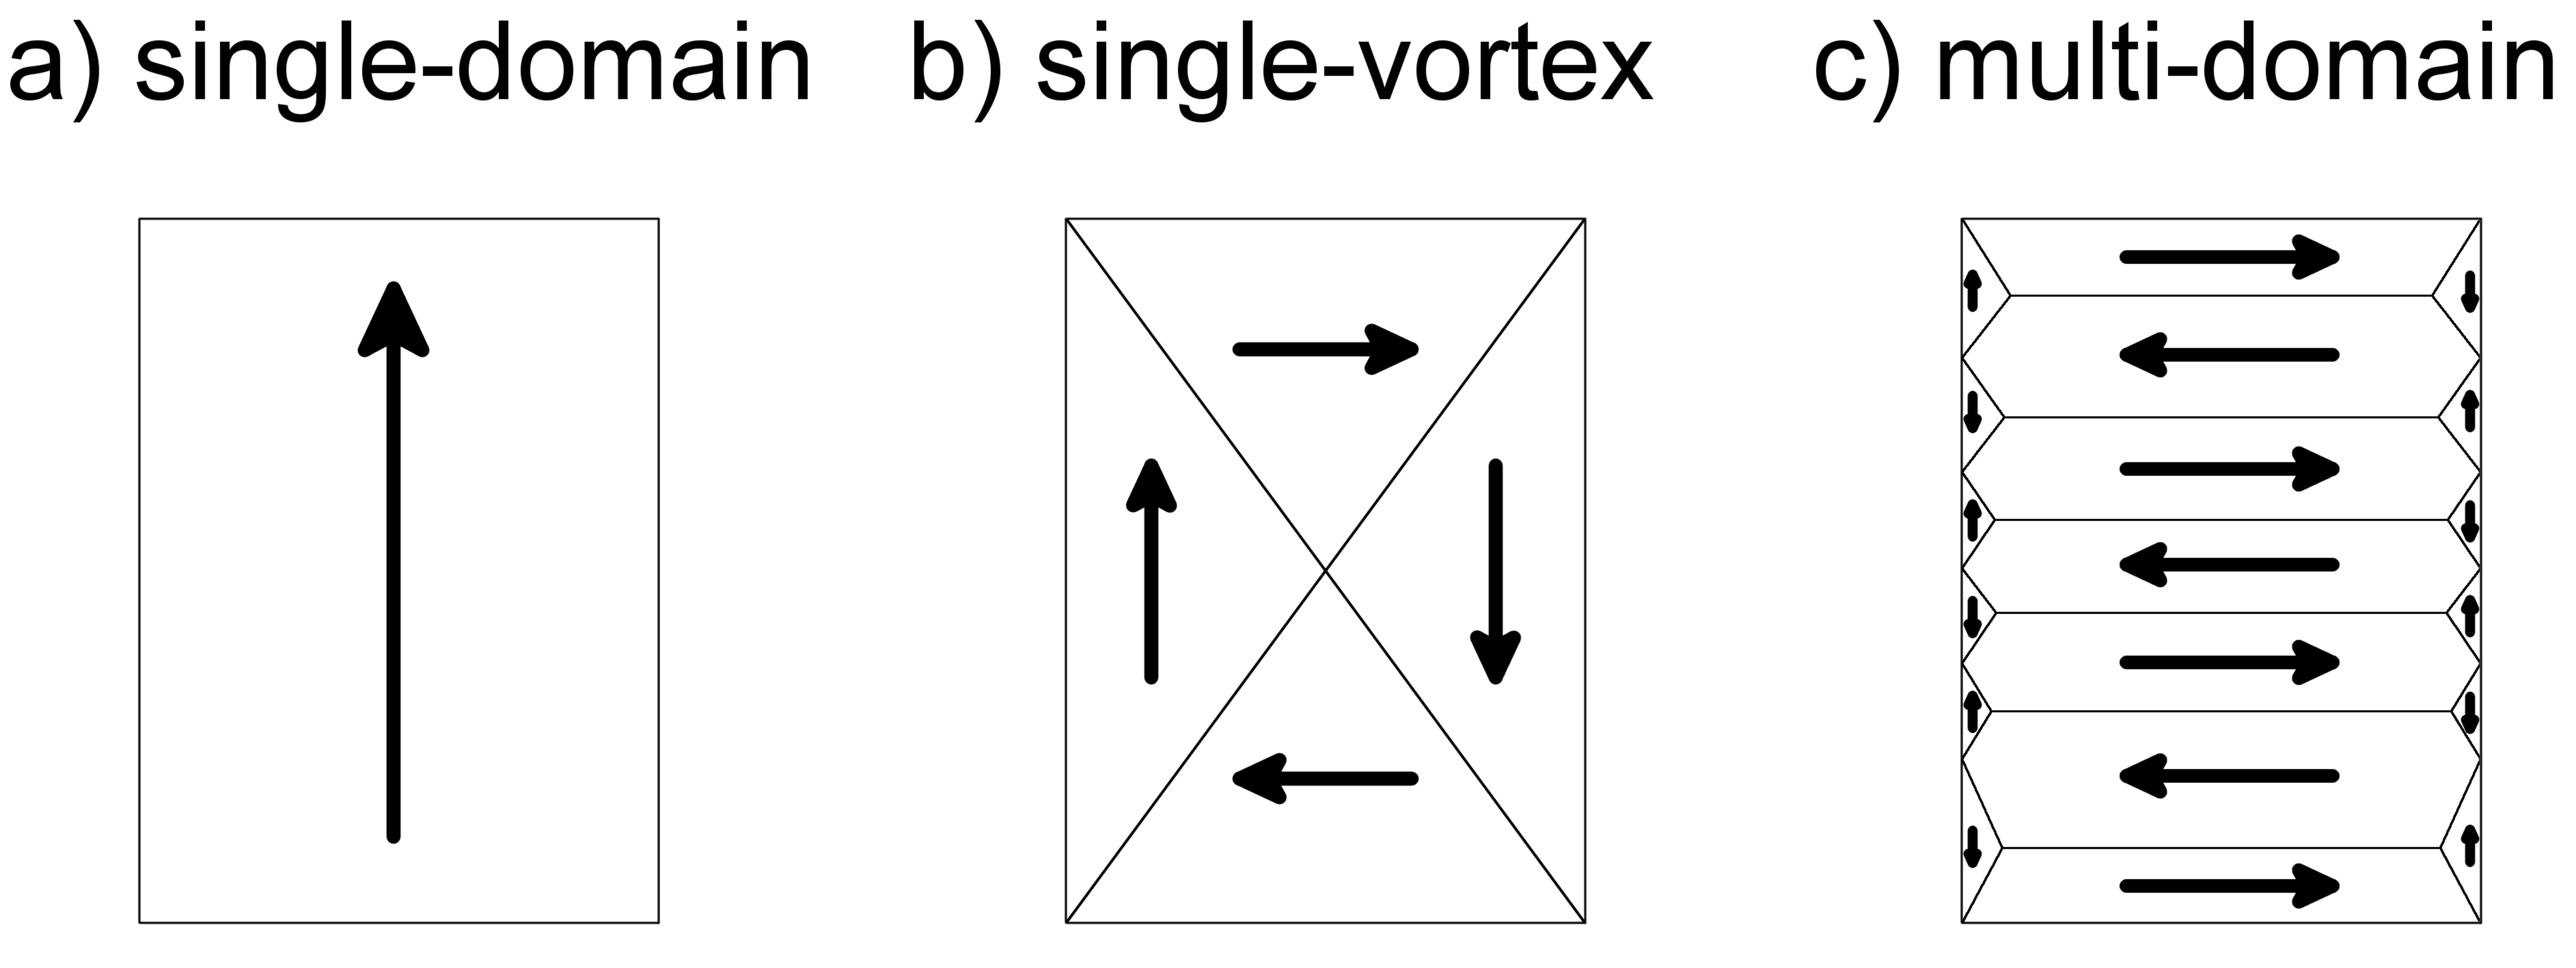
\includegraphics[width=\textwidth]{intro/figs/schematic_domains.pdf}
\caption[Domain state schematic]{Domain state schematic. Single-domain particles (a) are uniformly magnetised (highest magnetic moment). With increasing size, the magnetisation curls into a single-vortex state (b) (lower magnetic moment). In larger particles, the magnetisation is arranged in a multi-domain state (c) with regions called magnetic domains uniformly magnetised (lowest magnetic moment).}
\label{schematic_domains}
\end{figure}\par

Airborne magnetic surveys over oil fields \citep{Donovan1979} have revealed magnetic anomalies, i.e., measurable variations in the background magnetic field. \citet{Donovan1979} suggested that these anomalies are caused by the creation of authigenic near-surface magnetite in an environment of hydrocarbon seepage from the underlying reservoir. Further studies by \citet{Donovan1984}, \citet{Elmore1993} and \citet{Reynolds1993} in the U.S.A., \citet{Diaz2000}, \citet{Costanzo2006,Costanzo2012}, \citet{Gonzalez2002}, \citet{Guzman2011} in Venezuela and \citet{Liu1999}, \citet{Liu2004,Liu2006} in China have provided strong evidence for a genetic relationship between the magnetic contrasts produced by ferrimagnetic minerals near the surface and the underlying reservoir. These investigations confirm the original hypothesis \citep{Donovan1979} that the reducing environment caused by the upward seepage from the reservoirs is conducive to the formation of magnetic minerals such as magnetite and other iron oxides, greigite and other iron sulphides and depletion of minerals such as hematite \citep{Machel1991}, thus furthering the case for using a combination of aeromagnetic surveying and rock-magnetic measurements of soils and rocks for hydrocarbon prospecting.\par

Authigenic formation of magnetic minerals under hydrocarbon-producing conditions has been confirmed by \citet{Abubakar2015}; however, discussion on the exact mechanism for the formation of these minerals at different depths is ongoing. \citet{Machel1991} have identified two primary agents for the precipitation of magnetic minerals under the influence of hydrocarbon seepage. At higher temperatures and thus greater depths they propose chemical processes as the main factor while at shallower depths and lower temperatures it is argued that microbial sulphate-reducing processes are playing the larger role. \citet{Machel1991} also emphasised the difficulty in linking a magnetic anomaly to a process of hydrocarbon seepage because the precipitation of magnetic minerals can cause positive or negative anomalies---that is, peaks or dips in the geomagnetic field and the magnetic susceptibility of the soils. Nevertheless, careful analysis of the local conditions can result in the successful application of rock-magnetic measurements to hydrocarbon exploration \citep{Donovan1984,Liu2006,Emmerton2013B}. Magnetisation of oil-bearing rocks can also be used to assess the quality of oil \citep{Emmerton2013}. It was recognised by \citet{Reynolds1993} that in some cases iron sulphides are more important to the magnetic contrasts and thus to the identification of prospective oil-producing fields than iron oxides. Particularly, greigite (Fig. \ref{fram_oil}) has been identified as an authigenic mineral of the utmost importance \citep{Reynolds1993}.
\begin{figure}
\centering
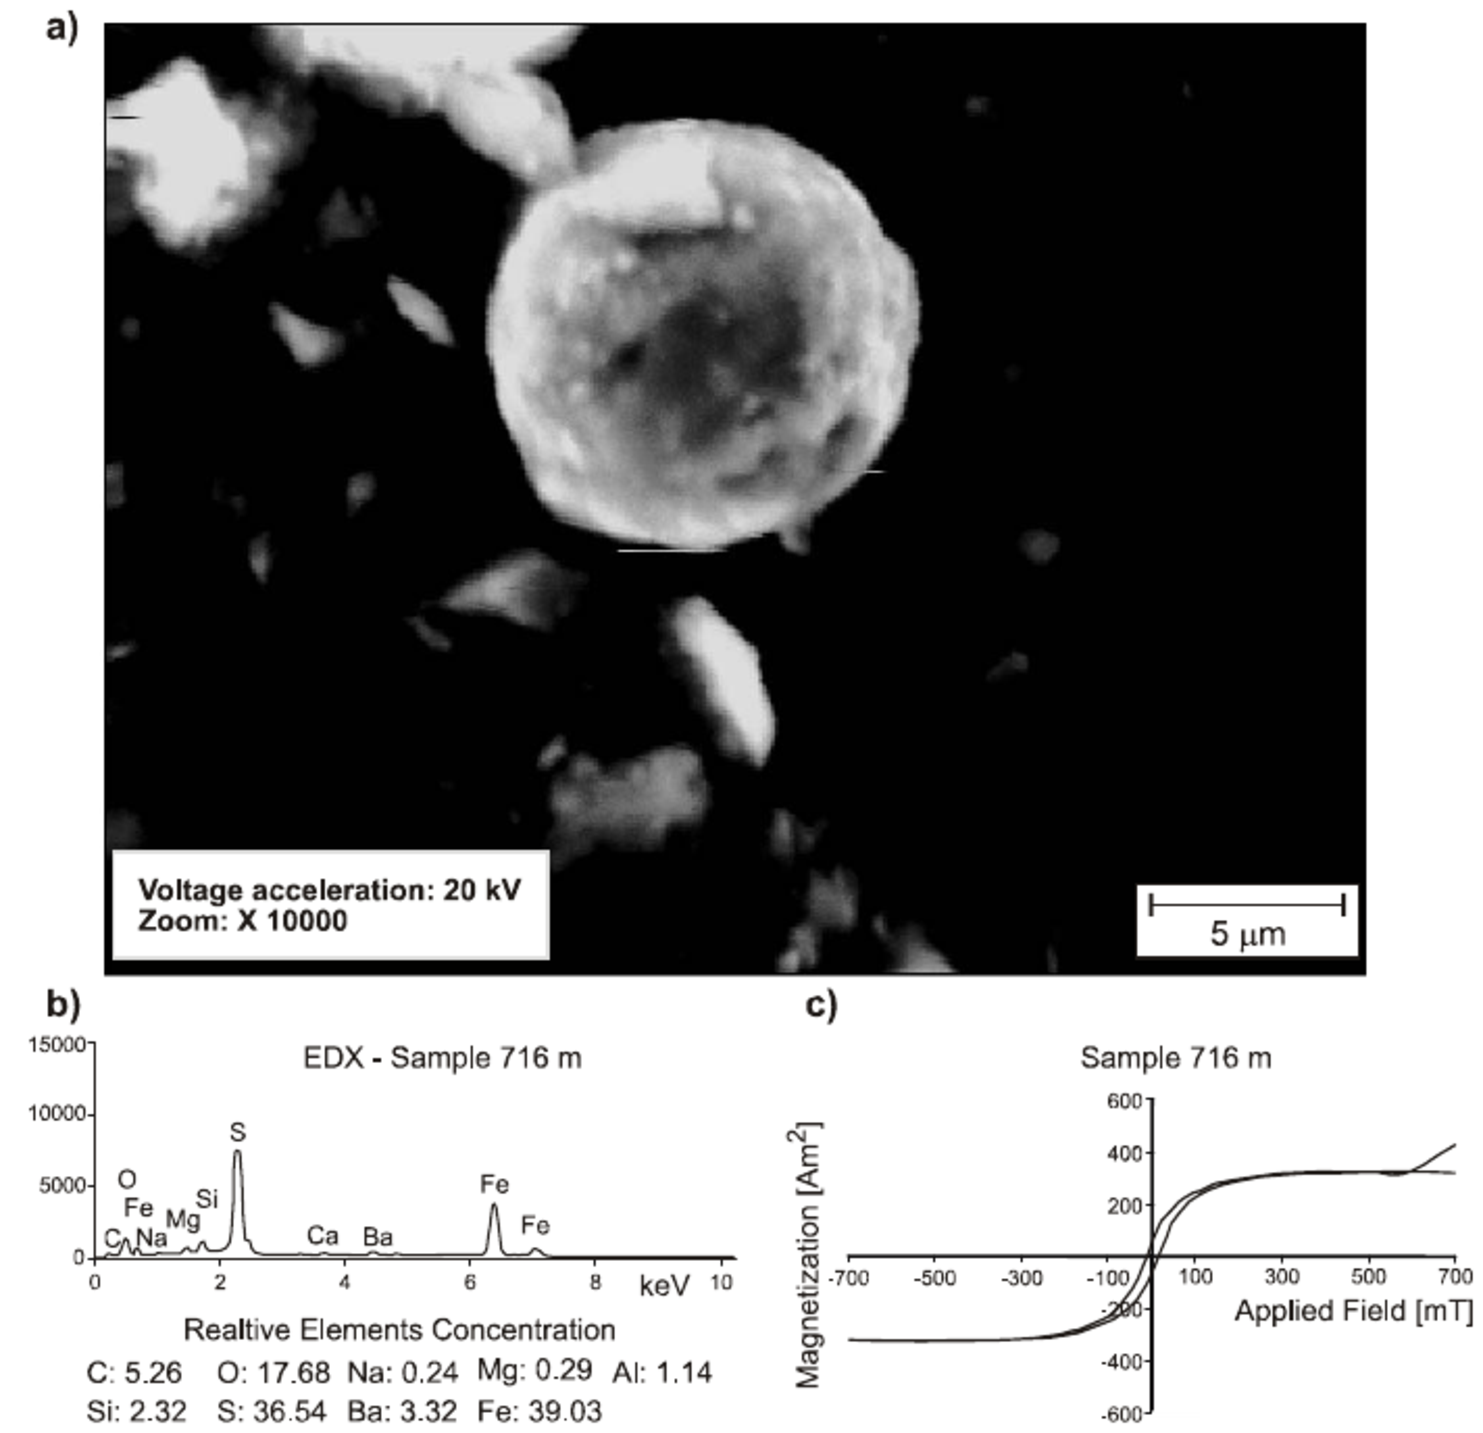
\includegraphics[width=\textwidth]{intro/figs/framboid_oil.pdf}
\caption[Greigite associated to hydrocarbon related magnetic contrasts]{Greigite associated to magnetic contrasts in hydrocarbon reservoirs. a) Scanning electron microscope micrograph and b) energy-dispersive X-ray spectroscopy analysis from the magnetic fraction of drill cuttings show spherical aggregates of minerals with high Fe and S content (likely greigite). c) Hysteresis curves for the same sample support the presence of ferrimagnetic minerals. (From \citet{Guzman2011}, reproduced with permission from the author).}
\label{fram_oil}
\end{figure}
\par

Greigite, first discovered in lacustrine sediments \citep{Skinner1964}, is an iron sulphide (Fe$_3$S$_4$) that can be thought of as the sulphide equivalent of the iron oxide magnetite (Fe$_3$O$_4$) as they have the same crystal structure only with sulphur replacing oxygen. Like magnetite, it is highly magnetic \citep{Li2014}. It is commonly formed authigenically in diagenetic anoxic sulphate-reducing sediments \citep{Roberts2011} as a precursor to pyrite \citep{Berner1984,Hunger2007}. Because of its unstable and precursory nature, its importance as a palaeomagnetic recorder has not been as readily realised as that of magnetite. However, geochemical conditions in sediments that are conducive to the long-term preservation of greigite are not uncommon \citep{Roberts2011,Roberts2015} and so, greigite is an important carrier of natural remanent magnetisation (NRM) in many systems \citep{Reynolds1994,Snowball1997,Ron2007,Roberts2010}.\par

Magnetic mineral grains that are linked to hydrocarbon seepage have sizes $\leq 30 \nm$ and thus generally in the SD range \citep{Liu2006}. In terms of morphology, it has been repeatedly found \citep{Ariztegui1996,Snowball1997,Aldana1999,Rowan2006,Roberts2010,Roberts2015} that equant grains of greigite assemble in raspberry-shaped aggregates (Fig. \ref{intro_01}) called framboids (from the French \textit{framboise} meaning raspberry). Presence of magnetic particle framboidal clusters has been linked to chemical alterations produced by hydrocarbon seepage \citep{Aldana1999} and to palaeoclimatic conditions \citep{Ariztegui1996}.\par

Given the unstable nature of greigite and the difficulties to produce synthetic samples, numerical investigations have the potential to answer important questions about greigite that can have great impact on magnetic hydrocarbon exploration and environmental magnetic studies. It is important that the fundamental magnetic parameters of greigite are precisely known to create accurate numerical models. Fabrication of higly pure synthetic greigite allowed \citet{Chang2008} to measure the saturation magnetisation $M_\text{S}$ and the exchange stiffness constant $A$; \citet{Li2014} improved the measurement of the saturation magnetisation. \citet{Winklhofer2014} measured the first estimates for the magnetocrystalline anisotropy (MCA) constants. These studies allow now for accurate models of greigite magnetisations.
\begin{figure}
\centering
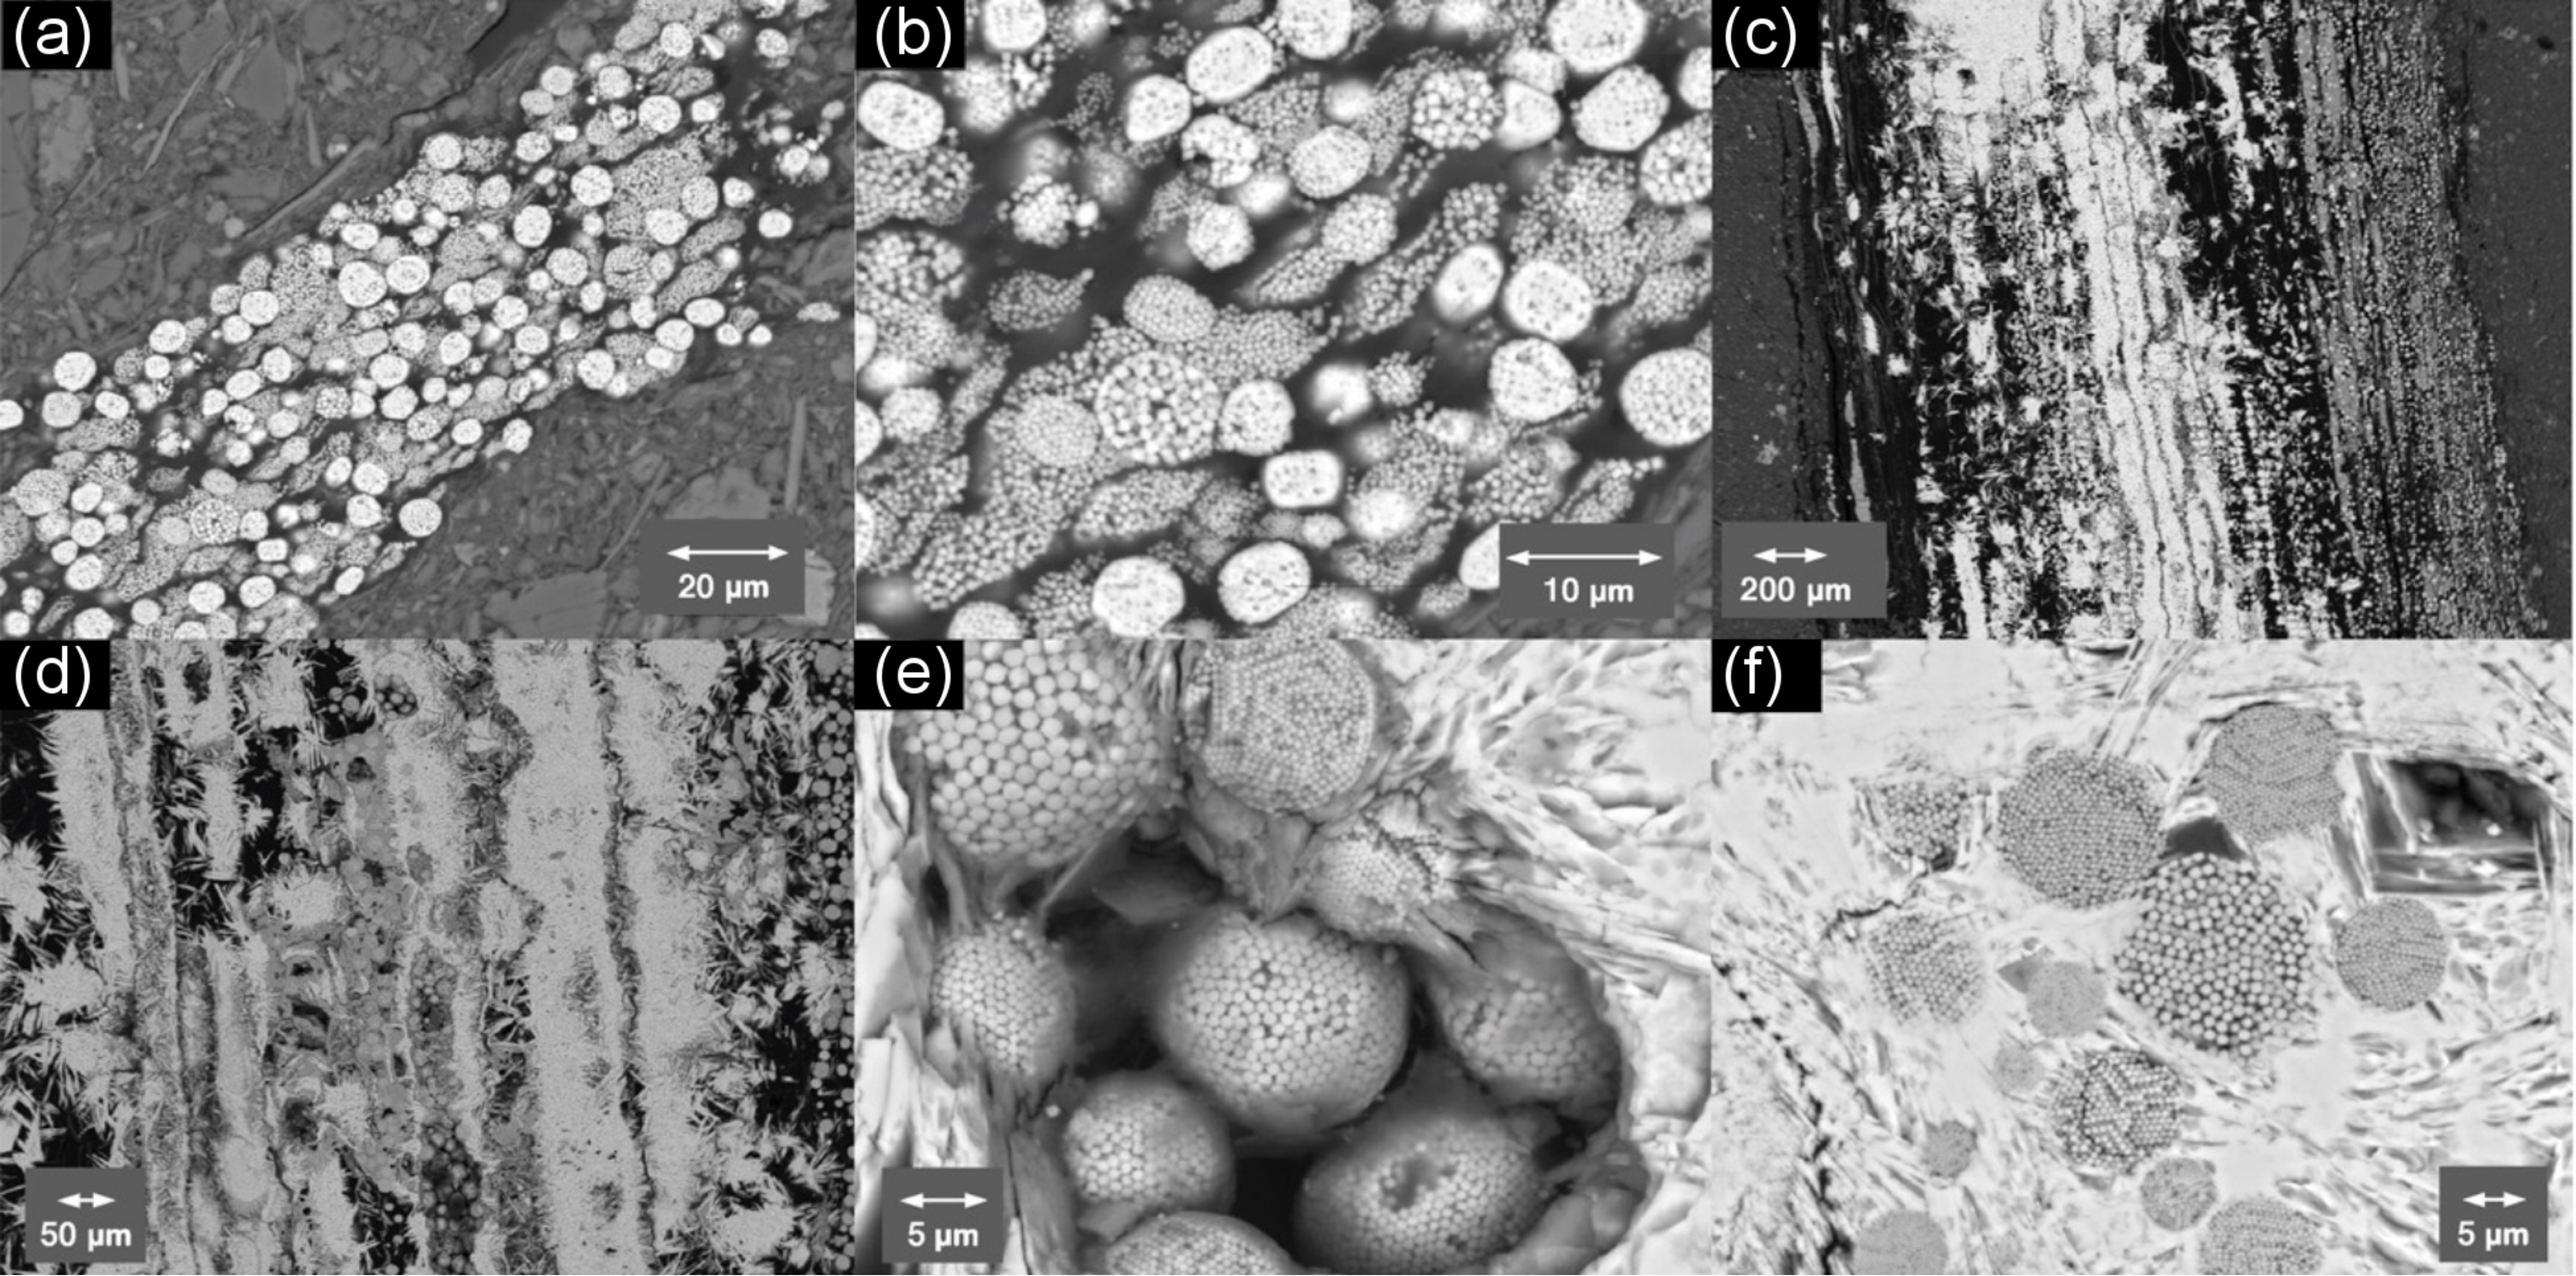
\includegraphics[width=\textwidth]{intro/figs/greigite_framboids_edit.pdf}
\caption[SEM images of framboidal greigite]{Scanning electron microscopy images of iron sulphide minerals. Elongated framboids and non-framboidal pyrite aggregates that probably represent remineralisation of plant cellular matter(a, b). Images at progressively higher magnification of an iron sulphide nodule with evidence of plant matter remineralisation (c--f). The platey minerals are non-magnetic hexagonal pyrrhotite. In (e), a void within the polished surface reveals a cluster of greigite (finest-grained) and pyrite (coarser-grained) framboids that have been overgrown by pyrrhotite (platey texture). (From \citet{Roberts2015}, reproduced with permission from the author).}
\label{intro_01}
\end{figure}
\par

In this thesis, numerical methods are employed to answer some fundamental questions about the magnetic properties of greigite:
\begin{itemize}
\item How does shape and size effect the magnetic structure in sub-micronic greigite?
\item What is the critical size at which greigite can no longer be SD?
\item Can greigite carry stable magnetisations over geological scales?
\end{itemize}
Also, it is important to answer some questions on how these properties effect bulk measurements commonly used for the identification of greigite. In this thesis, the focus is on hysteresis \citep{Mayergoyz1986} and first-order reversal curve (FORC) \citep{Roberts2000} properties:
\begin{itemize}
\item What is the hysteresis and FORC signal of non-interacting SD greigite ensembles?
\item What effect does SV magnetisations have on the non-interacting FORC response?
\item What is the FORC response of framboidal aggregates of greigite?
\end{itemize}
Answers to these questions have the potential to aid identification of greigite associated with magnetic constrasts over oil reservoirs.\par

\section{The iron sulphide greigite}
\subsection{Greigite occurrence in sediments}
In sulphide-rich sediments, ubiquitous redox reactions cause magnetic iron oxide minerals like magnetite and hematite to be replaced by iron sulphides \citep{Roberts2015}, most commonly pyrite \citep{Berner1984}. Pyrite is a paramagnetic mineral, and thus does not carry a permanent magnetisation. The replacement of magnetite and hematite for pyrite has important consequences for palaeomagnetic analyses of sediments as it can cause the effective destruction of the palaeomagnetic signal \citep{Rowan2009}. This process is pervasive in continental margin marine sediments with high organic carbon contents \citep{Roberts2015}. However, if the rate of Fe$^{2{+}}$ supply exceeds H$_2$S production (e.g. by sulphate-reducing bacteria), iron sulphides that form as precursors to pyrite formation (like greigite) can be preserved \citep{Berner1984}. Greigite can form early during sediment burial \citep{Reynolds1999} or at a later stage, remagnetising the host sediment \citep{Roberts2005} depending on the chronological sequence of the availability of the reactants conducive to greigite preservation. Identification of greigite and the timing of its formation is therefore critical for the magnetic interpretation of sediments.\par

\subsection{Greigite textures: framboidal clusters}
Iron sulphide textures can provide important environmental information about the early sedimentary conditions \citep{Roberts2015}. It is, then, important to identify the texture in which greigite occurs. Among the possible greigite textures, framboidal greigite has been identified as widespread \citep{Ariztegui1996,Wilkin1997} and potentially related to hydrocarbon migration \citep{Aldana1999}.\par

Framboids are spherical aggregates of greigite nano-crystals in which all the crystallites have the same size (Fig. \ref{intro_01}). Greigite and pyrite are often found in framboidal clusters and greigite also filling the space in a less organised manner \citep{Wilkin1997,Roberts2005,Roberts2010,Rowan2006}. Framboid origin is still debated, although some conclusions have been proposed. This morphology does not require biological activity \citep{Sweeney1973,Wilkin1996} although abundance of framboidal greigite is associated with high organic content. It is argued that formation of framboidal greigite is a necessary precursor to pyrite framboids \citep{Sweeney1973,Wilkin1997}. Greigite framboids have been widely observed and the constituent nanocrystals are always finer-grained than neighbouring pyrite crystals \citep{Ariztegui1996,Roberts2005,Roberts2010,Rowan2006}. This is consistent with the pyrite framboid formation process proposed by \citet{Wilkin1997}:
\begin{enumerate}
\item nucleation of iron monosulphide (FeS, mackinawite) nanocrystals,
\item chemical alteration of these into greigite (Fe$_3$S$_4$),
\item aggregation of greigite nanocrystals with uniform sizes to form framboids,
\item replacement of greigite by pyrite (FeS$_2$).
\end{enumerate}
Alternatively, the geochemical balance between iron and sulphur can impede the replacement of greigite by pyrite, leading to greigite preservation.\par

Independently of formation mechanism, an important aspect of greigite and pyrite framboids is that the nanocrystals in all framboids have uniform particle sizes \citep{Wilkin1996}. This is a potential indication that the crystallites nucleated simultaneously, at the same growth rate and thus all under the same geochemical conditions. This is an important observation with potential applications for the timing of sulphidisation events on a geological timescale. Because of this, identification of framboidal greigite is an important problem for environmental magnetic studies. Occurences of magnetite framboids in meteoritic samples have also been observed \citep{Astafieva2004,Kimura2013}; therefore, magnetic mineral framboidal textures are widespread and identification via rock magnetic measurements is an important problem.\par

\subsection{Fundamental magnetic parameters of greigite}
The fundamental magnetic parameters of greigite used throughout this investigation are the saturation magnetisation $M_\text{S}=3.51\,\mu_\text{B}\,\text{p.c.u.}$ \citep{Li2014} or $\roughly 2.7 \times 10^5\,\text{A/m}$  which is $\roughly$11\% higher than the value previously reported by \citet{Chang2009} of $3.25\,\mu_\text{B}$ p.c.u. (and $\roughly$57\% the value of  $M_\text{S}$ for magnetite). \citet{Li2014} synthesised highly pure, high-crystallinity greigite samples on which $M(H)$ hysteresis curves were measured. The saturation magnetisation was estimated from a nonlinear fitting $M(H)=M_{\text{S}}(1-aH^{-1} + b{H^{-2}}) + cH^{1/2}$ where $a,\, b,\, c$ are constants that describe the structural inhomogeneity within the sample, the magnetic anisotropy energy, and the paramagnetic effect caused by the applied field, respectively. Microstructural inhomogeneities determine the low field response whereas the approach to saturation is determined by the anisotropy \citep{Li2014}. The obtained room-temperature value of $M_\text{S}=3.51\,\mu_\text{B}\,\text{p.c.u.}$ is lower than the value of $4\,\mu_\text{B}\,\text{p.c.u.}$ predicted from a purely ionic model \citep{Coey1970}, this is due to the degree of covalency of the Fe--S bond as well as the possible canting of surface spins induced by surfactant molecules bonded to the surface \citep{Li2014}. Of the magnetic parameters used for the purposes of this work, the value of the saturation magnetisation is the most accurate.\par

\citet{Winklhofer2014} used ferromagnetic resonance spectroscopy to estimate the anisotropy constants. They obtained a (first) cubic MCA constant $K_1=-1.7\times10^4\,\text{J}/\text{m}^3$ and negligible second MCA constant $K_2$ to $K_1$ ratio, i.e., the easy axes are the $<$111$>$. The data was consistent, as well, with a positive value for $K_1$ and large $K_2\approx 3K_1$ and thus $<$100$>$ easy axes; however, there is indirect \citep{Winklhofer2014} and direct \citep{Li2014} evidence favouring the anisotropy model with negative $K_1$ which we use throughout this work.\par

The exchange stiffness constant was estimated by \citet{Chang2008} to be $A=2\times10^{-12}\,\text{J}/\text{m}$. The exchange energy in a ferrimagnet is related to the spin wave stiffness. Experimental observation of spin waves can be achieved by several methods, e.g., inelastic neutron scattering and spin wave resonance. These experimental techniques require, however, relatively large, uniform crystals on which to observe spin wave propagation. Since fabrication of such samples is as yet impossible for greigite, \citet{Chang2008} measured the saturation magnetisation (in a field of $5\,\text{T}$) of powdered greigite samples at low temperatures. Using the spin wave expansion of the spontaneous magnetisation for low temperatures $M(T)=M_{\text{S}}(1-CT^{3/2})$ \citep{Bloch1932}, where $C$ is a function of the spin wave stiffness, they were able to fit the data and obtain an estimate of the spin wave stiffness and therefore the exchange stiffness constant. Determination of the spin wave stiffness through different approaches like inelastic neutron scattering \citep{Torrie1967}, low-temperature heat capacity \citep{Kenan1963} and low-temperature $M_{\text{S}}$ measurements \citep{Aragon1992}, however, has been known to produce variable results for magnetite \citep{Chang2008}. This places a degree of uncertainty on this measurement for greigite that is hard to quantify in the absence of measurements acquired through means other than low-temperature saturation magnetisation.\par

Chemical alteration of greigite at high temperatures has made difficult to measure accurately the Curie temperature; however, there is strong evidence for a Curie temperature $T_\text{C}>620\,\text{K}$ \citep{Roberts2010}. The exchange energy is directly related to $T_\text{C}$; within a mean field approximation \citep{Kouvel1956}:
\begin{equation}
T_\text{C} = \frac{4\sqrt{2} J_\text{AB}}{K_\text{B}}\sqrt{S_\text{A}S_\text{B}(S_\text{A}+1)(S_\text{B}+1)},
\end{equation}
where $K_\text{B}$ is Boltzmann's constant, $J_\text{AB}$ is the exchange integral between A- and B-sites and $S_\text{A},\, S_\text{B}$ the spin magnetic moments of sites A and B, respectively. Plugging in the relatively low value of $J_\text{AB}\approx 1\,\text{meV}$ measured by \citet{Chang2008} and $S_\text{A}=1.54$, $S_\text{A}=1.63$ \citep{Chang2009} predicts a low $T_\text{C} \approx 260-287 \, \text{K}$. This suggests the uncertainty in the measurement of $A$ by \citet{Chang2008} is significant. A value of $J_\text{AB}=2.31\,\text{meV}$ results in a $T_\text{C}\approx 620\,\text{K}$. However, mean field approximations tend to overestimate the Curie temperature, so the value of the exchange integral $J_\text{AB}$ could be up to 4 times the value reported by \citet{Chang2008}. Throughout this work the value of \citet{Chang2008} is used. Increased values of $A$ have the effect of increasing the domain wall width and thus the critical size $d_0$; a calculation of the SD to SV critical size $d_0$ was done for values $A=4\times10^{-12}\,\text{J}/\text{m}$ and $A=8\times10^{-12}\,\text{J}/\text{m}$ (Chapter \ref{ch:res-1}) to quantify this effect. Changes in the exchange stiffness constant have little effects on the coercivities of SD and possibly SV grains. Uncertainty in this parameter can modify the absolute values of some of the magnetic properties simulated in this work, however, the physics should remain mostly unaffected.\par

\section{Magnetism and matter}
For the purposes of the thesis, a brief review of fundamental concepts of magnetism follows.\par
 
\subsection{Fundamentals of magnetism}
The magnetic induction field $\boldsymbol{B}$, like the electric field $\boldsymbol{E}$, is defined by its effect on a \textit{test particle}, namely, the Lorentz force \citep{Feynman}:
\begin{equation}\label{lorentz}
\boldsymbol{F}_\text{Lorentz} = q(\boldsymbol{E} + \boldsymbol{v}\times\boldsymbol{B}),
\end{equation}
where $q$ is the electrical charge of the test particle and $\boldsymbol{v}$ its velocity. The force a magnetic $\boldsymbol{B}$ field exerts on a moving electrical charge is perpendicular to both its velocity and to the field itself. From Eq. \ref{lorentz}, the units of $\boldsymbol{B}$ are $\text{N}/(\text{C}\cdot\frac{\text{m}}{\text{s}})$, this physically meaningful unit (one Newton of force per charge of one Coulomb moving at one meter per second) is called Tesla, with symbol $\text{T}$.\par

When describing magnetic fields, a distinction between the magnetic induction $\boldsymbol{B}$ and the magnetic field $\boldsymbol{H}$ is made. These denominations, however, are of historical character; it can be proved that the fundamental field is the induction field $\boldsymbol{B}$ \citep{Feynman}. In a vacuum, $\boldsymbol{B}$ and $\boldsymbol{H}$ coincide in direction. In the SI the magnetic and induction fields differ by a scalar factor $\mu_0$, the \textit{magnetic constant}, also known as the vacuum permeability or permeability of free space:
\begin{equation}
\mu_0 = \frac{B_{\text{vacuum}}}{H_{\text{vacuum}}} = 4 \pi \times 10^{-7} \, \text{T}\cdot\frac{\text{m}}{\text{A}}.
\end{equation}
Although the names vacuum permeability and permeability of free space are still widespread it is preferable to use the name magnetic constant since it reflects the fact that it is a defined value and not a measurement.\par

The description of magnetic fields is analogue to that of electrical fields. Although, unlike the situation in electricity, there are no magnetic charges, only magnetic dipoles \citep{Feynman}. The induction due to a wire carrying a current $I$ (generally varying along the path) at a point $\boldsymbol{r}$ can be calculated from the Biot-Savart law:
\begin{equation}
\boldsymbol{B}(\boldsymbol{r}) = \frac{\mu_0}{4\pi} \int_C \frac{I\, \text{d}\boldsymbol{l}\, \times \, \boldsymbol{r}}{r^3},
\end{equation}
where $\text{d}\boldsymbol{l}$ is a differential element of length along the wire in the direction of the current. The integral is carried out along a line, usually but not necessarily a closed curve.\par

In general, it is more interesting and important to consider magnetism in the presence of matter. A material is composed of atoms, which individually may hold a permanent magnetic dipole moment $\boldsymbol{\mu}$ (with units $\text{A}\cdot \text{m}^2$). The \textit{magnetisation} vector field $\boldsymbol{M}$ (with constant norm $|\boldsymbol{M}|=M_\text{S}$) is the spatial average of a myriad of these individual atomic dipole moments over a suitable volume. Therefore, $\boldsymbol{M}$ accounts for the contribution of atomic magnetic moments to the total field. In the SI units we have
\begin{equation}
\boldsymbol{B} = \mu_0 (\boldsymbol{H}+\boldsymbol{M});
\end{equation}
$\boldsymbol{H}$ and $\boldsymbol{M}$ have the same units, the Ampere per meter $\text{A}/\text{m}$. The meaning of this unit is somewhat obscured, but made evident if written in the form $\text{A}/\text{m} = \text{A}\cdot\text{m}^2/\text{m}^3$, i.e., this unit can be thought of as a density of magnetic moments.\par

\subsection{Diamagnetism and paramagnetism}
Magnetism in matter can be broadly categorised into three phenomena: diamagnetism, paramagnetism and ferromagnetism. Diamagnetism and paramagnetism are of little importance to this work so will be only briefly described.\par

Diamagnetism is a property of all matter. It is the smallest effect and is a tendency of a material to oppose an external magnetic field. An external magnetic field exerts a Lorentz force on the bound electrons that causes them to precess like a gyroscope. This is called Larmor precession and is equivalent to an electric current producing a magnetic moment in the direction opposed to the external $\boldsymbol{B}$ field. Water is a common example of a highly diamagnetic material.\par

Paramagnetism is a partial alignment of the atomic magnetic moments of the atoms in a material with an external $\boldsymbol{B}$ field. It is only thermal noise that prevents a perfect alignment of the atomic magnetic moments with the external field, therefore this is a highly temperature dependent phenomenon. Nevertheless, at ordinary temperatures, paramagnetism outweighs diamagnetism by a factor greater than 10.\par

In both diamagnetism and paramagnetism a magnetisation is induced by an external field. The rate at which the magnetisation is acquired with respect to the applied field is called the \textit{magnetic susceptibility} $\chi = \frac{\text{d}\boldsymbol{M}}{\text{d}\boldsymbol{H}}$, in general a tensor.\par

\subsection{Ferromagnetism}
A ferromagnetic material, in contrast with diamagnetic and paramagnetic materials, can retain a (non-saturated) remanent magnetisation in the absence of an external field. In the presence of a relatively weak external field, ferromagnetic materials acquire magnetisations thousands of times stronger than paramagnetic materials. To reconcile these two observations, \cite{Weiss1906} proposed that in ferromagnetic materials there exist magnetic domains, regions which are locally magnetised to saturation, brought about by an \emph{ad-hoc} molecular field; when there is an external field, domains aligned with the field would grow and/or the domains would rotate with the field and when the field is removed the domains would return to random alignments thereby reducing the net magnetisation of the body. Although domain theory was succesful in explaining important aspects of ferromagnetic behaviour, the theory was unsatisfying as it did not explain the origin of the molecular field \citep{Kittel1949}.

Ultimately, ferromagnetism is a phenomenon that cannot be explained solely by classical physics. At the core is the quantum-mechanical concept of exchange coupling, a phenomenon with no classical counterpart \citep{Heisenberg1926}. The origin of ferromagnetism is the alignment of atomic moments (electron spins) by quantum exchange forces. However, in a narrower sense, ferromagnetic materials are those in which \emph{all} the atomic moments share the same alignment. There is a class of materials in which the quantum exchange forces create anti-parallel alignments between atomic moments in different sublattices. When the net magnetic moment of one sublattice is smaller than that of the other, there remains a net moment: these are the ferrimagnetic materials. When the magnetic moments of the different sublattices cancel there is no net magnetic moment: these are the antiferromagnetic materials. Throughout the thesis, the term ferromagnetism is used in a broad sense to include ferrimagnetic behaviour.\par

Exchange coupling is hindered by thermal noise, i.e., ferromagnetic behaviour weakens with increasing temperature. There is a threshold temperature beyond which thermal fluctuations destroy all magnetic ordering and the material becomes paramagnetic; this is the Curie temperature $T_\text{C}$, characteristic of a ferromagnetic material.\par

\citet{Landau1935} obtained a continuum expression for the exchange energy. The main result in \citet{Landau1935} was the theoretical proof that inside a ferromagnetic material there are regions that are magnetised to saturation: the magnetic domains, and that between these domains exist regions where the magnetisation continuously rotates from the direction of one domain to that of the other; these are called \textit{domain walls}. The calculation of \citet{Landau1935} of magnetic domain size and domain wall width and speed of propagation was the first micromagnetic calculation \citep{Brown}.

\section{Micromagnetics}\label{mmsection}
\citet{Brown} recognised that there was a need for a robust theory on a scale large enough to treat ferromagnetic bodies as a a continuum and small enough to capture the magnetic structure at sub-micron lengths. He called such a theory micromagnetics. The seminal work of \citet{Landau1935} and that of \citet{Brown} are the theoretical basis from which micromagnetics emerged. Micromagnetics is the theory that bridges the fundamental quantum-mechanical picture and the effective macroscopic theory of Maxwell equations. The main goal of micromagnetics is to obtain a configuration of the magnetisation vector $\boldsymbol{M}$ in a ferromagnetic material.\par

\subsection{Magnetic Gibbs free energy}
There are two main approaches to micromagnetism. One is to obtain a configuration of the magnetisation in a ferromagnetic material by minimising the magnetic Gibbs free energy. The other is to solve a partial differential equation (PDE) that describes the dynamics of the magnetic moments; this equation was derived by \citet{Landau1935} and improved by \citet{Gilbert2004} to include damping effects, the Landau-Lifshitz-Gilbert (LLG) equation.\par

It is known from thermodynamics that starting from a nonequilibrium state the evolution of a system can only be such that its Gibbs free energy diminishes. So, by an explicit formulation of the different energies contributing to the total magnetic Gibbs free energy it is possible to find a configuration that is either a local energy minimum (LEM) or global energy minimum (GEM). One of the biggest contributions of micromagnetics to our understanding of magnetic phenomena in matter is that it is quite common for a material to be in a LEM configuration rather than GEM. This is the cause of magnetic hysteresis and magnetic remanence. Disregarding thermal effects and magnetostrictive forces, four magnetic energies contribute to the total. There are microscopic contributions like the exchange energy and the MCA energy. Also macroscopic contributions like the magnetostatic self-energy and the external field energy. The external field is independent of the magnetisation and the exchange and anisotropy energies are short range so these are very easy to calculate. The magnetostatic self-energy, i.e., the interaction between the magnetic moments in the material and the stray field the magnetic body produces is a long range, non-local interaction. This energy creates a demagnetising effect.\par

We can write the total magnetic Gibbs free energy $E_\text{G}$ as the integral of the sum of energy densities $\phi$ associated with these effects \citep{Brown}:
\begin{equation}\label{gibbs0}
E_{\text{G}} = \int_{\Omega} (\phi_{\text{exchange}} + \phi_{\text{anisotropy}} + \phi_{\text{stray}} + \phi_{\text{external}})\, \text{d}^3\boldsymbol{r},
\end{equation}
where $\Omega$ is the ferromagnetic volume and $\text{d}^3\boldsymbol{r}$ the volume differential.\par

The exchange energy is a quantum-mechanical phenomenon wherein the exchange of inner shell electrons between neighbouring atoms results in spin-exchange coupling. The continuum expression was obtained by \citet{Landau1935} and found to be proportional, up to a constant, to the square of the gradient of the magnetisation distribution:
\begin{equation}
\phi_{\text{exchange}} = A | \nabla \boldsymbol{m} |^2,
\end{equation}
where $A$ is the exchange stiffness constant and $\boldsymbol{m}$ is the reduced magnetisation vector, i.e., $\boldsymbol{m}$ is a unit vector in the direction of the magnetisation. This energy density is minimised for uniform magnetisations, therefore, the effect of the exchange energy is to homogenise the distribution of moments.\par

MCA energy is due to the atomic configuration of a crystalline material. The specific arrangement of atoms in the crystal can cause some directions to be easier for the moments to align with \citep{Kittel1949}. These directions are called easy axes. The anisotropy energy of a cubic crystal is given by:
\begin{equation}
\phi_{\text{anisotropy}}=\frac{K_1}{2}\sum_{i\neq j}\gamma_i^2\gamma_j^2 + K_2\prod_i\gamma_i^2,
\end{equation}
where $\gamma_i$ are the magnetisation direction cosines and $K_1$, $K_2$ the first and second anisotropy constants. In terms of the reduced magnetisation vector components, this can be written as:
\begin{equation}
\phi_{\text{anisotropy}}=K_1(m_x^2m_y^2+m_y^2m_z^2+m_z^2m_x^2) + K_2m_x^2m_y^2m_z^2.
\end{equation}
The effect of the MCA energy is a tendency for the magnetic moments to align with the easy axes of magnetisation.\par

The external field energy is the potential energy associated with the interaction of the magnetic moments with an external field:
\begin{equation}
\phi_{\text{external}} = -\boldsymbol{M} \cdot \boldsymbol{B}_{\text{external}},
\end{equation}
where $\boldsymbol{B}_{\text{external}}$ is an external magnetic induction field. This energy tends to align the magnetic moments with the external field.\par

The magnetostatic self-energy is due to the magnetostatic interaction each magnetic moment has with each other. Because in a numerical micromagnetic model there can be hundreds of thousands of individual magnetic moments (mesh/grid points), this is energy is the most numerically expensive to calculate; many methods have been devised to avoid calculating this interaction for each moment, most of these based on the magnetic scalar potential.\par

A partial differential equation for the magnetic potential $\varphi$ is formulated of the form:
\begin{equation}\label{potential}
\nabla^2 \varphi(\boldsymbol{r}) =
\begin{cases}
4\pi\nabla \cdot \boldsymbol{M}, & \text{for }\boldsymbol{r} \in \Omega \\
0,                           & \text{for }\boldsymbol{r} \in \mathbb{R}^3 / \boldsymbol{\Omega};
\end{cases}
\end{equation}
with boundary conditions on the surface $\partial \Omega$:
\begin{align}\label{boundaries1}
\left. \left[ \varphi \right]\right|_{\partial \Omega} &= 0, \\
\left. \left[ \frac{\partial \varphi}{\partial \boldsymbol{\hat{n}}} \right]\right|_{\partial \Omega} &= -4\pi \boldsymbol{M} \cdot \boldsymbol{\hat{n}}, \label{boundaries2}
\end{align}
where $\left. \left[\cdots \right]\right|_{\partial \Omega}$ denotes a discontinuity across the boundary (surface) and $\boldsymbol{\hat{n}}$ an outward-pointing surface-normal unit vector. Also, a condition:
\begin{equation}\label{boundary}
\lim_{|\boldsymbol{r}| \to \infty} \varphi(\boldsymbol{r}) = 0
\end{equation}
must be met. Solving this sytem for $\varphi$ is sufficient to calculate the stray field from:
\begin{equation}
\boldsymbol{B}_\text{stray} = -\mu_0 \nabla \varphi.
\end{equation}\par

One of the principal difficulties in solving Eq. \ref{potential} is the limit condition (Eq. \ref{boundary}) because in numerical calculations it is impossible to formally evaluate the potential at infinity. \citet{Imhoff1990} proposed a transformation method that requires space surrounding the ferromagnetic body to be meshed into two concentric shells. The potential is mapped on the outer shell to infinity to satisfy the boundary conditions. A hybrid finite-element method (FEM) and boundary-element method (BEM) formulation \citep{Fredkin1990} does not require free space to be meshed, at the cost of the mathematical complexity involved in the hybrid scheme. In this scheme, the scalar magnetic potential is split $\varphi = \varphi_1 + \varphi_2$, where for $\boldsymbol{r} \in \Omega$, $\varphi_1$ is the solution to the inhomogenous Neumann problem:
\begin{equation}
\nabla^2 \varphi_1 = 4 \pi \nabla \cdot \boldsymbol{M}
\end{equation}
with the boundary condition
\begin{equation}
\left. \frac{\partial \varphi_1}{\partial \boldsymbol{\hat{n}}} \right|_{\partial \Omega} = 4 \pi \boldsymbol{M} \cdot \boldsymbol{\hat{n}},
\end{equation}
and $\varphi_1$ is defined $\varphi_1 = 0$ for $\boldsymbol{r} \in \mathbb{R}^3 / \Omega$. With this, $\varphi_2$ satisfies:
\begin{equation}
\nabla^2 \varphi_2 = 0,
\end{equation}
and from the boundary conditions (Eqs. \ref{boundaries1}, \ref{boundaries2}), there are conditions at the boundary:
\begin{align}
\left. \left[  \varphi_2 \right] \right|_{\partial\Omega} &= \varphi_1, \\
\left. \left[  \frac{\partial\varphi_2}{\partial\boldsymbol{\hat{n}}} \right] \right|_{\partial\Omega} &= 0;
\end{align}
a condition $\lim_{|\boldsymbol{r}| \to \infty} \varphi_2 = 0$ is also required. In practice, $\varphi_1$ is determined with a FEM which gives the boundary conditions to determine $\varphi_2$ via BEM.\par

The magnetostatic self-energy creates a demagnetising effect, that is, the field $\boldsymbol{B}_{\text{stray}}$ produced by the magnetisation distribution opposes the magnetisation. It is also the phenomenon that has the principal role in the domain structure of large particles. When this demagnetising field is calculated, the magnetostatic self-energy can be expressed as \citep{Brown}:
\begin{equation}
\phi_{\text{stray}} = -\frac{1}{2}\boldsymbol{M}\cdot\boldsymbol{B}_{\text{stray}},
\end{equation}\par
where the factor $1/2$ accounts for the interaction between all magnetic dipoles being counted twice when calculating $\boldsymbol{B}_\text{stray}$.\par

With these expressions for the energy densities, Eq. \ref{gibbs0} can now be rewritten as:
\begin{multline}
E_{\text{G}} = \int_{\Omega} \left( A| \nabla \boldsymbol{m} |^2  + K_1(m_x^2m_y^2+m_y^2m_z^2+m_z^2m_x^2) + K_2m_x^2m_y^2m_z^2 \right. \\
\left. - \boldsymbol{M} \cdot \boldsymbol{B}_{\text{external}} - -\frac{1}{2}\boldsymbol{M}\cdot\boldsymbol{B}_{\text{stray}} \right) \, \text{d}^3\boldsymbol{r}.
\end{multline}
A system out of equilibrium is spontaneously driven to diminish its free energy. The aim of a micromagnetic algorithm is to obtain a distribution of the magnetisation in equilibrum. \citet{Fischbacher2017} describes energy minimisation algorithms for the micromagnetic energy functional. \citet{Brown} proposed a variational method based on the variational derivative of the total energy with respect to the magnetisation. In equilibrium, the variation of the free energy vanishes
\begin{equation}
\frac{\delta E_{\text{G}}}{\delta\boldsymbol{m}} = 0.
\end{equation}
This leads to Brown's equation:
\begin{equation}
\boldsymbol{m} \times \left( \frac{2A}{M_\text{S}}\nabla^2\boldsymbol{m} + \boldsymbol{B}_\text{anisotropy} + \boldsymbol{B}_{\text{external}} + \boldsymbol{B}_{\text{stray}} \right) = 0,
\end{equation}
with $\boldsymbol{B}_\text{anisotropy} = \frac{1}{M_\text{S}}(2K_1m_x(1-m_x^2)+2K_2m_y^2m_z^2m_x)\ihat+(2K_1m_y(1-m_y^2)+2K_2m_z^2m_x^2m_y)\jhat+(2K_1m_z(1-m_z^2)+2K_2m_x^2m_y^2m_z)\boldsymbol{\hat{k}}$. This means that in equilibrium the magnetisation is parallel to an effective field:
\begin{equation}
\boldsymbol{B}_{\text{eff}} = \frac{2A}{M_s}\nabla^2\boldsymbol{m} + \boldsymbol{B}_\text{anisotropy} + \boldsymbol{B}_{\text{external}} + \boldsymbol{B}_{\text{stray}}=\mu_0 \boldsymbol{H}_\text{eff},
\end{equation}
and so, the torque (analogue) acting on the magnetic moments vanishes $\boldsymbol{m} \times \boldsymbol{B}_{\text{eff}} = 0$. This is the motivation to use a dynamical equation involving the torques produced by the effective field as an alternative to energy minimisation.\par

\subsection{The Landau-Lifshitz-Gilbert equation}
Finding an equilibrium magnetisation via energy minimisation (Eq. \ref{gibbs0}) may not always result in physically meaningful distributions. This is because in micromagnetic systems, the energy landscape is usually very complicated and contains many local maxima, minima and saddle points. A more physical approach is finding a solution to the dynamical problem. However, this is numerically more expensive than energy minimisation. The motion of a magnetic moment is mainly due to the Larmor precession around its local field. The Gilbert equation \citep{Gilbert2004} describes this precession and considers damping effects with a single damping constant:
\begin{equation}
\frac{\partial \boldsymbol{M}}{\partial t} = -\gamma\boldsymbol{M}\times\boldsymbol{H}_\text{eff} + \alpha\boldsymbol{M}\times\frac{\partial\boldsymbol{M}}{\partial t},
\end{equation}
where $\gamma = 2.210173 \times 10^5 \frac{\text{m}}{\text{A}\cdot\text{s}}$ is the gyromagnetic ratio and $\alpha$ a phenomenological damping parameter, characteristic of the material \citep{Gilbert2004}. An equivalent formulation is the LLG equation:
\begin{equation}
\frac{\partial\boldsymbol{M}}{\partial t} = -\gamma^{'} \boldsymbol{M}\times\boldsymbol{H}_\text{eff} - \frac{\alpha\gamma^{'}}{M_\text{S}} \boldsymbol{M}\times(\boldsymbol{M}\times\boldsymbol{H}_\text{eff}) \, ,
\end{equation}
with $\gamma^{'} = \gamma / (1+\alpha^2)$.

\subsection{Micromagnetic modelling}
Although the fundamentals of micromagnetic theory were laid out, analytical treatment of the micromagnetic equations was limited to simple cases \citep{Landau1935,Brown1940,Kittel1949}. In order to investigate more complex situations it is necessary to turn to approximate methods. Numerical simulations of the micromagnetic equations are, in the most general case, numerically very expensive, specially the calculation of the long-range nonlinear demagnetising energy due to magnetostatic dipolar interactions. This constrained the early numerical investigations to one- or two-dimensional rotations of the dipoles as well as geometries \citep{Brown1965,Labonte1969,Stapper1969,Aharoni1986,Fredkin1987,Zhu1988}. Although useful to probe the stability of ferromagnetic crystals with palaeomagnetic implications \citep{Moskowitz1979,Moon1984,Enkin1987}, these constrained simulations are very limited as there is no doubt that the true nature of spin structures in ferromagnetic crystals is three-dimensional.\par

\citet{Williams1989} conducted the first unconstrained three-dimensional simulations of single magnetite cubic grains, confirming the critical size of single domain magnetite grains using a conjugate gradient method for minimising the energy. Their method consisted in subdividing a cubic ``sample'' of magnetite into further cubes within the exchange length of the material. Inside each of the cubic cells the magnetisation is the average over a very large number of atomic spins and is represented by a magnetic dipole $\boldsymbol{\mu}$ at the center of the cube. The magnitude of all the dipoles is constant but their directions are allowed to vary. Already in a sample divided into $12\times 12\times 12$ cells, a direct calculation of the demagnetising energy needs around 1.5 million interaction calculations per iteration. Rewriting the demagnetising energy in the manner of \citet{Rhodes1954} they were able to reduce the computation significantly and solve for up to $22\times 22\times 22$ subcubes.\par

While the exchange, anisotropy and external field energy are local and easily calculated, it is the nonlocal dipolar magnetostatic interactions that are the principal obstacle in scaling up simulations. Much of the effort in micromagnetic research has been directed towards creating ever more efficient ways to calculate the demagnetising energy. \citet{Fabian1996} and \citet{Wright1997} developed and applied finite difference (FD) methods based on a fast Fourier transform to calculate the demagnetising energy. This, along growing computing capabilities, has allowed micromagnetics to tackle larger, more complex models \citep{Williams1998}. Nevertheless, FD methods restrict the model geometries to cuboid (rectangular prisms more generally) shapes that, while useful, are somewhat unrealistic shapes for most magnetic minerals.\par

FEMs have the advantage of being more flexible in the geometries that can be modelled; in fact, they allow for arbitrary shapes. This is because the spatial domain is discretised into tetrahedral so-called elements to create an unstructured mesh. This advantage comes at the cost of higher mathematical complexity. In FEMs, to solve a PDE, it is transformed to its \emph{weak form}; the weak form is obtained by multiplying the equation by a so-called test function from a suitable function space and integrating the equation via integration by parts. The solution is found in terms of so-called trial functions; in each node $i$ of the mesh the solution $u_i$ is postulated as a linear combination of the trial functions, e.g., $u_i=a_i\psi_1 + b_i\psi_2$, usually $\psi_j$ are linear `hat' functions. Then, an algebraic equation is formed for each node in the mesh to produce a large system of linear equations for the coefficients $a_i,\,b_i$ which is solved by an appropriate algebraic numerical method. The geometric flexibility of FEMs allows the modelling of mineral grains with complex morphologies (e.g. \citet{Williams2010}). For producing the FEM tetrahedral meshes, the proprietary software \emph{Trelis} has been used.\par

The capabilities of today's computers allows to simulate not only single grains but clusters of them that interact magnetostatically with each other. This once untractable problem has been proved to be crucial and influence the critical sizes of single domain grains. \citet{Muxworthy2003}, \citet{Muxworthy2004} and \citet{Muxworthy2006} used a FD method and investigated the effect of magnetostatic interactions between magnetite grains. \citet{Muxworthy2013} used the more recently measured \citep{Chang2008} magnetic parameters of highly pure greigite to investigate the intergrain influence in chains of greigite and its implications for magnetosome crystals, i.e., chains biomineralised by magnetotactic bacteria \citep{Lefevre2011}. However, newer, more accurate values of the magnetic parameters of greigite \citep{Li2014} have since become available. These investigations can be furthered by FEM models of more realistic geometries. In this work, the bulk of micromagnetic simulations have been carried out using the open-source program \emph{MERRILL} \citep{OConbhui2017}. This package, written in FORTRAN, uses a hybrid FEM/BEM formulation for calculation of the stray field \citep{Fredkin1990}, which makes it particularly useful for problems consisting of several non-joined ferromagnetic bodies. A number of simulations (Chapter \ref{ch:res-1}) were performed using the parallelised FEM package \emph{DUNLOP} \citep{Nagy2016}. This package, written in C++ and Python, uses a transformation method to calculate the stray field \citep{Imhoff1990}. Because of this, this package can tackle large single-body problems.\par

\section{Brief introduction to the thesis}
In Chapter \ref{ch:res-1}, the zero-field size dependence of the magnetic structure of greigite is investigated for a variety of naturally occurring shapes via a micromagnetic FEM. A nudged elastic-band (NEB) method \citep{Fabian2017} is used to calculate minimal action paths between minimal energy states for a variety of shapes and sizes. This allows calculation of the stability of a magnetisation, with implications for palaeomagnetic studies.\par

A simplified numerical model is developed in Chapter \ref{ch:res-2} to study the hysteresis of small greigite grains in a SD state. A spherical magnetic particle is essentially treated as a magnetic dipole; a gradient method is used to find the energy minimum in an applied field. This model is used to study the FORC diagrams produced by randomly oriented dispersions of non-interacting ideal SD greigite (and iron as another relevant application).\par

A micromagnetic model is used to study the FORC response of randomly oriented non-interacting particle dispersions of greigite with a variety of sizes in Chapter \ref{ch:res-3}. The FORC signal of dispersions of particles with non-uniform, vortex magnetisations is investigated. This model results in heuristics for interpretation of FORC signals when the magnetisations are carried by particles in the SV state. For this endeavour, the micromagnetic models were deployed on Imperial College CX1 high-performance cluster (HPC).\par

The effects of strong inter-particle magnetostatic interactions on the FORC response is investigated in Chapter \ref{ch:res-4}. Framboidal geometries are used to study the FORC signal of randomly oriented dispersions of framboidal greigite. The signal is identified with consequences for the interpretation of FORC diagrams of greigite-rich sediments. The heavy computational demands for these simulations were met by deploying the models on Australian National University Terrawulf HPC.\par

%----------------------------------
%\renewcommand\bibname{{References}}
%\bibliographystyle{elsarticle-harv}
%\bibliography{references}


%\chapter{The magnetic structure and palaeomagnetic recording fidelity of sub-micron greigite (Fe$_3$S$_4$)}
\label{ch:res-1}
\fancyhead[L]{Zero-field structure and recording fidelity}
\fancyhead[C]{}
\fancyhead[R]{}
\fancyfoot[C]{\thepage}

\section*{Abstract}
We present the results of a finite-element micromagnetic model of 30$\nm$ to 300$\nm$ greigite (Fe$_3$S$_4$) grains with a variety of equant morphologies. This grain size range covers the magnetic single-domain (SD) to pseudo single-domain (PSD) transition, and possibly also the PSD to multi-domain (MD) transition. The SD--PSD threshold $d_0$ is determined to be 50$\nm$ $\leq d_0 \leq$ 56$\nm$ depending on grain shape. The nudged elastic-band method was used to determine the room temperature energy barriers between stable states and thus the blocking volumes. It is found that, in the absence of interparticle magnetostatic interactions, the magnetisation of equant SD greigite is not stable on a geological scale and only PSD grains $\geq 70\,\text{nm}$ can be expected to carry a stable magnetisation over billion-year timescales, i.e., all non-interacting SD particles are essentially superparamagnetic. We further identify a mechanism for the PSD to multi-domain (MD) transition, which is of a continuous nature from PSD nucleation up to 300$\nm$, when structures typical of MD behaviour like closure domains begin to form.

\section{Introduction}
The ferrimagnetic mineral greigite (Fe$_3$S$_4$) is the iron sulphide analogue of the iron oxide magnetite (Fe$_3$O$_4$). It is commonly formed as a precursor to pyrite in early diagenetic anoxic sulphate-reducing sediments \citep{Berner1984, Hunger2007} and as a product of biomineralisation by magnetotactic bacteria \citep{Mann1990}. Although thought to be thermodynamically unstable under most sedimentary regimes, it has been found to be stable on geological timescales \citep{Roberts2011}, making greigite a possible natural remanent magnetisation (NRM) carrier in many systems, e.g., lacustrine \citep{Babinszki2007, Ron2007} and marine \citep{Roberts1993, Roberts2005, Rowan2006, Rowan2009} sediments, oil fields' shallow overburdens \citep{Abubakar2015, Donovan1984, Reynolds1993} and gas-hydrate-bearing sediments \citep{Larrasoana2007}. To further our understanding of the potential use of greigite as a proxy for environmental change, hydrocarbon exploration, magnetostratigraphy and in general the contribution of this iron sulphide to the magnetic properties of rocks, we have implemented micromagnetic numerical finite-element method (FEM) simulations of greigite. To characterise its basic properties we have modelled its magnetic domain state's shape and size dependence using the \textit{DUNLOP} package \citep{Nagy2016} and its stability on geological timescales at room temperature using the \textit{MERRILL} package \citep{Nagy2017}.\par

The model solutions are dependent on a balance between various magnetic forces and thus it is important that the material's magnetic parameters be known as accurately as possible. Past difficulties in producing pure greigite samples on which to determine these parameters has resulted in a lack of accurate models in the literature. However, these difficulties have been overcome, and recent measurements on highly pure, high crystallinity synthetic greigite samples \citep{Chang2008,Chang2009,Li2014,Winklhofer2014} now allow for numerical micromagnetic models to probe the magnetic microstructure of greigite.\par

The fundamental magnetic parameters of greigite used in this investigation are the saturation magnetisation $M_\text{S}=3.51\,\mu_\text{B}\,\text{p.c.u.}$ \citep{Li2014} or $\roughly 2.7 \times 10^5\,\text{A/m}$  which is $\roughly$11\% higher than the value reported by \citet{Chang2009} of $3.25\,\mu_\text{B}$ p.c.u. (and $\roughly$57\% the value of  $M_\text{S}$ for magnetite) and the exchange stiffness constant $A=2\times10^{-12}\,\text{J}/\text{m}$ \citep{Chang2008} ($\roughly$15\% the value of $A$ for magnetite). \citet{Winklhofer2014} estimated a cubic magnetocrystalline anisotropy (MCA) term $K_1=-1.7\times10^4\,\text{J}/\text{m}^3$ ($\roughly$42\% higher than the value for magnetite) and negligible second MCA constant $K_2$ to $K_1$ ratio, i.e., the easy axes are the $<$111$>$.\par

Very few micromagnetic models of greigite have so far been attempted, with only the work of \citet{Muxworthy2013} having been published. They implemented a micromagnetic finite-difference (FD) method that used the earlier value of $M_\text{S}$ from \citet{Chang2009} to model both individual grains and the effects of magnetostatic interactions between cuboidal particles of greigite arranged in chains. For the single crystals they found good agreement with the analytical calculations of \citet{Diaz-Ricci1992} (for which crude estimates of the magnetic parameters were used). However, due to their structured spatial discretisation, FD methods are not as well suited for the simulation of the euhedral morphologies seen in natural samples \citep{Snowball1997} as FEMs are. Elongation is a common feature of magnetosomal grains but not of particles with non-biogenic origin. Although \citet{Muxworthy2013} have demonstrated that particle elongation and interparticle magnetostatic interactions are important, this study is limited to a variety of equant, isolated particles whose behaviour represent the limit as the particle concentration approaches zero. As such, this study provides a first step towards a more complete picture of the role of non-biogenic greigite in rock magnetics.\par

The grain size of a magnetic mineral strongly affects its magnetic behaviour and palaeomagnetic recording fidelity. As grain size distributions are usually inferred from bulk magnetic properties, a deep understanding of how a grain's magnetic properties depend on size is needed. We present here the results of a numerical FEM study of the stress-free, zero-field domain states of spherical and equant euhedral single grains of greigite in the single-domain (SD) to pseudo single-domain (PSD) range. To address this question we used the nudged elastic-band (NEB) method \citep{Fabian2017} to calculate action-minimising paths (AMPs) between stable magnetic configurations which allow us to determine energy barriers and from these the blocking volumes of naturally occurring equant euhedral grains of greigite.\par
%-----------------------------------------------------

\section{Methodology}
\subsection{The micromagnetic algorithm}
For a ferromagnetic (in the broad sense, i.e., ferro- or ferri-) material{\textemdash}neglecting external fields, thermal and magnetostrictive effects{\textemdash}the Gibbs free-energy functional can be written as \citep{Brown}
\begin{equation}
E_\text{G} = \int_{\Omega} (\phi_{\text{exchange}} + \phi_{\text{anisotropy}} + \phi_{\text{stray}})\,\text{d}^3 \boldsymbol{r},
\end{equation}
with $\Omega$ the ferromagnetic volume. Here,
\begin{equation}
\phi_{\text{exchange}}=A|\nabla\boldsymbol{m}|^2,
\end{equation}
 with the reduced (unitary) magnetisation vector $\boldsymbol{m}$, is the expression for the continuum approximation of the energy density due to the quantum-mechanical exchange forces \citep{Landau1935}.\par

\begin{equation}
\phi_{\text{anisotropy}}=\frac{K_1}{2}\sum_{i\neq j}\gamma_i^2\gamma_j^2 + K_2\prod_i\gamma_i^2,
\end{equation}
with $\gamma_i$ the direction cosines, is the MCA energy density in the cubic anisotropy system. In the cartesian system this has the form:
\begin{equation}
\phi_{\text{anisotropy}}=K_1(m_x^2m_y^2+m_y^2m_z^2+m_z^2m_x^2),
\end{equation}
where $K_2$ has been neglected since in the cubic anisotropy system we are assuming, $K_1$ is the dominant term at room temperature. Finally,
\begin{equation}
\phi_{\text{stray}}=-\frac{\mu_0M_\text{S}}{2}\boldsymbol{m}\cdot\boldsymbol{H}_{\text{stray}}
\end{equation}
is the magnetostatic self-energy density, with $\boldsymbol{H}_{\text{stray}}$ the stray field produced by the ferromagnetic body. It is known from thermodynamics that under isothermal and isobaric conditions a system will spontaneously evolve towards an equilibrium state with minimal Gibbs free-energy. It is the aim of a micromagnetic algorithm to find the equilibrium magnetisation $\boldsymbol{m}$.\par

The variational principle proposed by \citet{Brown} $\delta E_\text{G} / \delta \boldsymbol{m}=0$ leads to `Brown's equations'
\begin{equation}
\boldsymbol{m}\times \left( \boldsymbol{H}_\text{exchange} + \boldsymbol{H}_\text{anisotropy} + \boldsymbol{H}_\text{stray}\right) = 0,
\end{equation}
with
\begin{equation}
\boldsymbol{H}_\text{exchange} = \frac{2A}{\mu_0M_\text{S}} \nabla^2\boldsymbol{m}
\end{equation}
and
\begin{equation}
\boldsymbol{H}_\text{anisotropy} = \frac{2K_1}{\mu_0M_\text{S}}[m_x(1-m_x^2)\ihat + m_y(1-m_y^2)\jhat + m_z(1-m_z^2)\boldsymbol{\hat{k}}].
\end{equation}
Therefore, in equilibrium the magnetisation is parallel to an \emph{effective} field $\boldsymbol{H}_\text{eff.} = \boldsymbol{H}_\text{exchange} + \boldsymbol{H}_\text{anis} + \boldsymbol{H}_\text{stray}$, while $\mu_0M_\text{S}\boldsymbol{m}\times\boldsymbol{H}_\text{eff.}$ is the local torque produced on the magnetisation by the effective field at each magnetic site, so we have equilibrium via the vanishing of the torque \citep{Brown}.\par

We thus have the two main approaches towards finding a micromagnetic solution, i.e., the minimisation of the Gibbs free-energy functional, which is faster though prone to false minima, and the vanishing of the torque, which is slower but more robust and physically meaningful \citep{Gilbert2004}. The former is usually achieved with a variety of gradient descent methods \citep{Fischbacher2017} while the latter by numerical integration of the Landau-Lifshitz-Gilbert (LLG) equation \citep{Gilbert2004}
\begin{equation}\label{llg}
\frac{\partial \boldsymbol{m}}{\partial t} = -\gamma^{'} \boldsymbol{m}\times\boldsymbol{H}_{\text{eff}} - \alpha\gamma^{'}\boldsymbol{m}\times(\boldsymbol{m}\times\boldsymbol{H}_{\text{eff}}) \, ,
\end{equation}
where $\alpha$ is a phenomenological damping constant, and $\gamma^{'} = \gamma /(1+\alpha^2)$ with $\gamma$ the gyromagnetic ratio.\par

FEMs allow for an unstructured discretisation of the spatial domain which in our case is decomposed into tetrahedral elements. In the treatment of the micromagnetic theory of \citet{Brown} there are some linearisations, which means that there should not be large variations in the direction of $\boldsymbol{m}$ between neigbouring nodes in the FE mesh. To model nonuniform structures it is sufficient that the spatial discretisation in the model be smaller than the exchange length $l_\text{exch.} = \sqrt{2A/\mu_0M_\text{S}^2}$ \citep{Rave1998}, which for greigite is $l_\text{exch.} \approx 6.6\, \text{nm}$; a maximum element size of 5$\nm$ has been chosen for all the models. The non-local problem of calculating the stray field is handled via a transformation method \citep{Imhoff1990} in \textit{DUNLOP} and by a hybrid finite-element/boundary-element formulation \citep{Fredkin1990} in \textit{MERRILL}.\par

\subsection{Choice of morphologies}
Based on scanning electron microscopy (SEM) and transmission electron microscopy (TEM) micrographs of synthetic greigite samples \citep{Chang2008, Li2014} and of naturally occuring samples \citep{Snowball1997, Vasiliev2008}, five octahedral shapes have been chosen with increasing degrees of truncation of their corners: from no truncation at all (octahedron) to a `completely' truncated shape (cuboctahedron) and three truncated octahedral shapes in-between to which we further refer to as minimally truncated octahedron, truncated octahedron (the regular case), and maximally truncated octahedron (Fig. \ref{fig1}). This series of shapes models the influence of the ratio of $\{001\}$ to $\{111\}$ faces, which increases with truncation. Furthermore, spherical shapes which, although unrealistic, serve as `control subjects' that do not exhibit configurational anisotropy \citep{Williams2006} and cubic shapes which have been modelled before by \citet{Muxworthy2013} and represent the case of only $\{001\}$ faces. All the volumes are normalised to cubes, i.e., a particle sized 120$\nm$ has a volume of (120$\nm$)$^3$.
\begin{figure}
\centering
%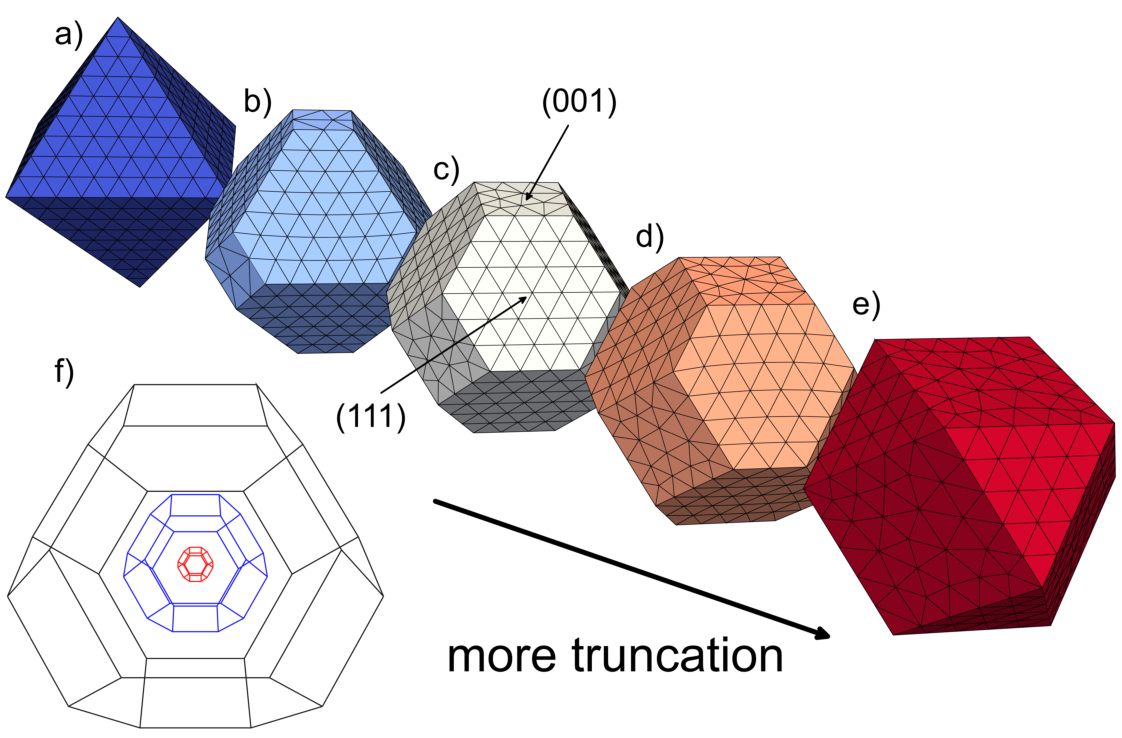
\includegraphics[width=\textwidth]{Figure_01_HR.pdf}
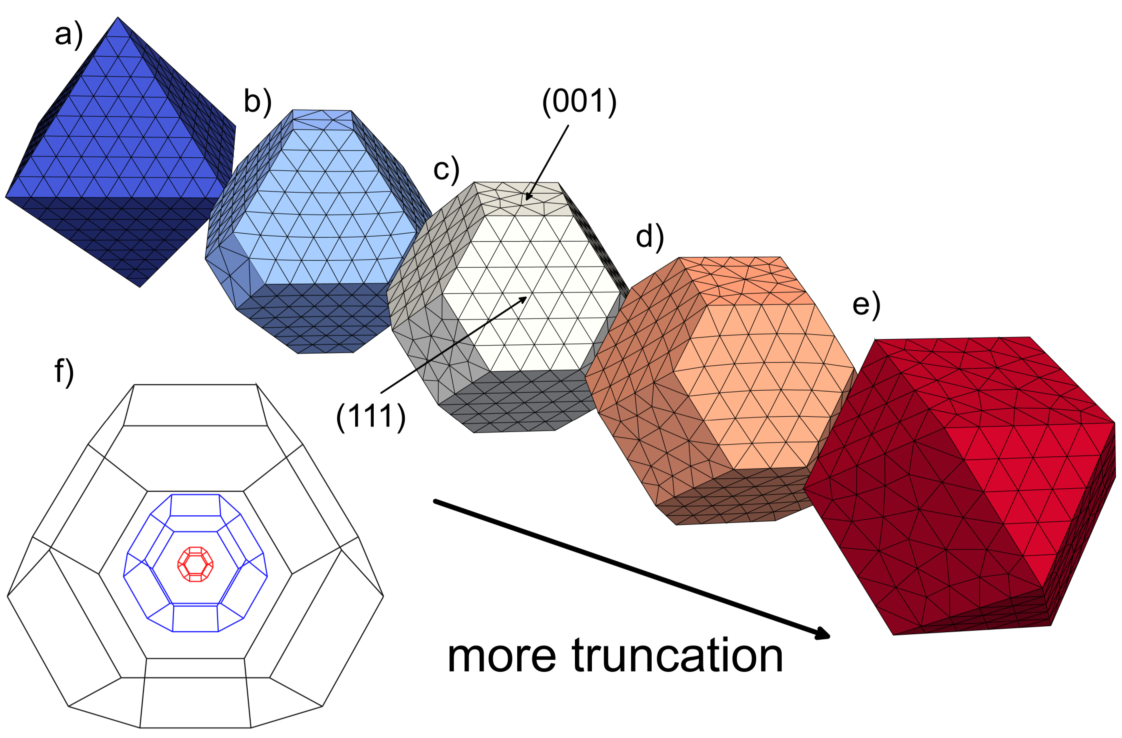
\includegraphics[width=\textwidth]{research-1/figs/Figure_01.pdf}
\caption[FE meshes of the model euhedral geometries]{FE meshes of the model euhedral geometries. From a) a regular octahedron, the rest are obtained by increasingly cutting more off the corners such that the edges of the octahedron are: b) halved (min. t. octahedron); c) reduced to a third (regular t. octahedron); d) reduced to a quarter (max. t. octahedron). e) A regular cuboctahedron is obtained by truncating to the point where the octahedron edges disappear entirely. The easy axes of magnetisation are the $<$111$>$ and the hard are the $<$001$>$, which are normal to the hexagonal $\{111\}$ and square $\{001\}$ faces, respectively, of the truncated octahedra. For a sense of scale, f) three nested regular truncated octahedra are shown with sizes 30$\nm$ (red), 120$\nm$ (blue) and 300$\nm$ (black).}
\label{fig1}
\end{figure}

\subsection{Crystal growth model}
The magnetic domain structure of a ferromagnetic nanoparticle obtained by a micromagnetic algorithm is not only a function of its mineralogy, size and shape, but also of its history. In particular, it is known that a SD particle can grow and remain SD up to a threshold size $\dmax$ after which it will become PSD \citep{Enkin1994}. (In this study we are concerned with the zero-field microstructure and properties; in this context, the onset of PSD beheaviour is marked by the formation of a single-vortex structure). If the particle then decreases its volume it will remain PSD down to a threshold $\dmin$ ($< \dmax$) below which it will become SD again. This defines a size range in which a ferromagnetic grain can be either SD or PSD dependent on its history \citep{Muxworthy2006}. This phenomenon has been modelled for the seven morphologies (Fig. \ref{fig1}) in the 30$\nm$ to 300$\nm$ size range.\par

Starting from a 30$\nm$ particle, we obtain the micromagnetic solution and extrapolate it to a larger grain. This becomes the new initial condition for which we solve and repeat, growing the particle in steps of 2$\nm$. Since a very fine incremental size step is used, much smaller than the exchange length, we can be certain that we are not missing any features from one step to the next. This process accurately models grain growth.\par

Once the particles have grown to 120$\nm$, the procedure is then reversed in decreasing steps of 2$\nm$ until the initial size of 30$\nm$ is reached. Since chemical alteration usually proceeds by alteration of the surfaces, the volume decreasing process can be thought of as a model for chemical alteration to a non-magnetic phase. This growth from 30$\nm$ to 120$\nm$ followed by the reverse process is referred to as the \textit{main loop} (ML).\par

Solutions on the size-descending curve not found on the size-increasing curve were also subject to growth; the \textit{secondary loop} (SL). The ML and SL allow us to investigate the different domain states with size, shape and history. These micromagnetic solutions were performed by numerical integration of the LLG equation (Eqn. \ref{llg}). Stable solutions at 120$\nm$, whether found on the ML or SL, were further grown up to 300$\nm$. Energy minimisation was used for calculations larger than 120$\,$nm, as integration of the LLG equation is prohibitively slow at these sizes. The parallel \textit{DUNLOP} package \citep{Nagy2016} was used to model these grain size dependencies.\par

These models overlook the effect of thermal fluctuations. However, this limitation is addressed by calculation of the relaxation times. These allow the determination of the particles domain state at a given size beyond the capabilities of standard micromagnetics.\par

\subsection{Relaxation times}
Over a sufficiently long observation time, termed the \textit{relaxation time}, a ferromagnetic particle will switch between different stable states due to thermal activation. The relaxation time is given by \citep{Neel1955}
\begin{equation}\label{neel}
\tau = \tau_0 \exp\left(E_{B}/K_{\text{B}}T\right),
\end{equation}
where $K_{\text{B}}$ is Boltzmann's constant, $T$ the temperature at which the transition occurs and $\tau_0$ the \textit{attempt time}, commonly with a value of $\roughly$10$^{-9}\,$s \citep{McNab1968}. Any transition between stable states must occur along an AMP \citep{Fabian2017}; $E_B$ is the energy barrier along such a path. When $E_B$ is of the order of the thermal energy available on a timescale of interest, a particle is in a superparamagnetic (SP) state, spontaneously switching back and forth between different SD orientations. SD grains with an energy barrier larger than $\roughly60\,K_\text{B}T$ have a relaxation time in the order of billions of years and are thus considered stable SD (SSD) reliable palaeomagnetic recorders \citep{Dunlop}. The SP--SSD threshold is therefore one of the key parameters to assess the palaeomagnetic significance of a NRM. A NEB method \citep{Fabian2017} has been implemented in the micromagnetic package \textit{MERRILL} \citep{Nagy2017} (such methods are currently unavailable in \textit{DUNLOP}) to calculate the energy barriers between the stable configurations for the (truncated) octahedral particles, from 30$\nm$ increasing in steps of 2$\nm$ until the blocking volume is reached, which is here taken to be the volume for which the relaxation time surpasses four billion years.\par

Unlike early NEB methods (as applied to magnetic systems) which approximated each particle as a single dipole \citep{Berkov1998}, here we are concerned with full micromagnetic solutions and thus, our results extend beyond SD configurations and coherent rotations. A similar method was implemented by \citet{Dittrich2002} to study the energy barriers in patterned granular media.\par
%-----------------------------------------------------

\section{Results and Discussion}
\subsection{Magnetic structure in the SD--PSD regime}\label{sd-psd}
Starting at 30$\nm$ from a randomised initial condition, all shapes relax to a SD state along an easy direction. Extrapolating onto larger grains, this state remains stable up to a threshold $\dmax$ (Figs. \ref{fig2}a, c). When the SD state solutions are grown beyond $\dmax$, they are found to relax to an easy aligned vortex (EAV) (Figs. \ref{fig2}a, d). For all shapes, this vortex configuration is stable up to 120$\nm$. On reversal, the EAV is stable down to a threshold $d_{\text{EH}}$ (Fig. \ref{fig2}a). Below $d_{\text{EH}}$, the EAV goes to a hard-aligned vortex (HAV) preserving its chirality (Figs. \ref{fig2}a, e). Further decreasing the volume, the HAV is stable down to $\dmin$ and below that, the HAV relaxes back to SD (Fig. \ref{fig2}a). This general behaviour on the ML is referred to as Type 1 (Figs. \ref{fig2}a, \ref{fig3}a, e, g, k), for which we introduce the notation:
\begin{equation}\label{type1}
\text{T}_1=\underbrace{\left(\text{SD}_{30}^{\dmax}\rightarrow\text{EAV}_{\dmax}^{120}\right)_{\rightarrow}}_\text{growth part} +
\underbrace{\left(\text{EAV}_{120}^{d_{\text{EH}}}\rightarrow\text{HAV}_{d_{\text{EH}}}^{\dmin}\rightarrow\text{SD}_{\dmin}^{30}\right)_{\leftarrow}}_\text{volume-decreasing part},
\end{equation}
with $30\,\text{nm}<\dmin<d_{\text{EH}}<\dmax<120\,\text{nm}$.\par
\begin{figure}
\centering
%\includegraphics[width=\textwidth]{Figure_02_HR.pdf}
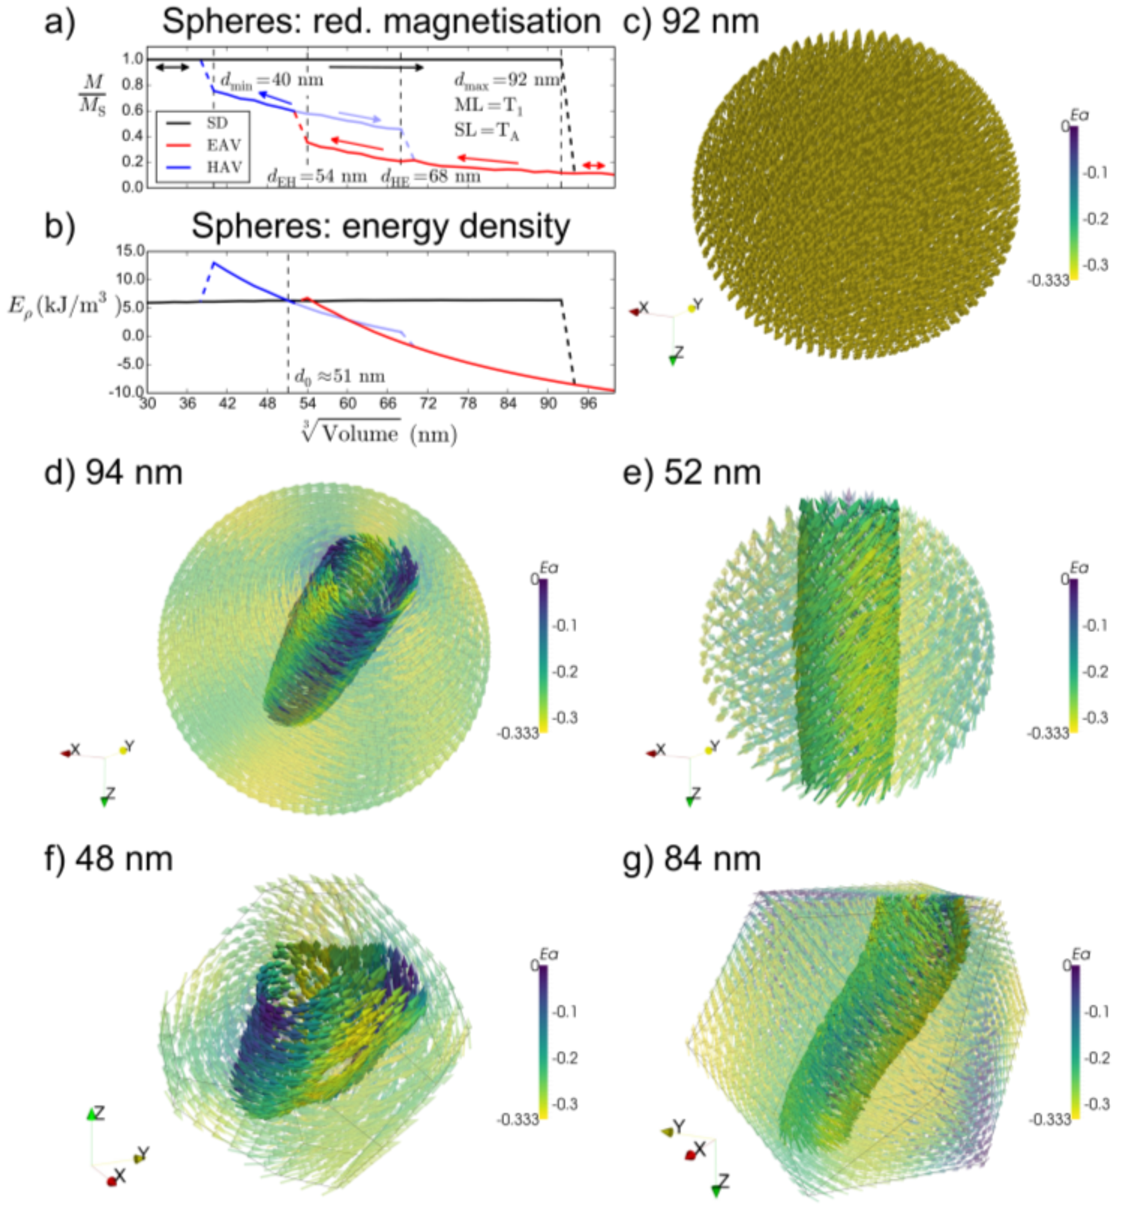
\includegraphics[width=\textwidth]{research-1/figs/Figure_02.pdf}
\caption[Micromagnetic structures of spheres and intermediate-aligned vortex states]{Micromagnetic structures of spheres and intermediate-aligned vortex states. Reduced magnetisation (a) and energy density (b) against size. The SD [$\bar{1}\bar{1}\bar{1}$] state is numerically stable up to $\dmax=92\,\text{nm}$ (c). Growing this solution to a 94$\nm$ grain it is found to relax to a [$\bar{1}\bar{1}\bar{1}$] EAV (d), stable up to 120$\nm$. The EAV is then interpolated into smaller grains, stable down to $d_\text{EH}=54\,\text{nm}$ (a). At 52$\nm$ the EAV goes to a [00$\bar{1}$] HAV (e), stable down to $\dmin=40\,\text{nm}$. At 38$\nm$, the solution relaxes to the original SD state (a). This sequence is referred to as a Type 1 \textit{main loop} (ML). Growth of the HAV from 52$\nm$ forms the Type A \textit{secondary loop} (SL): the HAV is found to be stable up to $d_{\text{HE}}=68\,\text{nm}$ (a) and to realign with the easy direction at 70$\nm$. Vortex states can not only be easy or hard-aligned, but also $<$011$>$ intermediate-aligned vortices (IAVs) (f) and distorted IAV configurations (dIAV) (g). MLs in which IAVs are found are referred to as Type 2. Colour represents the MCA energy normalised by $|K_1|$. The vortex cores are highlighted by obtaining a helicity ($K=\boldsymbol{m}\cdot\nabla\times\boldsymbol{m}$) isosurface and reducing the opacity of the rest of the arrows.}
\label{fig2}
\end{figure}

Another sequence was observed. On the size-descending curve, the EAV is stable down to a threshold $d_{\text{EI}}$ below which the EAV goes to a $<$011$>$ intermediate-aligned vortex (IAV) (Figs. \ref{fig2}f, g), stable down to $d_{\text{IH}}$. Below that, the IAV goes to a HAV which remains down to $\dmin$. Finally, below $\dmin$ the HAV relaxes back to SD. This ML behaviour is referred to as Type 2 (Figs. \ref{fig3}c, i), with the formula:
\begin{equation}\label{type2}
\text{T}_2=\underbrace{\left(\text{SD}_{30}^{\dmax}\rightarrow\text{EAV}_{\dmax}^{120}\right)_{\rightarrow}}_\text{growth part} +
\underbrace{\left(\text{EAV}_{120}^{d_{\text{EI}}}\rightarrow\text{IAV}_{d_{\text{EI}}}^{d_{\text{IH}}}\rightarrow\text{HAV}_{d_{\text{IH}}}^{\dmin}\rightarrow\text{SD}_{\dmin}^{30}\right)_{\leftarrow}}_\text{volume-decreasing part},
\end{equation}
with $30\,\text{nm}<\dmin<d_{\text{IH}}<d_{\text{EI}}<\dmax<120\,\text{nm}$.\par

Growth of the vortex configurations found on the size-descending curve (HAVs, IAVs) forms the SL. When the ML is Type 1, the HAV is grown up to a threshold $d_\text{HE}$ beyond which it realigns with an easy direction (Fig. \ref{fig2}a). When the ML is Type 2, the HAV goes to either an EAV (Fig. \ref{fig3}c) or to the IAV it nucleated from (Fig. \ref{fig3}i). When the IAV is grown beyond a threshold $d_\text{IE}$ it realigns with an easy direction (Fig. \ref{fig3}c). This behaviour on the SL is referred to as Type A (Fig. \ref{fig2}a, \ref{fig3}c, e, g), with the general formula (in the case of growth of the HAV and realignment to an EAV):
\begin{equation}\label{typeA}
\text{T}_{\text{A}}=\underbrace{\left(\text{HAV}_{d_{\text{EH}}}^{d_{\text{HE}}}\rightarrow\text{EAV}_{d_{\text{HE}}}^{120}\right)_{\rightarrow}}_\text{secondary growth part}.
\end{equation}
There is also the possibility that the HAV/IAV is stable up to 120$\nm$. This SL is a Type B (Fig. \ref{fig3}a, i, k), with the general formula (in the case of growth of the HAV):
\begin{equation}\label{typeB}
\text{T}_{\text{B}}=\underbrace{\left(\text{HAV}_{d_{\text{EH}}}^{120}\right)_{\rightarrow}}_\text{secondary growth part}.
\end{equation}
\begin{figure}
\centering
%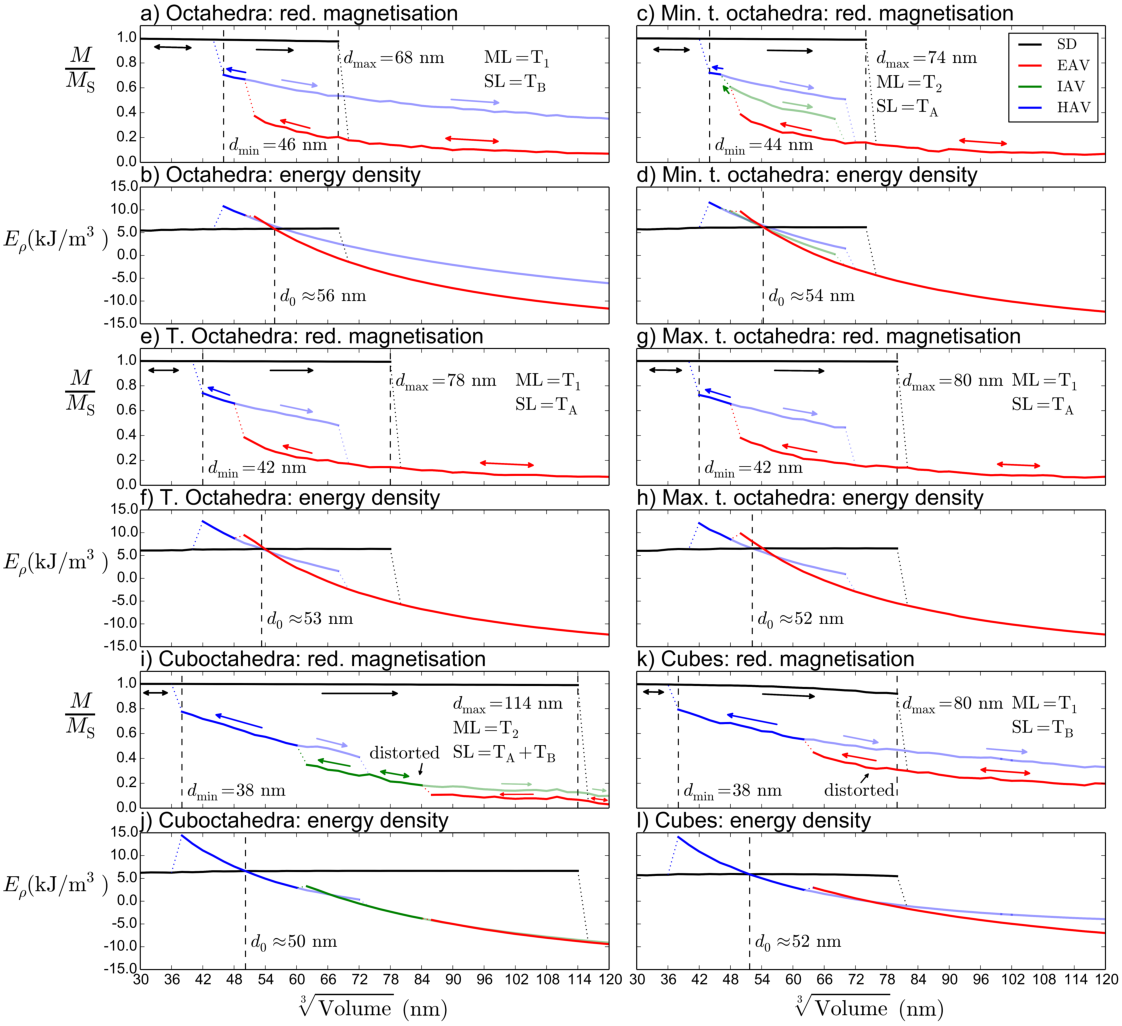
\includegraphics[width=\textwidth]{Figure_03_HR.pdf}
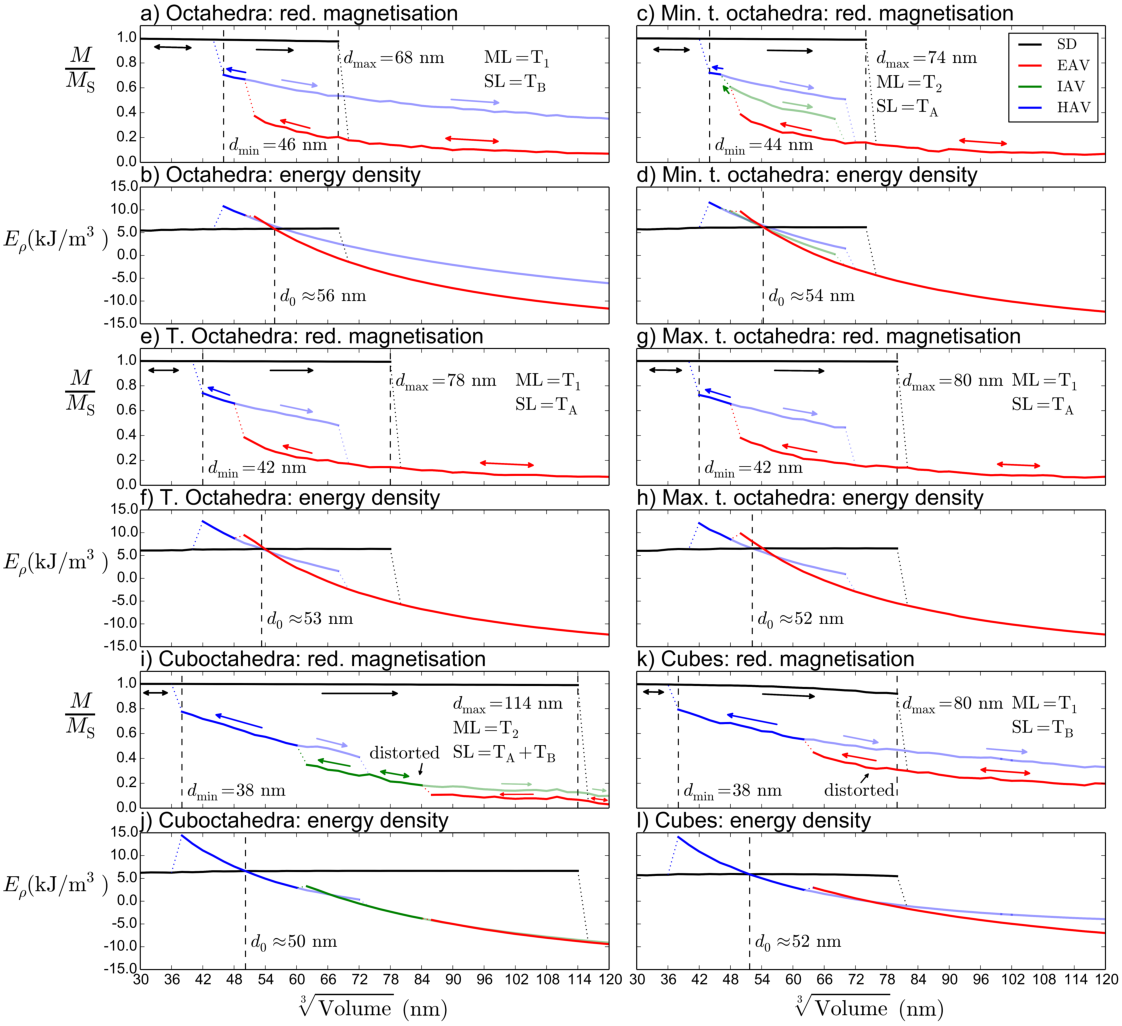
\includegraphics[width=\textwidth]{research-1/figs/Figure_03.pdf}
\caption[Domain states and energies in the SD--PSD transition regime]{Domain states and energies in the SD--PSD transition regime. Reduced magnetisation (a, c, e, g, i, k) and energy density (b, d, f, h, j, l) against size. All shapes relax to an easy aligned SD state at 30 nm from a randomised initial condition. The SD state is numerically stable up to $\dmax$ (black lines). Growth beyond $\dmax$ results in the magnetisation relaxing to an EAV, stable up to 120$\nm$ (red lines). The solution is then interpolated into smaller grains. This forms the \textit{main loop} (ML) (opaque lines). The EAV is stable down to a threshold beyond which a HAV is nucleated on the size-descending curve. The HAV is stable down to $\dmin$, below which it relaxes to a SD state. This is a Type 1 ML (a, e, g, k). When the EAV goes through an IAV (green lines) before going to the HAV configuration the ML is Type 2 (c, i). Growth of the HAVs and IAVs found on the size-descending curve forms the \textit{secondary loop} (SL) (translucent lines). When these realign with the EAV or with the vortex state they nucleated from the SL is Type A (c, e, g, i (translucent blue line)). When they are stable up to 120$\nm$ the SL is Type B (a, i (translucent green line), k).}
\label{fig3}
\end{figure}

\subsubsection{Spheres}
Fig. \ref{fig2}a shows the reduced magnetisation and Fig. \ref{fig2}b the energy density (against size) for the spherical shapes. Spheres showed a Type 1 ML (Eq. \ref{type1}), with a specific formula:
\begin{equation}
\text{ML}_{\text{sph.}}=\left(\text{SD}_{30}^{92}\rightarrow\text{EAV}_{94}^{120}\right)_{\rightarrow} + \\
\left(\text{EAV}_{120}^{54}\rightarrow\text{HAV}_{52}^{40}\rightarrow\text{SD}_{38}^{30}\right)_{\leftarrow}.
\end{equation}
The SD state at $\dmax=92\,\text{nm}$ and the EAV at 94$\nm$ are shown in Figs. \ref{fig2}c--d. The SL is formed by growing the HAV found at 52$\nm$ (Fig. \ref{fig2}e). This is a Type A SL (Eq. \ref{typeA}), with formula:
\begin{equation}
\text{SL}_{\text{sph.}}=\left(\text{HAV}_{52}^{68}\rightarrow\text{EAV}_{70}^{120}\right)_{\rightarrow}.
\end{equation}
\par

\subsubsection{Octahedra and truncated octahedra}
Fig. \ref{fig3} shows the reduced magnetisation and energy density plots for the rest of the shapes. The octahedra (Figs. \ref{fig3}a--b) showed a Type 1 ML (Eq. \ref{type1}), specifically:
\begin{equation}
\text{ML}_{\text{oct.}}=\left(\text{SD}_{30}^{68}\rightarrow\text{EAV}_{70}^{120}\right)_{\rightarrow} + \\
\left(\text{EAV}_{120}^{52}\rightarrow\text{HAV}_{50}^{46}\rightarrow\text{SD}_{44}^{30}\right)_{\leftarrow}.
\end{equation}
The SD state at $\dmax=68\,\text{nm}$ (Fig. \ref{fig4}a) shows significant flowering{\textemdash}deflection of the magnetisation onto edges and vertices. The EAV nucleated at 70$\nm$ is shown in Fig. \ref{fig4}b. Growth of the HAV nucleated at 50$\nm$ (Fig. \ref{fig4}c) showed a Type B SL (Eq. \ref{typeB}), \textit{i.e.,} the HAV was found to be stable up to 120$\nm$,
\begin{equation}
\text{SL}_{\text{oct.}}=\left(\text{HAV}_{50}^{120}\right)_{\rightarrow}.
\end{equation}

The minimally truncated octahedra (Figs. \ref{fig3}c--d) showed a Type 2 ML (Eq. \ref{type2}):
\begin{equation}
\text{ML}_{\text{t.oct.}}^{\text{min.}}=\left(\text{SD}_{30}^{74}\rightarrow\text{EAV}_{76}^{120}\right)_{\rightarrow} + \\
 \left(\text{EAV}_{120}^{50}\rightarrow\text{IAV}_{48}^{48}\rightarrow\text{HAV}_{46}^{44}\rightarrow\text{SD}_{42}^{30}\right)_{\leftarrow}.
\end{equation}
The SD state shows greater stability and less flowering at $\dmax=74\,\text{nm}$ (Fig. \ref{fig4}d) than for the octahedra, before relaxing to an EAV at 76$\nm$ (Fig. \ref{fig4}e). Growth of both the IAV from 48$\nm$ (Fig. \ref{fig2}f) and HAV from 46$\nm$ (Fig. \ref{fig4}f) forms the composite SL. Both showed a Type A SL (Eq. \ref{typeA}), specifically:
\begin{equation}
\text{SL}_{\text{t.oct.}}^{\text{min.}}=\left(\text{IAV}_{48}^{68}\rightarrow\text{EAV}_{70}^{120}\right)_{\rightarrow} + \left(\text{HAV}_{56}^{70}\rightarrow\text{EAV}_{72}^{120}\right)_{\rightarrow}.
\end{equation}\par

The next two degrees of truncation, the regular truncated octahedra (Figs. \ref{fig3}e--f) and the maximally truncated octahedra (Figs. \ref{fig3}g--h), both showed Type 1 MLs (Eq. \ref{type1}):
\begin{equation}
\text{ML}_{\text{t.oct.}}^{\text{reg.}}=\left(\text{SD}_{30}^{78}\rightarrow\text{EAV}_{80}^{120}\right)_{\rightarrow} + \\
\left(\text{EAV}_{120}^{50}\rightarrow\text{HAV}_{48}^{42}\rightarrow\text{SD}_{40}^{30}\right)_{\leftarrow};
\end{equation}
and
\begin{equation}
\text{ML}_{\text{t.oct.}}^{\text{max.}}=\left(\text{SD}_{30}^{80}\rightarrow\text{EAV}_{82}^{120}\right)_{\rightarrow} + \\
\left(\text{EAV}_{120}^{48}\rightarrow\text{HAV}_{46}^{42}\rightarrow\text{SD}_{40}^{30}\right)_{\leftarrow}.
\end{equation}
The SD states show increasing stability and less flowering (Figs. \ref{fig4}g, \ref{fig5}a). The EAVs at 80$\nm$ and 82$\nm$ are shown in Figs. \ref{fig4}h, \ref{fig5}b. Growth of the HAVs nucleated at 48$\nm$ (Fig. \ref{fig4}i) and at 46$\nm$ (Fig. \ref{fig5}c) showed the SL was Type A (Eq. \ref{typeA}) for both shapes:
\begin{equation}
\text{SL}_{\text{t.oct.}}^{\text{reg.}}=\left(\text{HAV}_{48}^{68}\rightarrow\text{EAV}_{70}^{120}\right)_{\rightarrow};
\end{equation}
and
\begin{equation}
\text{SL}_{\text{t.oct.}}^{\text{max.}}=\left(\text{HAV}_{46}^{70}\rightarrow\text{EAV}_{72}^{120}\right)_{\rightarrow}.
\end{equation}
\begin{figure}
\centering
%\includegraphics[width=\textwidth]{Figure_04_HR.pdf}
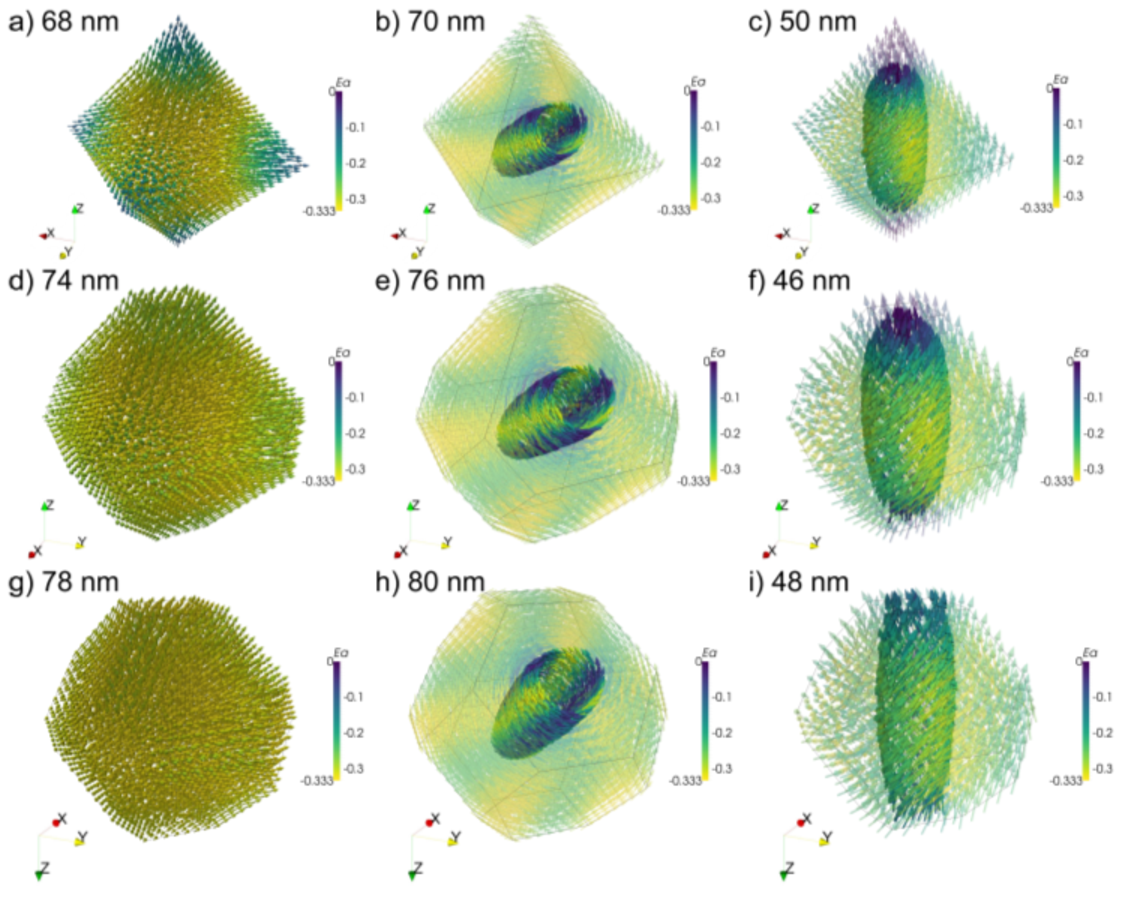
\includegraphics[width=\textwidth]{research-1/figs/Figure_04.pdf}
\caption[Micromagnetic structures of octahedra, minimally truncated octahedra and regular truncated octahedra]{Micromagnetic structures of octahedra, minimally truncated octahedra and regular truncated octahedra. Left column (a, d, g) shows the largest SD solutions at $\dmax$, obtained by interpolating from solutions for smaller grains starting at 30$\nm$. On interpolating to a grain 2$\nm$ larger, the structure relaxes to an EAV (b, e, h), stable up to 120$\nm$. From 120$\nm$ interpolation is carried out into smaller grains. Eventually the vortex aligns with a hard direction (c, f, i) which is stable down to $\dmin$ after which the solution becomes SD again down to 30$\nm$. Top row (a, b, c) shows the structures for the octahedra; center row (d, e, f) for the minimally truncated octahedra and bottom row (g, h, i) for the regular truncated octahedra. Colour represents the MCA energy normalised by $|K_1|$.}
\label{fig4}
\end{figure}

\subsubsection{Cuboctahedra}
The cuboctahedra (Figs. \ref{fig3}i--j) showed a Type 2 ML (Eq. \ref{type2}). The PSD state nucleated on the size-descending curve from the EAV is a distorted IAV (dIAV){\textemdash}a sort of mixed state with the vortex mostly aligned with the [0$\bar{1}$$\bar{1}$] direction and the ends of the vortex deflecting to a hard direction. The ML then has a formula:
\begin{equation}
\text{ML}_{\text{oct.}}^{\text{cub}}=\left(\text{SD}_{30}^{114}\rightarrow\text{EAV}_{116}^{120}\right)_{\rightarrow} + \\
 \left(\text{EAV}_{120}^{86}\rightarrow\text{dIAV}_{84}^{62}\rightarrow\text{HAV}_{60}^{38}\rightarrow\text{SD}_{36}^{30}\right)_{\leftarrow}.
\end{equation}
The SD state is more stable, with $\dmax$ increasing to $\dmax=114\,\text{nm}$ (Fig. \ref{fig5}d) before relaxing to an EAV at 116$\nm$ (Fig. \ref{fig5}e). Growth of the HAV from 60$\nm$ (Fig. \ref{fig5}f) shows a Type A SL (Eq. \ref{typeA}), with the HAV going to the dIAV it nucleated from. The dIAV (Fig. \ref{fig2}f) instead shows a Type B SL. The SL is then:
\begin{equation}
\text{SL}_{\text{oct.}}^{\text{cub}}=\left(\text{HAV}_{60}^{72}\rightarrow\text{dIAV}_{74}^{120}\right)_{\rightarrow} + \left(\text{dIAV}_{84}^{120}\right)_{\rightarrow}.
\end{equation}
\par

\subsubsection{Cubes}
The cubes (Figs. \ref{fig3}k--l) showed a Type 1 ML (Eq. \ref{type1}). The EAV nucleated from the SD state is a distorted EAV (dEAV). The dEAV mostly aligns with an easy direction, but its ends deflect from the vertices to a hard direction, attaching to opposite faces. The ML is then:
\begin{equation}
\text{ML}_{\text{cube}}=\left(\text{SD}_{30}^{80}\rightarrow\text{dEAV}_{82}^{120}\right)_{\rightarrow} + \\
\left(\text{dEAV}_{120}^{64}\rightarrow\text{HAV}_{62}^{38}\rightarrow\text{SD}_{36}^{30}\right)_{\leftarrow}.
\end{equation}
The SD state at $\dmax=80\,\text{nm}$ is largely flowered (Fig. \ref{fig5}g). The dEAV initially nucleated at 82$\nm$ (Fig. \ref{fig5}h) could also be interpreted as a distorted HAV. However, the alignment of such state with an easy direction becomes more obvious for larger cubes. Growth of the HAV from 62$\nm$ (Fig. \ref{fig5}i) results in a Type B SL:
\begin{equation}
\text{SL}_{\text{cube}}=\left(\text{HAV}_{62}^{120}\right)_{\rightarrow}.
\end{equation}
\begin{figure}
\centering
%\includegraphics[width=\textwidth]{Figure_05_HR.pdf}
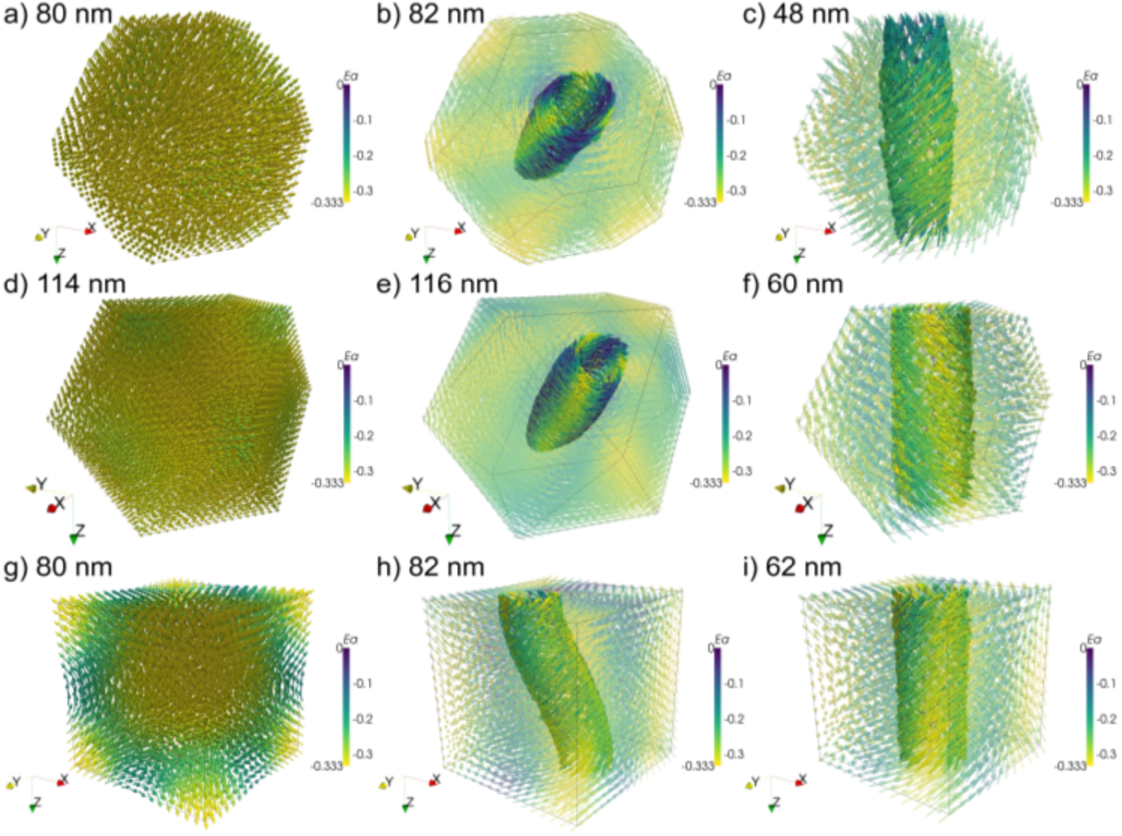
\includegraphics[width=\textwidth]{research-1/figs/Figure_05.pdf}
\caption[Micromagnetic structures of maximally truncated octahedra, cuboctahedra and cubes]{Micromagnetic structures of maximally truncated octahedra, cuboctahedra and cubes. Left column (a, d, g) shows the largest SD solutions at $\dmax$, obtained by interpolating from solutions for smaller grains starting at 30$\nm$. On interpolating to a grain 2$\nm$ larger, the structures relax to an EAV (b, e) or a distorted EAV (h) which are stable up to 120$\nm$. From 120$\nm$ interpolation is carried out into smaller grains. Eventually the vortex aligns with a hard direction (c, f, i), stable down to $\dmin$ after which the solution becomes SD again down to 30$\nm$. Top row (a, b, c) shows the structures for the maximally truncated octahedra; center row (d, e, f) for the cuboctahedra and bottom row (g, h, i) for the cubes. Colour represents the MCA energy normalised by $|K_1|$.}
\label{fig5}
\end{figure}

\subsubsection{Discussion}
The values for $\dmax$ of the spheres are significantly larger than those found for the euhedral shapes (except for the cuboctahedra which have an anomalously large value), perhaps due to the absence of corners to act as nucleation points. Truncation of the octahedral particles increases the (numerical) stability of the SD solutions which is expressed as the increase in $\dmax$ from 68$\nm$ for the octahedra (Fig. \ref{fig3}a) to 114$\nm$ for the cuboctahedra (Fig. \ref{fig3}i) (Table \ref{table1}). A less pronounced effect is the decrease of $\dmin$ with truncation from 46$\nm$ for the octahedra to 38$\nm$ for the cuboctahedra (Table \ref{table1}). HAVs are more (numerically) stable at smaller sizes the more truncated the particle is. This is due to the large stray field energy created by a vortex pointing towards a vertex. It is energetically favourable for a vortex to attach its ends to flat surfaces large enough to accomodate its core. This is seen in the distortion of the vortex structures shown in Figs. \ref{fig2}g, \ref{fig5}h. These avoid the production of large stray fields by attaching their ends to grain faces, at the cost of anisotropy and exchange energies needed to distort the otherwise straight structures of the vortices.\par
\begin{table}[ht]
\centering
\begin{tabular}{| l || c | c | c | c | c | c | c |}
\hline
       & main loop & $\dmax$ & $d_\text{EH}$ & $d_\text{EI}$ & $d_\text{IH}$ & $\dmin$ & $d_0$ \\
\hline
Spheres & T$_1$ & 92 & 54 & N/A & N/A & 40 & 51 \\
\hline
Octahedra & T$_1$ & 68 & 52 & N/A & N/A & 46 & 56 \\
\hline
Min. t. octahedra & T$_2$ & 74 & N/A & 50 & 48 & 44 & 54 \\
\hline
T. octahedra & T$_1$ & 78 & 50 & N/A & N/A & 42 & 53 \\
\hline
Max. t. octahedra & T$_1$ & 80 & 48 & N/A & N/A & 42 & 52 \\
\hline
Cuboctahedra & T$_2$ & 114 & N/A & 86 & 62 & 38 & 50 \\
\hline
Cubes & T$_1$ & 80 & 64 & N/A & N/A & 38 & 52 \\
\hline
\end{tabular}
\caption[Critical sizes for all shapes]{Critical sizes for all shapes. All sizes in nm. $d_0$, $\dmin$ decrease with truncation while $\dmax$ increases.}
\label{table1}
\end{table}

The energy plots (Figs. \ref{fig2}b, \ref{fig3}b, d, f, h, j, l) show the SD energy density is fairly constant with size for all shapes. For the octahedra, the intersection of the EAV and HAV energy curves occurs above the SD curve. This means that it is then the EAV energy curve which first intersects the SD curve at $d_0$ and thus this PSD state becomes the GEM thereon (Fig. \ref{fig3}b). With truncation, this intersection moves closer to the SD curve as can be seen in Fig. \ref{fig3}d in which all the different PSD states (EAV, IAV and HAV) and the SD energy curves meet at roughly the same point. Further truncation causes this intersection to eventually occur below the SD energy curve. This creates a narrow range of sizes for which the HAV is the lowest energy state (Figs. \ref{fig3}f, h). Completely truncated, the cuboctahedra show a \textit{split} of this intersection into distinct crossings of the HAV/IAV and IAV/EAV energy curves (Fig. \ref{fig3}i, compare with Fig. \ref{fig3}d), creating a broad range of sizes, from $\roughly$50$\nm$ to $\roughly$66$\nm$, for which the HAV has the lowest energy. A range for which the HAV has the lowest energy was also found for spheres and cubes. The overall effect of truncation on $d_0$ is to decrease this threshold (Table \ref{table1}).\par

For the cubes we found $\dmax=80\,\text{nm}$, much smaller than the value of 107$\nm$ obtained by \citet{Muxworthy2013}. We found $\dmin=38\,\text{nm}$, in agreement with the value by \citet{Muxworthy2013}. We found the intersection of the SD and HAV energy curves $d_0\approx 52\,\text{nm}$ (Fig. \ref{fig3}l), lower than the value of 58$\nm$ by \citet{Muxworthy2013}. Modelling the ML for cubes with the $M_\text{S}$ value used by \citet{Muxworthy2013} we obtained $\dmax=92\,\text{nm}$, $\dmin=42\,\text{nm}$ smaller and larger, respectively, than the values by \citet{Muxworthy2013}. The differences in $\dmax$, $\dmin$ can be due to \citet{Muxworthy2013} using a FD method as opposed to a FEM used here. However, excellent agreement of $d_0\approx 60\,\text{nm}$ was found with the value of 58$\nm$ by \citet{Muxworthy2013}. The difference between $d_0$ obtained with the different $M_\text{S}$ is significant as it is larger than the exchange length and thus, unlikely to be an effect of discretisation.\par

\subsection{Identifying the PSD--MD transition}
Unlike fine SD grains, bulk ferromagnetic materials can possess a (roughly) null net magnetisation. This is because bulk ferromagnets, in their lowest energy state, have a multi-domain (MD) magnetic structure \citep{Dunlop}. MD structure is characterised by the coexistence of multiple magnetic domains: small regions saturated in different easy directions and separated by narrow planar regions called domain walls where the magnetisation vector transforms continuously from the direction of one domain to that of its neighbour. Near the surface of a bulk sample the magnetic domains lie in directions parallel to the surfaces, which do not necessarily coincide with the magnetocrystalline easy axes; these are called \textit{closure domains} as they enclose the magnetic flux. Then, MD grains minimise the stray field energy at the expense of exchange and MCA energies associated with the domain walls and closure domains. This balance becomes more energetically favourable as a particle grows. To identify a plausible PSD--MD transition, EAV states found to be stable at 120$\nm$ were further grown up to 300$\nm$ in steps of 2$\nm$.\par

\subsubsection{Growth of EAVs}
The octahedron EAV (Fig. \ref{fig4}b) was found to remain stable up to 300$\nm${\textemdash}as was the case for the EAVs for all shapes. However, although the overall structure is preserved as the grain grows, there is a gradual, continuous transformation towards MD structure. As the crystal becomes larger, the vortex core (the cylindrical region encompassing the highest helicity $K=\boldsymbol{m}\cdot\nabla\times\boldsymbol{m}$) width remains the same. The regions radially far from the core become screened from its influence and more influenced by the effects of MCA, giving way to six ever larger expanses of the grain that become magnetised along easy axes. The sections with higher MCA energy become increasingly narrower, more planar and confined between the easy-aligned regions. With further growth, the regions close to the edges become magnetised along the edges thus completing a picture of MD structure: magnetic domains magnetised along easy directions (Fig. \ref{fig6}a); flat, narrow magnetic domain walls dividing these and closure domains formed along edges of the body (Fig. \ref{fig6}b). The spheres (not shown) show this same general behaviour of formation of magnetic domains and domain walls, but without the formation of closure domains as there are no edges to nucleate these type of domains.\par

At 300$\nm$, the regular truncated octahedron shows the same basic structure as the 300$\nm$ octahedron except for the widening of the domain walls as they approach the square $\{$001$\}$ faces (Figs. \ref{fig6}c--d). Completely truncated, the cuboctahedra have a somewhat different structure. In the 300$\nm$ cuboctahedron solution the domain walls have become so wide as they draw closer to the square faces that they engulf three of the magnetic domains (Fig. \ref{fig6}e), and hard-aligned N\'eel walls appear which are visible as blue streaks on the square faces (Fig. \ref{fig6}f).
\begin{figure}
\centering
%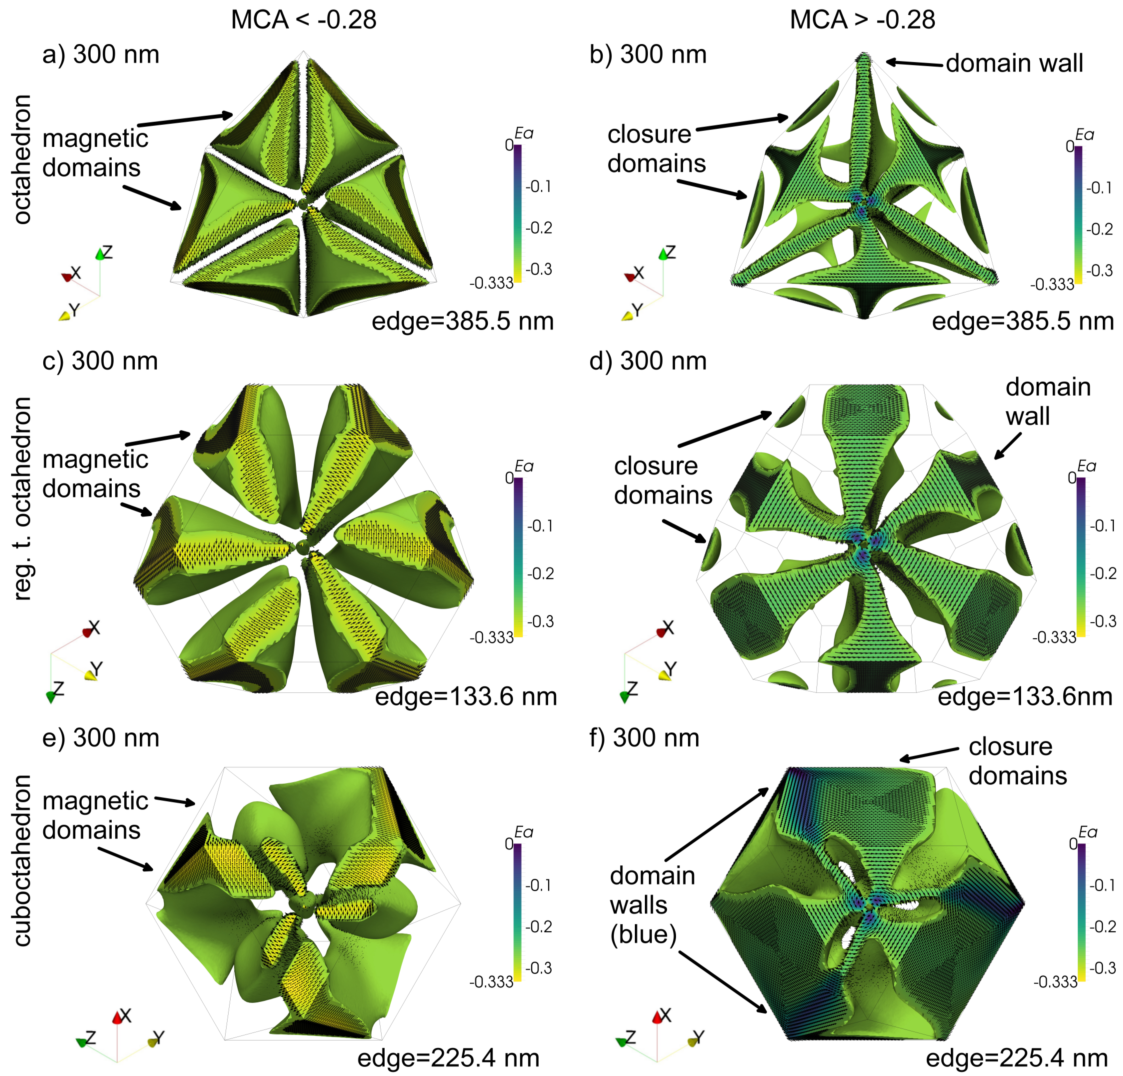
\includegraphics[width=\textwidth]{Figure_06_HR.pdf}
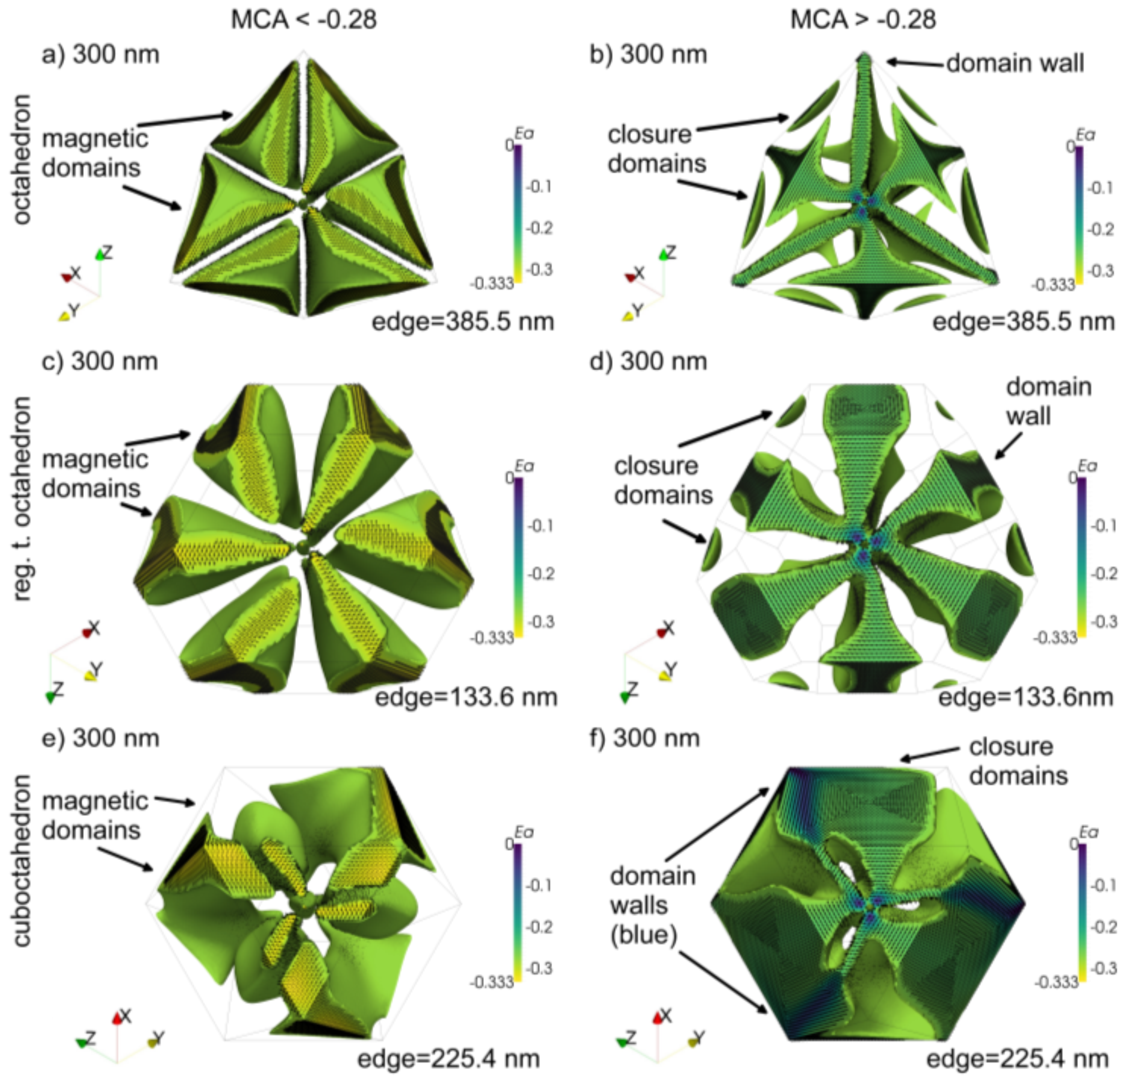
\includegraphics[width=\textwidth]{research-1/figs/Figure_06.pdf}
\caption[MD formation by easy aligned vortices]{MD formation by easy aligned vortices. From the solutions obtained by growing the 120$\nm$ EAVs up to 300$\nm$, the mesh nodes with MCA energy $<$-0.28 (normalised by $|K_1|$) are shown in the left column (a, c, e). These are regions which deviate from an easy axis alignment by less than $\roughly$15$^{\circ}$. The complement is shown in the right column: the regions with moderate to high ($>$-0.28) MCA energy (b, d, f). In the octahedron, there form six large magnetic domains filling up most of the volume (a) and narrow, flat regions acting as domain walls and small wedge-like regions formed along the edges interpreted as closure domains (b). The regular truncated octahedron EAV grown up to 300$\nm$ shows the same pattern: large magnetic domains with low MCA energy occupy most of the volume (c); the effect of truncation (and consequent creation of $\{001\}$ surfaces) is to widen the domain walls as they approach the surfaces as this reduces the stray field energy (d). Closure domains along the edges are still pronounced (d). Fully truncated, the effect on the structure of the cuboctahedron EAV grown to 300$\nm$ is to reduce the proportion of the volume occupied by magnetic domains (e). The domain walls are so wide close to the surfaces that they engulf three of the domains, while also hard-aligned N\'eel walls are formed as seen from the blue streaks on the surface (f). Colour represents the MCA energy normalised by $|K_1|$.}
\label{fig6}
\end{figure}

\subsubsection{Discussion}
A tentative mechanism for a PSD--MD transition has been identified. This proceeds by a gradual formation of magnetic domains, domain walls and closure domains `seeded' by the vortex structures nucleated in the SD--PSD transition regime. However, this transition is more obvious for the octahedra than the truncated octahedra and cuboctahedra.\par

Since our models do not account for the effects of thermal fluctuations, the stability of the solutions is only numerical, e.g., the energy landscape of a micromagnetic solution is somewhat flat in the vicinity of the solution, thus small numerical perturbations can be insufficient for a micromagnetic algorithm to drive the solution to a new local energy/torque minimum depending on the sensitivity or control parameters of the algorithm. We find for the octahedra and the cuboctahedra two solutions for each morphology up to 300$\nm$ (Figs. \ref{fig3}a, e). Although the EAVs for both have the lowest energies, this leaves open the question of whether we can expect to find metastable grains with the higher energy structures. Likewise, in Section \ref{sd-psd} we find that grains remain SD beyond $d_0$. In theory, a particle can remain in a metastable SD state beyond this threshold if the energy barrier separating the SD from the PSD state is higher than the thermal energy available. Knowledge of the energy barriers near the SD--PSD transition is needed to answer these questions.\par

\subsection{Energy barriers and blocking volumes}
A nudged elastic-band (NEB) method \citep{Fabian2017} was implemented for the calculation of the energy barriers at room temperature as a function of size and shape for the (truncated) octahedral morphologies. To calculate the energy barrier for a given shape and size we obtain many solutions from randomised initial conditions. From this set of solutions the state with the lowest energy is identified. For the smaller particles we expect the GEM to be SD and for larger grains PSD. Once the GEM has been identified from the set of initial solutions, two appropriate solutions must be chosen to calculate the action-minimising path (AMP) between them and thus the energy barrier.\par

When the GEM is a $<$111$>$-aligned SD state, the pair of appropriate solutions are magnetised normal to contiguous $\{$111$\}$ faces. Above $d_0$ the GEM is usually a HAV, then, the paths to test are between vortices at 90$^{\circ}$ from each other, e.g., between [100] and [001] vortices. For some shapes the GEM is a distorted vortex, for these, it is important to calculate several paths between different configurations to find the transition with the lowest energy barrier. At larger sizes, for all shapes the GEM is an EAV, this means that the paths to calculate are between vortices pointing towards contiguous $\{$111$\}$ faces, much like for SD particles. For all PSD to PSD transitions the vortices must have the same chirality as a change produces prohibitively large energy barriers one to two orders of magnitude larger than the AMP barrier and thus we can neglect the possibility of such transitions. It is not necessary to calculate the energy barriers for transitions other than the ones with the lowest energy as these dominate the behaviour and higher energy transitions usually proceed via lower energy ones \citep{Nagy2017}. For perfectly regular, equant grains as those modelled in this study, the lowest energy transition is degenerate and so, the relaxation time has to be divided by three (for the three distinct degenerate paths).\par

\subsubsection{Octahedra and truncated octahedra}
Fig. \ref{fig7} shows three examples of transitions for the regular truncated octahedra which were found to be typical for all the (truncated) octahedra, but for the cuboctahedra. At the smaller sizes (Fig. \ref{fig7}, left column) the transition is from SD to SD via coherent rotation. The energy along such a path is plotted in Fig. \ref{fig7}a; the energy barrier is the difference between the easy (Figs. \ref{fig7}d, j) and intermediate-aligned SD (Fig. \ref{fig7}g) energies. The energy barrier for such transitions, for all shapes, is quite low, with relaxation times from a few microseconds to a few days for the largest of these. A few nanometers before the SD--PSD transition the AMP is not a coherent rotation, but a transition via a curling mode (Fig. \ref{fig7}, center column). The energy barrier is also the difference between the easy and intermediate-aligned SD energies.\par

Once the GEM is an EAV, the transitions are between isochiral EAVs directed towards contiguous $\{$111$\}$ faces (Fig. \ref{fig7}, right column). The transition is a structured rotation of the vortex, through an IAV (Fig. \ref{fig7}i), which maintains its overall shape along the path. The energy along such paths is a double-bump where the IAV sits in a shallow local energy minimum (LEM). This means that the energy barrier is not the difference between the EAV and IAV energies. Rather, it is given by the barrier separating the EAV from the IAV. However, with increasing size the IAV LEM becomes more shallow and thus the energy barrier is better approximated by the difference between the EAV and IAV energies{\textemdash}at 64$\nm$ the IAV LEM is so shallow that the double-bump feature becomes flattened (Fig. \ref{fig7}c). In general, the PSD to PSD transitions are very similar to coherent rotations between SD states in that they are structured rotations of the vortex core. The left column of Video 1 (supplementary material) shows these typical transitions.
\begin{figure}
\centering
%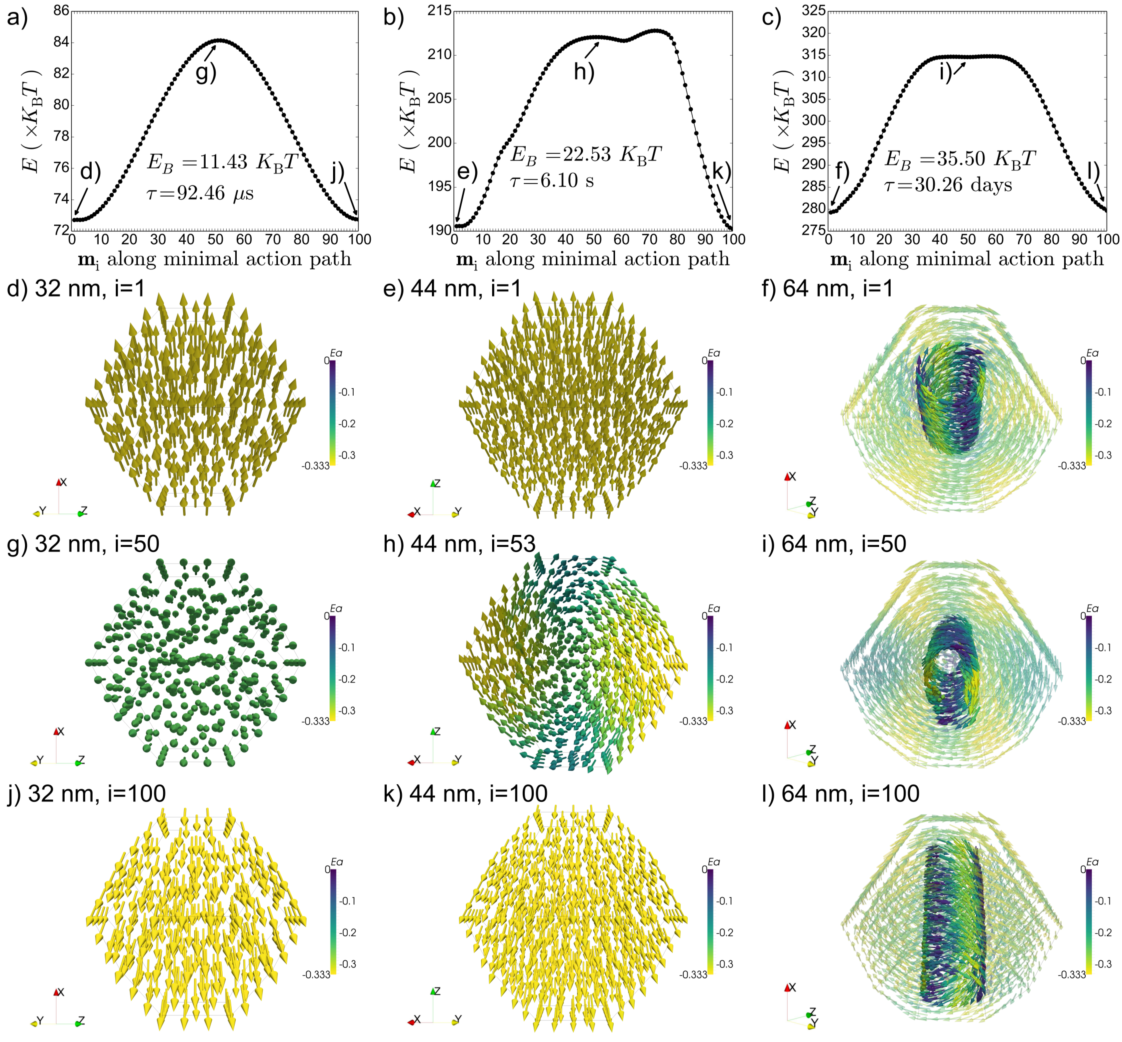
\includegraphics[width=\textwidth]{Figure_07_HR.pdf}
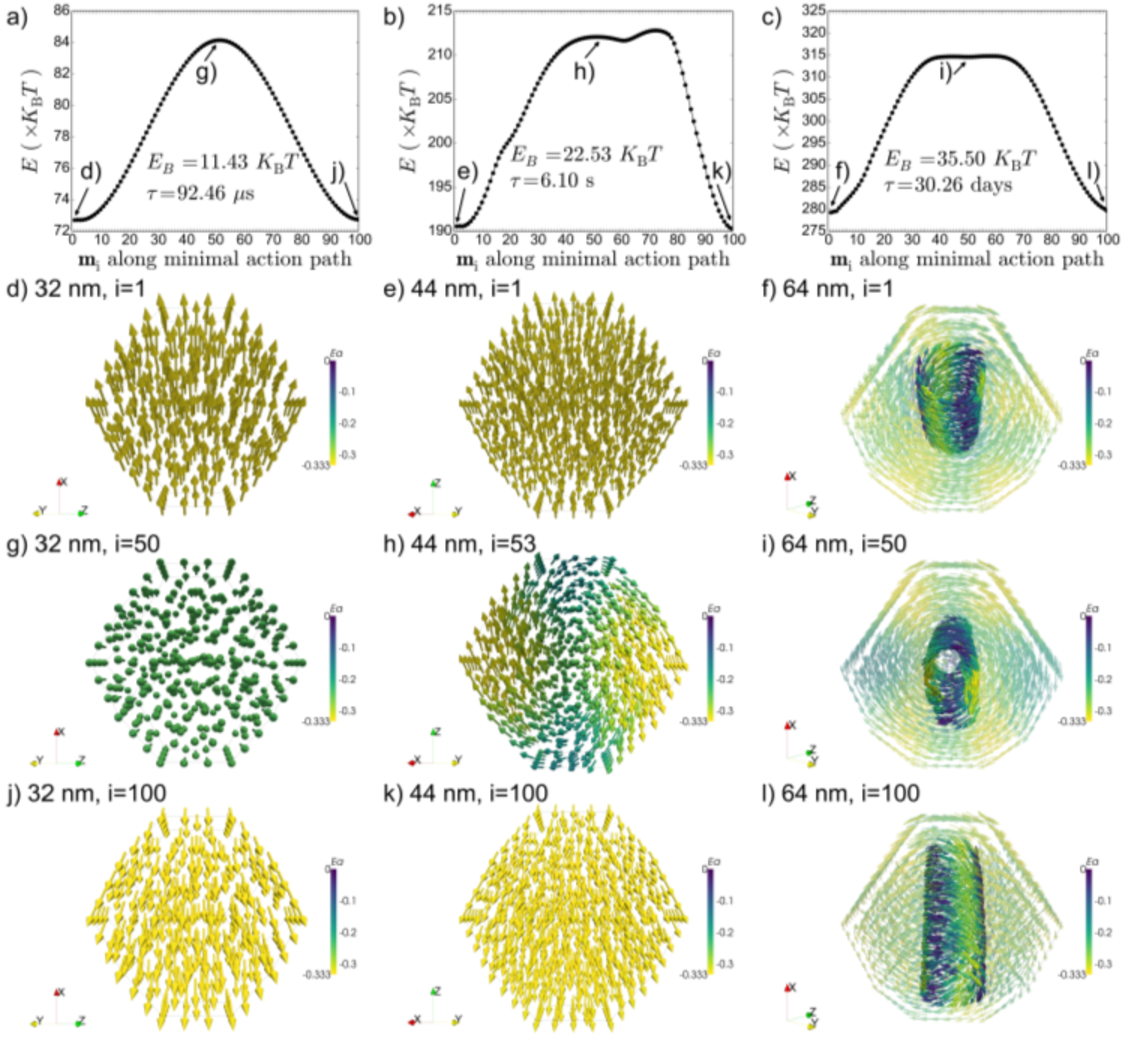
\includegraphics[width=\textwidth]{research-1/figs/Figure_07.pdf}
\caption[Typical action-minimising paths]{Typical action-minimising paths. The regular truncated octahedra illustrate the typical AMPs found for all the (truncated) octahedral shapes. Well below the SD--PSD threshold the AMP between SD configurations is a coherent rotation (left column). The energy along the AMP is a single bump (a) and the energy barrier is an intermediate-aligned SD state (d). At sizes just below the SD--PSD threshold the AMP is still between SD states, but via a curling mode (vortex nucleation) (center column). Starting from SD (e), a vortex is nucleated (h) then unwinds to an intermediate-aligned SD state which has the highest energy along the AMP (not shown). Then, the final SD state (k) is reached via coherent rotation. This makes the energy along the AMP more complex and asymmetric (b). Well above the SD--PSD threshold, once the EAV has the lowest energy, the AMP is via a structured rotation of the vortex core (right column). The transition is between two EAVs with the same chirality (f, l) as a change of chirality produces prohibitively large energy barriers. In the AMP there is an IAV sitting in its own shallow LEM (i). The energy barrier is the one that separates the EAVs from the IAV. However, as the grain grows, the IAV LEM becomes more shallow and the energy along the AMP flattens (c). Colour represents the MCA energy normalised by $|K_1|$. The energies along the AMPs are plotted in units of $K_\text{B}T$, with $T=300\,\text{K}$. The left column of Video 1 (supplementary material) shows these transitions.}
\label{fig7}
\end{figure}

\subsubsection{Cuboctahedra}
The cuboctahedra show a very different behaviour. Their relaxation times increase exponentially for the SD to SD transitions, but do not drop for the first PSD to PSD transitions, at 48$\nm$, which are hard-aligned to hard-aligned (Fig. \ref{fig8}, left column) and pass through a dIAV (Fig. \ref{fig8}g). The energy barrier is an IAV (Fig. \ref{fig8}j). The relaxation times for these transitions then decrease as the HAV and dIAV energies get closer until, at 66$\nm$, the GEM is a dIAV. Then, since the straight IAV has a very high energy, transitions in which the dIAV ends reattach to contiguous faces are unfavorable. The transition with the lowest energy barrier is between two distorted vortices like the ones shown in Figs. \ref{fig8}e, k, which are (though distorted) [0$\bar{1}\bar{1}$]- and [1$\bar{1}$0]-aligned. The transition preserves the shape of the distorted vortex as it structuredly rotates keeping its ends attached to the square faces.\par

The relaxation times for this type of transitions plateau at a few microseconds up to 74$\nm$. In Fig. \ref{fig3}j the energies of the dIAV and the EAV intersect at roughly 90$\nm$ and are very close up to 120$\nm$. Since the transition between two EAVs is likely to go through a dIAV, it is not expected that the relaxation time for EAV to EAV transitions will rapidly increase until sizes much larger than 90$\nm$. Indeed, we find that only for the particles larger than 110$\,$nm the relaxation times start to grow exponentially{\textemdash}though at a rate slower than for (truncated) octahedra transitions{\textemdash}surpassing 4 billion years at roughly 134$\nm$ (Fig. \ref{fig9}c). A typical transition of this type at 132$\nm$ is shown on the right column of Fig. \ref{fig8} between [111]- and [11$\bar{1}$]-aligned vortices via vortex distortion (not shown). The highest energy state along the path is a straight IAV (Fig. \ref{fig8}i). The right column of Video 1 (supplementary material) shows these transitions.
\begin{figure}
\centering
%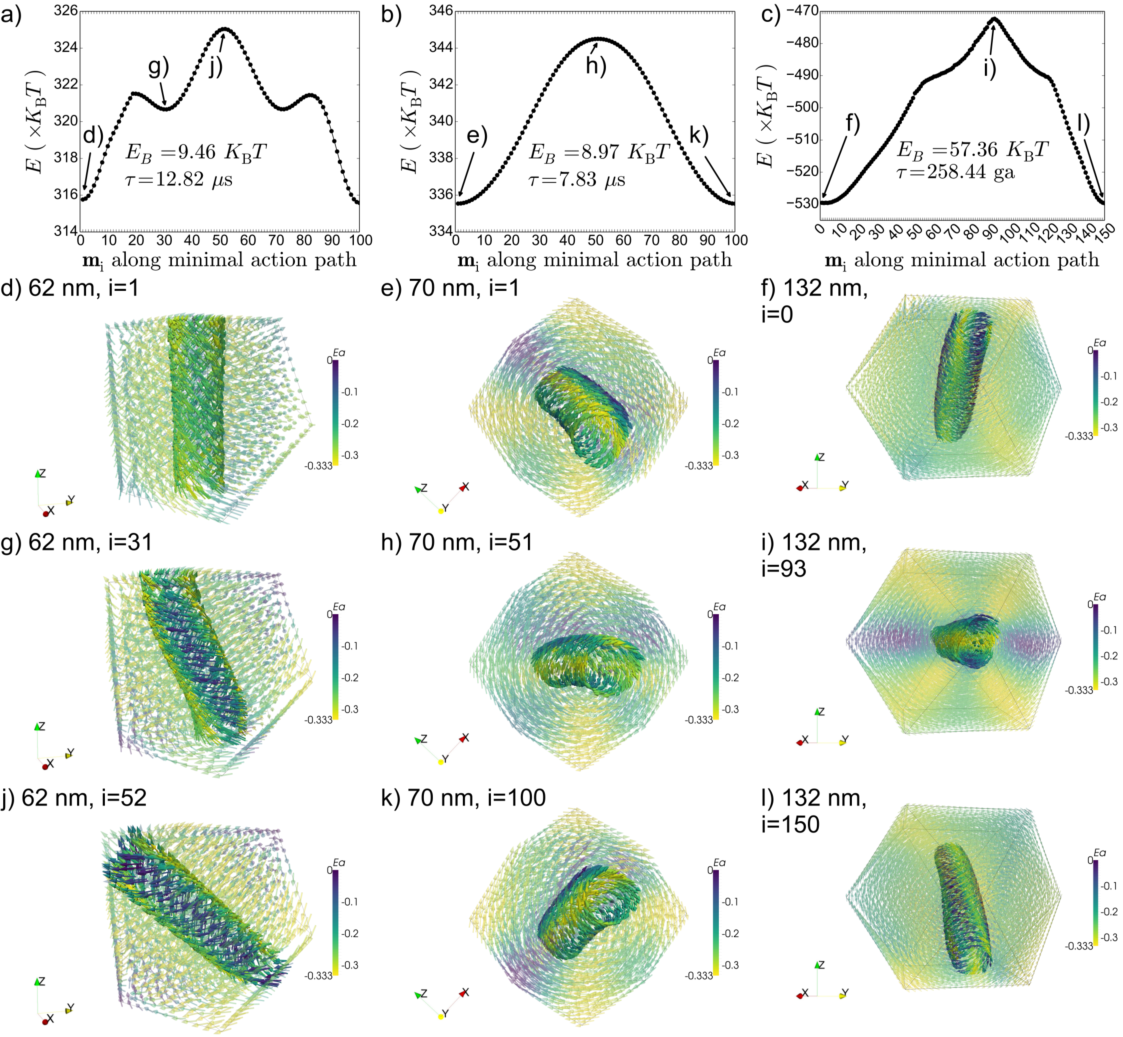
\includegraphics[width=\textwidth]{Figure_08_HR.pdf}
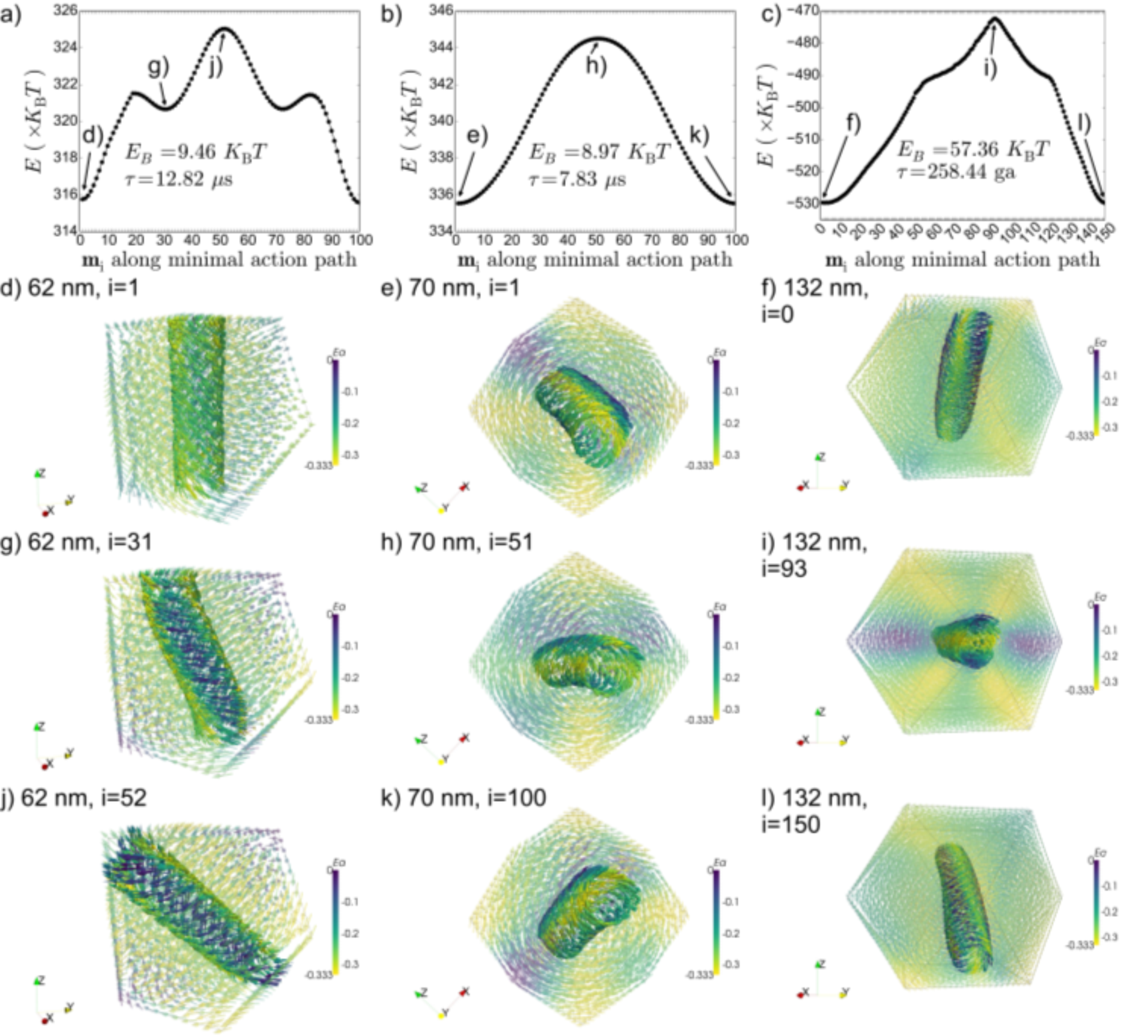
\includegraphics[width=\textwidth]{research-1/figs/Figure_08.pdf}
\caption[Action-minimising paths for the cuboctahedra]{Action-minimising paths for the cuboctahedra. The cuboctahedra showed different AMPs above the SD--PSD threshold from the rest of the shapes. Above the SD--PSD threshold, and up to 66$\nm$, the lowest energy state for the cuboctahedron is a HAV. Transitions between HAVs (left column) occur via a distortion (g) and structured rotation (j) of the vortex core. The energy barrier is an IAV (j). The dIAV along the AMP (g) sits in its own LEM, forming a three-bump energy barrier (a). The dIAV becomes the lowest energy from 66$\nm$. Transitions between dIAVs (center column) form a single bump energy barrier (b). The transition is a structured rotation of the distorted vortex, keeping attached to the same surface (e, h, k). Once the lowest energy is an EAV, transitions between these (right column) occur via a distortion and structured rotation of the vortex core. The energy barrier is an IAV (i). Colour represents the MCA energy normalised by $|K_1|$. The energies along the AMPs are plotted in units of $K_\text{B}T$, with $T=300\,\text{K}$. The right column of Video 1 (supplementary material) shows these transitions.}
\label{fig8}
\end{figure}

\subsubsection{Discussion}
Fig. \ref{fig9} summarizes the results of the relaxation times obtained for the five (truncated) octahedral shapes in the 30$\nm$ to 74$\nm$ range and the relaxation times for the cuboctahedra in the 120$\nm$ to 134$\nm$ range (Fig. \ref{fig9}, inset). For all shapes, except the cuboctahedral, the general behaviour is an exponential increase of the relaxation times for the SD to SD transitions from a few tens of microseconds to a few seconds for the regular truncated octahedra and up to 12 days for the octahedra, followed by a sharp drop at 46$\nm$ (for the regular truncated octahedra) to 50$\nm$ (for the octahedra). This drop in the relaxation times marks the SD--PSD threshold. Then, the PSD to PSD transitions have increasingly lower relaxation times until reaching a global minimum at $\roughly$50$\nm$ to $\roughly$54$\nm$. Once the GEM is the EAV the relaxation time shoots up exponentially with crystal growth, surpassing 4 billion years at $\roughly$68$\nm$ to $\roughly$72$\nm$.
\begin{figure}
\centering
%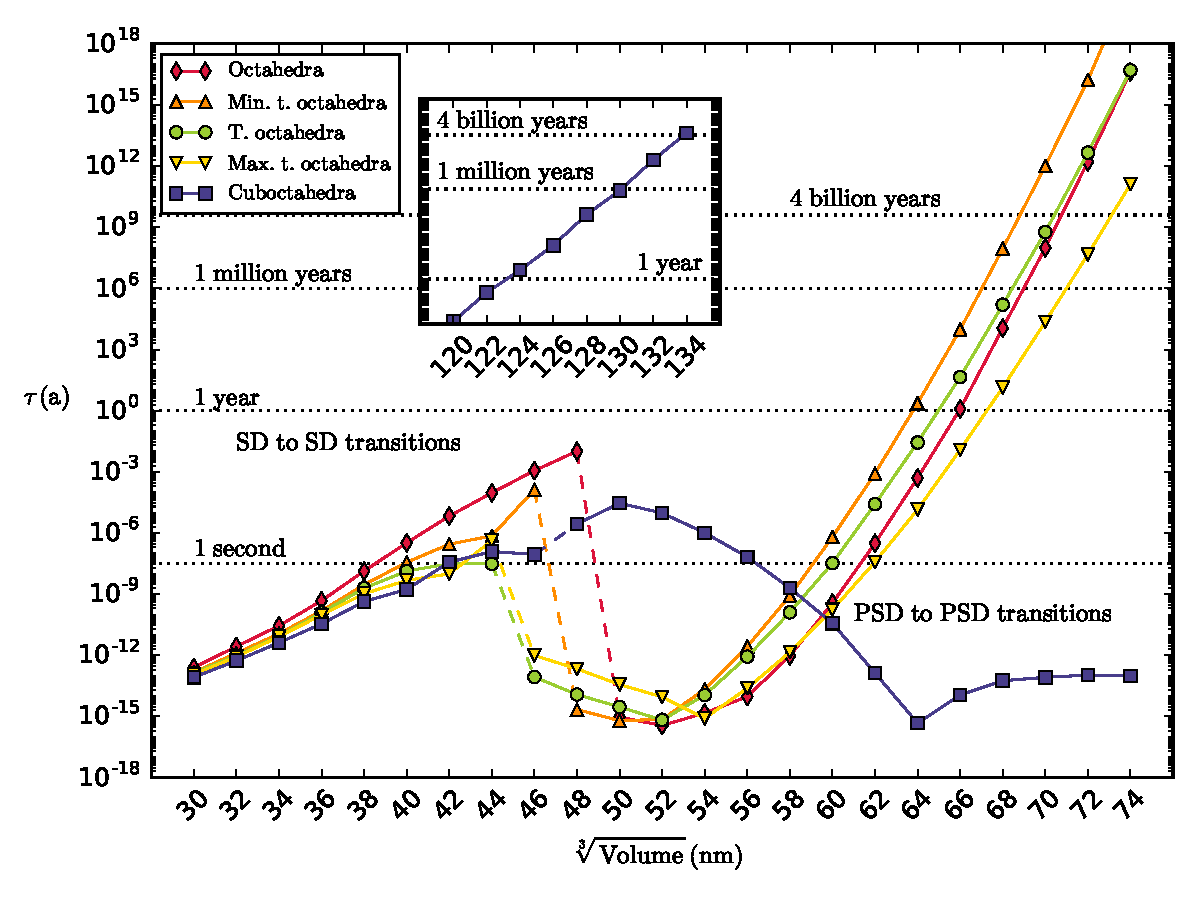
\includegraphics[width=\textwidth]{Figure_09_HR.pdf}
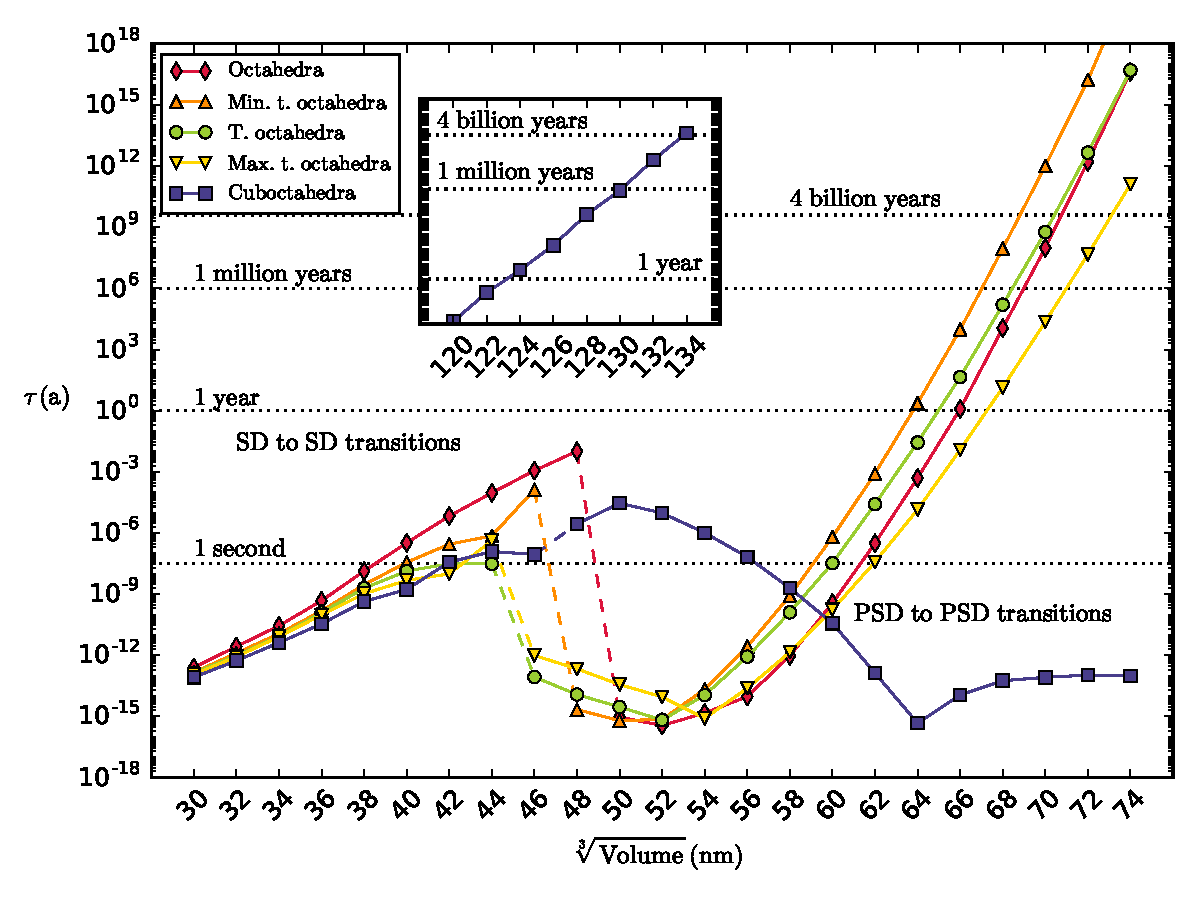
\includegraphics[width=\textwidth]{research-1/figs/Figure_09.pdf}
\caption[Relaxation times for the euhedral shapes]{Relaxation times for the euhedral shapes. The relaxation times are calculated with $\tau_0=1\,\text{ns}$, $T=300\,\text{K}$. $\tau$ increases exponentially for the SD--SD transitions, but reaches only laboratory scale stabilities before the SD--PSD threshold. The (truncated) octahedral shapes show a dip in the stability in the lower end of the PSD range for HAV--HAV and IAV--IAV transitions, reaching a minimum at $\roughly$52$\nm$. Once the EAVs have the lowest energies, the relaxation times grow exponentially with size, reaching four billion years from $\roughly$70$\nm$. The cuboctahedra, however, show a different behaviour: they do not show a dip in the stability for the first HAV--HAV transitions, but with increasing size they produce lower relaxation times as the energy of the dIAV gets closer. The relaxation times for the transitions between dIAVs plateau up to 74$\nm$. Exponential growth of the relaxation times occurs from $\roughly$110$\nm$ (inset), surpassing four billion years from $\roughly$134$\nm$.}
\label{fig9}
\end{figure}

These calculations show that equant, non-interacting, room-temperature SD grains of greigite are on a geological timescale, SP given that the largest relaxation time found for SD particles (octahedra) of 12 days is only stable on laboratory timescales. Therefore, the expected SP--SSD threshold does not exist but rather a SP--PSD threshold since it is only the PSD grains which can hold a remanence for extended periods of time. \citet{Muxworthy2013} estimated the energy barriers for non-interacting cubes of greigite from the anisotropy energy surface and found a SP--SSD threshold of 56$\nm$, for a relaxation time of four billion years. In this study the blocking volumes for cubes and spheres were not calculated as these are not naturally occurring morphologies for greigite. However, given the results for the five (truncated) octahedral shapes, it is unlikely that a SP--SSD threshold should exist for either cubes or spheres.\par

Since the relaxation times for the larger SD particles are so small and since the transitions from SD to SD just before the GEM becomes PSD are through a curling mode (vortex nucleation), we conclude that the SD--PSD threshold is defined only by the first intersection of a PSD energy curve with the SD energy curve, $d_0$ (Figs. \ref{fig2}b, \ref{fig3}b, d, f, h, j, l). That SD--SD transitions just below the SD--PSD threshold occur via a curling mode was also observed for magnetite by \citet{Enkin1994} and shows that greigite particles are likely to show PSD aspects even below the SD--PSD threshold. It is highly unlikely that metastable SD grains exist beyond $d_0$ in the absence of grain--grain interactions. The relaxation times between PSD states just above $d_0$ are the shortest of all and only start to grow exponentially for the EAV to EAV transitions. We thus conclude that the PSD--MD transition through a crystal growth mechanism, must occur through an EAV path.\par

The splitting of the energy curves' intersections exhibited by the cuboctahedra not only has repercusions on the SD--PSD threshold, but also on its stability against thermal fluctuations. All the (truncated) octahedral particles have blocking volumes of $\roughly$72$\nm$ while for the cuboctahedra this volume is $\roughly$134$\nm$. This could be explained by the fact that the first PSD to PSD transitions, between hard-aligned PSD states, traverse through IAVs (Fig. \ref{fig8}, left column): as the cuboctahedral particle grows, the energy difference between the IAV and HAV becomes smaller (Fig. \ref{fig3}j) and this is reflected in a diminishing of the relaxation times for this type of transition (Fig. \ref{fig9}). Since for the rest of the shapes the PSD and SD energy curves all meet in a relatively short span, this effect of diminished stability with increasing size only lasts for a much smaller range of sizes, and once the EAV is the GEM, the relaxation times for transitions between this type of domain state grow very rapidly. However, for the cuboctahedra the EAV becomes the GEM at a larger size than for the rest of the shapes and the energy difference with the dIAV, through which the AMP goes through, is very small.\par
%-----------------------------------------------------

\section{Conclusion}
We have presented calculations of the SD--PSD threshold for realistic shapes of equant greigite grains. We have found that octahedral shapes have the largest SD--PSD threshold $d_0\approx56\,\text{nm}$, a value lower than the threshold obtained for magnetite octahedra by \citet{Witt2005} of $\roughly$73$\nm$. This value decreases by the effects of truncation to $d_0\approx53\,\text{nm}$ for the regular truncated octahedra and further down to $d_0\approx50\,\text{nm}$ for the cuboctahedra. The SD--PSD threshold for greigite cubes was lower ($d_0\approx 52\,\text{nm}$) than that of \citet{Muxworthy2013} (=58$\nm$); however, we used a different value for $M_\text{S}$. When we modelled using the same parameters as \citet{Muxworthy2013} we found excellent agreement, obtaining a $d_0\approx 60\,\text{nm}$.\par
NEB method calculations of the room-temperature blocking volumes of greigite show the importance of thermal fluctuations in determining the magnetic structure of a ferromagnetic grain beyond simpler micromagnetic models. We found that equant SD greigite grains cannot be expected to be reliable palaeomagnetic recorders: only PSD grains larger than $\roughly$72$\nm$ are able to hold a remanence in geological timescales, though there is a strong grain shape dependence.\par

We found that cuboctahedral particles have a blocking volume of $\roughly$134$\nm$, a volume almost seven times larger than for the (truncated) octahedral particles. This highlights the importance of addressing not only the size distribution in sedimentary rock samples, but also the shapes of the greigite grains present.\par
We found that the transitions between PSD states occur via well-defined states by a structured rotation of the vortex cores. This could be useful for future analytical models beyond the SD coherent rotation theory.\par

Although in this study we have disregarded the effects of particle elongations, which are sure to effect the blocking volumes \citep{Muxworthy2013}, our results are representative of widespread authigenic greigite grains of abiotic origin. The effects of grain--grain magnetostatic interactions have also been excluded from this study. Isolated greigite grains are not very common, rather, natural samples show that greigite is more commonly aggregated in tight clusters. However, this study provides a stepping-stone towards understanding the more complex greigite clusters.\par

%-----------------------------------------------------
\renewcommand\bibname{{References}}
\bibliographystyle{elsarticle-harv}
\bibliography{references}
%-----------------------------------------------------

%\chapter{First-order reversal curve (FORC) diagrams of nanomagnets with cubic magnetocrystalline anisotropy}
\label{ch:res-2}
\fancyhead[L]{Chapter 3. Single-domain FORC diagrams}
\fancyhead[C]{}
\fancyhead[R]{}
\fancyfoot[C]{\thepage}

This Chapter is submitted for publication as Valdez-Grijalva, M. A., Muxworthy, A. R., 2018. First-order reversal curve (FORC) diagrams of nanomagnets with cubic magnetocrystalline Anisotropy. J. Magn. Magn. Mater., in review.

\section*{Abstract}
First-order reversal curve (FORC) diagrams are increasingly used as a material's magnetic domain state fingerprint. FORC diagrams of noninteracting dispersions of single-domain (SD) particles with uniaxial magnetocrystalline anisotropy (MCA) are well studied. However, a large class of materials possess a cubic MCA, for which the FORC diagram properties of noninteracting SD particle dispersions are less understood. A coherent rotation model was implemented to study the FORC diagram properties of noninteracting ensembles of SD greigite (Fe$_3$S$_4$), and iron (Fe). FORC diagrams contain mixed information of irreversible and reversible rotations of the magnetisations. The pattern formation mechanism is identified and related to the irreversible events the individual particles undergo. The purely reversible signal is determined based on the FORC diagram properties of the individual particles. Our results support the utility of FORC diagrams for the identification of noninteracting to weakly-interacting SD particles with cubic MCA.\par

%%%%%%%%%%%%%%%%%%%%%%%%%%%%%%%%%%%%%%%%%%%%%%%%%%%%%%%%%%%%

\section{Introduction}
Ferromagnetic materials exhibit magnetic hysteresis: the dependence of the material's magnetisation $\boldsymbol{M}$ on its magnetic history \citep{Mayergoyz1986}. The hysteretic response of a material is obtained by a series of measurements of its scalar magnetisation $M=\boldsymbol{M} \cdot \boldsymbol{\hat{n}}$ as a function of the applied magnetic field $\boldsymbol{H}=H\boldsymbol{\hat{n}}$. To trace a hysteresis loop the magnetic field strength $H$ is slowly decreased from its saturation value $H=H_{\text{sat}}$ down to $H=-H_{\text{sat}}$, followed by the slow increase up to $H=H_{\text{sat}}$.\par

First-order reversal curves (FORCs) are a set of partial hysteresis loops, each starting at a saturation field $H=H_{\text{sat}}$, followed by the quasi-static decrease of the applied field strength down to $H=H_a$. From $H_a$, the field strength is increased back to $H=H_{\text{sat}}$ to trace a given curve labelled by its $H_a$ value. On each FORC, the scalar magnetisation is then a function $M=M(H_b, H_a)$ of the applied field $H=H_b$ and the $H_a$ value of the given curve ($H_a \leq H_b$).\par
The FORC distribution, an empirical analog of the Preisach weight function based on the experimental protocol described above, is defined as the second order mixed partial derivative \citep{Roberts2000}
\begin{equation}\label{forc}
\rho = \rho(H_b, H_a) = -\frac{1}{2}\frac{\partial^2 M}{\partial H_a \partial H_b},
\end{equation}
which must be understood in some weak sense to allow the discontinuous $M$. Contour plots of the FORC distribution (Eqn. \ref{forc}) are known as FORC diagrams and have been increasingly used by the wide magnetics community as a proxy for the magnetic domain state and switching behaviour of a variety of magnetic systems \citep{Pike1999,Pike2005,Roberts2000,Biasi2016,Proenca2017}.\par

Based on Stoner-Wohlfarth theory \citep{Stoner1948} significant progress has been made towards understanding the contribution of fine magnetic single-domain (SD) particles with uniaxial magnetocrystalline anisotropy (MCA) to the FORC diagram properties of interacting and noninteracting dispersions \citep{Newell2005,Egli2010,Biasi2016}. However, many materials including the most abundant ferromagnetic minerals on Earth possess a cubic MCA.\par

The general hysteretic properties of noninteracting dispersions of particles with cubic MCA has been previously studied \citep{Usov1997,Walker1993}. The cubic MCA system is more complicated than the uniaxial due to the existence of more local energy minima (LEM) and the mechanism behind the FORC diagram pattern formation is not yet as well understood as the uniaxial case.\par

Previous studies of FORC diagram pattern formation by minerals with cubic MCA used micromagnetics \citep{Muxworthy2004} and dipole-dipole modelling \citep{Harrison2014} to study the influence of magnetostatic interactions on the FORC diagram. However, the fully noninteracting case remains unknown as these studies rely on specific arrangements of particles positions and orientations, thus by definition cannot completely isolate the purely noninteracting contribution.\par

In this study we present an approach for numerically calculating the FORC diagram of a uniform noninteracting dispersion of SD particles with cubic MCA. The magnetic parameters of: greigite (Fe$_3$S$_4$), saturation magnetisation $M_s=2.7\times 10^5 \, \text{A/m}$ \citep{Li2014} and first anisotropy constant $K_1=-1.7\times 10^4 \, \text{J/m}^3$ \citep{Winklhofer2014}; and metallic iron (Fe), $M_s=1.7\times 10^6 \, \text{A/m}$ \citep{Dunlop} and $K_1=4.8\times 10^4 \, \text{J/m}^3$ \citep{Graham1958} have been used due to their opposing $K_1$ signs, their relatively high anisotropy and their importance for technological applications as well as the Earth sciences.\par

\section{Method}
\subsection{The FORC model}
In an ensemble of identical, randomly aligned particles the probability of a given particle orientation is uniform over the sphere. If the ensemble is noninteracting (dilute) then the ensemble has a magnetic response
\begin{align}
M &= M(H_b, H_a) \nonumber \\
  &= {\int^{2\pi}_{0}}{\int^{2\pi}_{0}} m'(H_b, H_a, \theta, \phi)\,\,\sin\theta\,\text{d}\theta\,\text{d}\phi,
\end{align}
where $m'(H_b, H_a, \theta, \phi)$ is the magnetisation of a particle at $(H_b, H_a)$ when the applied field is directed along the unit vector $\boldsymbol{\hat{n}} = \boldsymbol{\hat{e}}_r + \theta\boldsymbol{\hat{e}}_\theta + \phi\boldsymbol{\hat{e}}_\phi$. Given the symmetry of the cubic anisotropy system, the integration can instead be carried out over the subdomain $\mathbf{I} \equiv [0, \pi/2] \times [0, \pi/2]$, so:
\begin{align}\label{integral}
M^{\dagger} &= M^{\dagger}(H_b, H_a) = \frac{M(H_b, H_a)}{8} \nonumber \\
            &= {\int^{\pi/2}_{0}}{\int^{\pi/2}_{0}} m'(H_b, H_a, \theta, \phi)\,\,\sin\theta\,\text{d}\theta\,\text{d}\phi.
\end{align}
\par

We calculate Eqn. (\ref{integral}) using the backtracking line-search gradient method outlined in Section \ref{grad method} to obtain each $m'(H_b, H_a, \theta, \phi)$ over a uniform grid $G \equiv \{i\pi/100: i=0,\ldots,50 \} \times \{j\pi/100: j=0,\ldots,50 \}$ with the evaluation performed in the center of the cells:
\begin{align}
M^{*} &= M^{*}(H_b, H_a) \nonumber \\
      &= {\sum_{i}}{\sum_{j}} m'(H_b, H_a, \theta_i, \phi_j)\,\,\sin\theta_i\,\Delta\theta\,\Delta\phi.
\end{align}
\par

The hysteresis loop of a single particle in the simplest case is a hysteron with switching fields $H^{-}$ and $H^{+}$. In such a case, all the FORCs are contained in the main branches of the hysteresis loop (i.e., the field-descending and -ascending curves). The FORC distribution (Eqn. (\ref{forc})) is, accordingly:
\begin{equation}\label{forc hysteron}
\rho = -\frac{1}{2} \delta \left( H_a - H^{-} \right) \left\{ \left[ \frac{\text{d} m' }{\text{d}H_b} \right] + \left[ m' \right] \delta(H_b - H^{+}) \right\},
\end{equation}
where $\left[ m' \right]$ is, up to its sign, the size of the magnetisation discontinuity at the switching field $H^{+}$ and $\left[ \text{d} m' / \text{d}H_b \right]$ the difference in the slopes between the main branches. The distribution has two parts: tail and front. The front contains the information about the magnetisation behaviour at the switching fields and has a delta-like support. The tail has support along a line $(H_a=H^{-}, H_b<H^{+})$ and contains information about the slopes traced by the reversible motions. This contribution is usually an order of magnitude lower than the front so the reversible information is mostly obscured in a FORC diagram. We can, however, identify where the fronts are (from the switching fields) and remove them from the FORC distribution to obtain purely reversible FORC distributions.\par

For a single particle, the computation of the complete set of FORCs can be simplified if we note that each curve consists mostly of reversible motion with only a few irreversible jumps at the switching fields. This means that all the FORCs with $H_a$ larger than the first switching field are implicitly calculated in the main branch of the hysteresis loop. Similarly for all the $m'(H_b, H_a)$ between the first (second) and second (third) switching field, if there are more than one (two) irreversible jumps, and the $m'(B_b, B_a)$ between the last switching field and $-H_{\text{sat}}$ . All that is left then, after calculating the hysteresis main branch, is to calculate the FORCs starting at $H_a$ values corresponding to the switching fields (Fig. \ref{FIG_E01}(b)). Once obtained, all $m'(H_b, H_a)$ form a grid $m_i^j$ on which the FORC distribution can now be calculated (Fig. \ref{FIG_E01}(c)). The calculation is done at each grid point by least-square fitting a second degree polynomial surface on a subgrid $\left\{ m_{i+k}^{j+l}:\, k, l=-\text{SF},\cdots,\text{SF} \right\}$, where SF is the so-called smoothing factor, taking care to exclude points with $H_b<H_a$; from the general equation of the fitted polynomial surface $a_0 + a_1 H_a + a_2 H_b + a_3 H_a H_b + a_4 H_a^2 + a_5 H_b^2 = 0$ the FORC distribution is simply $-a_3/2$ \citep{Pike1999}.
\begin{figure}
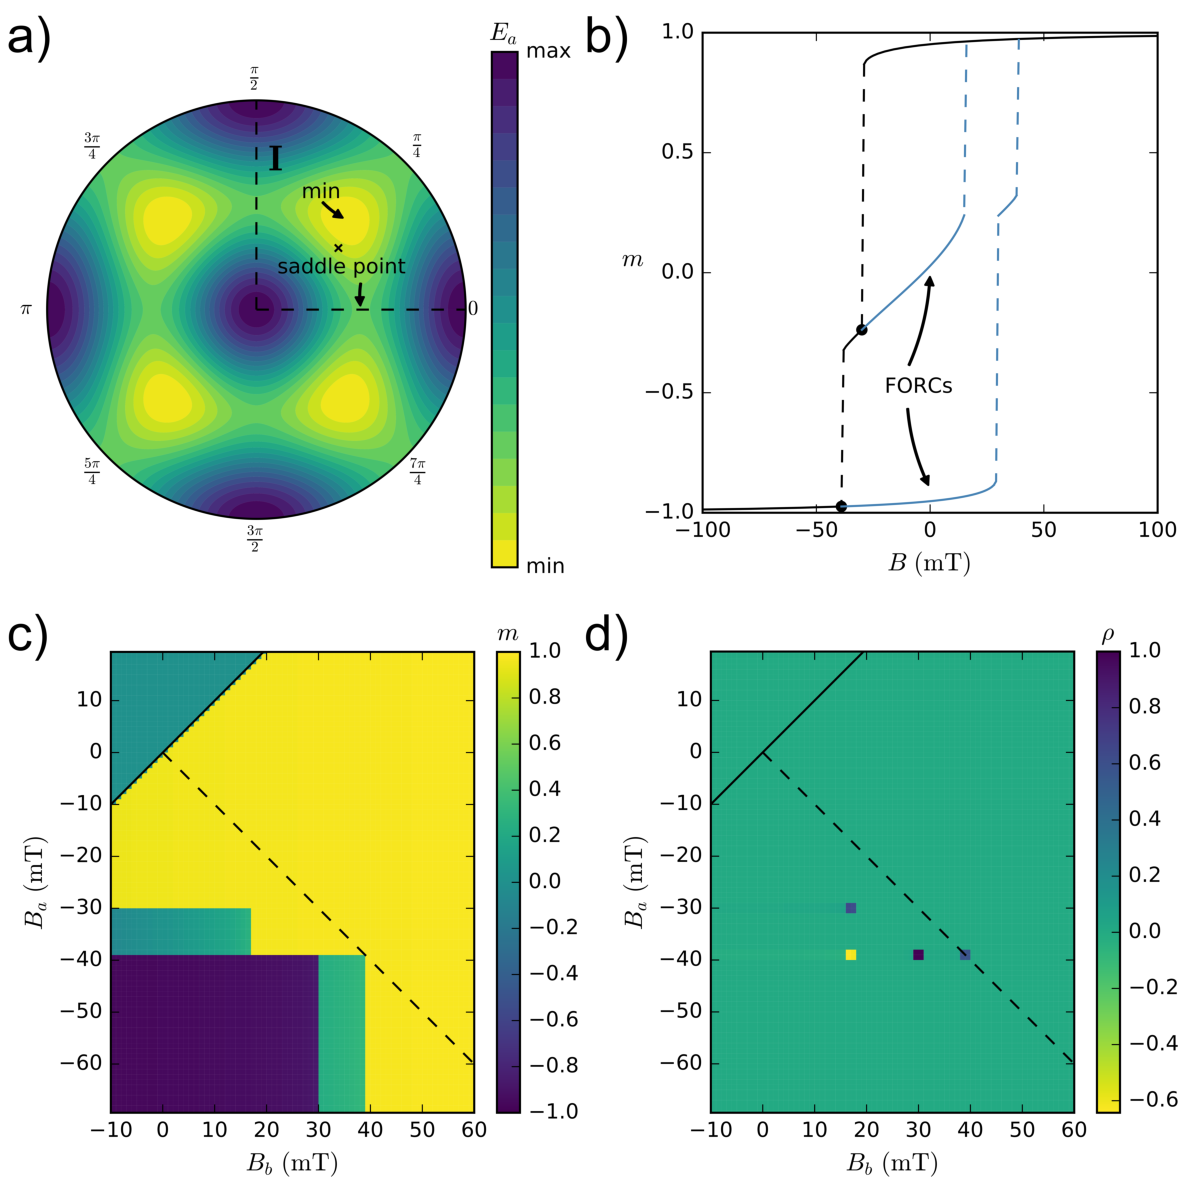
\includegraphics[width=\textwidth]{research-2/figs/FIG01.pdf}
\caption[Basic FORC modelling concepts]{Basic concepts. a) Energy landscape projection in polar coordinates for $K_1<0,\, K_2=0$; b) a complete set of FORCs for $\theta ,\,\phi$ as marked by the $\boldsymbol{\times}$ in a); c) the reduced magnetisation $m(B_b=\mu_0 H_b, B_a=\mu_0 H_a)$; d) the corresponding FORC distribution (normalised) with SF=1. The FORC distribution fronts and tails coincide with the sharp edges of $m(B_b, B_a)$.}
\label{FIG_E01}
\end{figure}
\par
A SF=1 was used to calculate the FORC distribution of each individual particle to limit the smoothing and retain the delta-like profile of the FORC distribution as much as possible (Figure \ref{FIG_E01}(d).) In this manner, FORC distributions were obtained by adding those of each individual particle instead of calculating $\rho$ on the ensemble magnetic response; essentially, this is what allows to remove the irreversible contribution from the FORC distribution of each particle and obtain the purely reversible FORC signal. FORC diagrams with SF=4 were also calculated; in these the reversible and irreversible contributions are mixed. Using a nonlinear scale, however, it is possible to discern the low-valued reversible contributions.\par

\subsection{Backtracking line-search gradient-descent method}\label{grad method}
A small spherical ferromagnetic particle in the single-domain (SD) state is modelled as a magnetic dipole with constant magnitude $|\boldsymbol{M}| = M_s$, the saturation magnetisation of the material. The magnetic Gibbs free-energy density of the particle is then the sum of the magnetocrystalline anisotropy (MCA) and the external field energy densities:
\begin{equation}\label{EQ:ENERGY}
E = E_a +E_z
\end{equation}
with
\begin{align}
E_a &= \frac{K_1}{2}\sum_{i\neq j}\alpha_i^2 \alpha_j^2 + K_2 \prod_i \alpha_i^2,\\
E_z &= - M_s\left( \boldsymbol{m} \cdot \boldsymbol{B}\right) = -M_sB \left( \alpha\chi + \beta\psi + \gamma\omega\right);
\end{align}
where $\alpha_i = \left(\alpha,\,\beta,\,\gamma\right)$ are the direction cosines of the reduced magnetisation $\boldsymbol{m} = \boldsymbol{M}/|\boldsymbol{M}|$ and $\left(\chi,\,\psi,\,\omega\right)$ those of the external field $\boldsymbol{B}=\mu_0 \boldsymbol{H}$; $K_1$ and $K_2$ the first and second MCA constants. From thermodynamics it is known that a system is spontaneously driven towards states with locally minimal Gibbs free-energy. Therefore, we are concerned with finding the LEM of the function $E=E(\boldsymbol{m},\,\boldsymbol{B})$.\par

Since the reduced magnetisation vector is unitary, it is natural to express the energy in the spherical coordinate system $E=E(\boldsymbol{m}=\boldsymbol{m}(\theta,\,\phi),\, \boldsymbol{B})$ ($\theta, \phi$ the polar and azimuthal angles, respectively):
\begin{align}
E_a &= K_1 \sin^2\theta\left[ \cos^2\theta + \left( \sin\theta\cos\phi\sin\phi\right)^2 \right] \nonumber \\
    &+ K_2\sin^2\theta \left( \sin\theta\cos\theta\sin\phi\cos\phi \right)^2, \label{EQ:ENERGY anis} \\
E_z &= -M_sB \left( \chi\sin\theta\cos\phi + \psi\sin\theta\sin\phi + \omega\cos\theta\right). \label{EQ:ENERGY ext}
\end{align}
$E_a$ minima and maxima lie along crystallographic orientations depending on the sign of $K_1,\,\,K_2$ and the ratio $|K_2| / |K_1|$. For $K_1<0$ ($K_2=0$) the easy axes (minima) are the $<$111$>$ and the hard (maxima) the $<$100$>$; the $<$110$>$ are saddle points (Fig. \ref{FIG_E01}(a)). When $K_1>0$ ($K_2=0$) instead, the easy axes become the $<$100$>$ and the hard the $<$111$>$ while the $<$110$>$ remain as saddle points.\par

From eq. (\ref{EQ:ENERGY}), (\ref{EQ:ENERGY anis}--\ref{EQ:ENERGY ext}), the gradient is then
\begin{align}
  \nabla E &= \hat{e}_\theta \left( E_a + E_z \right)_\theta + \hat{e}_\phi \left( E_a + E_z \right)_\phi  \nonumber \\
           &= \hat{e}_\theta \left( (E_a)_\theta + (E_z)_\theta \right) + \hat{e}_\phi \left( (E_a)_\phi + (E_z)_\phi \right);
\end{align}
where
\begin{align}
( E_a )_\theta &= 2\sin\theta\cos\theta\left\{ K_1  \left[ 2\left( \sin\theta\sin\phi\cos\phi \right)^2 \right. \right. \nonumber \\
             &- \left. \sin^2 \theta + \cos^2 \theta \right] \nonumber \\
             &+ \left. K_2 \left[ 2( \sin\theta\cos\theta\sin\phi\cos\phi )^2 - \sin^4\theta \right] \right\}, \\
( E_z )_\theta &= - M_s B ( \chi\cos\theta\cos\phi + \psi\cos\theta\sin\phi - \omega\sin\theta ) \\
( E_a )_\phi &= 2\sin^4\theta\sin\phi\cos\phi \left( K_1+K_2\cos^2\theta\right) \nonumber \\
            &\times \left( - \sin^2\phi + \cos^2\phi \right) \\
( E_z )_\phi &= -M_s B\sin\theta \left( - \chi\sin\phi + \psi\cos\phi \right).
\end{align}
\par
A backtracking line-search gradient-descent method \citep{Armijo1966} was implemented to simulate hysteresis loops and first-order reversal curves of nanomagnets with cubic MCA. The Armijo-Goldstein control parameters $c=1\times10^-4$, $\tau=1/2$ were used in this study. These ensure that the minimiser follows the gradient-descent direction very closely (Fig. \ref{FIG_E02}). An example of the code can be consulted in Appendix A.
\begin{figure}
\includegraphics[width=\textwidth]{research-2/figs/FIG02.pdf}
\caption[The behaviour of the minimiser during irreversible motion]{The behaviour of the minimiser during irreversible motion along the main branch of the FORCs shown in Fig. \ref{FIG_E01}(b). a) When the field is -30$\,$mT the magnetisation irreversibly rotates from its position in the positive octant ($x,y,z>0$) (grey dot) to the one with $z<0$, where a local energy minimum is found (black dot). As the field strength is further increased the local energy minimum becomes more shallow until b) at -39$\,$mT an energy gradient causes the irreversible motion to the negative octant ($x,y,z<0$) where saturation occurs.}
\label{FIG_E02}
\end{figure}
\par

\section{Results and Discussion}
The calculated FORCs for a given field orientation are shown in Fig. \ref{FIG_E01}(b). Fig. \ref{FIG_E01}(c--d) shows the magnetisation as a function of $(B_b, B_a)$ and the corresponding FORC diagram (normalised). It is seen that the distribution is a collection of tail/front pairs like Eqn. \ref{forc hysteron} along the discontinuities in $m(B_b, B_a)$. A negative delta-like source at $(B_b=17\,\mathrm{mT},\,B_a=-39\,\mathrm{mT})$ is caused by the curve with $B_a=-38\,$mT going back to positive saturation at $B_b=17\,$mT while the one with $B_a=-39\,$mT remains in its negative saturation state up to $B_b=30\,$mT. These type of strong, highly-localised FORC distribution negative sources are then due to irreversible events on different FORCs. These strong, negative delta-like sources cannot occur in uniaxial particles which have only one irreversible event along the hysteresis main branch; low-valued negative delta-like sources are possible in uniaxial systems for the particles with easy axis almost normal to the applied field which experience very small irreversible upward jumps \citep{Stoner1948,Newell2005}.\par

The particles that have an easy axis alignment closer to the external field produce highly-symmetric, hysteron-like hysteresis curves which are responsible for the accumulation of positive delta-like sources along the central ridge (the line $H_a=-H_b$). The material with the highest coercivities $B_\text{C}$ was found to be greigite, with $B_\text{C}$ as high as 80$\,$mT for particles with an easy axis closely aligned with the applied field. Iron has coercivities as high as 50$\,$mT. The lowest coercivities for iron and greigite are 16$\,$mT.\par

The FORC distributions (Fig. \ref{FIG_E03}) show similar patterns for both materials. Greigite (Figs. \ref{FIG_E03}(a--b)), with its high coercivity, accumulates positive delta-like sources along the central ridge from 26$\,$mT up to 80$\,$mT. A region $\{(B_b,\,B_a):\,15\,\text{mT}< B_b < 18\,\text{mT},\, -26\,\text{mT}< B_a < -16\,\text{mT}\}$ with the highest $\rho^{*}=\rho/\max (\rho)$ values is caused by a cascade of particles with easy axis far from the field orientation switching at low $B_a$ values to intermediate states and back to positive saturation at $B_b < |B_a|$. These irreversible events then cause the accumulation of negative delta-like sources along a negative-valued vertical ridge. To the right of this, another (smaller) negative feature is produced by the irreversible events of particles undergoing hysteresis loops with more than two jumps, which corresponds to the fraction of particles with hard axes very closely aligned with the external field. Comparing Figs. \ref{FIG_E03}(a--b) it is clear that the negative ridge in the FORC distribution disappears in the purely reversible map and is therefore caused only by irreversible events.
\begin{figure}
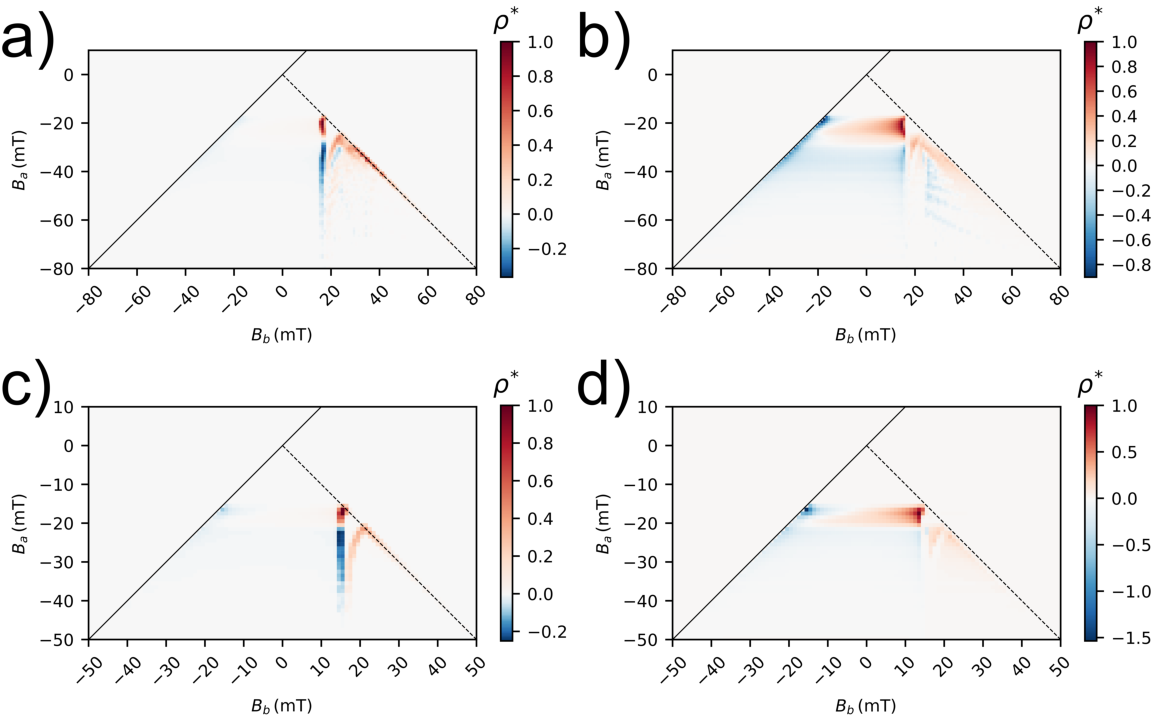
\includegraphics[width=\textwidth]{research-2/figs/FIG03.pdf}
\caption[FORC distribution heat maps (dipolar model)]{FORC distribution heat maps (normalised). a) Greigite and b) its purely reversible part; same for c,d) iron. Note the different scales for each material. Greigite ($K_1 < 0$) and iron ($K_1>0$) show very similar patterns. However, iron distintictively shows no negative sources, either reversible or irreversible, to the right of the negative-valued vertical ridge.}
\label{FIG_E03}
\end{figure}
\par
For iron (Figs. \ref{FIG_E03}(c--d)), the pattern formation is similar, if only with the position and width of the features changing. However, a fundamental difference is that for $K_1>0$ there is not an appreciable fraction of particles with hysteresis loops with more than two irreversible events. This is manifested in the FORC distribution by the absence of negative sources to the right of the negative vertical ridge.\par

FORC diagrams are usually presented as contour plots of the FORC distribution with higher values of the smoothing factor. The usual plotting axes are the transformed $B_c = (B_b - B_a)/2$, $B_u = (B_b + B_a)/2$; in this manner, FORC diagrams were calculated (Fig. \ref{FIG_E04}). The patterns show very similar pattern formation. The higher SF has the effect not only of smoothing the distribution but can also make the reversible information more apparent, especially if nonlinear scales are used for the contours of lower values.
\begin{figure}
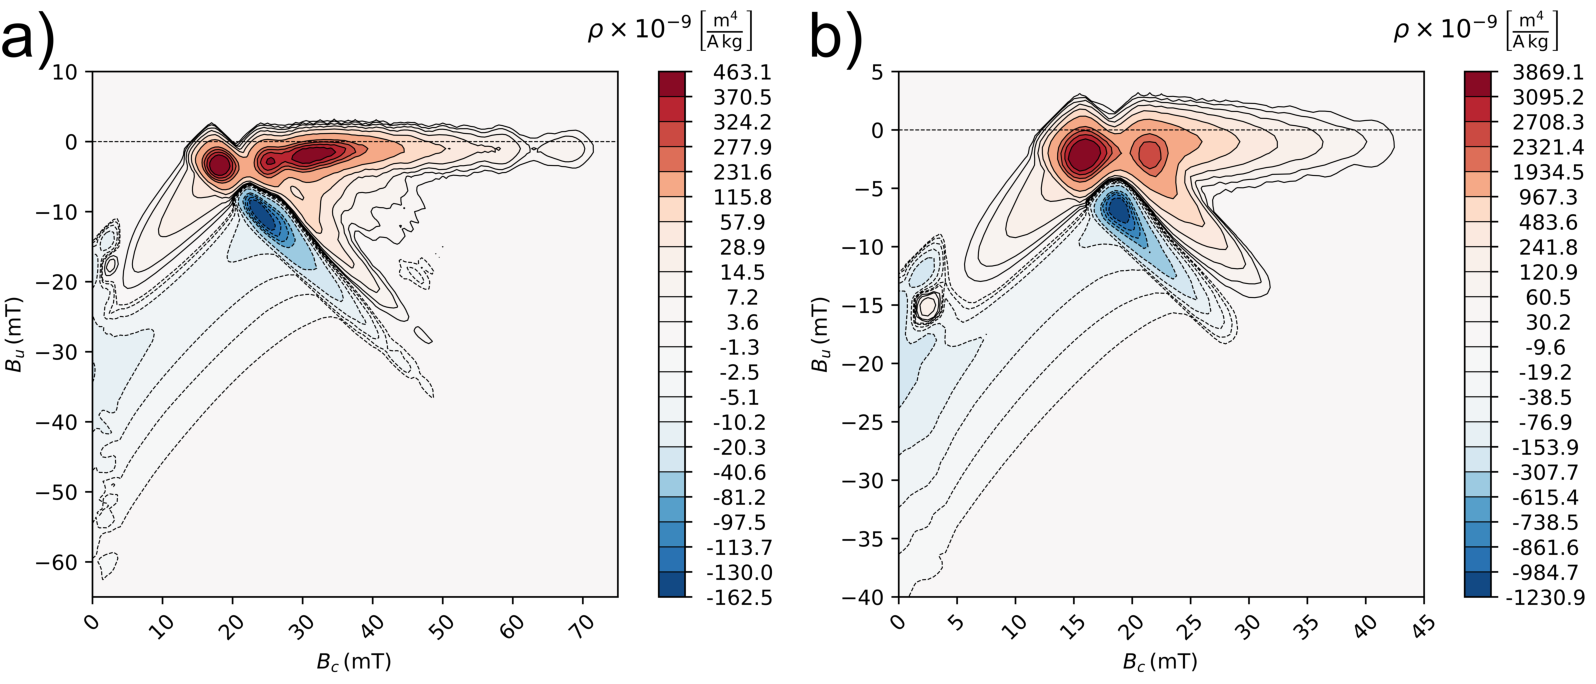
\includegraphics[width=\textwidth]{research-2/figs/FIG04.pdf}
\caption[FORC diagrams (dipolar model)]{The FORC diagrams. a) Greigite (SF=4); b) iron (SF=4). Note the different scales. The pattern formations are very similar in overall shape. Contour lines are plotted using a combination of linear and nonlinear scales at $(2^{-7},\ldots, 2^{-1},0.6, 0.7, 0.8)\times (\max (\rho), \min (\rho))$.}
\label{FIG_E04}
\end{figure}
\par
The position of the features in the FORC diagrams is slightly offset from being centered around the $B_u=0$ axis. This has been observed before in both measured and modelled FORC diagrams. \citet{Newell2005} attributes this to either a numerical artifact introduced by the least-square fitting-type calculation of the FORC distribution or to thermal effects. However, at least in this study, this should be attributed to the reversible contributions accumulating just below the central ridge.\par

The FORC diagrams obtained here for noninteracting ensembles of SD particles with cubic MCA shows good agreement with the weakly interacting ensembles of \citet{Harrison2014} as far as overall shape, e.g., the tilted negative ridge (Fig. \ref{FIG_E04}). The elongated, negative-valued ridge is highly significative and related to the presence of intermediate states, i.e., more than one irreversible event along the hysteresis curve. Uniaxial particles cannot produce this type of FORC distribution sources, so this is possibly a unique magnetic fingerprint of noninteracting to weakly interacting, coherent-rotating SD particles with cubic MCA. The tilted negative ridge has been observed before in FORC measurements of synthetic and natural greigite samples \citep{Roberts2011} and meteoritic samples \citep{Acton2007}.\par

FORC diagrams are usually presented normalised and their interpretation is usually qualitative. We find that iron produces much stronger FORC distribution sources per mass unit than greigite (Fig. \ref{FIG_E04}). It is possible that the strength of the negative ridge can be used in the future for quantitative studies, but more work is needed in this direction.\par

\section{Conclusion}
The FORC distribution and diagram of noninteracting dispersions of SD particles with cubic MCA was calculated. The numerical algorithm was found to be robust and fast. It is important that the minimiser takes sensible steps in order to closely follow the gradient-descent direction and not end up in local energy minima across energy barriers; the Armijo-Goldstein control parameters used in this study ensure these conditions.\par

The mechanism behind the pattern formation on the FORC diagram of dilute dispersions of SD particles with cubic MCA was identified. The FORC signals due to the reversible and irreversible motions were determined. The FORC diagram pattern of noninteracting to weakly interacting, cubic MCA SD particle ensembles are robust, which supports the idea of FORC diagram use for the identification of a noninteracting to weakly-interacting fraction of SD particles with cubic MCA.\par

The elongated negative ridge can possibly be interpreted as the FORC signal unique to noninteracting to weakly-interacting SD cubic MCA particles. Identification of this signal should be straightforward since its noninteracting nature means that it is essentially additive. Experimental work with dilute dispersions of fine particles of greigite, iron, magnetite or other magnetic minerals with a cubic MCA can provide answers to some of these open questions.\par

%%%% REFERENCES
%\renewcommand\bibname{{References}}
%\bibliographystyle{elsarticle-harv}
%\bibliography{references}


%\chapter{Magnetic vortex effects on first-order reversal curve (FORC) diagrams for greigite dispersions}
\label{ch:res-3}
\fancyhead[L]{Chapter 4. Single-vortex effects on FORC diagrams}
\fancyhead[C]{}
\fancyhead[R]{}
\fancyfoot[C]{\thepage}

This Chapter is submitted for publication as Valdez-Grijalva, M. A., Muxworthy, A. R., Williams, W., \'O Conbhu\'i, P., Nagy, L., Roberts, A. P., Heslop, D., 2018. Magnetic vortex effects on first-order reversal curve (FORC) diagrams for greigite dispersions. Earth Planet. Sci. Lett., in review.

\section*{Abstract}
First-order reversal curve (FORC) diagrams are used increasingly in geophysics for magnetic domain state identification. The domain state of a magnetic particle is highly sensitive to particle size, so FORC diagrams provide a measure of magnetic particles size distributions. However, the FORC signal of particles with nonuniform magnetisations, which are the main carrier of natural remanent magnetisations in many systems, is still poorly understood. In this study, the properties of non-interacting, randomly oriented dispersions of greigite (Fe$_3$S$_4$) in the uniform single-domain (SD) to non-uniform single-vortex (SV) size range are investigated via micromagnetic calculations. Signals for SD particles ($<50\nm$) are found to be in excellent agreement with previous SD coherent-rotation studies. A transitional range from $\roughly$50$\nm$ to $\roughly$70$\nm$ is identified for which a mixture of SD and SV behaviour produces complex FORC diagrams. Particles $> \roughly 70\nm$ have purely SV behaviour with the remanent state for all particles in the ensemble represented by the vortex state. It is found that for SV ensembles the FORC diagram provides a map of vortex nucleation and annihilation fields and that the FORC distribution peak should not be interpreted simply as the coercivity of the sample, but as a vortex annihilation field on the path to saturation.\par

\section{Introduction}
First-order reversal curve (FORC) diagrams are a powerful tool in rock magnetic studies, which allow mineral and domain state identification as well as quantification of magnetostatic interactions among particles \citep{Pike1999,Roberts2000,Roberts2014,Dumas2007,Egli2010}. As such, they have been the subject of numerical studies aimed at relating the behaviour of individual magnetic particles and small assemblages to experimental bulk properties \citep{Pike1999,Carvallo2003,Carvallo2006,Muxworthy2004,Muxworthy2005,Newell2005,Harrison2014,ValdezGrijalva2017,Roberts2017}.\par

With the exceptions of \citet{Carvallo2003} and \citet{Roberts2017}, all of these numerical studies have concentrated on FORC diagrams for ideal, uniformly magnetised single-domain (SD) particles. They have shown that uniaxial SD particles produce patterns in FORC diagrams \citep{Muxworthy2004,Newell2005,Harrison2014}, that are distinct from those for SD materials with cubic anisotropy \citep{Muxworthy2004,Harrison2014,ValdezGrijalva2017}. However, it is well-documented that most natural systems have magnetic signals dominated by larger grains with more complex magnetic domain states \citep{Dunlop,Roberts2017}. Grains just above the SD threshold size (e.g., $\roughly 64 \nm$ for equidimensional magnetite, $\roughly 54 \nm$ for greigite), are typically in a single-vortex (SV) state. The SV state dominates magnetic structures over an order of magnitude of size variations \citep{Nagy2017, ValdezGrijalva2017B}, which is much wider than the stable SD size range. SV grains have recently been found to be geologically meta-stable and retain relatively high remanences \citep{Almeida2014,Nagy2017, ValdezGrijalva2017B}.\par

Previous experimental studies on nano-patterned arrays of SV particles \citep{Pike1999B,Dumas2007} found that FORC diagrams are significatively more complex than for SD signals, with complex off-axis ``butterfly'' patterns that are related to vortex nucleation/annihilation processes. However, it is difficult to relate the behaviour of 2D nano-patterned arrays to the behaviour of natural particle systems found in geological samples. In natural samples, particles with varying size and orientation are dispersed in 3 dimensions. Thus, it is important to understand the contribution of dispersions of randomly aligned SV particles to FORC diagrams. Numerical modelling can aid the study of such systems. \citet{Carvallo2003} used a finite-difference model to calculate the FORC distributions of SV magnetite particles; however, that study primarily examined the effects of interactions between small clusters of cubic grains, and neither random particle distributions nor realistc grain morphologies were included.\par

In this study, we employ a micromagnetic finite element method (FEM) to obtain FORC diagrams for non-interacting ensembles of SD and SV greigite (Fe$_3$S$_4$). Greigite is the iron-sulphide counterpart to magnetite. Recent interest in greigite comes from both its promising properties for material science \citep{Li2014} and the abundance of this mineral in sedimentary rocks for Earth science \citep{Roberts2011}. FORC diagrams are often used to help identify greigite. The relatively high anisotropy of greigite means that the behaviour of this mineral is representative of cubic-anisotropic ferri- and ferro- magnets like magnetite and iron. We calculate FORC diagrams for simulations of non-interacting dispersions of randomly oriented greigite with sizes 30--80$\nm$; this size range covers the SD--SV threshold \citep{ValdezGrijalva2017B}. Simulations are carried out on an ensemble of 500 particles with random orientations. The unstructured discretisation of FEMs allows us to study realistic greigite particle shapes as observed in nature. We determine the onset of SV behaviour and its consequences for FORC diagram interpretation.\par
%-----------------------------------------------------

\section{Methods}
\subsection{The micromagnetic algorithm}
A ferromagnetic material{\textemdash}neglecting thermal and magnetostrictive effects{\textemdash}has a Gibbs free-energy functional given by \citep{Brown}:
\begin{equation}
E_\text{G} = \int_{\Omega} (\phi_{\text{exchange}} + \phi_{\text{anisotropy}} + \phi_{\text{stray}} + \phi_{\text{external}})\,\text{d}^3 \boldsymbol{r},
\end{equation}
where $\Omega$ is the ferromagnetic volume. Here,
\begin{equation}
\phi_{\text{exchange}}=A|\nabla\boldsymbol{m}|^2,
\end{equation}
where $\boldsymbol{m}$ is the reduced magnetisation vector and $A$ the exchange stiffness constant, provides an expression for the energy density due to quantum-mechanical exchange forces \citep{Landau1935}.\par
\begin{equation}
\phi_{\text{anisotropy}}=\frac{K_1}{2}\sum_{i\neq j}\gamma_i^2\gamma_j^2 + K_2\prod_i\gamma_i^2,
\end{equation}
where $\gamma_i$ represent the direction cosines and $K_1$ and $K_2$ the first and second magnetocrystalline anisotropy (MCA) constants, is the MCA energy density in the cubic anisotropy system. In terms of the reduced magnetisation vector components, this becomes:
\begin{equation}
\phi_{\text{anisotropy}}=K_1(m_x^2m_y^2+m_y^2m_z^2+m_z^2m_x^2),
\end{equation}
where $K_2$ is neglected because $K_1$ is the dominant term at room temperature. The magnetostatic self-energy density is given by:
\begin{equation}
\phi_{\text{stray}}=-\frac{\mu_0M_\text{S}}{2}\boldsymbol{m}\cdot\boldsymbol{H}_{\text{stray}},
\end{equation}
where $\boldsymbol{H}_{\text{stray}}$ is the stray field produced by the ferromagnetic body and $M_\text{S}$ is the saturation magnetisation. Finally, the energy density due to an external magnetic field $\boldsymbol{H}_{\text{external}}$ is:
\begin{equation}
\phi_{\text{external}}=-\mu_0M_\text{S}\boldsymbol{m}\cdot\boldsymbol{H}_{\text{external}}.
\end{equation}\par

Such magnetic particle systems will be driven spontaneously toward an equilibrium state with a locally minimal magnetic Gibbs free-energy \citep{Brown}. In this study we utilise a modified gradient descent method to find the equilibrium magnetisation \citep{OConbhui2017}.\par

Discretisation of the spatial domain is achieved by decomposing the volume into tetrahedral elements. This allows modelling of particles with arbitrary geometries. To model accurately nonuniform magnetisations, spatial discretisation in the model should be smaller than the exchange length $l_\text{exch.} = \sqrt{2A/\mu_0M_\text{S}^2}$ \citep{Rave1998}, which for greigite is $l_\text{exch.} \approx 6.6\, \text{nm}$; a maximum element size of 5$\nm$ was used for all simulations. The non-local problem of calculating the stray field is resolved by a hybrid finite-element/boundary-element method (BEM) formulation \citep{Fredkin1990}.\par

The magnetic parameters of greigite used in this investigation are: the saturation magnetisation $M_\text{S}= 2.7 \times 10^5\,\text{A/m}$ \citep{Li2014}; the exchange stiffness constant $A=2\times10^{-12}\,\text{J}/\text{m}$ \citep{Chang2008}; and the first MCA constant $K_1=-1.7\times10^4\,\text{J}/\text{m}^3$ \citep{Winklhofer2014}. This set of parameters has been used in recent numerical studies of greigite \citep{ValdezGrijalva2017B,ValdezGrijalva2017}.\par

\subsection{The FORC model}
FORC diagrams are constructed from a class of partial hysteresis curves called first-order reversal curves \citep{Mayergoyz1986}, each starting at a value $B_a$ of the applied field along the main hysteresis branch and tracing the magnetisation as the field $B_b$ is increased to saturation. A magnetisation function on two variables $M=M(B_a, B_b)$ is thus obtained. The FORC distribution $\rho$ is then defined as \citep{Roberts2000}:
{\par\nobreak\noindent}
\begin{equation}
\rho=-\frac{1}{2}\frac{\partial^2 M}{\partial H_a \partial H_b}=-\frac{\mu_0^2}{2}\frac{\partial^2 M}{\partial B_a \partial B_b},
\end{equation}
where $\mu_0$ is the magnetic constant (or vacuum permeability) and $H=B/\mu_0$.\par

Once $M(B_a, B_b)$ is obtained, calculation of $\rho(B_a, B_b)$ is done by least-squares fitting of a degree 2 polynomial surface $a_0 + a_1 B_a + a_2 B_b + a_3 B_a B_b + a_4 B_a^2 + a_5 B_b^2 + \text{error} = M(B_a,B_b)$ on a subgrid of $M(B_a, B_b)$ centered around $(B_a, B_b)$ as determined by the so-called smoothing factor (SF) and including (2$\times$SF + 1)$^2$ points; the value of $\rho$ is then simply $-\mu_0^2 a_3/2$ \citep{Pike1999}. FORC diagrams are usually presented with rotated axes $B_c=(B_b - B_a)/2$, $B_u=(B_b + B_a)/2$.\par

Distributions with random orientation of magnetic particles with respect to the applied field were determined by taking 500 field orientations from a sector of the unit sphere (Fig. \ref{FIG_C4_01}). We use 500 field orientations as a workable compromise between accuracy and calculation speed. Also, for each particle/field-orientation, the hysteresis curve consists mostly of reversible motion of the magnetisation; thus, we only need to calculate the main branch of the hysteresis loop and the few reversal curves starting at the different switching fields along the main branch \citep{ValdezGrijalva2017}. The switching events are identified either by an abrupt change in the scalar net magnetisation $\Delta (M/M_\text{S})>0.1$ or a rotation of the net magnetisation vector larger than 5 degrees. These simplifications reduce vastly the number of calculations needed without loss of important information. The external-field rate of change for all models was 1$\mT$ with a saturation field of 250$\mT$, so that 501 reversal curves were calculated for each particle/field-orientation.
\begin{figure}
\centering
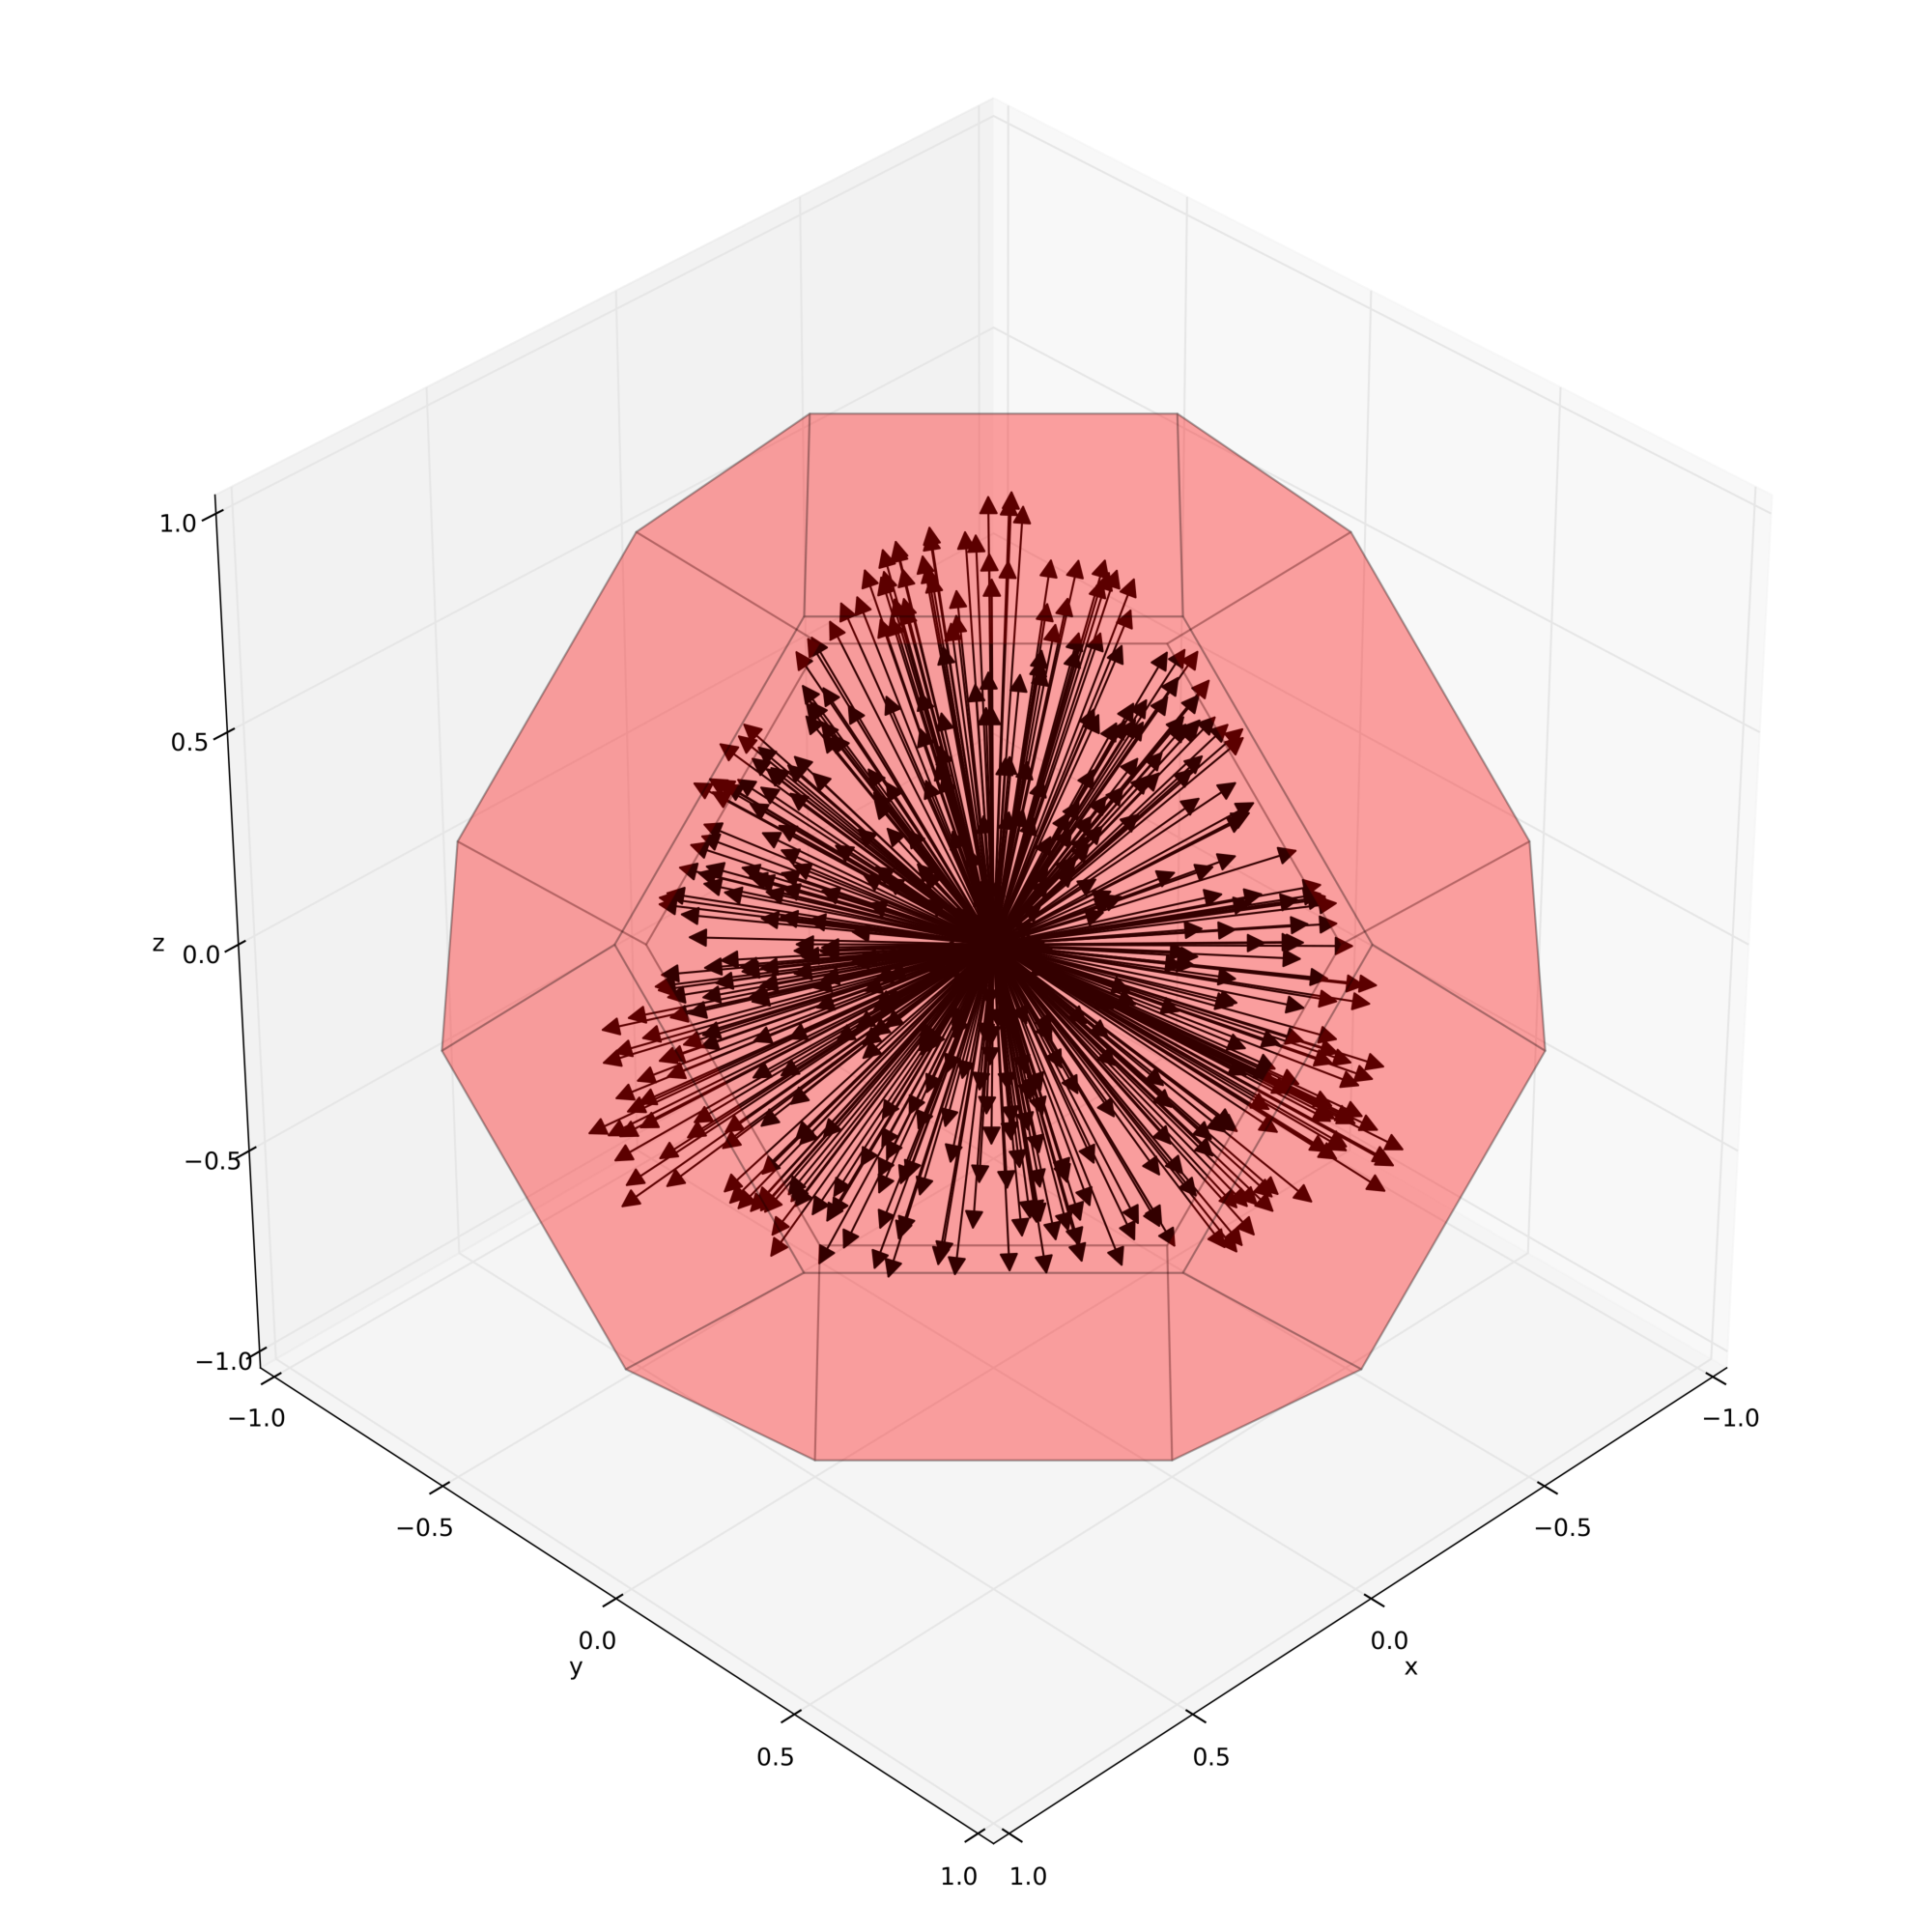
\includegraphics[width=\textwidth]{research-3/figs/FIG_01.pdf}
\caption[Model geometry and field orientations]{Model geometry and field orientations. The most common morphology for authigenic greigite is truncated octahedral. To avoid the high density of field orientations necessary near the sphere poles when using a regular grid, 500 random field orientations (arrows) were chosen from a uniform distribution over a sector of the unit sphere. The periodicity of the magnetocrystalline anisotropy and particle symmetry allow modelling of the effects of field orientations on only a sector of the sphere without loss of generality.}
\label{FIG_C4_01}
\end{figure}\par

Scanning electron and transmission electron micrographs of naturally occurring greigite samples \citep{Snowball1997,Vasiliev2008,Roberts2015} reveal that greigite tends to grow authigenically as well-defined regular truncated octahedral particles. Micromagnetic calculations for truncated octahedral greigite particles indicate that the SD--SV threshold occurs at $\roughly 54\nm$ \citep{ValdezGrijalva2017B}. In this study we model FORC diagrams for non-interacting ensembles of truncated octahedral greigite particles sized 30--80$\nm$ (where size is normalised to the volume of a cube) at 2$\nm$ size intervales. This range is chosen because it spans the transition from SD to SV behaviour.\par

%-----------------------------------------------------

\section{Results}
For ensembles with SD particles $<50\nm$, hysteresis behaviour is dominated by coherent rotation (Fig. \ref{FIG_C4_02}). This is seen by comparing FORC diagrams for these ensembles (Fig. \ref{FIG_C4_02}b) with those of idealised SD (effectively a single magnetic dipole), coherently rotating greigite particles (Fig. \ref{FIG_C4_02}a) determined using the method outlined in \citet{ValdezGrijalva2017}. Diagrams for particles $<50\nm$ obtained with the micromagnetic algorithm (Fig. \ref{FIG_C4_02}b) are offset $\roughly 3\mT$ to the left compared to the dipole model (Fig. \ref{FIG_C4_02}a); lower coercivities due to the micromagnetic algorithm, which includes flowering (small deviations from a perfect SD structure) as a result of magnetostatic self-interaction effects, account for this effect.
\begin{figure}
\centering
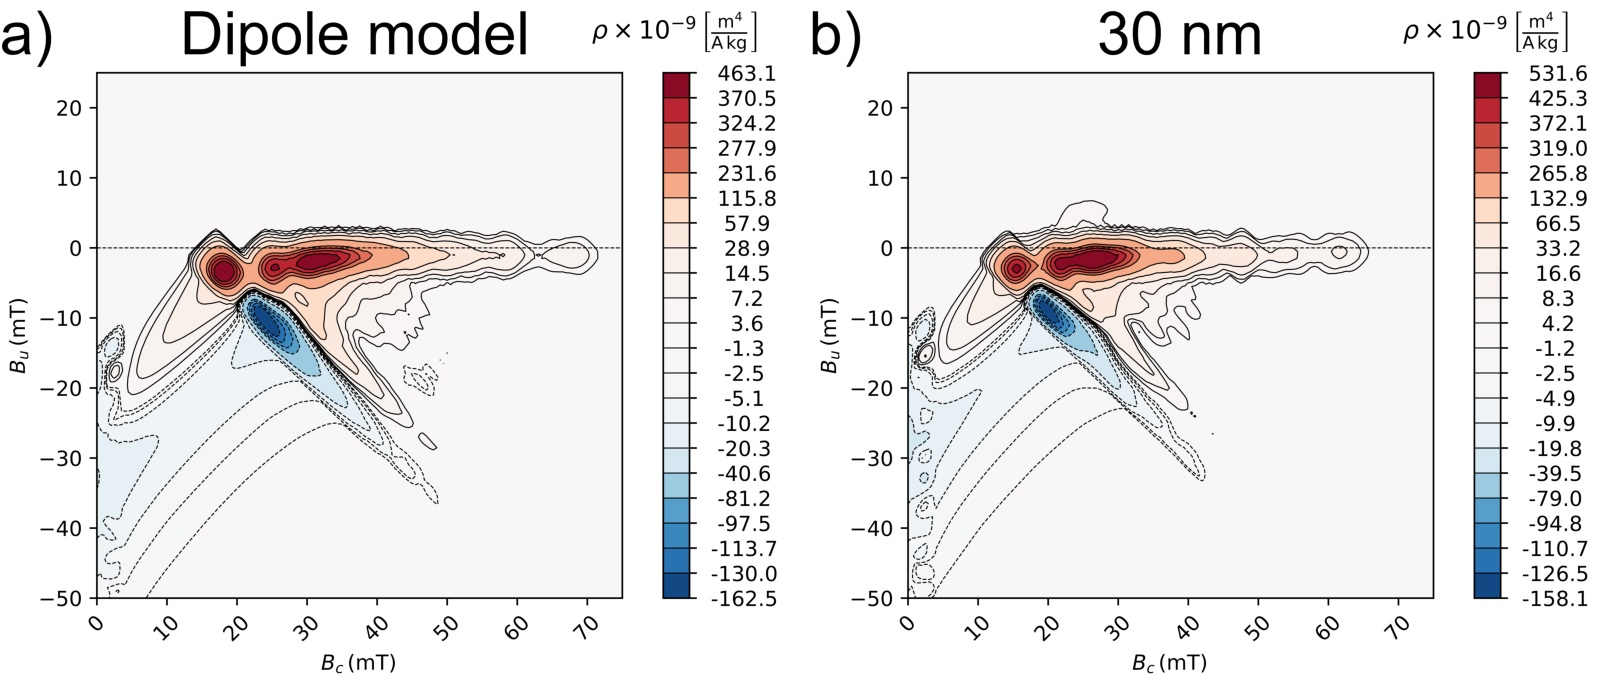
\includegraphics[width=\textwidth]{research-3/figs/FIG_02.pdf}
\caption[Comparison between dipole and micromagnetic model]{Comparison between FORC diagrams produced with dipole and micromagnetic models. a) Dipole model; FORC diagram (SF=4) for a non-interacting ensemble of idealised (size-independent) SD greigite particles obtained using the model of \citet{ValdezGrijalva2017}. b) Micromagnetic model; FORC diagram (SF=4) for a non-interacting ensemble of 30$\nm$ truncated octahedral greigite particles. Up to 48$\nm$, the FORC diagram is that of an ensemble of coherently rotating SD moments. For particles larger than 48$\nm$, magnetic vortex effects become important. Dashed contour lines denote negative $\rho$ values.}
\label{FIG_C4_02}
\end{figure}\par

Particles with cubic anisotropy have hysteresis behaviour that departs from that observed from the simple hysteron consisting of one plus and one minus magnetisation states. There exist intermediate easy axis states along hysteresis curves for the SD state \citep{ValdezGrijalva2017}. The tilted, elongated, negative-valued ridge (Fig. \ref{FIG_C4_02}) is a consequence of the availability of multiple hysteresis main branches caused by the cubic anisotropy. This negative-valued ridge is produced by the fraction of particles with a hard axis aligned closely with the applied field. These particles have the lowest switching fields: from the plus-state to an intermediate state at $B= B^{+}_{*}$ and from the intermediate state to the minus-state at $B=B^{*}_{-}$. Reversal curves with $B^{*}_{-} < B_a < B^{+}_{*}$ experience a sharp upward discontinuity at $B_b = B^{*}_{+} \leq |B^{+}_{*}|$ when hard-aligned particles return to the plus-state from their intermediate states. The combination of this type of irreversible event in hard-aligned particles causes the local peak at $B_c\approx 15 \mT, B_u\approx {-}3\mT$ (Fig. \ref{FIG_C4_02}b). For reversal curves with $B_a < B^{*}_{-}$, hard-aligned particles are initially in the minus-state and undergo irreversible rotation to an intermediate state on the path to positive saturation at $B=B^{-}_{*} = |B^{+}_{*}|$ due to the symmetry of the particles and the lack of magnetostatic interactions. The combination of these irreversible events causes a negative FORC distribution response at $B_a=B^{*}_{-}, B_b=B^{*}_{+}$. The sum effect of this type of response for many particles with a distribution of switching fields produces the elongated negative contribution observed in all SD ensembles, roughly along the line segment connecting ($B_c=18\mT,B_u=-6\mT$) with ($B_c=42\mT,B_u=-30\mT$).\par

The fraction of particles with easy axis alignment close to the applied field orientation exhibits hysteron-like behaviour, i.e., just two switching fields: from the plus-state to the minus-state $B^{+}_{-}$ and \textit{vice versa} $B^{-}_{+}$. The lack of interactions and the symmetry of particles in our simulations ensure that $|B^{+}_{-}| = B^{+}_{-}$. Thus, this fraction of particles produces FORC distribution responses at $B_a=B^{+}_{-}, B_b=B^{-}_{+}$. These types of irreversible responses accumulate on the line $B_a=-B_b$; they account for the most drastic changes in the magnetisation of the ensemble and, thus, account for the high slopes around the coercive field of the sample. This makes the position of the FORC diagram peak coincide with the coercivity of $B_\text{C}\approx 24\mT$ for SD ensembles.\par

Particles with size $d \geq 50\nm$ switch incoherently; that is, the FORC diagrams depart from coherent rotation behaviour associated with SD particles as the tight boomerang-shaped FORC diagram pattern exhibited by the SD greigite (Fig. \ref{FIG_C4_02}) becomes more fragmented (Fig. \ref{FIG_C4_03}). This change is driven initially by particles with hard axes close to the applied field nucleating hard-aligned vortices \citep{ValdezGrijalva2017B} as intermediate meta-stable states during hysteresis. Even though nucleation of hard-aligned vortices occurs in particles below the zero-field SD--SV threshold $d_0\approx 54\nm$ \citep{ValdezGrijalva2017B}, this is expected because vortex  nucleation greatly reduces the magnetic free-energy. A corollary of this is that a fraction of particles (with easy axis alignment close to the applied field) above the zero-field SD--SV threshold can remain in a SD state throughout hysteresis. These effects are due to distortion of the zero-field energy landscape by the applied field.
\begin{figure}
\centering
\includegraphics[width=\textwidth]{research-3/figs/FIG_03.pdf}
\caption[FORC diagrams with increasing vortex effects]{FORC diagrams with increasing vortex effects. SF=4 for all diagrams. a) 50$\nm$; b) 60$\nm$; c) 66$\nm$; and d) 76$\nm$. At these sizes, an ever larger fraction of the particle moments begin to switch with nonuniform magnetisations, i.e., vortex nucleation. At 76$\nm$ all particles are in the single vortex remanent state. Dashed contour lines denote negative $\rho$ values.}
\label{FIG_C4_03}
\end{figure}\par

An appreciable positive source in the FORC distribution appears along the $B_u=0$ axis at $B_c\approx 52\mT$ (the $B_c$ axis is not to be confused with the coercivity $B_\text{C}$) for ensembles with particles $\geq 54\nm$ (Fig. \ref{FIG_C4_04}, region 5); this contribution represents the annihilation of vortex states on the return to positive saturation. The elongated, negative ridge due to SD particles with cubic MCA and its corresponding symmetric positive response move to lower $(B_c, B_u)$ values (Fig. \ref{FIG_C4_04}, regions 1, 3) and the first responses for $B_u > 0$ begin to form (Fig. \ref{FIG_C4_04}, region 2); these are elongated features at 45$^{\circ}$ to the $B_u=0$ axis, which are different to the vertical widening usually attributed to magnetostatic interactions \citep{Pike1999,Muxworthy2004,Muxworthy2005}.
\begin{figure}
\centering
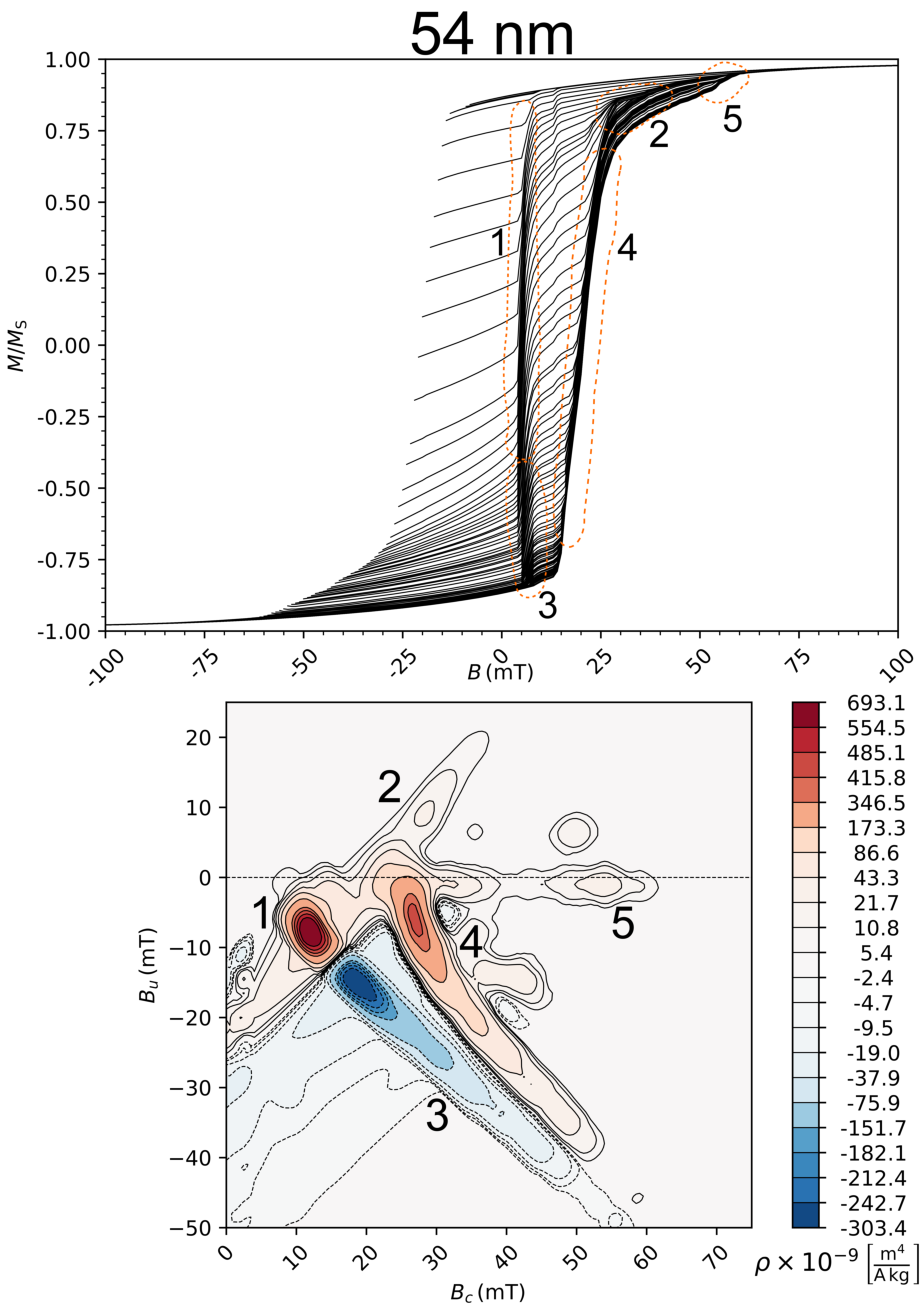
\includegraphics[width=0.9\textwidth]{research-3/figs/FIG_04.pdf}
\caption[FORC diagram and hysteresis curves of 54$\nm$-sized particles]{FORC diagram (SF=4) (bottom) and hysteresis curves (top) for 54$\nm$ particles. Annotations link the FORC diagram responses to the raw hysteresis curves. See text for details. Dashed contour lines on the FORC diagram denote negative $\rho$ values.}
\label{FIG_C4_04}
\end{figure}\par

For particles slightly below and above the SD--SV threshold $d_0$, vortex nucleation occurs only for negative applied field values, thus noticeable changes in the FORC diagrams (Fig. \ref{FIG_C4_03}a--c) are not evident in changes in the saturation remanence $M_\text{RS}$ to saturation magnetisation $M_\text{S}$ ratio up to 72$\nm$, whereas coercivity decreases sharply above 48$\nm$ (Fig. \ref{FIG_C4_05}b). The monotonically-decreasing coercivity trend is preserved up to 62$\nm$ when it rises from $B_{\text{C}}\approx 15 \mT$ to $\roughly 20 \mT$ for $d=68\nm$. With increasing size, coercivitiy decreases further, accompanied by a sharp decrease in $M_\text{RS}$ (Fig. \ref{FIG_C4_05}b). The drop in $M_\text{RS}$ is driven by particles nucleating vortices at $B_a>0$ for $d \geq 68\nm$. For $d \geq 76\nm$, all particles nucleate vortices so that the vortex state becomes the remanent magnetic domain state; this is reflected in the Day plot \citep{Day1977}, a scatter plot of the $M_\text{RS}/M_\text{S}$ ratio against the coercivity of remanence $B_\text{CR}$ (the field necessary to reduce the remanence to zero) to $B_\text{C}$ ratio, by particles 76$\nm$ and larger (Fig. \ref{FIG_C4_05}a), associated here with the SV state.
\begin{figure}
\centering
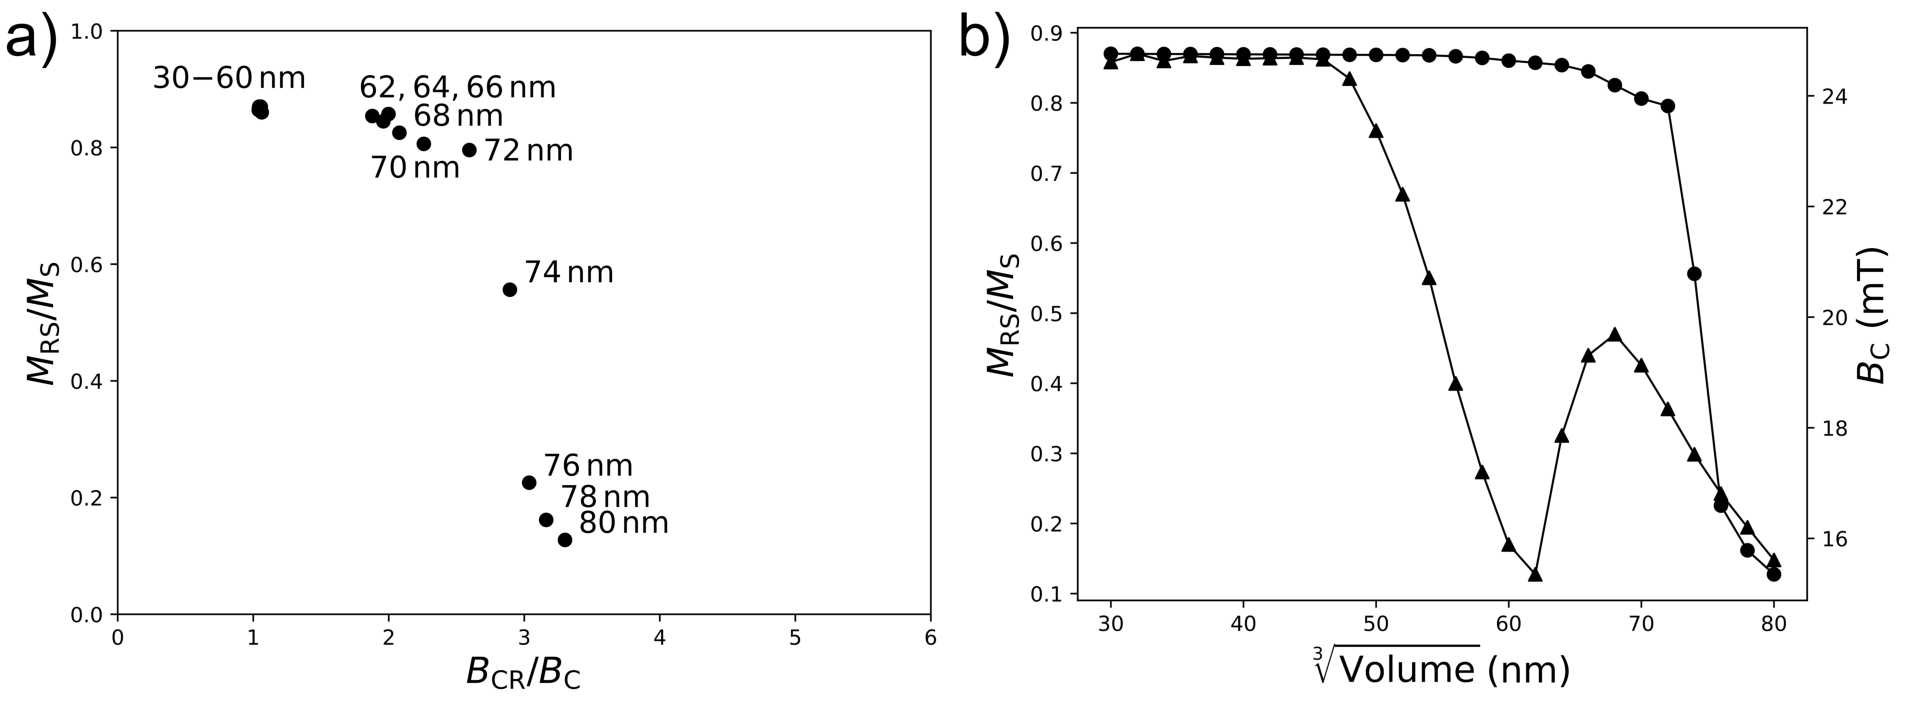
\includegraphics[width=\textwidth]{research-3/figs/FIG_05.pdf}
\caption[Day plot and remanence/coercivity against size]{Day plot and $M_\text{RS}/M_\text{S}$ and coercivity against particle size. a) The Day plot \citep{Day1977} contains data for SD particles up to 60$\nm$; however, we know from the micromagnetic solutions that vortices form from 50$\nm$ onward. Particles with size from 62 to 72$\nm$ plot in an unexpected region. Particles larger than 74$\nm$ plot with lower $M_\text{RS}/M_\text{S}$ and higher $B_\text{CR}/B_\text{C}$ values. b) Remanence (circles) and coercivity (triangles) versus particle size.}
\label{FIG_C4_05}
\end{figure}\par

Particles sized 62--72$\nm$ move away from the top left of the Day plot (Fig. \ref{FIG_C4_05}a) to a region with high remanence but larger $B_{\text{CR}}/B_{\text{C}}$ values. These sizes coincide with the anomalous coercivity increase for these sizes (Fig. \ref{FIG_C4_05}b). The increased coercivities can be explained by vortex nucleation, which causes hysteresis loops to become increasingly wasp-waisted (Fig. \ref{FIG_C4_06}) so that they cross the zero-magnetisation axis at increasing (absolute) values of the applied field strength. FORC diagrams for these sizes are the most complex of all those simulated here, and have a variety of features (Figs. \ref{FIG_C4_03}c, \ref{FIG_C4_06}) caused by the complex interplay of SV and SD effects. The elongated, negative ridge becomes more faint with increasing particle size, whereas the positive responses for $B_u>0$ become larger and move toward the $B_c=0$ axis with increasing size. Large, positive FORC responses for $B_u>0$ along the $B_c=0$ axis are expected for larger multi-domain (MD) grains \citep{Pike2001,Roberts2006}. The non-interacting nature of these ensembles means that the SD and SV FORC signals are linearly additive. Therefore, it is possible to discern the FORC responses due to SD (Fig. \ref{FIG_C4_06}, regions 3, 6) and SV particles (Fig. \ref{FIG_C4_06}, regions 1, 2, 4, 5, 7, 8).
\begin{figure}
\centering
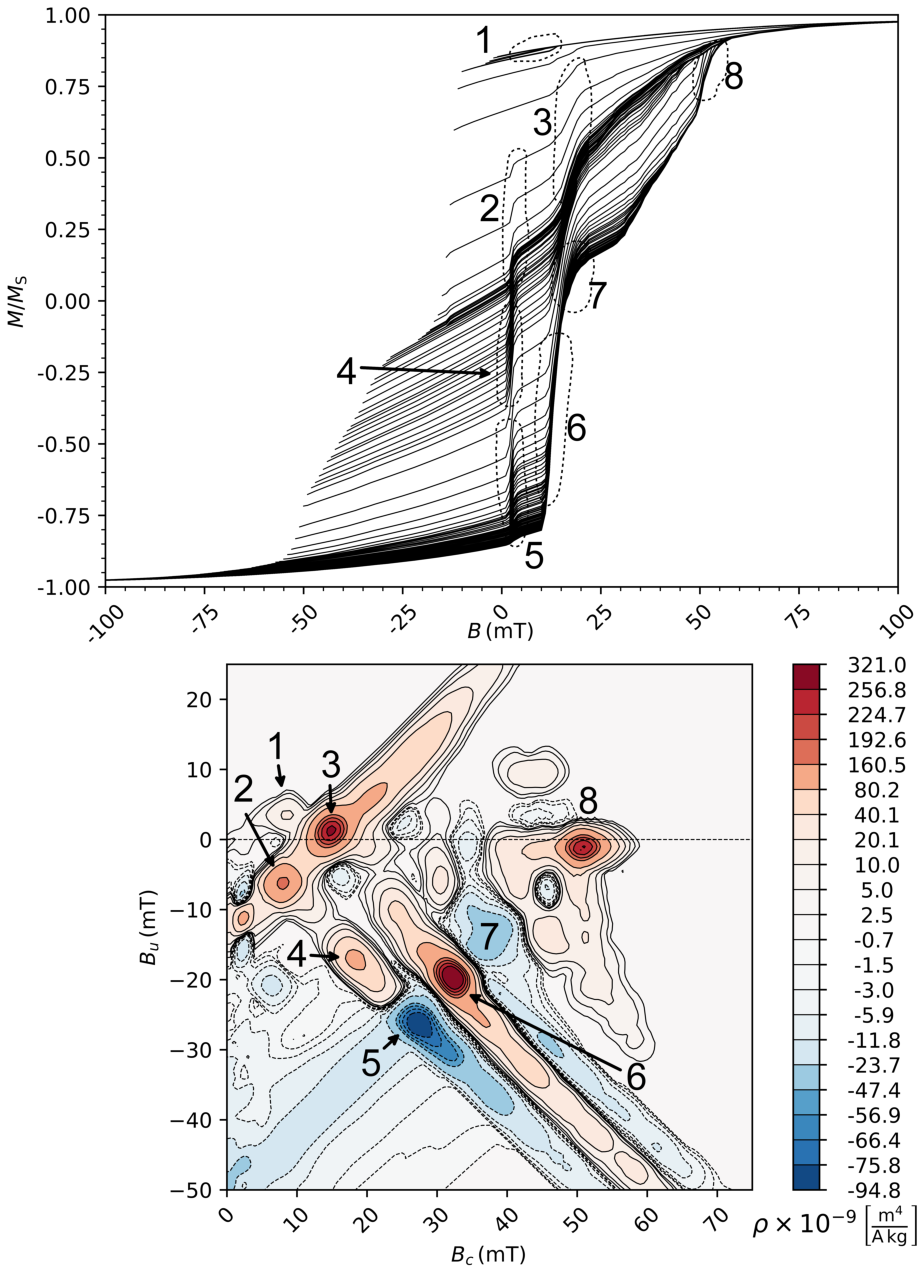
\includegraphics[width=0.9\textwidth]{research-3/figs/FIG_06.pdf}
\caption[FORC diagram and hysteresis curves of 62$\nm$-sized particles]{FORC diagram (SF=4) (bottom) and hysteresis curves (top) for 62$\nm$ particles. Annotations link the FORC diagram responses to the raw hysteresis curves. See text for details. Dashed contour lines on the FORC diagram denote negative $\rho$ values.}
\label{FIG_C4_06}
\end{figure}\par

The elongated, negative ridge typical of SD particles with cubic MCA \citep{ValdezGrijalva2017} disappears for particles $\geq 76 \nm$ (Fig. \ref{FIG_C4_03}d). A circular, negative feature centered roughly at ($B_c=8 \mT, B_u={-}8\mT$) becomes larger and of a magnitude comparable to the largest positive reponses. For $d=76$ and 78$\nm$ the negative response has a larger absolute value than the distribution peak (Fig. \ref{FIG_C4_03}d). For the 80$\nm$ particle model, a faint negative response appears centered roughly at ($B_c=40 \mT, B_u={-}12\mT$) (Fig. \ref{FIG_C4_07}, region 6). Fig. \ref{FIG_C4_07} represents the contribution of purely SV particles, that is, ensembles of particles that are all in a SV remanent state. It is logical that this FORC diagram is somewhat less complex than those for ensembles with a fraction of particles still in the SD state as well as some in the SV state; the difference is due to the field angle relative to particle orientation, as has also been shown by \citet{Roberts2017} for magnetite.
\begin{figure}
\centering
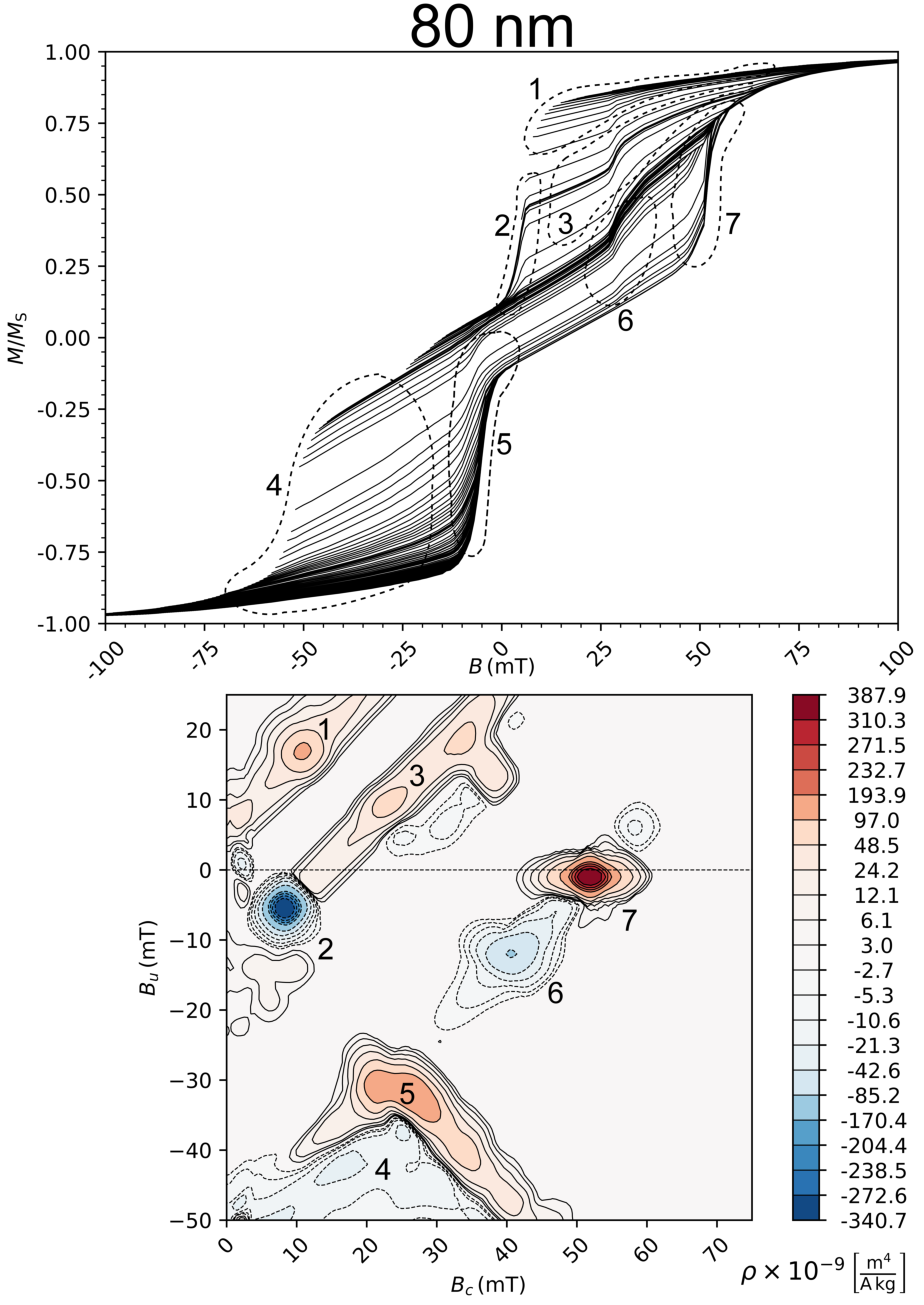
\includegraphics[width=0.9\textwidth]{research-3/figs/FIG_07.pdf}
\caption[FORC diagram and hysteresis curves of 80$\nm$-sized particles]{FORC diagram (SF=4) (bottom) and hysteresis curves (top) for 80$\nm$ particles. Annotations link the FORC diagram responses to the raw hysteresis curves. See text for details. Dashed contour lines on the FORC diagram denote negative $\rho$ values.}
\label{FIG_C4_07}
\end{figure}\par

Particles with hard axes aligned closely with the applied field nucleate hard-aligned vortices at high applied field values (Figs. \ref{FIG_C4_hardaxis}a, \ref{FIG_C4_08}); as the field decreases below $\roughly 12\mT$ these vortices rotate irreversibly to an easy axis alignment (Fig. \ref{FIG_C4_hardaxis}b). As the field is increased on reversal curves with $\roughly 0\mT \leq B_a \leq \roughly 12\mT$ these vortices switch irreversibly back to a hard alignment at $B_b\approx 28 \mT$ to create a local peak at $B_c \approx 12 \mT,\, B_u \approx 16 \mT$ (Fig. \ref{FIG_C4_07}, region 1); this is manifested in the raw hysteresis data by the smoothed discontinuity at $B\approx 28 \mT$ whereas the reversible motion traced by the reversal curves around this region accounts for the tilted, elongated response surrounding the local peak.
\begin{figure}
\centering
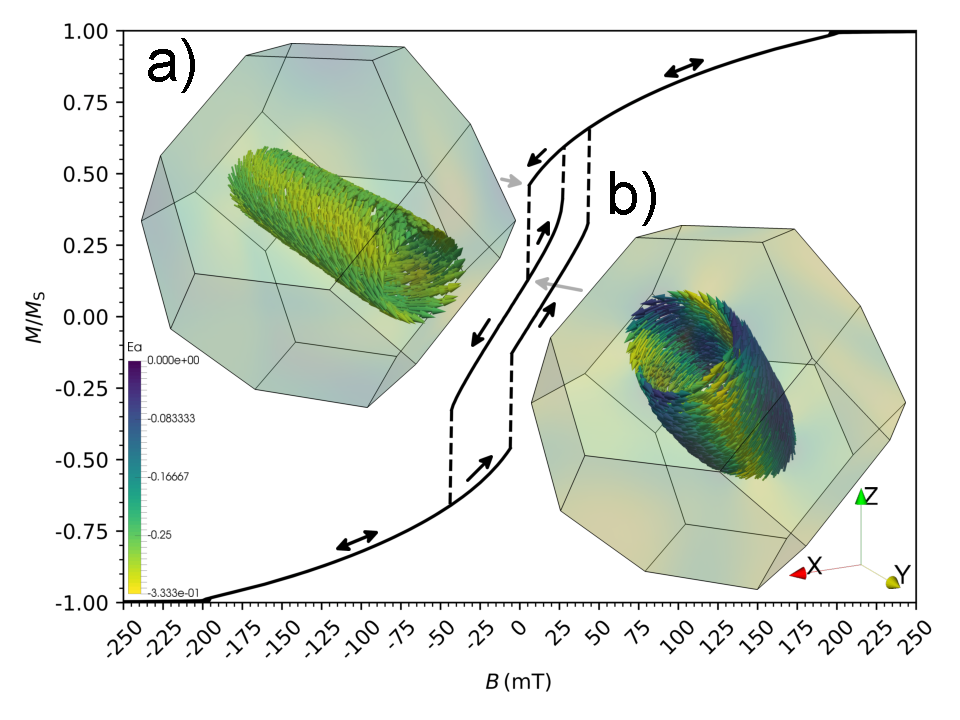
\includegraphics[width=\textwidth]{research-3/figs/BMforcs_080nm_015_edit.pdf}
\caption[Hysteresis of 80$\nm$-sized particle with applied field along a hard axis]{Hysteresis main branch, reversal curves and micromagnetic solutions of 80$\nm$-sized particle with applied field along a hard $<$010$>$ axis. A hard-aligned vortex nucleates at high values of the applied field with a negligible net magnetisation change and therefore negligible contribution to the FORC distribution. The vortex is stable as the field is decreased down to 6$\mT$ (a). Decreasing the field to 5$\mT$ causes the vortex core to rotate irreversibly to an easy $<$111$>$ axis (b). A reversal curve starting at this switching value rotates back to the hard axis alignment when the field is increased to 28$\mT$. The vortex cores are highlighted by their helicity ($m \cdot \nabla \times m$) and coloured according to the anisotropy energy.}
\label{FIG_C4_hardaxis}
\end{figure}\par

During hysteresis, as the remanent state is approached, all particles $\geq 76 \nm$ have nucleated vortices: particles with easy axis alignment close to the applied field directly nucleate an easy-aligned vortex while the rest nucleate vortices initially oriented along hard $<$100$>$ or $<$110$>$ directions (Fig. \ref{FIG_C4_08}b), which rotate irreversibly to an easy axis alignment as the field approaches zero. The latter fraction of particles then undergo irreversible rotations to intermediate positions for $\roughly{-}10\mT \leq B \leq \roughly{-}20\mT$. For FORCs with $\roughly{-}10\mT \leq B_a \leq \roughly{-}20\mT$, these vortices rotate back to the initial easy axis alignment at $B_b\approx 4 \mT$. A combination of these irreversible events creates the lowest negative FORC response (Fig. \ref{FIG_C4_07}, region 2). A further applied field increase to $\roughly 30 \mT$ causes these vortices to switch to the initial hard position from which they nucleated. These events cause the tilted, elongated FORC response (Fig. \ref{FIG_C4_07}, region 3).\par

As the applied field decreases past $\roughly{-}52 \mT$, the vortices of particles with easy axis alignment close to the applied field annihilate (Fig. \ref{FIG_C4_08}). Reversal curves with $\roughly{-}80\mT \leq B_a \leq \roughly{-}52\mT$ trace lower slopes with decreasing $B_a$ due to the combined reversible motion of vortices and single domains; this is the source of the faint negative contribution for $B_u < \roughly 45 \mT$ (Fig. \ref{FIG_C4_07}, region 4). On increasing $B_b$ on these curves, nucleation of easy-aligned vortices occurs at $\roughly{-}5 \mT$ creating the boomerang-shaped response (Fig. \ref{FIG_C4_07}, region 5) that limits the faint negative response in region 4; this corresponds with the smoothed discontinuity in hysteresis curves as the field approaches zero from the left. Increasing the applied field to positive values causes the easy-aligned vortices of particles with hard axes close to the applied field to switch to hard alignments at $\roughly 28 \mT$, creating a negative FORC region (Fig. \ref{FIG_C4_07}, region 6). The distribution peak at region 7 (Fig. \ref{FIG_C4_07}) corresponds to the average annihilation field of the vortices on the reversal paths to positive saturation.
\begin{figure}
\centering
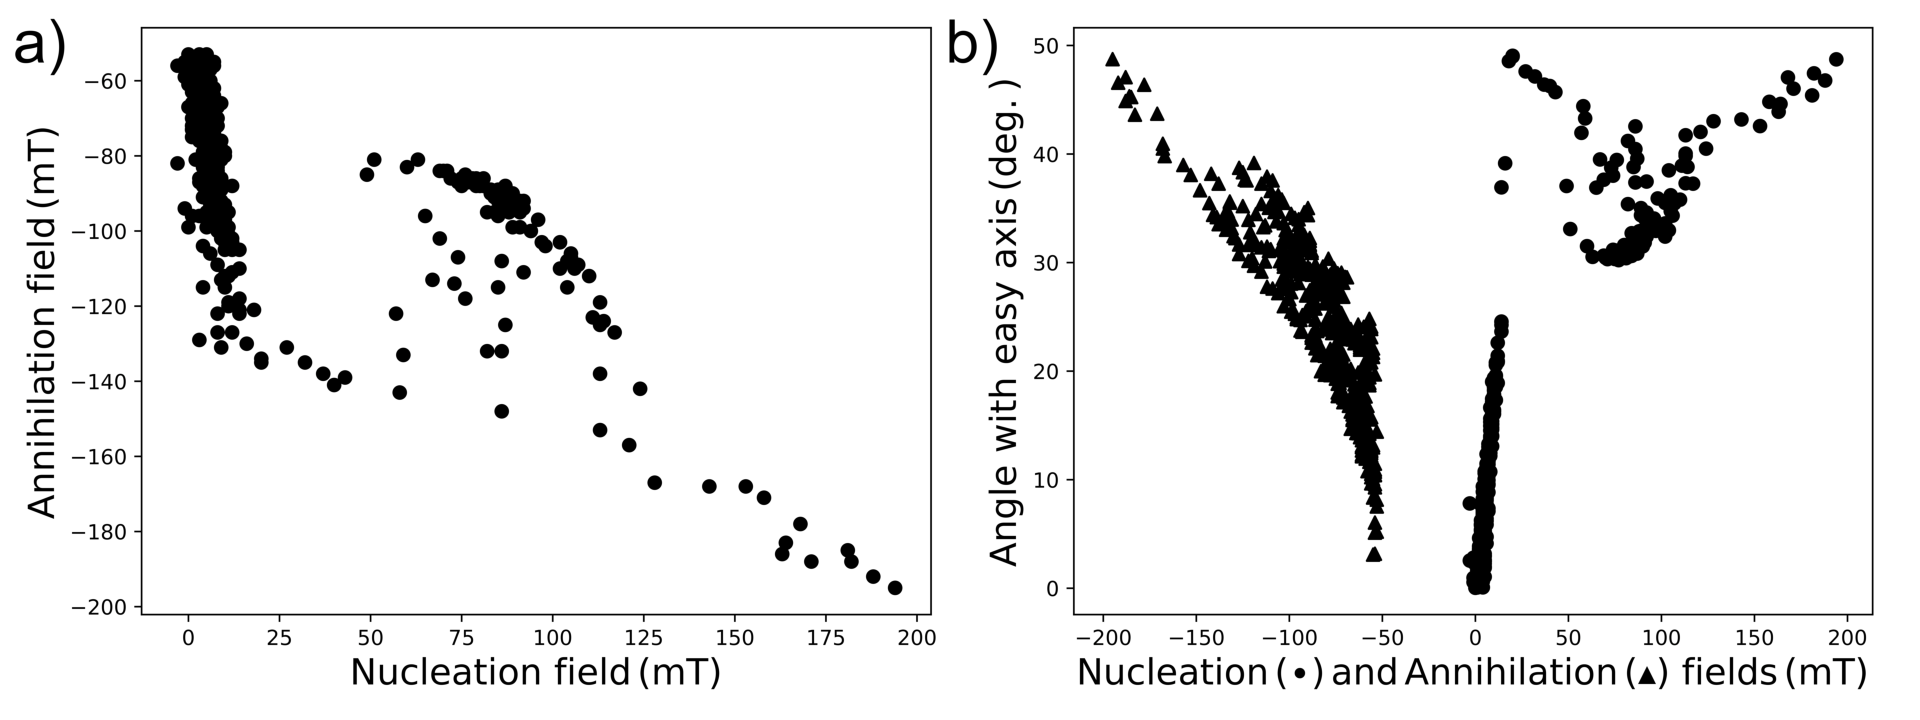
\includegraphics[width=\textwidth]{research-3/figs/FIG_08.pdf}
\caption[Vortex nucleation/annihilation fields]{Vortex nucleation and annihilation fields for the simulated particle ensembles. a) Scatter plot of annihilation field against nucleation field. Three trends are observed depending on whether the nucleated/annihilated vortex has an easy, hard or other alignment. b) Vortex core angle with an easy direction against the nucleation and annihilation fields (circles and triangles, respectively).}
\label{FIG_C4_08}
\end{figure}\par

There is a large spread in the vortex nucleation and annihilation fields (Fig. \ref{FIG_C4_08}). Particles with hard axis alignment close to the applied field nucleate hard-aligned vortices for fields as high as $\roughly 200 \mT$ and annihilate on the opposite side of the particle for equally high (absolute) values. However, these nucleation and annihilation events make a negligible contribution to the FORC diagram because the change in magnetisation of a particle nucleating/annihilating a hard-aligned vortex from/to a SD state can be as low as $1 \%$.\par

%-----------------------------------------------------
\section{Discussion}
Comparison of results for micromagnetic simulations presented here with the coherently rotating dipole model of \citet{ValdezGrijalva2017} indicates excellent agreement (Fig. \ref{FIG_C4_02}). This confirms the accuracy of our model using only 500 random field orientations instead of field orientations on a regular grid, which requires a high density of field orientations near the poles of the sphere. A FORC diagram for SD coherently rotating particles has the same general features as those obtained for weakly interacting SD particles with cubic MCA by \citet{Harrison2014}, i.e., a positive ridge along the $B_c$ axis, slightly offset toward $B_u<0$ values and a tilted, negative ridge on the lower half of the FORC plane. For these ensembles, the horizontal spread along the $B_c$ axis corresponds to the density of switching fields of the differently oriented particles and the FORC distribution peak position corresponds directly to the ensemble coercivity. The negative ridge is indicative of intermediate states along the hysteresis curve and, therefore, of SD particles with non-uniaxial (in this case cubic) MCA \citep{ValdezGrijalva2017}; this type of FORC response has been identified in simulations for magnetite \citep{Harrison2014} and hematite \citep{Harrison2017}, and is potentially unique to non-interacting to weakly interacting SD particles with cubic or other non-uniaxial MCA.\par

Whereas the pure SD signal produces a tight, boomerang-shaped FORC distribution (Fig. \ref{FIG_C4_02}), increasing particle size introduces SV structures that fragment this pattern. The FORC distribution peak is moved toward higher $B_c$ values along the $B_u=0$ axis. Paradoxically, as this occurs, the bulk coercivity of the ensembles decreases (Fig. \ref{FIG_C4_05}). This paradox has been observed previously by \citet{Dumas2007} in synthetic size-controlled samples of sub-100$\nm$ Fe dots (Fig. \ref{FIG_C4_Dumas2007}).
\begin{figure}
\centering
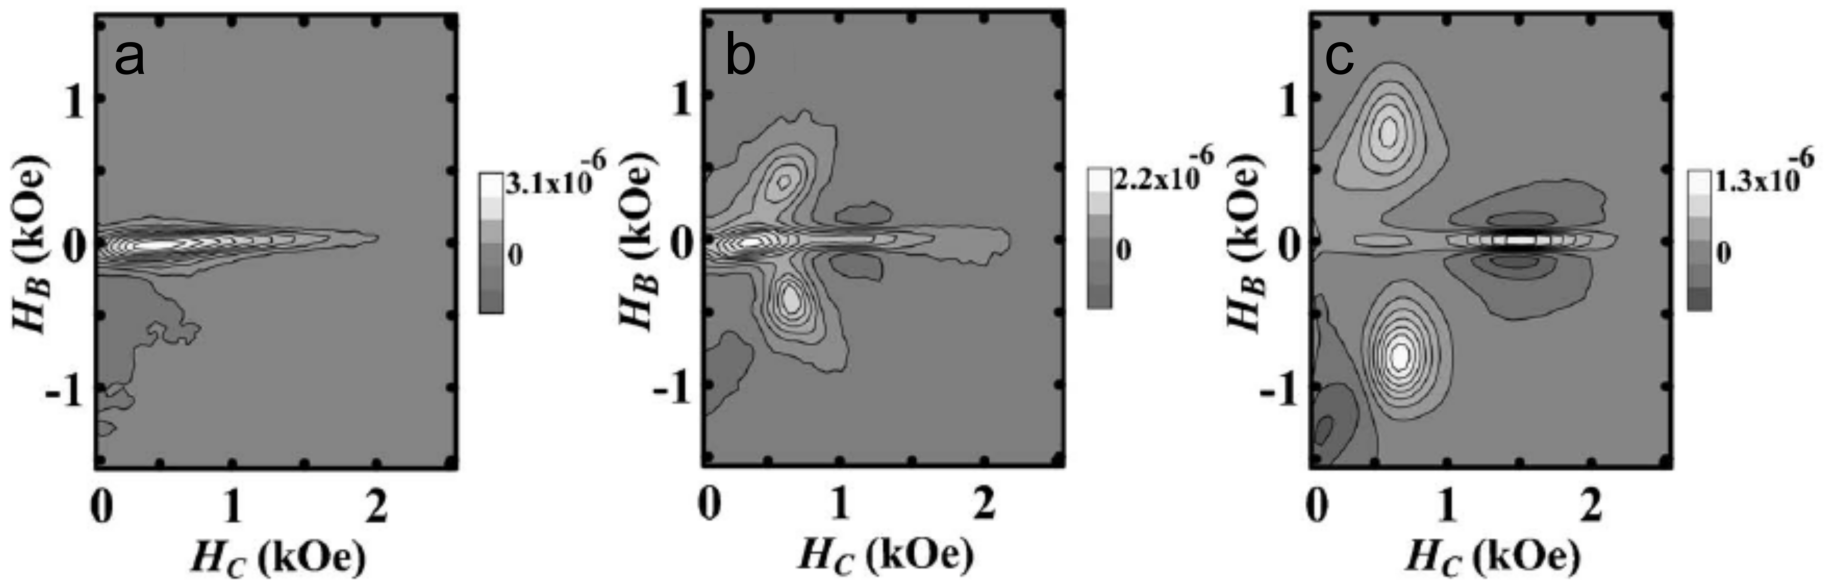
\includegraphics[width=\textwidth]{research-3/figs/Dumas2007_edit.pdf}
\caption[FORC diagram of a synthetic Fe dot array]{FORC diagrams for a weakly interacting 2D array of Fe dots fabricated using a nanoporous alumina shadow mask technique in conjuction with electron beam evaporation. a) The array with the smallest (52$\nm$) particles shows SD properties. b) The array with 58$\nm$ particles shows SD and PSD properties. c) The array with the largest particles (67$\nm$) shows purely PSD properties. (Reproduced from \citet{Dumas2007}, with permission from the author).}
\label{FIG_C4_Dumas2007}
\end{figure}\par

Fragmentation of the FORC diagram for non-uniformly magnetised particles has been observed in experimental studies \citep{Pike1999B,Dumas2007,Roberts2017,Zhao2017} (Fig. \ref{FIG_C4_Dumas2007})and in numerical models \citep{Carvallo2003,Roberts2017}; however, these studies did not include random field orientation distributions. The trend is, nevertheless, clear and is representative of the complex self-interactions brought about by nonuniform structures and multiple vortex nucleation/annihilation fields \citep{Pike1999B}. It is difficult to compare our results to the FORC signals measured by \citet{Muxworthy2006B} and \citet{Krasa2011} for synthetic patterned magnetite because many of their FORC diagrams appear to have smoothed the subtle features observed here, which raises questions about the integrity of these samples (e.g., crystallinity) or the adequateness of the FORC measurement density for these samples. However, a general trend is recognised in the elongation of the FORC diagram contours in the direction of a negative angle diagonal from the $B_u=0$ axis (Fig. \ref{FIG_C4_Muxworthy2006B}) probably related to region 5 in Fig. \ref{FIG_C4_07}. FORC diagrams for coarse-grained synthetic greigite samples by \citet{Roberts2011} also show this type of elongations as well as a negative ridge (Fig. \ref{FIG_C4_Roberts2011}i--l) probably caused by a fraction of SD particles.
\begin{figure}
\centering
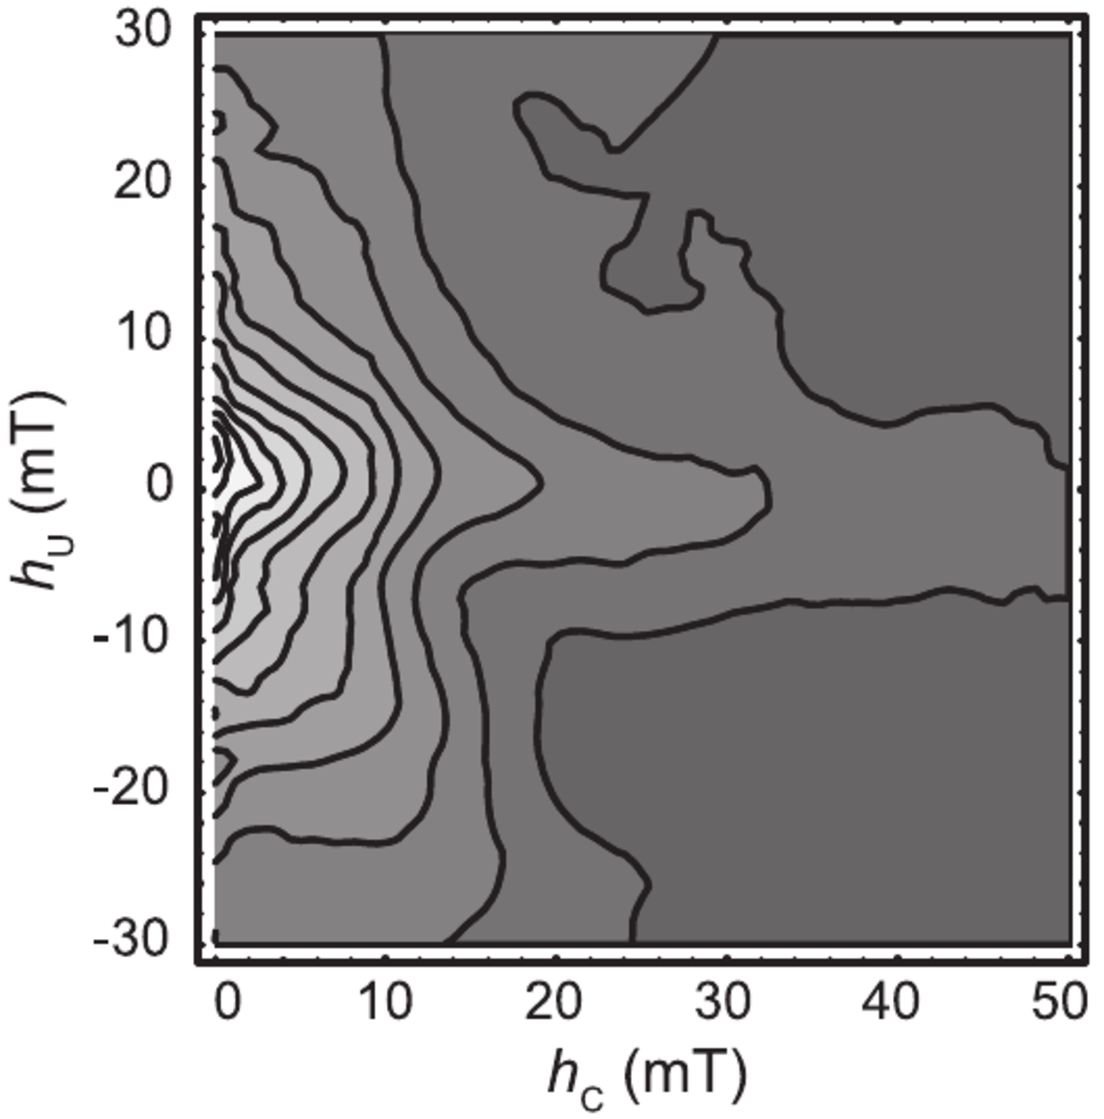
\includegraphics[width=0.4\textwidth]{research-3/figs/Muxworthy2006B.pdf}
\caption[FORC diagram of a synthetic magnetite 2D array]{FORC diagram (SF=4) for a weakly interacting 2D array of synthetic magnetite produced by electron beam lithography. Applied field along the elongation of the grains. (Reproduced from \citet{Muxworthy2006B}, with permission from the author).}
\label{FIG_C4_Muxworthy2006B}
\end{figure}\par

\citet{Pike1999B} obtained asymmetric nucleation and annihilation fields of magnetic vortices in nano-patterned Co dots; our models agree with this finding (Fig. \ref{FIG_C4_08}). However, \citet{Pike1999B} studied elongated disc-like particles where the vortex cores were always perpendicular to the particle plane that mostly underwent reversible motion from nucleation to annihilation as they traversed the particle. In this study, we demonstrate that different features on SV FORC diagrams are due to a variety of vortex nucleation and annihilation events, which depend on particle alignment with respect to the applied field and on the presence of distinctly different vortex states, i.e., the vortex energies and stabilities depend on their alignment within the crystalline structure \citep{ValdezGrijalva2017B}.
\begin{figure}
\centering
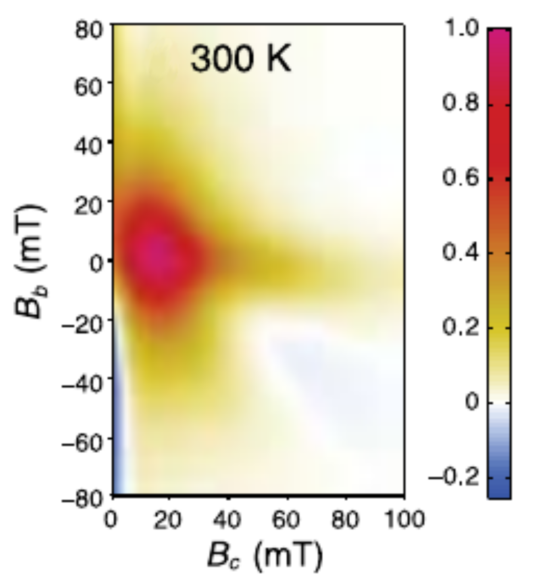
\includegraphics[width=0.4\textwidth]{research-3/figs/Roberts2011_edit.pdf}
\caption[FORC diagram of a synthetic coarse-grained greigite sample]{FORC diagram (SF=3) for a synthetic coarse-grained greigite sample of predominantly PSD particles. (Reproduced from \citet{Roberts2011}, with permission from the author).}
\label{FIG_C4_Roberts2011}
\end{figure}\par

FORC diagrams were averaged for simulations between 30 and 80$\nm$ (Fig. \ref{FIG_C4_09}a) and between 60 and 80$\nm$ (Fig. \ref{FIG_C4_09}b). That is, the particle size distributions are uniform (flat) for these averaged FORC diagrams. The FORC diagram in Fig. \ref{FIG_C4_09}a has a boomerang-shaped distribution surrounded by a variety of more complex responses. This pattern shows some similarities to the patterns observed by \citet{Dumas2007} for samples that included both SD and SV particles. The FORC distribution peak position coincides with the ensemble coercivity, while still having a response corresponding to the annihilation field of easy-aligned vortices.
\begin{figure}
\centering
\includegraphics[width=\textwidth]{research-3/figs/FIG_09.pdf}
\caption[Averaged-over-size FORC diagrams and raw hysteresis curves]{Averaged FORC diagrams (SF=4) (top) for multiple particle sizes and corresponding raw hysteresis curves (bottom). Uniform size distributions are used for particles a) $30\nm \leq d \leq 80\nm$ and b) $60\nm \leq d \leq 80\nm$. Dashed contour lines denote negative $\rho$ values.}
\label{FIG_C4_09}
\end{figure}\par

Both diagrams in Fig. \ref{FIG_C4_09} have a significant spread in the positive $B_u$ region. This effect is purely due to domain state, not magnetostatic interactions. The main peak for the averaged SV-dominant diagram (Fig. \ref{FIG_C4_09}b) occurs along the $B_u=0$ axis at $B_c\approx 52\mT$, which indicates a disconnect with the bulk coercivity of the ensemble ($B_\text{C}\approx 16\mT$). This is a departure from the usual interpretation of FORC diagrams, i.e., that the FORC diagram provides a map of the coercivity distribution. This interpretation holds for SD coherently rotating grains, where the peak response coincides with the value of the ensemble coercivity. It does not hold, however, for SV grains because their coercivity decreases with size while the position of the maximum moves toward higher $B_c$ values. Instead, for SV grains the FORC distribution peak, and most FORC features, should be interpreted as due to vortex nucleation/annihilation fields and their irreversible motions.\par
%-----------------------------------------------------

\section{Conclusion}
A micromagnetic FEM/BEM was employed to calculate FORC distributions for non-interacting ensembles of greigite across a size range that spans the SD to SV threshold. 500 random orientations from a uniform distribution over a sector of the unit sphere were used for each particle size. This choice was found to be in excellent agreement with previous calculations for SD greigite \citep{ValdezGrijalva2017}.\par

FORC diagrams are found to be extremely sensitive to the domain state of the simulated particles. When even a small fraction of particles starts to nucleate vortices, e.g., $d\approx$50$\nm$, this is reflected in the FORC diagram (Fig. \ref{FIG_C4_03}a compared to Fig. \ref{FIG_C4_02}). The same cannot be said of the Day plot (Fig. \ref{FIG_C4_05}a). Anomalous behaviour for particles sized 62 to 72$\nm$, with coercivity increasing with size was found; these particles plot in an unexpected region of the Day plot. The anomaly disappears for particles $>72\nm$, and when $d \geq 76\nm$ they have much lower $M_\text{RS}/M_\text{S}$ and higher $B_\text{CR}/B_\text{C}$ values.\par

Detailed FORC analysis and micromagnetic solutions for $d=80\nm$ particles reveals the meaning of the FORC diagram for SV ensembles as a map of vortex nucleation/annihilation fields. Interpretation of FORC diagrams as a coercivity distribution does not apply to SV systems (see \citet{Pike1999B,Roberts2017}). Recognition that the remanence in palaeomagnetic studies is often carried by vortex state particles should help users of FORC diagrams to avoid misinterpretation of vertical spread in FORC diagrams, just as it is recognised that vertical spread in MD particles is due to domain wall interactions within particles \citep{Pike2001}. For SD particles, the typical interpretation of the peak position coinciding with the coercivity of the sample holds; however, for SV-dominated samples, the position of the peak occurs at a value much higher than the bulk coercivity of the sample.\par
%-----------------------------------------------------
%\renewcommand\bibname{{References}}
%\bibliographystyle{elsarticle-harv}
%\bibliography{references}



%\chapter{First-order reversal curve diagram modelling of framboidal greigite}
\label{ch:res-4}
\fancyhead[L]{Chapter 5. FORC modelling of framboids}
\fancyhead[C]{}
\fancyhead[R]{}
\fancyfoot[C]{\thepage}

\section*{Abstract}
First-order reversal curve (FORC) diagrams are an increasingly used technique in rock magnetism that has the potential to identify magnetic domain state and magnetostatic inter-particle interactions. The hysteresis and FORC properties of non-interacting dispersions of greigite in the single-domain (SD) to single-vortex (SV) size range is well studied. However, most greigite occurs as highly interacting clusters. In this chapter, a micromagnetic method is used to study the FORC response of a simulated ensemble of highly interacting, close-packed greigite framboids. The magnetic signature of framboidal greigite is found to be very similar to that of multi-domain (MD) particles. Identification of MD-like FORC signals in samples known to contain greigite should be interpreted as produced by framboidal greigite.

\section{Introduction}
Greigite (Fe$_3$S$_4$) is a ferrimagnetic mineral often of authigenic origin in sediments \citep{Roberts2011}. It is most commonly found in strongly interacting, close-packed clusters called framboids \citep{Ariztegui1996,Rowan2006,Rowan2009,Roberts2011} (Fig. \ref{FIG_F00}).
\begin{figure}
\centering
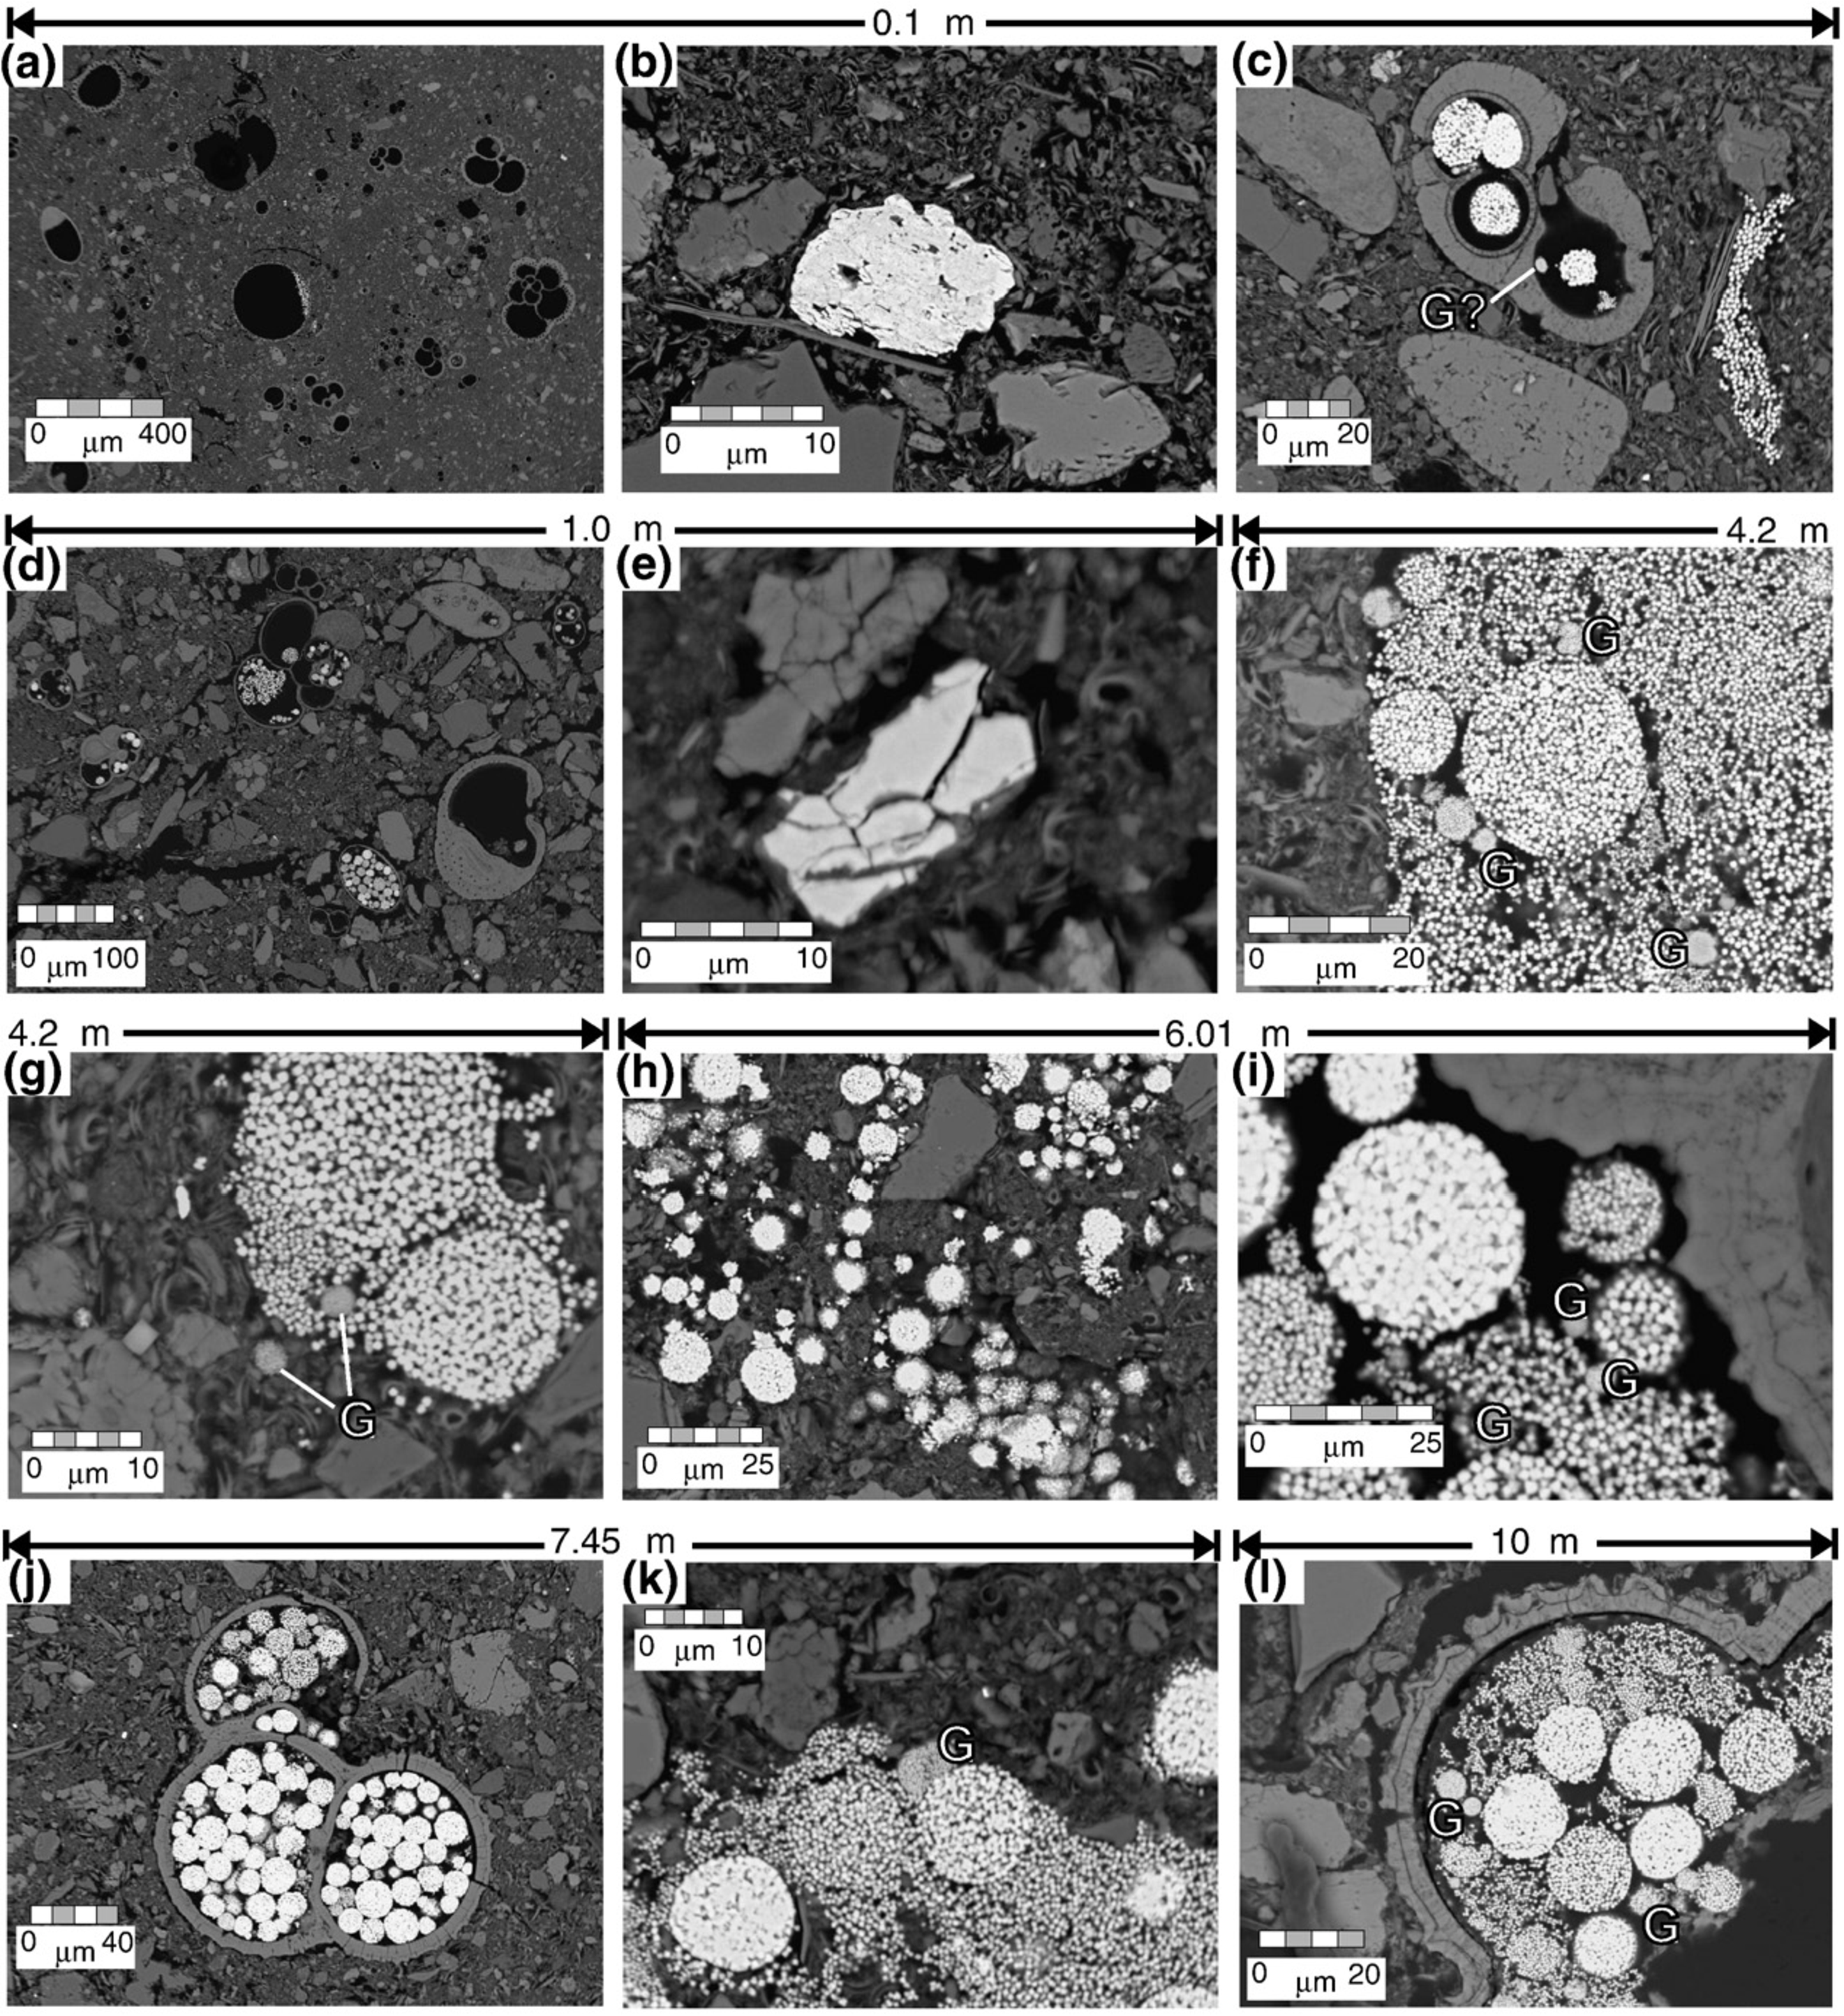
\includegraphics[width=0.5\textwidth]{research-4/figs/framboids_rowan.pdf}
\caption[SEM micrographs of framboidal greigite]{Scanning electron miscroscopy (SEM) micrographs of framboidal greigite (after \citet{Rowan2009}). Greigite grows authigenically in sediments as close-packed clusters (G), often in the presence of coarser-grained framboidal pyrite (FeS$_2$).}
\label{FIG_F00}
\end{figure}\par

The zero-field magnetic structure and stability properties of isolated greigite have been the subject of previous numerical studies (Chapter \ref{ch:res-1}; \citet{Muxworthy2013}). There have also been numerical simulations of the hysteresis and first-order reversal curve (FORC) properties of ideal single-domain (SD) grain (Chapter \ref{ch:res-2}) and single-vortex (SV) and SD grain (\ref{ch:res-3}) dispersions. However, the FORC properties of highly interacting ensembles of greigite is yet poorly understood.\par

In this chapter, a numerical micromagnetic finite element method (FEM) is employed to calculate the FORC response of a simulated ensemble of framboidal greigite composed of highly interacting, close-packed 30$\nm$ grains. At this size, these grains are SD in the non-interacing case (Chapter \ref{ch:res-3}) and produce FORC signals charactersitic of SD grains with cubic magnetocrystalline anisotropy (MCA) (Chapters \ref{ch:res-2},\ref{ch:res-3}).\par

Here, truncated-octahedral particles are chosen as the model geometry, because they are a common morphology for authigenic greigite \citep{Snowball1997,Roberts2011}. Also, truncated-octahedral solids can efficiently tessellate 3D space (the bitruncated cubic honeycomb) and thus produce the close-packed geometries observed in framboidal greigite.\par

Touching grains are theoretically problematic to model as possible exchange coupling between particles is not well understood. Here, a vanishing exchange coupling is assumed. Framboidal geometries with small gaps between the particles are used, so the only inter-particle interaction is magnetostatic.\par

Ferromagnetic materials have magnetisation states that are dependent on their magnetic (or thermal, chemical) history. This is the well-known phenomenon of magnetic hysteresis. Standard hysteresis measurements proceed by saturating the magnetisation by applying a saturating magnetic field $\boldsymbol{B}$ ($=\mu_0\boldsymbol{H}$) with strength $B_{\text{sat}}$; in this saturated state, magnetisations are uniform and completely aligned with the applied field. Gradually, the magnetic field strength is decreased to desaturate the magnetic material. A curve $M=M(B)$ of the projection of the material's magnetisation on the applied field direction $M=\boldsymbol{M}\cdot\boldsymbol{\hat{n}}$ (where $\boldsymbol{\hat{n}}$ is a unit vector in the direction of the applied field) against the applied field strength $B$ is traced. When the applied field is removed, the remanent magnetisation state is left. The ratio of the saturation remanent state magnetisation $M_{\text{RS}} \geq 0$ to the saturation magnetisation $M_{\text{S}}$ is one of the key magnetic hysteresis parameters \citep{Dunlop}. The applied magnetic field strength is then increased in the direction opposite the initial (effectively, making $B<0$): the applied field value at which a magnetisation $M=0$ state is obtained is called the coercivity, $B_\text{C}$. If from this state the field is taken back to zero, a magnetisation $M>0$ is obtained; however, there exists a field value $B_{\text{CR}}<B_{\text{C}}$, called the coercivity of remanence, from which a remanent $M=0$ state is obtained for $B=0$. These fields and the ratio $B_{\text{CR}}/B_{\text{C}}$ are key parameters characterising a hysteresis curve. To complete a hysteresis loop, the magnetisation is driven to a negatively saturated state and gradually returned to the initial positive saturation state. This traces the main (upper and lower) branches of a hysteresis loop.\par

A scatter plot of the ratio $M_{\text{RS}}/M_{\text{S}}$ against $B_{\text{CR}}/B_{\text{C}}$ is called a Day plot \citep{Day1977} and is one of the most common plots in rock magnetism \citep{Dunlop}. Although these basic magnetic hysteresis parameters can be useful to discern the magnetic domain state and magnetisation reversal mechanisms of magnetic systems, it has been argued recently that the Day plot can lead to erroneous interpretations \citep{Egli2014,Roberts2017}. It is logical that access to the interior of the hysteresis loop can reveal more information about magnetic behaviours, which is the basic idea behind the calculation of $B_{\text{CR}}$.\par

\section{Methodology}
\subsection{The micromagnetic method}
A ferromagnetic (in the broad sense, i.e., including ferrimagnetic behaviour) material has a Gibbs free-energy functional (excluding the effects of thermal fluctuations and magnetostriction) which can be written as \citep{Brown}:
\begin{equation}
E_\text{G} = \int_{\Omega} (\phi_{\text{exchange}} + \phi_{\text{anisotropy}} + \phi_{\text{stray}} + \phi_{\text{external}})\,\text{d}^3 \boldsymbol{r},
\end{equation}
where $\Omega$ is the ferromagnetic volume and $\text{d}^3 \boldsymbol{r}$ the volume differential, so integration is carried out over the ferromagnetic body. Here,
\begin{equation}
\phi_{\text{exchange}}=A|\nabla\boldsymbol{m}|^2,
\end{equation}
where $\boldsymbol{m}$ is the reduced (unitary) magnetisation vector and $A$ the exchange stiffness constant, is an expression providing a continuum approximation of the energy density due to quantum-mechanical exchange forces between atomic spins \citep{Landau1935}.
\begin{equation}
\phi_{\text{anisotropy}}=\frac{K_1}{2}\sum_{i\neq j}\gamma_i^2\gamma_j^2 + K_2\prod_i\gamma_i^2,
\end{equation}
where $\gamma_i$ denote the direction cosines and $K_1,K_2$ the first and second magnetocrystalline (MCA) anisotropy constants, respectively, is the MCA energy density for cubic-anisotropic ferromagnets. In terms of the reduced magnetisation vector components this has the form:
\begin{equation}
\phi_{\text{anisotropy}}=K_1(m_x^2m_y^2+m_y^2m_z^2+m_z^2m_x^2),
\end{equation}
where $K_2$ has been neglected since in the cubic anisotropy system we are assuming, $K_1$ is the dominant term at room temperature. The magnetic Gibbs free-energy associated with the magnetostatic self-interaction of the ferromagnetic body and the stray magnetic field $\boldsymbol{H}_{\text{stray}}$ it produces is given by \citep{Brown}:
\begin{equation}
\phi_{\text{stray}}=-\frac{\mu_0M_\text{S}}{2} \boldsymbol{m} \cdot \boldsymbol{H}_{\text{stray}}
\end{equation}
where $M_\text{S}$ is the saturation magnetisation and $\mu_0=4\pi \times 10^{{-}7}\,\text{T}\text{m}/\text{A}$ is the magnetic constant or vacuum permeability. Finally, the energy density due to the magnetostatic interaction of the ferromagnetic body and an external field $\boldsymbol{H}_{\text{external}}$ is:
\begin{equation}
\phi_{\text{external}}=-\mu_0 M_{\text{S}} \boldsymbol{m} \cdot \boldsymbol{H}_{\text{external}}.
\end{equation}

From thermodynamics, it is well known that under isothermal and isobaric conditions a system will be driven spontanteously toward an equilibrium state with locally minimal Gibbs free-energy. Micromagnetic algorithms aim to find the equilibrium magnetisation $\boldsymbol{m}$ by minimising the Gibbs free-energy functional \citep{Fischbacher2017}. Here, a modified gradient-descent method \citep{OConbhui2017} is used.\par

Numerical solutions require a discretisation of the spatial domain into a grid or mesh with a finite number of points on which numerical solutions are calculated. In FEMs, three-dimensional space is decomposed into tetrahedral pieces called finite elements with the vertices of these elements called the nodes. On each of the mesh nodes, a unit vector is initially defined to create an initial guess; the micromagnetic algorithm then attempts to minimise the magnetic Gibbs free-energy by variating the orientation of each of these vectors while ensuring they remain unitary. In micromagnetic theory \citep{Brown} there are some linearisations, which means that there should not be large variations in the direction of $\boldsymbol{m}$ between neigbouring nodes. For unconstrained micromagnetic models it is expected that the microstructure will contain nouniform structures at least to some degree. To model nonuniform structures it is sufficient that the spatial discretisation in the model is always smaller than the exchange length $l_\text{exch} = \sqrt{2A/\mu_0M_\text{S}^2}$ \citep{Rave1998}, which for greigite is $l_\text{exch} \approx 6.6\, \text{nm}$; a maximum element size of 5$\nm$ has been chosen for all the meshes. The non-local problem of calculating the stray field is handled via a hybrid finite-element/boundary-element formulation \citep{Fredkin1990}.\par

\subsection{The FORC model}
First-order reversal curves are a set of partial hysteresis curves obtained from magnetisation states on the upper branch of the hysteresis loop for different field values $B_a$ \citep{Mayergoyz1986}. For a given $B_a$ and $M(B_a)$, the field $B=B_b$ is increased to positive saturation to trace a magnetisation curve. This proceedure for a number of $B_a$ values creates a magnetisation function on two variables $M=M(B_a,B_b)$ for $B_b \geq B_a$. The FORC distribution $\rho$ is then defined as \citep{Roberts2000}:
\begin{equation}\label{forc distribution}
\rho = -\frac{\mu_0^2}{2}\frac{\partial^2 M}{\partial B_a \partial B_b}.
\end{equation}\par

It has been argued that, the FORC distribution is an empirical analog of the Preisach distribution which is well defined for magnetic systems that do not necessarily obey the strict conditions imposed by the Preisach model \citep{Mayergoyz1986}. Contour plots of the FORC distribution are called FORC diagrams and have been used increasingly as a proxy for the magnetic domain state and magnetic reversal behaviour of a variety of systems \citep{Pike1999,Pike2001,Roberts2000,Dumas2007,Egli2010,Egli2014,Biasi2016,Proenca2017,Zhao2017}.\par

Calculation of the FORC distribution (Eq. \ref{forc distribution}) is performed by least-squares fitting of a second degree polynomial surface $M(B_a,B_b)=a_0 + a_1 B_a + a_2 B_b + a_3 B_a B_b + a_4 B_a^2 + a_5 B_b^2 + e$, where $e$ is a collection of error terms, on a subgrid of the magnetisation function $M(B_a,B_b)$ including ($2\times\text{SF}+1$)$^2$ points in the vicinity of $(B_a, B_b)$ as determined by the smoothing factor SF \citep{Pike1999}. If the magnetisation is approximated in this manner, calculation of Eq. \ref{forc distribution} yields $\rho=-\mu_0^2 a_3 / 2$. Rotated $(B_b,\,B_a)$ axes, the so-called coercive field $B_c = (B_b - B_a)/2$ (not to be confused with the coercivity $B_\text{C}$) and interaction field $B_u = (B_a + B_b)/2$, respectively, are used for contour plots to produce FORC diagrams.\par

In an ensemble of randomly oriented particles, there are equal probabilities of finding particles with any orientation within an area element of the unit sphere. To simulate a randomly oriented dispersion of identical particles efficiently, it is necessary to obtain a number of applied field directions (equivalently, particle orientations with respect to the applied field) each of them representative of a given area on the unit sphere. Additionally all these areas should span the unit sphere or alternatively, in high symmetry particle scenarios, a section of the sphere which can recreate the particle geometry under rotation operations (Chapters \ref{ch:res-2}, \ref{ch:res-3}). Given the symmetry of the modelled framboidal cluster geometries (Fig. \ref{FIG_F01}) it is sufficient to simulate the effects of field orientations on the spherical triangle delimited by $(1, 0, 0), (a, a, a), (0, 0, 1)$, where $a=1/\sqrt{3}$. Then, the spherical triangle is subdivided into roughly equiareal triangle sub-units to obtain 85 triangular cells. Each cell represents a field orientation we obtain the FORC response for here, with the coordinates of the centre of the cell used as the direction of the field. The weighted average (using the cell area as the weight for each field direction) of all the FORC responses for each of these field orientations is the approximation to the total FORC response of the ensemble:
\begin{equation}
M(B_b, B_a)_{\text{total}} = \frac{\sum_i^{\text{cells}}M_i(B_b,B_a) A_i}{\sum_i^{\text{cells}}A_i},
\end{equation}
where $A_i$ is the area of cell $i$ and $M_i$ the FORC response of the framboid for field direction associated with cell $i$.
\begin{figure}
\centering
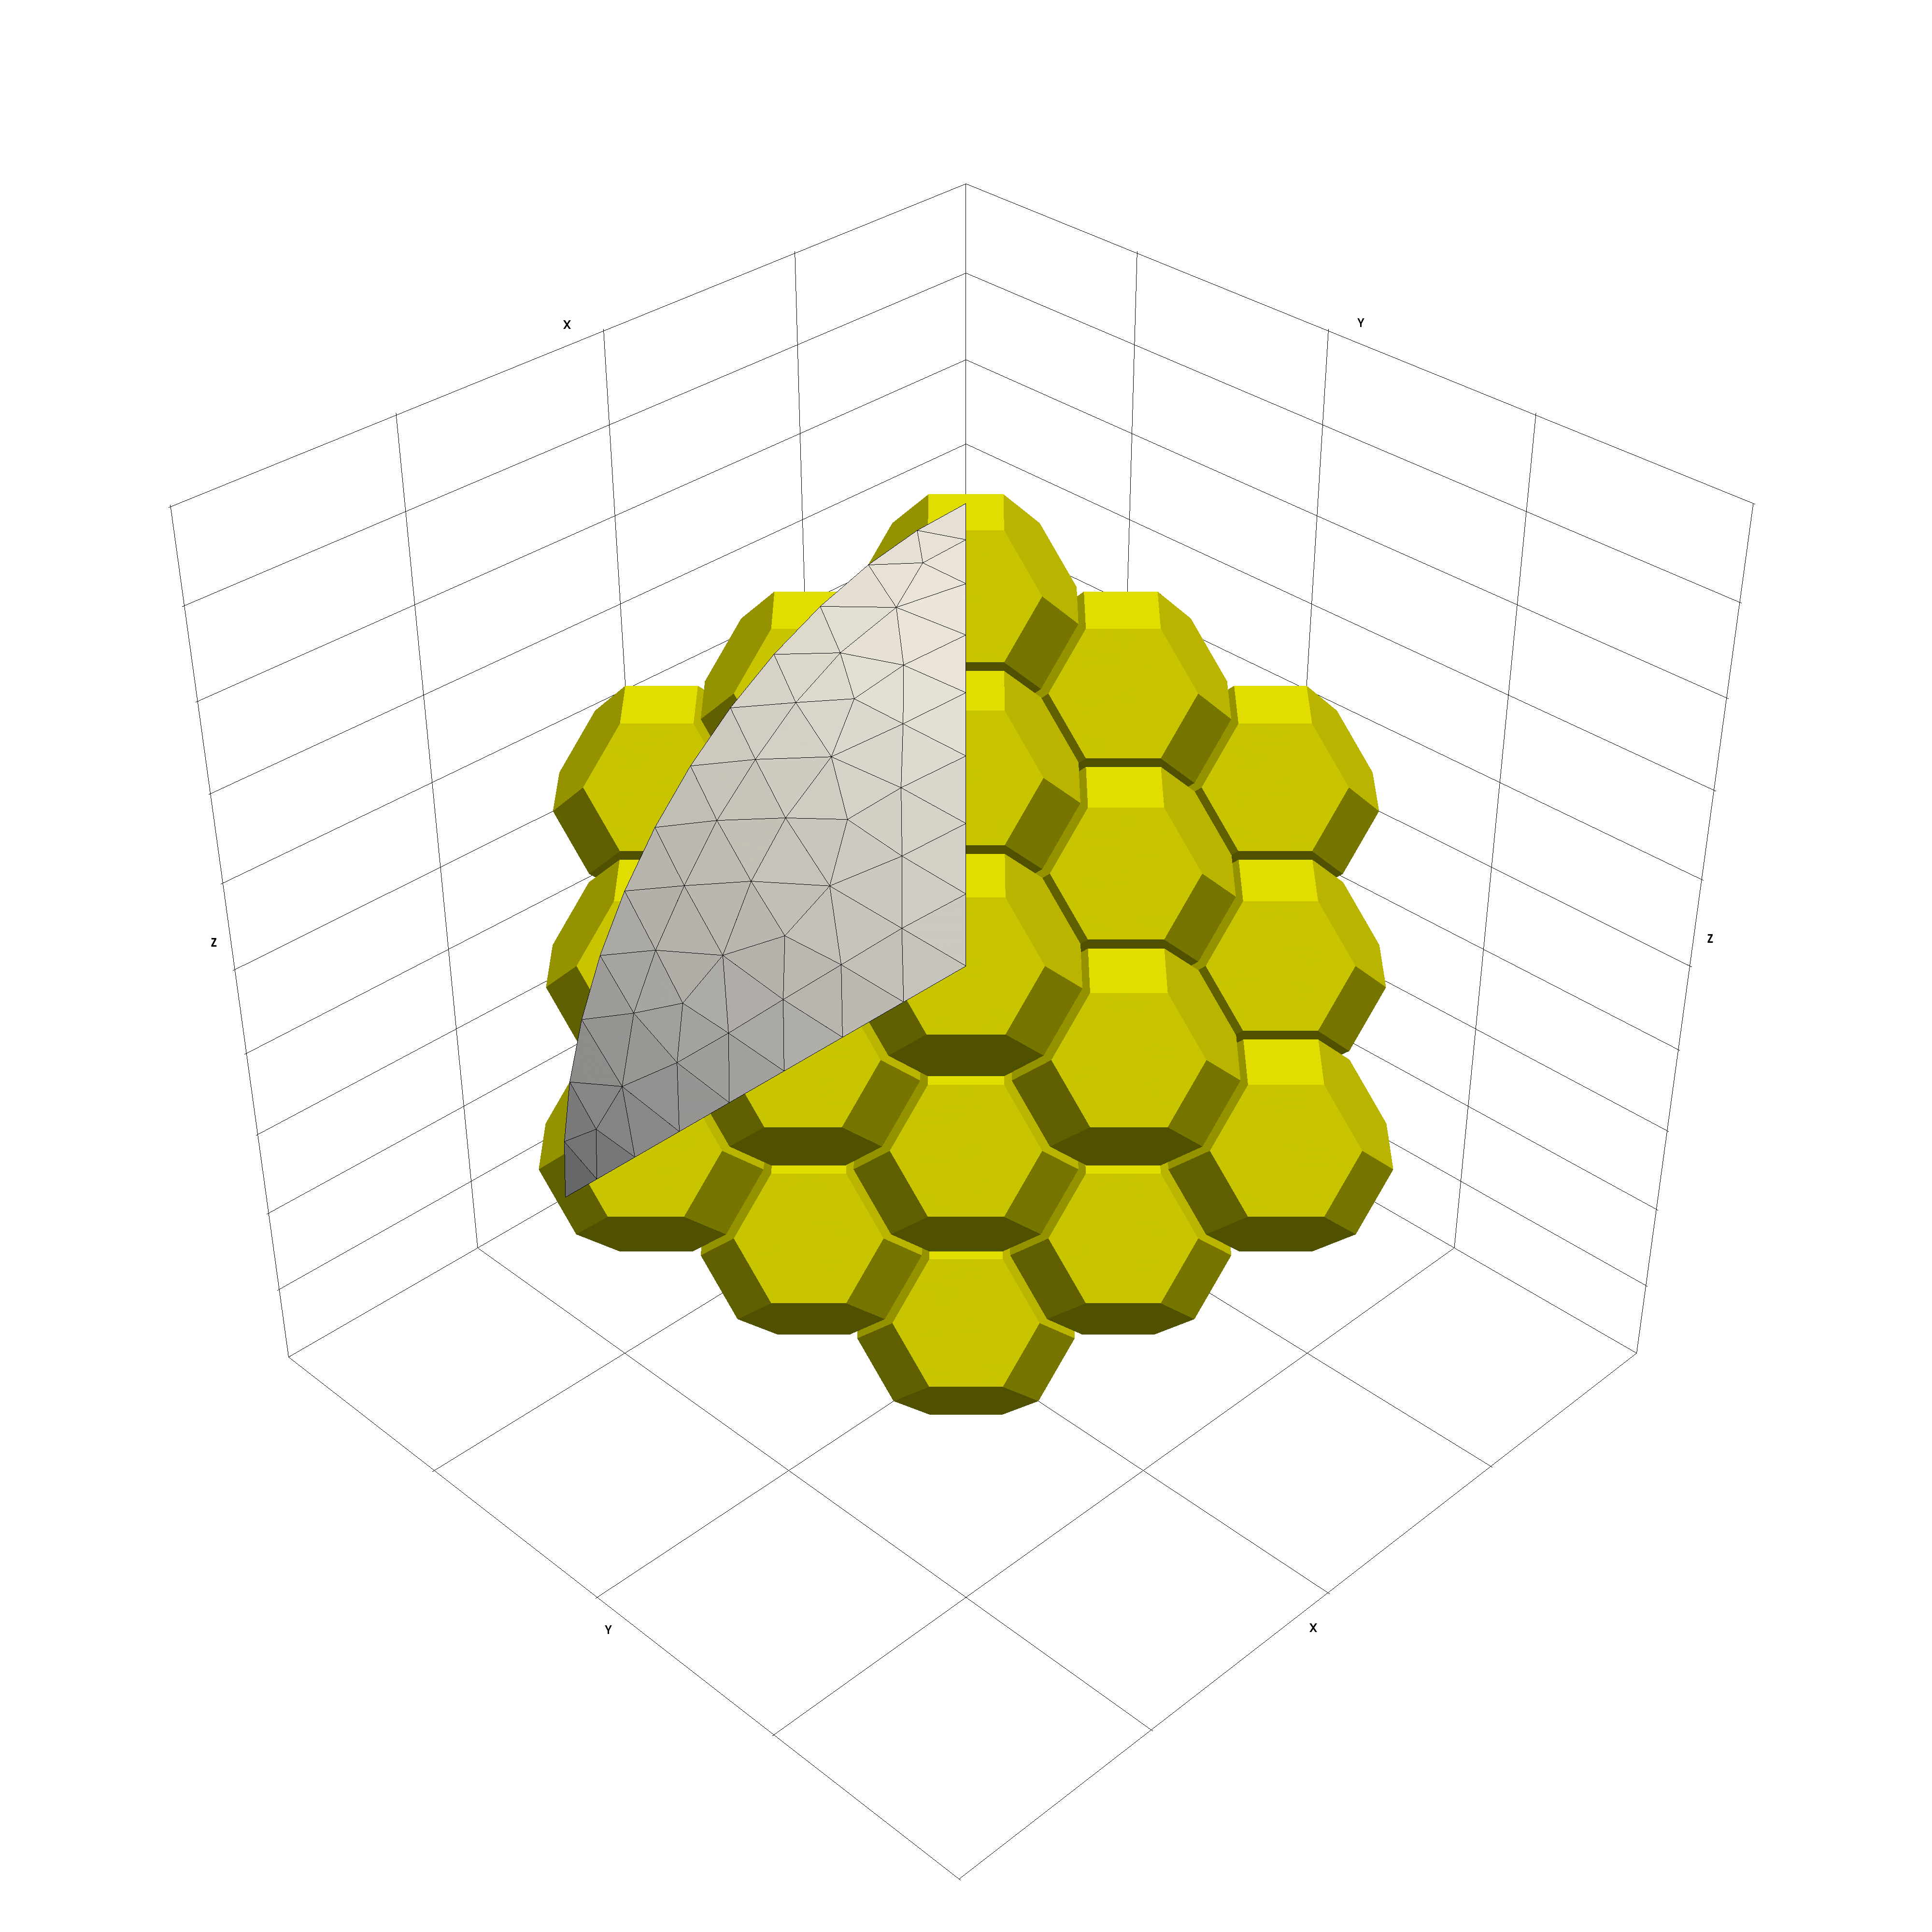
\includegraphics[width=0.6\textwidth]{research-4/figs/mesh_orientations_HD.png}
\caption[Framboidal mesh and field orientations]{Framboidal mesh and field orientations. Field orientations are obtained from a triangular mesh over the spherical triangle delimited by $(1, 0, 0), (a, a, a), (0, 0, 1)$, where $a=1/\sqrt{3}$. Given the symmetry of the cluster, this region contains all field orientations of interest. The framboid contains 65 truncated octahedral particles each with size $d=30\nm$. The small gap between the particles is $\roughly$2$\nm$.}
\label{FIG_F01}
\end{figure}\par

Since these calculations are computationally intensive, it is important to reduce further the amount of calculations. For each field orientation, the upper branch of the hysteresis loop is calculated. Most of the curve is traced by the sum of reversible motions of the magnetisations in each of the individual particles in the framboid. Therefore, FORCs need only to be calculated for $B_a$ field values for which at least one particle undergoes an irreversible rotation (switching) (Chapters \ref{ch:res-2}, \ref{ch:res-3}).\par

A saturating field $B_{\text{sat}}=250\mT$ and an external field rate of change of 2$\mT$ is used for all calculations. This means that for each field orientation we calculate 251 FORCs to obtain the FORC signal of a given cluster orientation.\par

\section{Results}
\subsection{The hysteresis and FORC response of framboidal greigite}\label{framFORC}
The FORC response is dependent on field orientation with respect to the framboid; all the 30$\nm$ particles have the same orientation. When the field is close to the isolated particle easy axis $<$111$>$, the hysteresis response of the framboid is saturated as low as $\roughly 50\mT$ (Fig. \ref{FIG_F02}a). Complex local interaction fields cause outer particles to coherently rotate to minimise the stray fields as the field is decreased. The remanent state is a double magnetic super-vortex with a low remanence $\roughly 0.1 \, M_\text{S}$ that is due to the effective magnetic flux-closure brought about by the super-vortex \citep{Harrison2002,Evans2006} structures (Fig. \ref{FIG_Frem}). All particles in the framboid remain in a SD state throughout the hysteresis and FORCs.
\begin{figure}
\centering
\includegraphics[width=\textwidth]{research-4/figs/forcs_easy_hard.pdf}
\caption[FORCs for fields along an easy and a hard axis]{FORCs for greigite clusters with 30$\nm$ crystallites for fields along an easy (a, b) and a hard (c, d) axis. When the field is aligned close to an easy axis, there is a peak FORC response on the $B_u=0$ axis at $B_c\approx 80\mT$ (b). For fields close to the hard axis, the FORC response has a peak for $B_c\approx 10\mT$ (d).}
\label{FIG_F02}
\end{figure}
\par

The FORC diagram for the easy axis-aligned applied field (Fig. \ref{FIG_F02}b) has a positive peak at $B_c\approx 80\mT$ roughly 5$\mT$ above the $B_u=0$ axis. A negative response of comparable magnitude is situated below and to the left of the distribution peak. The positive peak response corresponds to the large upward jumps experienced by the reversal curve starting at the lowest switching field $B_a\approx{-}80\mT$ as it approaches positive saturation (Fig. \ref{FIG_F02}a). The negative response is caused by irreversible switching of individual particles in the framboid on FORCs with higher $B_a$ values at $B_b\approx 75 \mT$. Most of the FORC diagram has a noisy appearance due to the complexity of individual particle responses caused by the local interaction fields. However, a large, continuous, positive response close to the $B_c=0$ axis is important as it was found for all field orientations.
\begin{figure}
\centering
\includegraphics[width=\textwidth]{research-4/figs/remanent_supervortex.pdf}
\caption[Framboid remanent super-vortex states]{Framboid remanent super-vortex states. Super-vortex structures are the remanent state for all field orientations. Shown here: (a) field close to an easy axis; (b) field close to a hard axis; (c) field close to a saddle point; (d) field close to an intermediate direction between the easy, hard and saddle point directions. The net magnetic moment of the ensemble is $\roughly 12^{\circ}$ from the applied field.}
\label{FIG_Frem}
\end{figure}\par

When the applied field is close to a hard axis, the hysteresis and FORC response is very different. The hysteresis main branches are much more rounded, desaturating via reversible motion and experiencing the first irreversible switchings at roughly 150$\mT$ (Fig. \ref{FIG_F02}c) which are much smaller than the jumps for the easy axis-aligned applied field response (Fig. \ref{FIG_F02}a). The FORC diagram (Fig. \ref{FIG_F02}d) is dominated by signals close to the $B_c=0$ axis.\par

Averaging the response for all 85 field orientations results in a very smooth set of FORCs (Fig. \ref{FIG_F03}a). The remanence of the framboid ensemble is $M_\text{RS}/M_\text{S}\approx 0.1$ and the hysteretic coercivity $B_\text{C}\approx 5\mT$; compare this to the remanence and coercivity of a noninteracting ensemble of isolated SD greigite particles of the same size, $M_\text{RS}/M_\text{S}\approx 0.86$ and $B_\text{C}\approx 24\mT$, respectively (Chapter \ref{ch:res-3}). The magnetostatic interactions between the particles in the framboids cause large decreases in the remanence and coercivity. The saturating field for the framboid ensemble is roughly 150$\mT$.
\begin{figure}
\centering
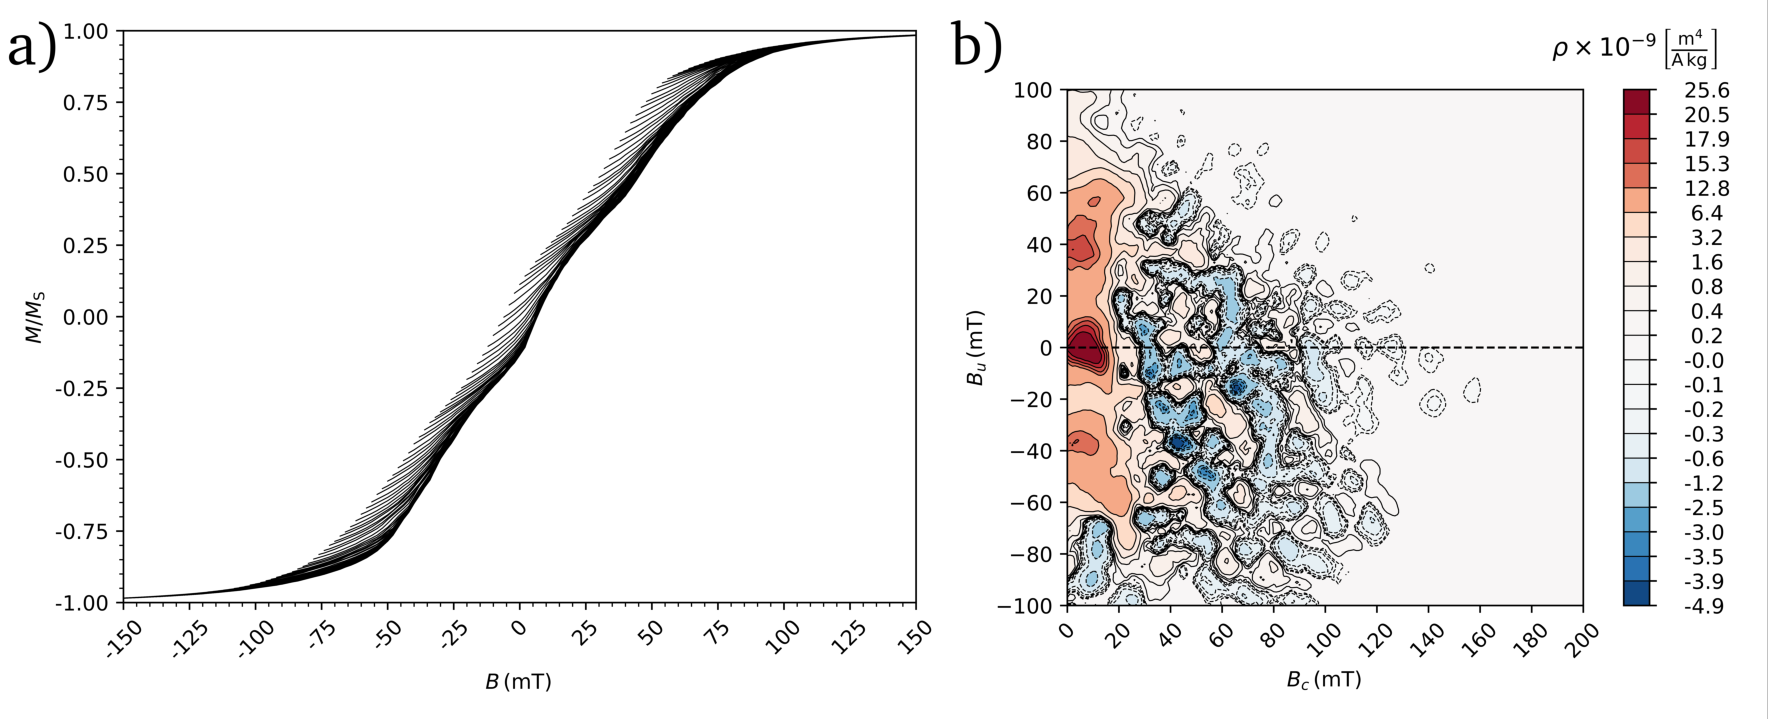
\includegraphics[width=\textwidth]{research-4/figs/forc_avg.pdf}
\caption[FORCs of the framboid dispersion]{FORCs of the greigite framboid dispersion. The framboids are formed by 65 particles identically aligned and with equal size $d=$30$\nm$. Averaging over the 85 field directions, the raw hysteresis/FORCs are smooth (a). The FORC response (b) is MD-like.}
\label{FIG_F03}
\end{figure}
\par

The FORC diagram of the simulated ensemble of framboidal clusters (Fig. \ref{FIG_F03}b) is dominated by a large response roughly centered at ($B_c=10\mT,B_u=0$) and two lobes roughly at ($B_c=10\mT,B_u=\pm 40\mT$). These sources are part of a larger, continuous signal roughly in the rectangle defined by coordinates ($B_c=0,B_u={-}60\mT$), ($B_c=20\mT,B_u={-}60\mT$), ($B_c=20\mT,B_u=100\mT$), ($B_c=0,B_u=100\mT$). This is because the set of averaged FORCs are very smooth and do not experience sharp discontinuities on the path tho positive saturation; therefore, the signal is dominated by the differences in magnetisation values along the upper branch that serve as starting points for the FORCs.\par

The negative and smaller positive responses form a noisy region to the right of this rectangle. However, these are only $\roughly 20 {\%}$ the magnitude of the peak response at maximum on some very small regions, and most of it is less than $\roughly 10 {\%}$. The simulated FORC response of an ensemble of randomly aligned greigite framboids (composed of 30$\nm$ particles) is much lower per mass than the response of noninteracting, isolated 30$\nm$ grains: 25.6$\times 10^{{-}9}\,\text{m}^4\text{A}^{{-}1}\text{kg}^{{-}1}$ and 531.6$\times 10^{{-}9}\,\text{m}^4\text{A}^{{-}1}\text{kg}^{{-}1}$ (Chapter \ref{ch:res-3}) for the peak responses, respectively.\par

Using the model of Chapter \ref{ch:res-3}, the FORC response of noninteracting ensembles of isolated greigite particles in the size range 30--80$\nm$ is obtained to produce FORC diagrams of mixtures of framboidal greigite and isolated particles in the SD and SV magnetic domain states. FORC diagrams of mixtures of equal mass framboidal and noninteracting SD particles (30--48$\nm$) (Fig. \ref{FIG_F04}a) and equal mass framboidal and noninteracting SV particles (70--80$\nm$) (Fig. \ref{FIG_F04}b) are presented.\par

The mixture of framboidal greigite and noninteracting SD particles (Fig. \ref{FIG_F04}a) is dominated by the noninteracting SD signal, erasing most of the noisy structure while keeping the important framboidal source close to the $B_c=0$ axis. When noninteracting SV particles are included (Fig. \ref{FIG_F04}b) to the framboid signal, the response is dominated by the SV particles. As with the mixture of SD and framboidal greigite, most of the noisy region disappears on account of it being so faint and there is more behaviour in the region close to the $B_c=0$ axis as SV particles' response is also in this region (Chapter \ref{ch:res-3}).
\begin{figure}
\centering
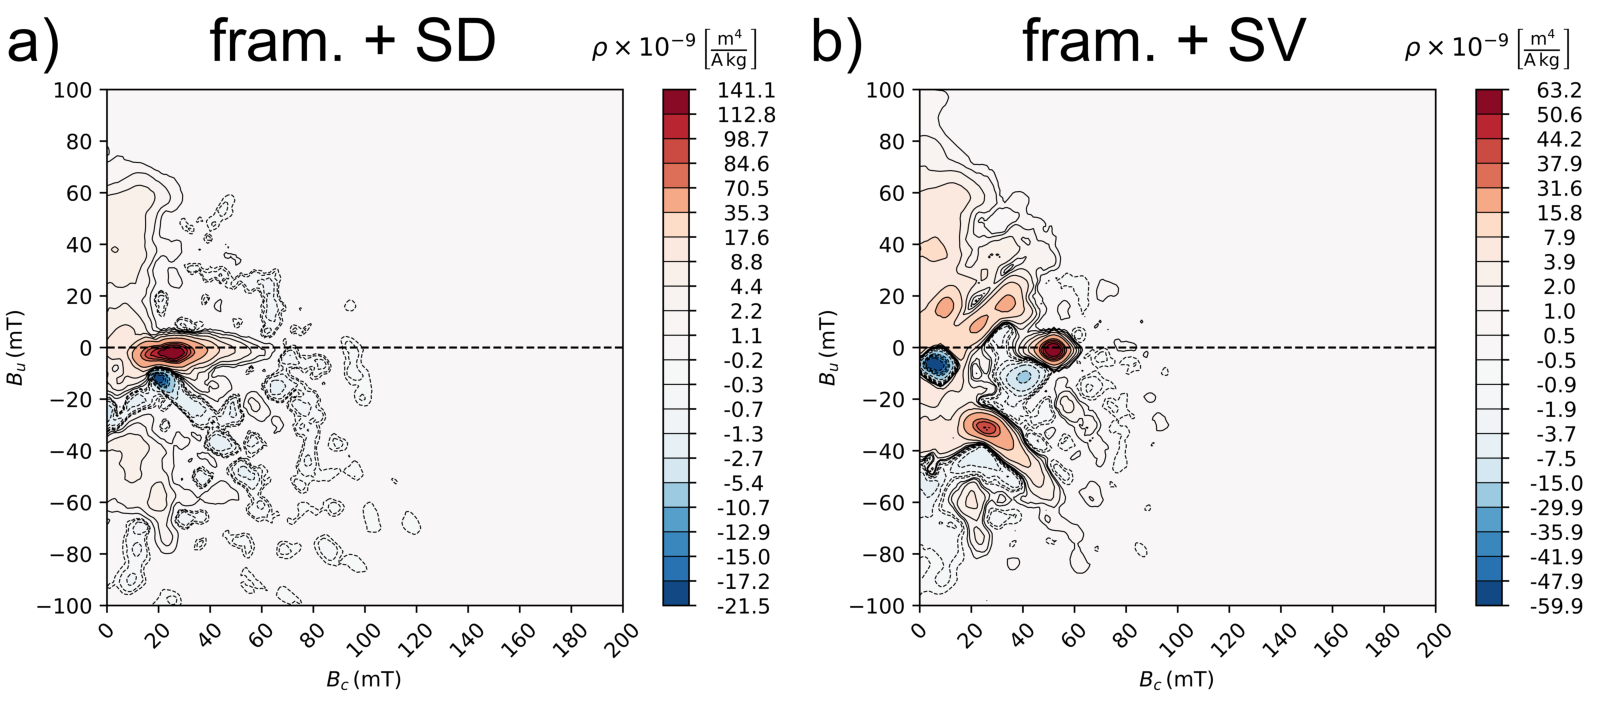
\includegraphics[width=\textwidth]{research-4/figs/forc_mix.pdf}
\caption[FORCs of a dispersion of framboids and non-interacting particles]{FORCs of a dispersion of equal-mass framboids and non-interacting SD (a) and SV (b) particles. The signal is dominated by the non-interacting particles because the framboid signal is weaker per unit mass. The framboid signal is still visible, however, as it occupies regions the non-interacting particles do not.}
\label{FIG_F04}
\end{figure}
\par

A scatter plot of the remanence of saturation $M_\text{RS}/M_\text{S}$ against the coercivity of remanence $B_\text{CR}$ to coercivity $B_\text{C}$ ratio, (Day plot \citep{Day1977}), reveals the simulated ensemble of framboidal greigite in a region that is unoccupied by the noninteracting, isolated particles (Fig. \ref{FIG_F05}), i.e., a region with a remanence as low as that of ensembles of SV particles $\roughly 80\nm$ but $B_\text{CR}/B_\text{C}$ values that are expected of smaller particles $\roughly 70\nm$ (Chapter \ref{ch:res-3}). Increasing content of SD or SV noninteracting particles have very different effects on the Day plot (Fig. \ref{FIG_F05}): increasing the SD content increases the remanence and decreases the $B_\text{CR}/B_\text{C}$ ratio; whereas, increasing the SV content has little effect on the remanence while increasing the $B_\text{CR}/B_\text{C}$ value.\par
\begin{figure}
\centering
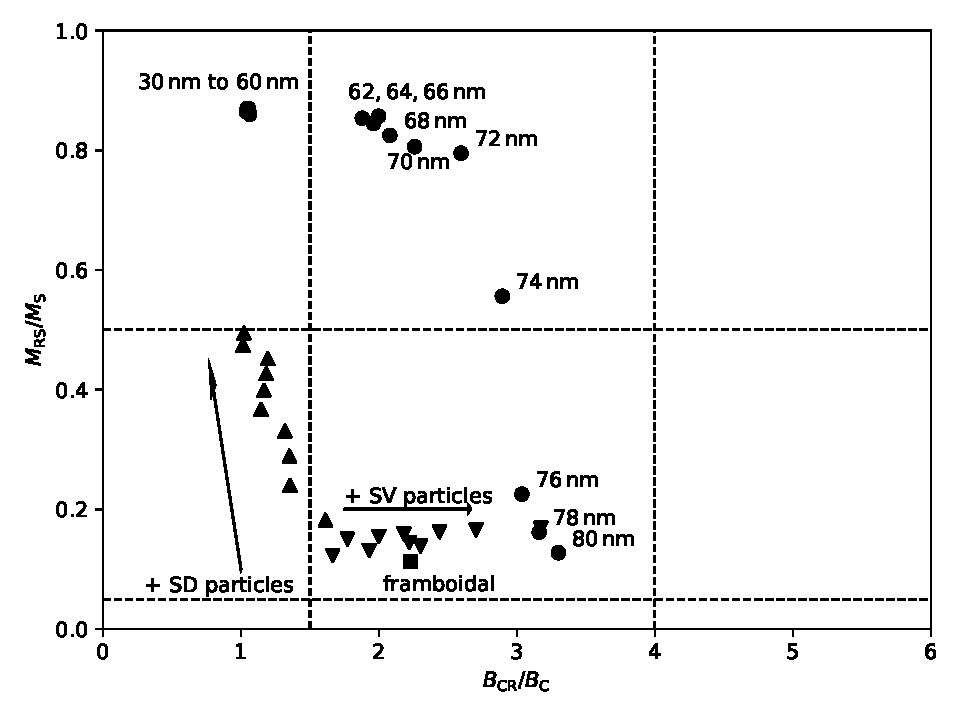
\includegraphics[width=0.8\textwidth]{research-4/figs/DayPlot.pdf}
\caption[Day plot of framboid and noninteraring particles mixtures]{Day plot of framboid and noninteraring particles mixtures. The framboidal clusters (square) plots in a region with very low $M_\text{RS}/M_\text{S}\approx 0.1$ and $B_\text{CR}/B_\text{C}\approx 2.2$. Increasing non-interacting SD particles content increases $M_\text{RS}/M_\text{S}$ and reduces $B_\text{CR}/B_\text{C}$. With increasing non-interacting SV particles content, the effect is to increase $B_\text{CR}/B_\text{C}$.}
\label{FIG_F05}
\end{figure}
\par

\subsection{Hysteresis of larger particle framboids}
An attempt was made to investigate FORC diagrams for assemblages of particles which are SV when isolated, however, due to memory and time constraints, the FORC response of larger particle framboids could not simulated. Instead, to investigate this, hysteresis simulations of framboids composed of fifteen (compared to 65 particles in Section \ref{framFORC}), larger SV particles with size $d=76\nm$ particles were carried out for a few selected field orientations. When the applied field is close to the easy axis the main branches remain saturated down to 50$\mT$ (Fig. \ref{FIG_F06}). As the field is decreased below this value, outer particles in the framboid nucleate hard-aligned vortices (Fig. \ref{FIG_F06}a). The remanent state (Fig. \ref{FIG_F06}b) has a super-vortex structure in which most particles are individually in a two-domain state with very clearly defined domain walls (Fig. \ref{FIG_F06}b, green). This state is remarkably similar to the easy-aligned SV state exhibited by large $>$200$\nm$ particles (Chapter \ref{ch:res-1}) with six easy aligned domains curling around the vortex core. However, in this super-vortex structure, outer particles are in a two-domain state and the six easy aligned magnetic domains span multiple particles. Non-interacting 76$\nm$ particles nucleate vortices (Chapter \ref{ch:res-3}); however, for this field orientation, the innermost particle in the cluster always remains in a SD state due to the internal magnetostatic interactions (Fig. \ref{FIG_F06}b, grey line). This is likely true for larger assemblages as the interaction fields deep inside the framboids will be stronger, thus favouring SD configurations for larger fractions of the crystallites in the framboid. This means that, for larger framboids composed of larger crystallites, the FORC signal could be very similar to the signal of framboids composed of SD crystallites (Section \ref{framFORC}).
\begin{figure}
\centering
\includegraphics[width=0.9\textwidth]{research-4/figs/loop21_76nm_annotated.pdf}
\caption[Hysteresis of a framboid with 76$\nm$ particles]{Hysteresis of a framboid with 76$\nm$ particlesfor a field aligned closely with the easy axis. The magnetisation remains saturated down to $\roughly$50$\mT$ when a few particles nucleate vortices (a). The remanent state is a super-vortex structure (b) with most of the particles in a two-domain state. Domain walls are visible as thin, green regions. The net magnetic moment of the innermost particle (grey line) is always close to one as it remains in a SD sate throughout hysteresis.}
\label{FIG_F06}
\end{figure}
\par

\section{Discussion}
The FORC response of a framboidal cluster depends strongly on the orientation of the framboid relative to the applied field. When the field is aligned with an easy axis ($<$111$>$) the signal has its peak on the $B_u=0$ axis at $B_c \approx 80\mT$ (Fig. \ref{FIG_F02}b) and a vertical, almost-continuous feature centered on $B_c \approx 10\mT$ from $B_u \approx {-}60\mT$ to $B_u \approx 60\mT$. The latter bears similarities with FORCs calculated by \citet{Pike2001} for one-dimensional domain-wall pinning.\par

Remanent states for all particle-field configurations are super-vortex states (Fig. \ref{FIG_Frem}). For framboids formed by SD particles, the magnetic domain state of all individual particles in a framboid is SD; this probably holds for the innermost particles in larger framboids formed by larger SV particles. In the remanent state, the SD particles align in super-vortex configurations to create flux-closures, giving each framboid a very low net magnetic moment. This means that inter-framboidal interactions are weak even in cases when there are multiple framboids close to each other. The zero-field net magnetic moment of the simulated ensemble of framboids deviates from the applied field by $\roughly 12^{\circ}$. Whether framboidal greigite can carry potentially meaningful palaeo-directions is dubious. Simulations with more framboidal clusters and studies of the stability of the remanence could resolve this.\par

The FORC response of the simulated ensemble of clustered greigite (Fig. \ref{FIG_F03}) is very different from that of isolated SD and SV grains (Chapter \ref{ch:res-3}). Isolated SD greigite particles produce FORC signals with a characteristic boomerang shape, strong $B_u=0$ contributions and a tilted negative ridge. SV grains produce a more disjointed pattern. For isolated SD and SV grains the FORC response is dominated by irreversible switching which is evident in the raw hysteresis/FORC data. For framboidal greigite, the ensemble raw data is very smooth, i.e., there are no obvious discontinuities associated with irreversible events. This signal is very similar to MD signals \citep{Pike2001}.\par

Simulated FORC responses for ensembles of framboidal and isolated SD grains (Fig. \ref{FIG_F04}a) are very similar to those of framboid-rich samples obtained by \citet{Rowan2009} and to those of MD and SD greigite obtained by \citet{Roberts2006}. These similarities are due to greigite framboids behaving very much like MD grains even in the absence of inter-particle exchange forces, i.e., the magnetostatic interactions between the close-packed grains play a role similar to the combination of exchange forces and internal magnetostatic energies in MD grains.\par

Limited simulations of larger grain (76$\nm$) framboids with 15 particles reveals that, at least for some particle-field configurations, the innermost particle in these small clusters behaves as a SD particle with coherent rotations (Fig. \ref{FIG_F06}). It is very likely that in framboids with many more particles many of the inner particles will behave as SD particles even for particle sizes which are SV when isolated and their FORC response is likely similar to that calculated here, i.e., for framboids formed by 30$\nm$ crystals.\par

\section{Conclusions}
The FORC response of a simulated ensemble of framboidal greigite has been calculated with a micromagnetic algorithm. Observed trends support the similarity between the FORC response of framboidal greigite clusters and that of MD grains. Naturally occurring greigite in sediments is usually authigenic in origin and its growth and possible transformation to pyrite is controlled by a delicate balance between sulfate and iron availability \citep{Roberts2011}. Commonly, greigite is found with other iron sulfides like pyrite as the finest-grained phase \citep{Rowan2006,Rowan2009} so it is uncommon to find large, MD greigite grains. This means that if a sample is known to contain greigite (for example, by identifying a high gyro-magnetic remanent magnetisation \citep{Snowball1997} or by the chemical alteration it experiences at high temperatures), MD-like FORC signals should be interpreted as caused by framboidal or some other form of strongly interacting greigite. Even though the FORC response has been calculated for framboids with SD 30$\nm$ particles, these observations are likely to hold for framboids composed of larger grains as it is logical these will produce more MD-like FORC signals.

%----------------------------------
\renewcommand\bibname{{References}}
\bibliographystyle{elsarticle-harv}
\bibliography{references}

%\chapter{Conclusions}
\label{ch:conclusions}
\fancyhead[L]{Conclusions}
\fancyhead[C]{}
\fancyhead[R]{}
\fancyfoot[C]{\thepage}

\section{Numerical models and greigite}
Numerical methods have been employed to answer some open questions about the magnetic properties of rocks containing the ferrimagnetic mineral greigite. Difficulty to produce highly-pure greigite with well-constrained sizes and morphologies as well as its metastability make numerical methods a viable option to study the magnetic properties of this mineral.\par

In this study, the focus has been first on the zero-field magnetic structures and the stability of these against thermal fluctuations (Chapter 2) via micromagnetic methods. This has allowed to determine precisely the SD--PSD threshold for a variety of naturally occurring shapes.\par

A simplified model for hysteresis of SD, coherently rotating particles with cubic MCA has been demonstrated (Chapter 3). This method allows for fast calculations of FORC diagrams for non-interacting ensembles of cubic anisotropic minerals. To the author's knowledge, this simplified model for cubic MCA is the first of type.\par

FORC diagram properties of non-interacting SD and SV particle dispersions have been calculated with a micromagnetic method (Chapter 4). This has allowed for a reinterpretation of the FORC diagram for SV particles. The FORC properties of highly-interacting framboidal greigite dispersions have been calculated with a micromagnetic method (Chapter 5).\par

\subsection{Basic zero-field properties}
Zero-field structures were found to be highly shape- and size- dependent. The magnetic free-energy of the different domain states like the SD state and the differently aligned SV states was determined as a function of shape and size. A plausible mechanism for a SD--MD transition was identified. This proceeds by the growth of particles in an easy aligned SV state. As the particle grows, the magnetic vortex regions aligned closely with easy axes grow, while the rest of the regions become more domain-wall-like.\par

A nudged elastic-band method was used to determine the energy barriers between the minimal-energy states as a function of particle size and shape. This allowed to determine precisely the SD--PSD threshold $d_0\approx 54 \nm$ and the room-temperature blocking volumes of sub-micron greigite for different shapes. It was found that SD greigite is essentially super-paramagnetic and only larger $d>\roughly$74$\nm$ SV grains can carry stable magnetisations over geological scales.\par

\subsection{Hysteretic and FORC properties}
The FORC properties of non-interacting dispersions of SD grains with cubic MCA were investigated with a novel algorithm based on energy minimisation of the energy of an idealised SD coherently-rotating particle. The method proposed in this study is fast and as accurate as micromagnetic models of small SD particles for which the effects of non-uniform magnetisations are negligible. Characteristic FORC signals were determined for SD particles with cubic MCA. An tilted, elongated, negative ridge was identified as the magnetic signature of non-interacting SD particles.\par

To go beyond idealised magnetic domain states and reversal mechanisms, a micromagnetic algorithm was used to calculate the FORC properties of non-interacting dispersions of greigite in the SD to SV size range. SV effects and their onset were precisely identified. These are apparent from 50$\nm$, slightly below the zero-field SD--PSD threshold (here calculated to be $d_0\approx 54\nm$) and completely dominant from 76$\nm$. SV particles produce FORC diagrams very different from SD particles. Also, it was shown that the interpretation of the FORC diagram should be domain state-dependent, i.e., FORC diagrams for SD particles provide a coercivity distribution whereas for SV particles, the FORC responses are mostly associated with vortex nucleation and annihilation fields.\par

Since greigite rarely occurs naturally as isolated particles, a micromagnetic algorithm was used to calculate the FORC response of an ensemble of randomly dispersed greigite framboids. The magnetic signature of these framboids was found to be MD-like. Most naturally occurring greigite is found as a fine-grained phase. Therefore, samples known to contain greigite that produce MD-like FORC diagrams should be interpreted as containing framboidal or some other form of strongly interacting greigite.\par

\section{Future work}
Memory and time constraints imposed by the available computing facilities have restrained some aspects of this investigation. Future studies need to focus on simulations of FORC properties for larger non-interacting grains to determine the onset of MD behaviour. The largest particle size studied here was 80$\nm$. Based on extrapolations, it is possible that already at $\roughly$90$\nm$ the $B_\text{CR}/B_\text{C}$ ratio is as large as 4 and $M_\text{RS}/M_\text{S}$ as low as 0.05; this would be a Day plot region commonly identified as MD (for uniaxial particles). This would lend more credibility to the theory of MD formation elaborated in this study, i.e., SV particles are essentially MD.\par

Larger grains in larger framboids (composed of more particles) also need more investigation. However, it is most likely that their FORC responses will be even more MD-like. If a framboid composed of particles as small as 30$\nm$ produces MD-like signals, it is logical to expect larger grains to produce MD-like signals. Perhaps it will be of greater interest to attempt nudged elastic-band studies of framboidal greigite and determine their ability as a palaeomagnetic recorder. Also, it would be very illuminating to include nudged elastic-band calculations to hysteresis and FORC simulations to obtain temperature-dependent properties.\par

The studies presented here and these further avenues for research could eventually be integrated to magnetic hydrocarbon explorations. Current research suggests that hydrocarbon migration produces more iron sulphides while depleting the iron oxide content of the host rocks. Therefore, a robust proxy for identifying iron sulphides via bulk rock magnetic measurements could prove a very valuable tool in the search for hydrocarbons as this non-renewable source becomes ever scarcer.\par

%----------------------------------
\renewcommand\bibname{{References}}
\bibliographystyle{elsarticle-harv}
\bibliography{references}


\chapter{Introduction}
\label{ch:intro}
\fancyhead[L]{Chapter 1. Introduction}
\fancyhead[C]{}
\fancyhead[R]{}
\fancyfoot[C]{\thepage}

\section{Motivation}
Since ancient times, when peoples like the Olmecs, Chinese and Greeks discovered the strange properties of lodestones \citep{Carlson1975,Evans1977}---magnetic rocks composed of magnetite and hematite---magnetism has marvelled human imagination and been used to aid navigation \citep{May1981}. The fundamental physical theory of magnetism was laid out by the mid nineteenth century \citep{Maxwell1861}; however, understanding of the magnetic properties of rocks would have to wait.\par

In the first half of the twentieth century, systematic studies of how rocks acquire and retain magnetisations \citep{Koenigsberger1938,Thellier1938,Nagata1943} gave rise to the discipline of rock magnetism. Knowledge of rock magnetism has been behind some of the most significant breakthroughs in our understanding of the workings of our planet, e.g., continental drift. Today, insights gained from rock magnetism are used to study the history of Earth's and planetary magnetic fields (palaeomagnetism) \citep{Dunlop} as well as palaeoclimates (environmental magnetism) \citep{Evans}, among other applications in Earth and planetary science.\par

In environmental magnetism, palaeoclimatic conditions can be ascertained from the abundance of and size distributions of magnetic particles found in, e.g., sediments. The smaller particles are magnetised uniformly, this is the so-called single-domain (SD) state. With increasing particle size, a particle can no longer exist in a SD state; the magnetisation curls to produce a single-vortex (SV) structure \citep{Roberts2017} (Fig. \ref{schematic_domains}). Even larger particles form a multi-domain (MD) structure, i.e., multiple regions each uniformly magnetised along different directions. Each of these domain states has different magnetic properties \citep{Dunlop}; rock magnetic measurements can provide estimates for the abundance and size distributions of magnetic minerals and thus palaeoclimatic information. This magnetic proxy for environmental studies also has applications for hydrocarbon exploration \citep{Emmerton2013B,Abubakar2015}.
\begin{figure}
\centering
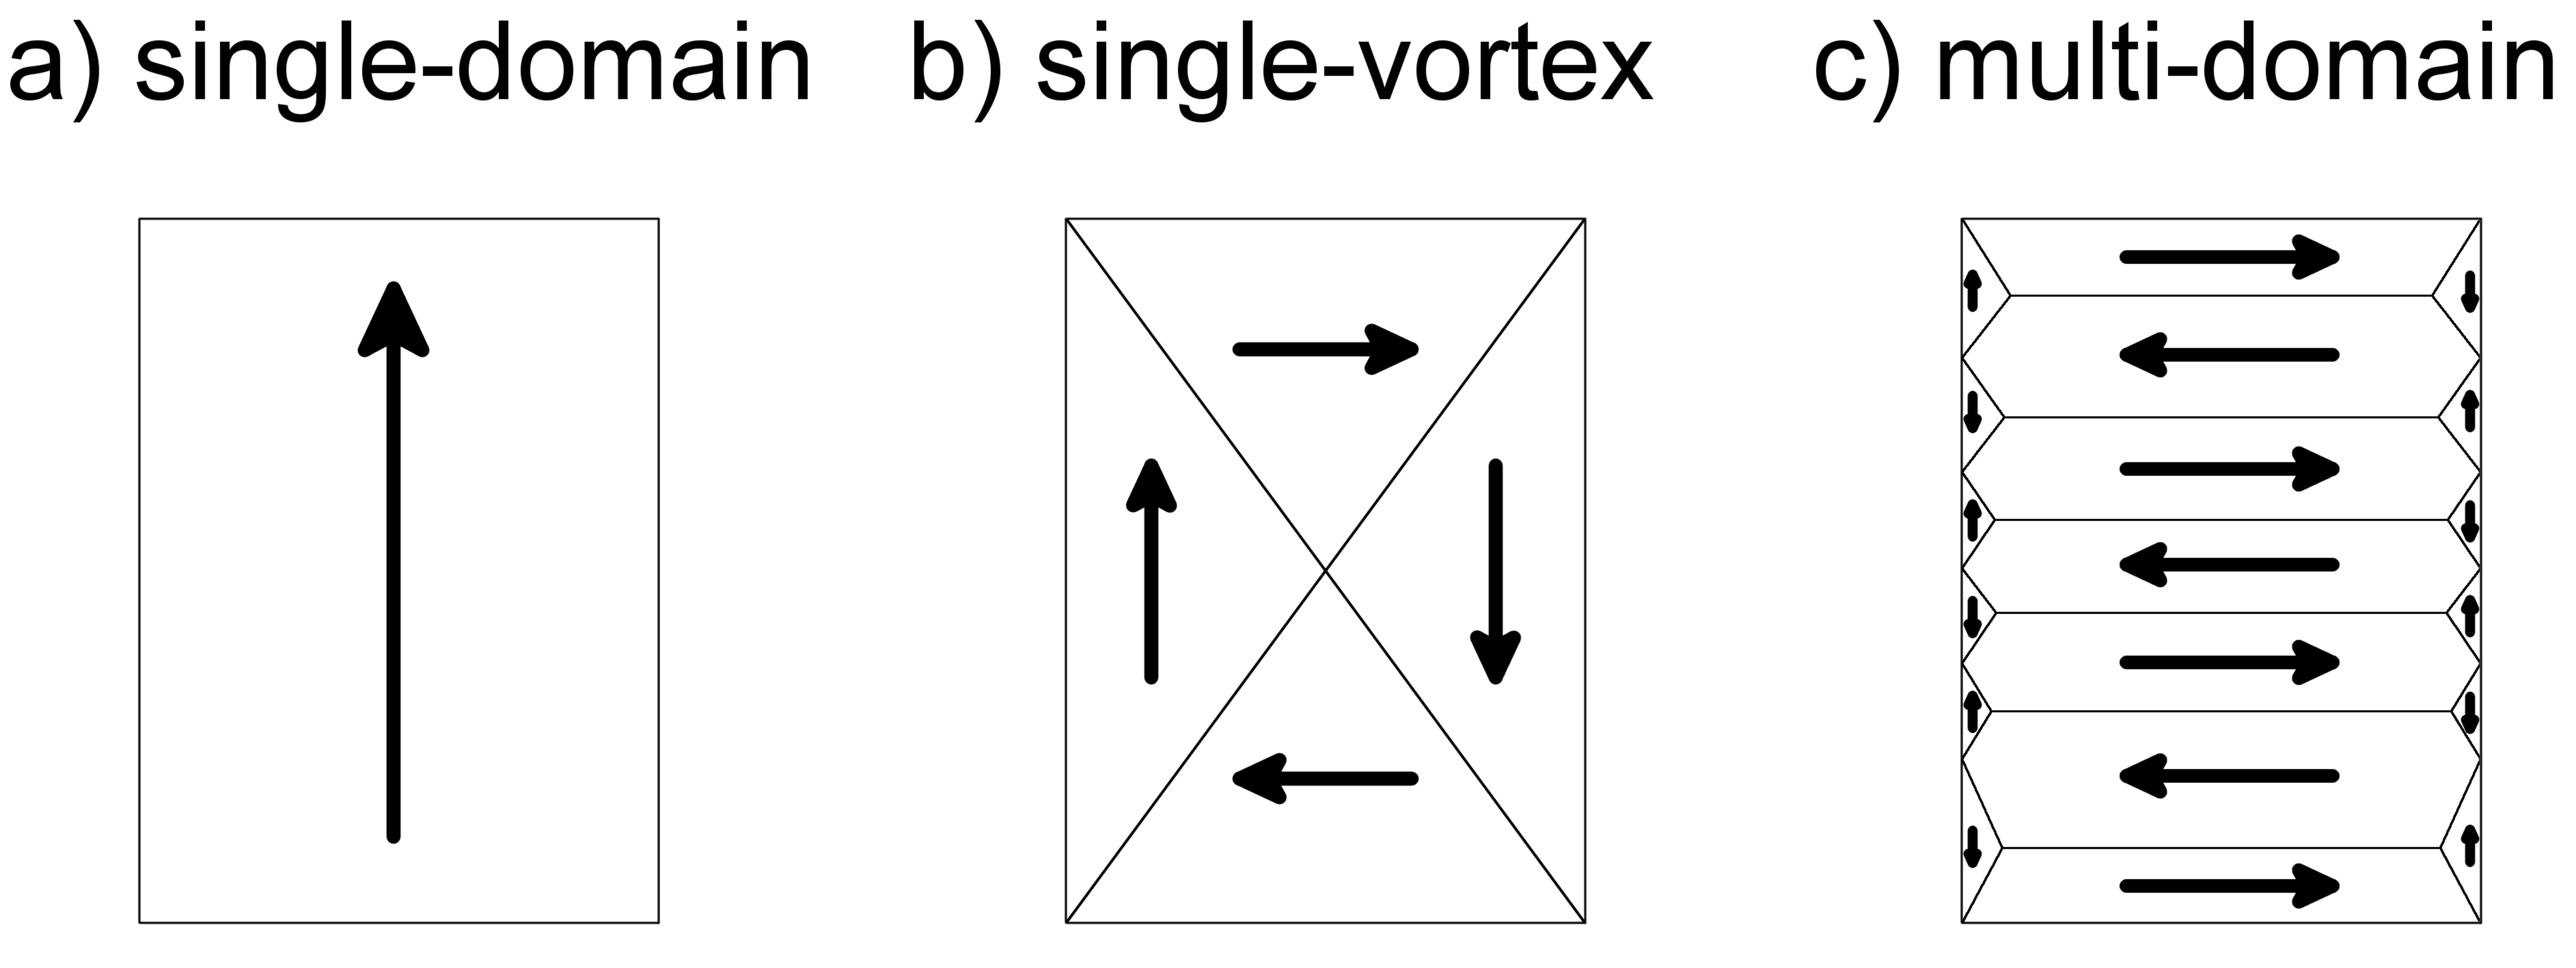
\includegraphics[width=\textwidth]{intro/figs/schematic_domains.pdf}
\caption[Domain state schematic]{Domain state schematic. Single-domain particles (a) are uniformly magnetised (highest magnetic moment). With increasing size, the magnetisation curls into a single-vortex state (b) (lower magnetic moment). In larger particles, the magnetisation is arranged in a multi-domain state (c) with regions called magnetic domains uniformly magnetised (lowest magnetic moment).}
\label{schematic_domains}
\end{figure}\par

Airborne magnetic surveys over oil fields \citep{Donovan1979} have revealed magnetic anomalies, i.e., measurable variations in the background magnetic field. \citet{Donovan1979} suggested that these anomalies are caused by the creation of authigenic near-surface magnetite in an environment of hydrocarbon seepage from the underlying reservoir. Further studies by \citet{Donovan1984}, \citet{Elmore1993} and \citet{Reynolds1993} in the U.S.A., \citet{Diaz2000}, \citet{Costanzo2006,Costanzo2012}, \citet{Gonzalez2002}, \citet{Guzman2011} in Venezuela and \citet{Liu1999}, \citet{Liu2004,Liu2006} in China have provided strong evidence for a genetic relationship between the magnetic contrasts produced by ferrimagnetic minerals near the surface and the underlying reservoir. These investigations confirm the original hypothesis \citep{Donovan1979} that the reducing environment caused by the upward seepage from the reservoirs is conducive to the formation of magnetic minerals such as magnetite and other iron oxides, greigite and other iron sulphides and depletion of minerals such as hematite \citep{Machel1991}, thus furthering the case for using a combination of aeromagnetic surveying and rock-magnetic measurements of soils and rocks for hydrocarbon prospecting.\par

Authigenic formation of magnetic minerals under hydrocarbon-producing conditions has been confirmed by \citet{Abubakar2015}; however, discussion on the exact mechanism for the formation of these minerals at different depths is ongoing. \citet{Machel1991} have identified two primary agents for the precipitation of magnetic minerals under the influence of hydrocarbon seepage. At higher temperatures and thus greater depths they propose chemical processes as the main factor while at shallower depths and lower temperatures it is argued that microbial sulphate-reducing processes are playing the larger role. \citet{Machel1991} also emphasised the difficulty in linking a magnetic anomaly to a process of hydrocarbon seepage because the precipitation of magnetic minerals can cause positive or negative anomalies---that is, peaks or dips in the geomagnetic field and the magnetic susceptibility of the soils. Nevertheless, careful analysis of the local conditions can result in the successful application of rock-magnetic measurements to hydrocarbon exploration \citep{Donovan1984,Liu2006,Emmerton2013B}. Magnetisation of oil-bearing rocks can also be used to assess the quality of oil \citep{Emmerton2013}. It was recognised by \citet{Reynolds1993} that in some cases iron sulphides are more important to the magnetic contrasts and thus to the identification of prospective oil-producing fields than iron oxides. Particularly, greigite (Fig. \ref{fram_oil}) has been identified as an authigenic mineral of the utmost importance \citep{Reynolds1993}.
\begin{figure}
\centering
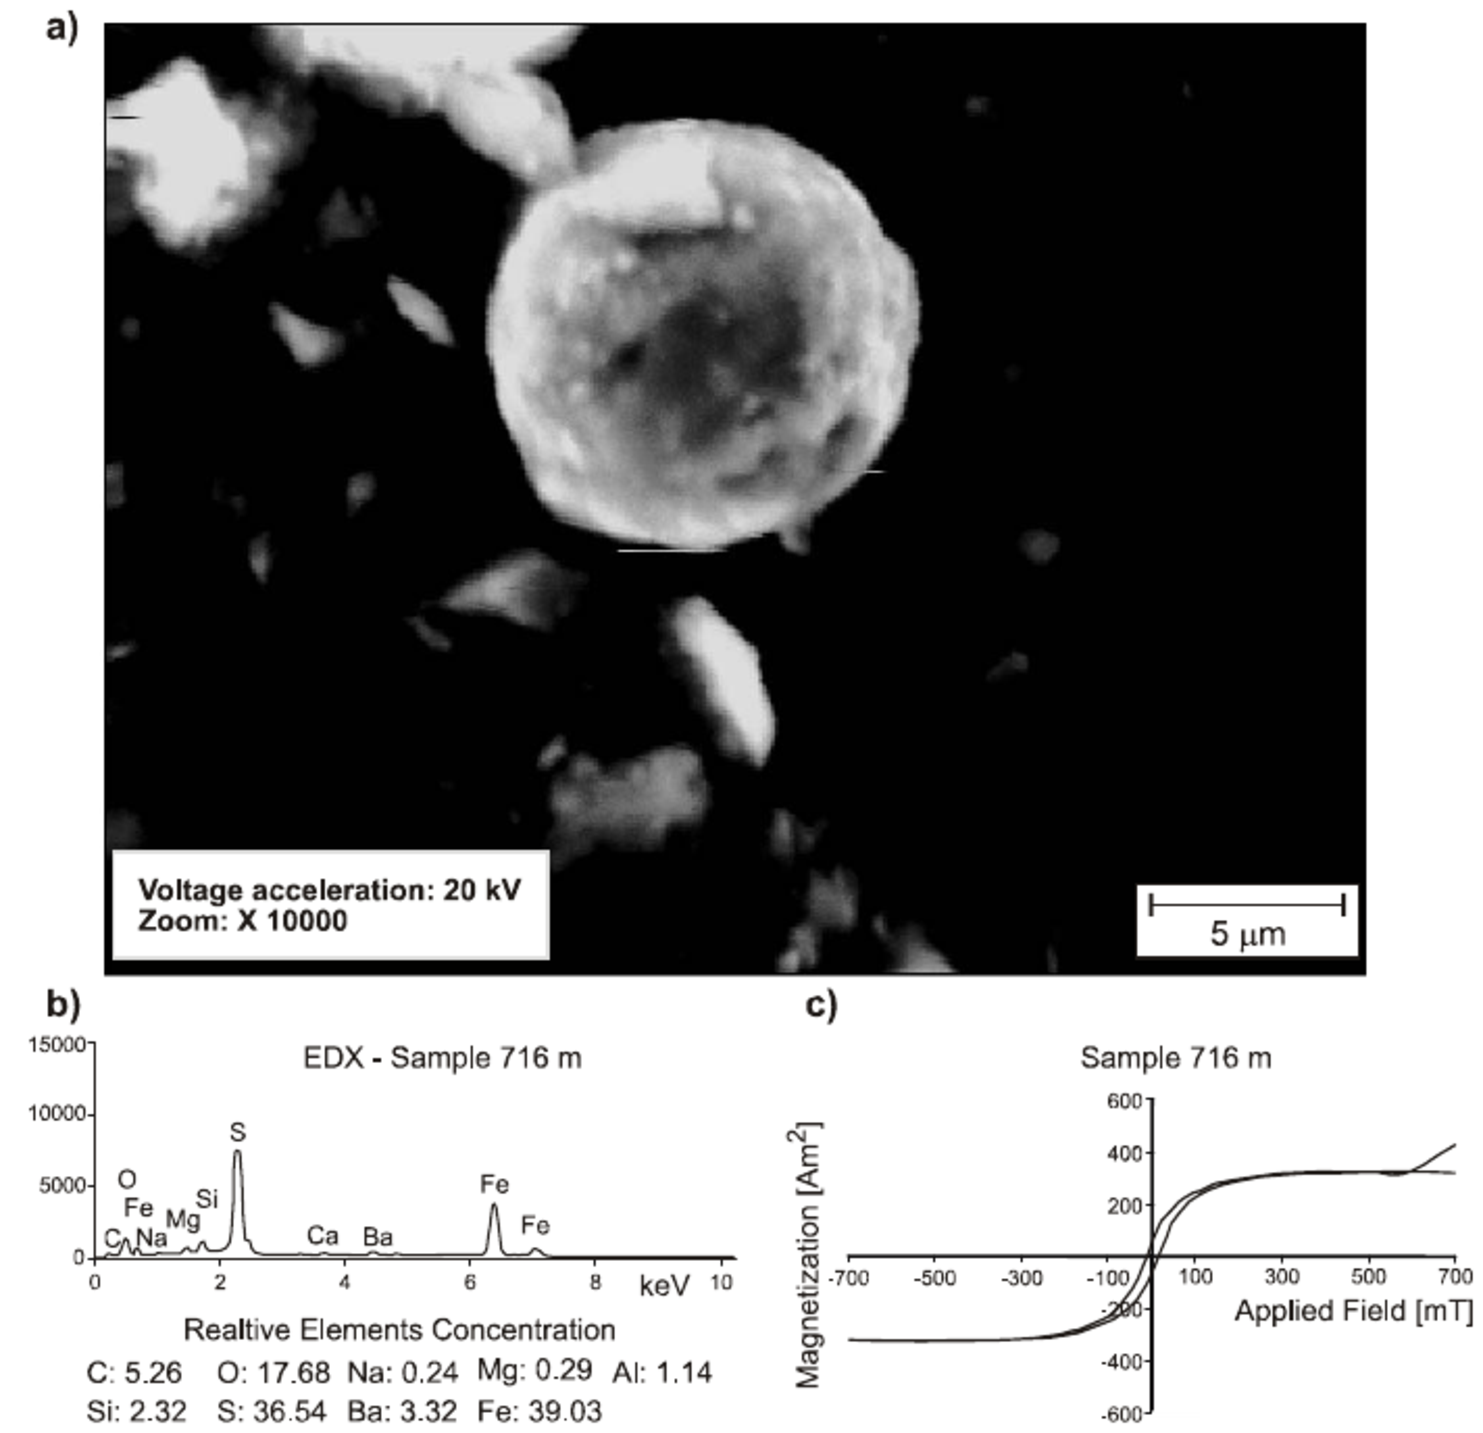
\includegraphics[width=\textwidth]{intro/figs/framboid_oil.pdf}
\caption[Greigite associated to hydrocarbon related magnetic contrasts]{Greigite associated to magnetic contrasts in hydrocarbon reservoirs. a) Scanning electron microscope micrograph and b) energy-dispersive X-ray spectroscopy analysis from the magnetic fraction of drill cuttings show spherical aggregates of minerals with high Fe and S content (likely greigite). c) Hysteresis curves for the same sample support the presence of ferrimagnetic minerals. (From \citet{Guzman2011}, reproduced with permission from the author).}
\label{fram_oil}
\end{figure}
\par

Greigite, first discovered in lacustrine sediments \citep{Skinner1964}, is an iron sulphide (Fe$_3$S$_4$) that can be thought of as the sulphide equivalent of the iron oxide magnetite (Fe$_3$O$_4$) as they have the same crystal structure only with sulphur replacing oxygen. Like magnetite, it is highly magnetic \citep{Li2014}. It is commonly formed authigenically in diagenetic anoxic sulphate-reducing sediments \citep{Roberts2011} as a precursor to pyrite \citep{Berner1984,Hunger2007}. Because of its unstable and precursory nature, its importance as a palaeomagnetic recorder has not been as readily realised as that of magnetite. However, geochemical conditions in sediments that are conducive to the long-term preservation of greigite are not uncommon \citep{Roberts2011,Roberts2015} and so, greigite is an important carrier of natural remanent magnetisation (NRM) in many systems \citep{Reynolds1994,Snowball1997,Ron2007,Roberts2010}.\par

Magnetic mineral grains that are linked to hydrocarbon seepage have sizes $\leq 30 \nm$ and thus generally in the SD range \citep{Liu2006}. In terms of morphology, it has been repeatedly found \citep{Ariztegui1996,Snowball1997,Aldana1999,Rowan2006,Roberts2010,Roberts2015} that equant grains of greigite assemble in raspberry-shaped aggregates (Fig. \ref{intro_01}) called framboids (from the French \textit{framboise} meaning raspberry). Presence of magnetic particle framboidal clusters has been linked to chemical alterations produced by hydrocarbon seepage \citep{Aldana1999} and to palaeoclimatic conditions \citep{Ariztegui1996}.\par

Given the unstable nature of greigite and the difficulties to produce synthetic samples, numerical investigations have the potential to answer important questions about greigite that can have great impact on magnetic hydrocarbon exploration and environmental magnetic studies. It is important that the fundamental magnetic parameters of greigite are precisely known to create accurate numerical models. Fabrication of higly pure synthetic greigite allowed \citet{Chang2008} to measure the saturation magnetisation $M_\text{S}$ and the exchange stiffness constant $A$; \citet{Li2014} improved the measurement of the saturation magnetisation. \citet{Winklhofer2014} measured the first estimates for the magnetocrystalline anisotropy (MCA) constants. These studies allow now for accurate models of greigite magnetisations.
\begin{figure}
\centering
\includegraphics[width=\textwidth]{intro/figs/greigite_framboids_edit.pdf}
\caption[SEM images of framboidal greigite]{Scanning electron microscopy images of iron sulphide minerals. Elongated framboids and non-framboidal pyrite aggregates that probably represent remineralisation of plant cellular matter(a, b). Images at progressively higher magnification of an iron sulphide nodule with evidence of plant matter remineralisation (c--f). The platey minerals are non-magnetic hexagonal pyrrhotite. In (e), a void within the polished surface reveals a cluster of greigite (finest-grained) and pyrite (coarser-grained) framboids that have been overgrown by pyrrhotite (platey texture). (From \citet{Roberts2015}, reproduced with permission from the author).}
\label{intro_01}
\end{figure}
\par

In this thesis, numerical methods are employed to answer some fundamental questions about the magnetic properties of greigite:
\begin{itemize}
\item How does shape and size effect the magnetic structure in sub-micronic greigite?
\item What is the critical size at which greigite can no longer be SD?
\item Can greigite carry stable magnetisations over geological scales?
\end{itemize}
Also, it is important to answer some questions on how these properties effect bulk measurements commonly used for the identification of greigite. In this thesis, the focus is on hysteresis \citep{Mayergoyz1986} and first-order reversal curve (FORC) \citep{Roberts2000} properties:
\begin{itemize}
\item What is the hysteresis and FORC signal of non-interacting SD greigite ensembles?
\item What effect does SV magnetisations have on the non-interacting FORC response?
\item What is the FORC response of framboidal aggregates of greigite?
\end{itemize}
Answers to these questions have the potential to aid identification of greigite associated with magnetic constrasts over oil reservoirs.\par

\section{The iron sulphide greigite}
\subsection{Greigite occurrence in sediments}
In sulphide-rich sediments, ubiquitous redox reactions cause magnetic iron oxide minerals like magnetite and hematite to be replaced by iron sulphides \citep{Roberts2015}, most commonly pyrite \citep{Berner1984}. Pyrite is a paramagnetic mineral, and thus does not carry a permanent magnetisation. The replacement of magnetite and hematite for pyrite has important consequences for palaeomagnetic analyses of sediments as it can cause the effective destruction of the palaeomagnetic signal \citep{Rowan2009}. This process is pervasive in continental margin marine sediments with high organic carbon contents \citep{Roberts2015}. However, if the rate of Fe$^{2{+}}$ supply exceeds H$_2$S production (e.g. by sulphate-reducing bacteria), iron sulphides that form as precursors to pyrite formation (like greigite) can be preserved \citep{Berner1984}. Greigite can form early during sediment burial \citep{Reynolds1999} or at a later stage, remagnetising the host sediment \citep{Roberts2005} depending on the chronological sequence of the availability of the reactants conducive to greigite preservation. Identification of greigite and the timing of its formation is therefore critical for the magnetic interpretation of sediments.\par

\subsection{Greigite textures: framboidal clusters}
Iron sulphide textures can provide important environmental information about the early sedimentary conditions \citep{Roberts2015}. It is, then, important to identify the texture in which greigite occurs. Among the possible greigite textures, framboidal greigite has been identified as widespread \citep{Ariztegui1996,Wilkin1997} and potentially related to hydrocarbon migration \citep{Aldana1999}.\par

Framboids are spherical aggregates of greigite nano-crystals in which all the crystallites have the same size (Fig. \ref{intro_01}). Greigite and pyrite are often found in framboidal clusters and greigite also filling the space in a less organised manner \citep{Wilkin1997,Roberts2005,Roberts2010,Rowan2006}. Framboid origin is still debated, although some conclusions have been proposed. This morphology does not require biological activity \citep{Sweeney1973,Wilkin1996} although abundance of framboidal greigite is associated with high organic content. It is argued that formation of framboidal greigite is a necessary precursor to pyrite framboids \citep{Sweeney1973,Wilkin1997}. Greigite framboids have been widely observed and the constituent nanocrystals are always finer-grained than neighbouring pyrite crystals \citep{Ariztegui1996,Roberts2005,Roberts2010,Rowan2006}. This is consistent with the pyrite framboid formation process proposed by \citet{Wilkin1997}:
\begin{enumerate}
\item nucleation of iron monosulphide (FeS, mackinawite) nanocrystals,
\item chemical alteration of these into greigite (Fe$_3$S$_4$),
\item aggregation of greigite nanocrystals with uniform sizes to form framboids,
\item replacement of greigite by pyrite (FeS$_2$).
\end{enumerate}
Alternatively, the geochemical balance between iron and sulphur can impede the replacement of greigite by pyrite, leading to greigite preservation.\par

Independently of formation mechanism, an important aspect of greigite and pyrite framboids is that the nanocrystals in all framboids have uniform particle sizes \citep{Wilkin1996}. This is a potential indication that the crystallites nucleated simultaneously, at the same growth rate and thus all under the same geochemical conditions. This is an important observation with potential applications for the timing of sulphidisation events on a geological timescale. Because of this, identification of framboidal greigite is an important problem for environmental magnetic studies. Occurences of magnetite framboids in meteoritic samples have also been observed \citep{Astafieva2004,Kimura2013}; therefore, magnetic mineral framboidal textures are widespread and identification via rock magnetic measurements is an important problem.\par

\subsection{Fundamental magnetic parameters of greigite}
The fundamental magnetic parameters of greigite used throughout this investigation are the saturation magnetisation $M_\text{S}=3.51\,\mu_\text{B}\,\text{p.c.u.}$ \citep{Li2014} or $\roughly 2.7 \times 10^5\,\text{A/m}$  which is $\roughly$11\% higher than the value previously reported by \citet{Chang2009} of $3.25\,\mu_\text{B}$ p.c.u. (and $\roughly$57\% the value of  $M_\text{S}$ for magnetite). \citet{Li2014} synthesised highly pure, high-crystallinity greigite samples on which $M(H)$ hysteresis curves were measured. The saturation magnetisation was estimated from a nonlinear fitting $M(H)=M_{\text{S}}(1-aH^{-1} + b{H^{-2}}) + cH^{1/2}$ where $a,\, b,\, c$ are constants that describe the structural inhomogeneity within the sample, the magnetic anisotropy energy, and the paramagnetic effect caused by the applied field, respectively. Microstructural inhomogeneities determine the low field response whereas the approach to saturation is determined by the anisotropy \citep{Li2014}. The obtained room-temperature value of $M_\text{S}=3.51\,\mu_\text{B}\,\text{p.c.u.}$ is lower than the value of $4\,\mu_\text{B}\,\text{p.c.u.}$ predicted from a purely ionic model \citep{Coey1970}, this is due to the degree of covalency of the Fe--S bond as well as the possible canting of surface spins induced by surfactant molecules bonded to the surface \citep{Li2014}. Of the magnetic parameters used for the purposes of this work, the value of the saturation magnetisation is the most accurate.\par

\citet{Winklhofer2014} used ferromagnetic resonance spectroscopy to estimate the anisotropy constants. They obtained a (first) cubic MCA constant $K_1=-1.7\times10^4\,\text{J}/\text{m}^3$ and negligible second MCA constant $K_2$ to $K_1$ ratio, i.e., the easy axes are the $<$111$>$. The data was consistent, as well, with a positive value for $K_1$ and large $K_2\approx 3K_1$ and thus $<$100$>$ easy axes; however, there is indirect \citep{Winklhofer2014} and direct \citep{Li2014} evidence favouring the anisotropy model with negative $K_1$ which we use throughout this work.\par

The exchange stiffness constant was estimated by \citet{Chang2008} to be $A=2\times10^{-12}\,\text{J}/\text{m}$. The exchange energy in a ferrimagnet is related to the spin wave stiffness. Experimental observation of spin waves can be achieved by several methods, e.g., inelastic neutron scattering and spin wave resonance. These experimental techniques require, however, relatively large, uniform crystals on which to observe spin wave propagation. Since fabrication of such samples is as yet impossible for greigite, \citet{Chang2008} measured the saturation magnetisation (in a field of $5\,\text{T}$) of powdered greigite samples at low temperatures. Using the spin wave expansion of the spontaneous magnetisation for low temperatures $M(T)=M_{\text{S}}(1-CT^{3/2})$ \citep{Bloch1932}, where $C$ is a function of the spin wave stiffness, they were able to fit the data and obtain an estimate of the spin wave stiffness and therefore the exchange stiffness constant. Determination of the spin wave stiffness through different approaches like inelastic neutron scattering \citep{Torrie1967}, low-temperature heat capacity \citep{Kenan1963} and low-temperature $M_{\text{S}}$ measurements \citep{Aragon1992}, however, has been known to produce variable results for magnetite \citep{Chang2008}. This places a degree of uncertainty on this measurement for greigite that is hard to quantify in the absence of measurements acquired through means other than low-temperature saturation magnetisation.\par

Chemical alteration of greigite at high temperatures has made difficult to measure accurately the Curie temperature; however, there is strong evidence for a Curie temperature $T_\text{C}>620\,\text{K}$ \citep{Roberts2010}. The exchange energy is directly related to $T_\text{C}$; within a mean field approximation \citep{Kouvel1956}:
\begin{equation}
T_\text{C} = \frac{4\sqrt{2} J_\text{AB}}{K_\text{B}}\sqrt{S_\text{A}S_\text{B}(S_\text{A}+1)(S_\text{B}+1)},
\end{equation}
where $K_\text{B}$ is Boltzmann's constant, $J_\text{AB}$ is the exchange integral between A- and B-sites and $S_\text{A},\, S_\text{B}$ the spin magnetic moments of sites A and B, respectively. Plugging in the relatively low value of $J_\text{AB}\approx 1\,\text{meV}$ measured by \citet{Chang2008} and $S_\text{A}=1.54$, $S_\text{A}=1.63$ \citep{Chang2009} predicts a low $T_\text{C} \approx 260-287 \, \text{K}$. This suggests the uncertainty in the measurement of $A$ by \citet{Chang2008} is significant. A value of $J_\text{AB}=2.31\,\text{meV}$ results in a $T_\text{C}\approx 620\,\text{K}$. However, mean field approximations tend to overestimate the Curie temperature, so the value of the exchange integral $J_\text{AB}$ could be up to 4 times the value reported by \citet{Chang2008}. Throughout this work the value of \citet{Chang2008} is used. Increased values of $A$ have the effect of increasing the domain wall width and thus the critical size $d_0$; a calculation of the SD to SV critical size $d_0$ was done for values $A=4\times10^{-12}\,\text{J}/\text{m}$ and $A=8\times10^{-12}\,\text{J}/\text{m}$ (Chapter \ref{ch:res-1}) to quantify this effect. Changes in the exchange stiffness constant have little effects on the coercivities of SD and possibly SV grains. Uncertainty in this parameter can modify the absolute values of some of the magnetic properties simulated in this work, however, the physics should remain mostly unaffected.\par

\section{Magnetism and matter}
For the purposes of the thesis, a brief review of fundamental concepts of magnetism follows.\par
 
\subsection{Fundamentals of magnetism}
The magnetic induction field $\boldsymbol{B}$, like the electric field $\boldsymbol{E}$, is defined by its effect on a \textit{test particle}, namely, the Lorentz force \citep{Feynman}:
\begin{equation}\label{lorentz}
\boldsymbol{F}_\text{Lorentz} = q(\boldsymbol{E} + \boldsymbol{v}\times\boldsymbol{B}),
\end{equation}
where $q$ is the electrical charge of the test particle and $\boldsymbol{v}$ its velocity. The force a magnetic $\boldsymbol{B}$ field exerts on a moving electrical charge is perpendicular to both its velocity and to the field itself. From Eq. \ref{lorentz}, the units of $\boldsymbol{B}$ are $\text{N}/(\text{C}\cdot\frac{\text{m}}{\text{s}})$, this physically meaningful unit (one Newton of force per charge of one Coulomb moving at one meter per second) is called Tesla, with symbol $\text{T}$.\par

When describing magnetic fields, a distinction between the magnetic induction $\boldsymbol{B}$ and the magnetic field $\boldsymbol{H}$ is made. These denominations, however, are of historical character; it can be proved that the fundamental field is the induction field $\boldsymbol{B}$ \citep{Feynman}. In a vacuum, $\boldsymbol{B}$ and $\boldsymbol{H}$ coincide in direction. In the SI the magnetic and induction fields differ by a scalar factor $\mu_0$, the \textit{magnetic constant}, also known as the vacuum permeability or permeability of free space:
\begin{equation}
\mu_0 = \frac{B_{\text{vacuum}}}{H_{\text{vacuum}}} = 4 \pi \times 10^{-7} \, \text{T}\cdot\frac{\text{m}}{\text{A}}.
\end{equation}
Although the names vacuum permeability and permeability of free space are still widespread it is preferable to use the name magnetic constant since it reflects the fact that it is a defined value and not a measurement.\par

The description of magnetic fields is analogue to that of electrical fields. Although, unlike the situation in electricity, there are no magnetic charges, only magnetic dipoles \citep{Feynman}. The induction due to a wire carrying a current $I$ (generally varying along the path) at a point $\boldsymbol{r}$ can be calculated from the Biot-Savart law:
\begin{equation}
\boldsymbol{B}(\boldsymbol{r}) = \frac{\mu_0}{4\pi} \int_C \frac{I\, \text{d}\boldsymbol{l}\, \times \, \boldsymbol{r}}{r^3},
\end{equation}
where $\text{d}\boldsymbol{l}$ is a differential element of length along the wire in the direction of the current. The integral is carried out along a line, usually but not necessarily a closed curve.\par

In general, it is more interesting and important to consider magnetism in the presence of matter. A material is composed of atoms, which individually may hold a permanent magnetic dipole moment $\boldsymbol{\mu}$ (with units $\text{A}\cdot \text{m}^2$). The \textit{magnetisation} vector field $\boldsymbol{M}$ (with constant norm $|\boldsymbol{M}|=M_\text{S}$) is the spatial average of a myriad of these individual atomic dipole moments over a suitable volume. Therefore, $\boldsymbol{M}$ accounts for the contribution of atomic magnetic moments to the total field. In the SI units we have
\begin{equation}
\boldsymbol{B} = \mu_0 (\boldsymbol{H}+\boldsymbol{M});
\end{equation}
$\boldsymbol{H}$ and $\boldsymbol{M}$ have the same units, the Ampere per meter $\text{A}/\text{m}$. The meaning of this unit is somewhat obscured, but made evident if written in the form $\text{A}/\text{m} = \text{A}\cdot\text{m}^2/\text{m}^3$, i.e., this unit can be thought of as a density of magnetic moments.\par

\subsection{Diamagnetism and paramagnetism}
Magnetism in matter can be broadly categorised into three phenomena: diamagnetism, paramagnetism and ferromagnetism. Diamagnetism and paramagnetism are of little importance to this work so will be only briefly described.\par

Diamagnetism is a property of all matter. It is the smallest effect and is a tendency of a material to oppose an external magnetic field. An external magnetic field exerts a Lorentz force on the bound electrons that causes them to precess like a gyroscope. This is called Larmor precession and is equivalent to an electric current producing a magnetic moment in the direction opposed to the external $\boldsymbol{B}$ field. Water is a common example of a highly diamagnetic material.\par

Paramagnetism is a partial alignment of the atomic magnetic moments of the atoms in a material with an external $\boldsymbol{B}$ field. It is only thermal noise that prevents a perfect alignment of the atomic magnetic moments with the external field, therefore this is a highly temperature dependent phenomenon. Nevertheless, at ordinary temperatures, paramagnetism outweighs diamagnetism by a factor greater than 10.\par

In both diamagnetism and paramagnetism a magnetisation is induced by an external field. The rate at which the magnetisation is acquired with respect to the applied field is called the \textit{magnetic susceptibility} $\chi = \frac{\text{d}\boldsymbol{M}}{\text{d}\boldsymbol{H}}$, in general a tensor.\par

\subsection{Ferromagnetism}
A ferromagnetic material, in contrast with diamagnetic and paramagnetic materials, can retain a (non-saturated) remanent magnetisation in the absence of an external field. In the presence of a relatively weak external field, ferromagnetic materials acquire magnetisations thousands of times stronger than paramagnetic materials. To reconcile these two observations, \cite{Weiss1906} proposed that in ferromagnetic materials there exist magnetic domains, regions which are locally magnetised to saturation, brought about by an \emph{ad-hoc} molecular field; when there is an external field, domains aligned with the field would grow and/or the domains would rotate with the field and when the field is removed the domains would return to random alignments thereby reducing the net magnetisation of the body. Although domain theory was succesful in explaining important aspects of ferromagnetic behaviour, the theory was unsatisfying as it did not explain the origin of the molecular field \citep{Kittel1949}.

Ultimately, ferromagnetism is a phenomenon that cannot be explained solely by classical physics. At the core is the quantum-mechanical concept of exchange coupling, a phenomenon with no classical counterpart \citep{Heisenberg1926}. The origin of ferromagnetism is the alignment of atomic moments (electron spins) by quantum exchange forces. However, in a narrower sense, ferromagnetic materials are those in which \emph{all} the atomic moments share the same alignment. There is a class of materials in which the quantum exchange forces create anti-parallel alignments between atomic moments in different sublattices. When the net magnetic moment of one sublattice is smaller than that of the other, there remains a net moment: these are the ferrimagnetic materials. When the magnetic moments of the different sublattices cancel there is no net magnetic moment: these are the antiferromagnetic materials. Throughout the thesis, the term ferromagnetism is used in a broad sense to include ferrimagnetic behaviour.\par

Exchange coupling is hindered by thermal noise, i.e., ferromagnetic behaviour weakens with increasing temperature. There is a threshold temperature beyond which thermal fluctuations destroy all magnetic ordering and the material becomes paramagnetic; this is the Curie temperature $T_\text{C}$, characteristic of a ferromagnetic material.\par

\citet{Landau1935} obtained a continuum expression for the exchange energy. The main result in \citet{Landau1935} was the theoretical proof that inside a ferromagnetic material there are regions that are magnetised to saturation: the magnetic domains, and that between these domains exist regions where the magnetisation continuously rotates from the direction of one domain to that of the other; these are called \textit{domain walls}. The calculation of \citet{Landau1935} of magnetic domain size and domain wall width and speed of propagation was the first micromagnetic calculation \citep{Brown}.

\section{Micromagnetics}\label{mmsection}
\citet{Brown} recognised that there was a need for a robust theory on a scale large enough to treat ferromagnetic bodies as a a continuum and small enough to capture the magnetic structure at sub-micron lengths. He called such a theory micromagnetics. The seminal work of \citet{Landau1935} and that of \citet{Brown} are the theoretical basis from which micromagnetics emerged. Micromagnetics is the theory that bridges the fundamental quantum-mechanical picture and the effective macroscopic theory of Maxwell equations. The main goal of micromagnetics is to obtain a configuration of the magnetisation vector $\boldsymbol{M}$ in a ferromagnetic material.\par

\subsection{Magnetic Gibbs free energy}
There are two main approaches to micromagnetism. One is to obtain a configuration of the magnetisation in a ferromagnetic material by minimising the magnetic Gibbs free energy. The other is to solve a partial differential equation (PDE) that describes the dynamics of the magnetic moments; this equation was derived by \citet{Landau1935} and improved by \citet{Gilbert2004} to include damping effects, the Landau-Lifshitz-Gilbert (LLG) equation.\par

It is known from thermodynamics that starting from a nonequilibrium state the evolution of a system can only be such that its Gibbs free energy diminishes. So, by an explicit formulation of the different energies contributing to the total magnetic Gibbs free energy it is possible to find a configuration that is either a local energy minimum (LEM) or global energy minimum (GEM). One of the biggest contributions of micromagnetics to our understanding of magnetic phenomena in matter is that it is quite common for a material to be in a LEM configuration rather than GEM. This is the cause of magnetic hysteresis and magnetic remanence. Disregarding thermal effects and magnetostrictive forces, four magnetic energies contribute to the total. There are microscopic contributions like the exchange energy and the MCA energy. Also macroscopic contributions like the magnetostatic self-energy and the external field energy. The external field is independent of the magnetisation and the exchange and anisotropy energies are short range so these are very easy to calculate. The magnetostatic self-energy, i.e., the interaction between the magnetic moments in the material and the stray field the magnetic body produces is a long range, non-local interaction. This energy creates a demagnetising effect.\par

We can write the total magnetic Gibbs free energy $E_\text{G}$ as the integral of the sum of energy densities $\phi$ associated with these effects \citep{Brown}:
\begin{equation}\label{gibbs0}
E_{\text{G}} = \int_{\Omega} (\phi_{\text{exchange}} + \phi_{\text{anisotropy}} + \phi_{\text{stray}} + \phi_{\text{external}})\, \text{d}^3\boldsymbol{r},
\end{equation}
where $\Omega$ is the ferromagnetic volume and $\text{d}^3\boldsymbol{r}$ the volume differential.\par

The exchange energy is a quantum-mechanical phenomenon wherein the exchange of inner shell electrons between neighbouring atoms results in spin-exchange coupling. The continuum expression was obtained by \citet{Landau1935} and found to be proportional, up to a constant, to the square of the gradient of the magnetisation distribution:
\begin{equation}
\phi_{\text{exchange}} = A | \nabla \boldsymbol{m} |^2,
\end{equation}
where $A$ is the exchange stiffness constant and $\boldsymbol{m}$ is the reduced magnetisation vector, i.e., $\boldsymbol{m}$ is a unit vector in the direction of the magnetisation. This energy density is minimised for uniform magnetisations, therefore, the effect of the exchange energy is to homogenise the distribution of moments.\par

MCA energy is due to the atomic configuration of a crystalline material. The specific arrangement of atoms in the crystal can cause some directions to be easier for the moments to align with \citep{Kittel1949}. These directions are called easy axes. The anisotropy energy of a cubic crystal is given by:
\begin{equation}
\phi_{\text{anisotropy}}=\frac{K_1}{2}\sum_{i\neq j}\gamma_i^2\gamma_j^2 + K_2\prod_i\gamma_i^2,
\end{equation}
where $\gamma_i$ are the magnetisation direction cosines and $K_1$, $K_2$ the first and second anisotropy constants. In terms of the reduced magnetisation vector components, this can be written as:
\begin{equation}
\phi_{\text{anisotropy}}=K_1(m_x^2m_y^2+m_y^2m_z^2+m_z^2m_x^2) + K_2m_x^2m_y^2m_z^2.
\end{equation}
The effect of the MCA energy is a tendency for the magnetic moments to align with the easy axes of magnetisation.\par

The external field energy is the potential energy associated with the interaction of the magnetic moments with an external field:
\begin{equation}
\phi_{\text{external}} = -\boldsymbol{M} \cdot \boldsymbol{B}_{\text{external}},
\end{equation}
where $\boldsymbol{B}_{\text{external}}$ is an external magnetic induction field. This energy tends to align the magnetic moments with the external field.\par

The magnetostatic self-energy is due to the magnetostatic interaction each magnetic moment has with each other. Because in a numerical micromagnetic model there can be hundreds of thousands of individual magnetic moments (mesh/grid points), this is energy is the most numerically expensive to calculate; many methods have been devised to avoid calculating this interaction for each moment, most of these based on the magnetic scalar potential.\par

A partial differential equation for the magnetic potential $\varphi$ is formulated of the form:
\begin{equation}\label{potential}
\nabla^2 \varphi(\boldsymbol{r}) =
\begin{cases}
4\pi\nabla \cdot \boldsymbol{M}, & \text{for }\boldsymbol{r} \in \Omega \\
0,                           & \text{for }\boldsymbol{r} \in \mathbb{R}^3 / \boldsymbol{\Omega};
\end{cases}
\end{equation}
with boundary conditions on the surface $\partial \Omega$:
\begin{align}\label{boundaries1}
\left. \left[ \varphi \right]\right|_{\partial \Omega} &= 0, \\
\left. \left[ \frac{\partial \varphi}{\partial \boldsymbol{\hat{n}}} \right]\right|_{\partial \Omega} &= -4\pi \boldsymbol{M} \cdot \boldsymbol{\hat{n}}, \label{boundaries2}
\end{align}
where $\left. \left[\cdots \right]\right|_{\partial \Omega}$ denotes a discontinuity across the boundary (surface) and $\boldsymbol{\hat{n}}$ an outward-pointing surface-normal unit vector. Also, a condition:
\begin{equation}\label{boundary}
\lim_{|\boldsymbol{r}| \to \infty} \varphi(\boldsymbol{r}) = 0
\end{equation}
must be met. Solving this sytem for $\varphi$ is sufficient to calculate the stray field from:
\begin{equation}
\boldsymbol{B}_\text{stray} = -\mu_0 \nabla \varphi.
\end{equation}\par

One of the principal difficulties in solving Eq. \ref{potential} is the limit condition (Eq. \ref{boundary}) because in numerical calculations it is impossible to formally evaluate the potential at infinity. \citet{Imhoff1990} proposed a transformation method that requires space surrounding the ferromagnetic body to be meshed into two concentric shells. The potential is mapped on the outer shell to infinity to satisfy the boundary conditions. A hybrid finite-element method (FEM) and boundary-element method (BEM) formulation \citep{Fredkin1990} does not require free space to be meshed, at the cost of the mathematical complexity involved in the hybrid scheme. In this scheme, the scalar magnetic potential is split $\varphi = \varphi_1 + \varphi_2$, where for $\boldsymbol{r} \in \Omega$, $\varphi_1$ is the solution to the inhomogenous Neumann problem:
\begin{equation}
\nabla^2 \varphi_1 = 4 \pi \nabla \cdot \boldsymbol{M}
\end{equation}
with the boundary condition
\begin{equation}
\left. \frac{\partial \varphi_1}{\partial \boldsymbol{\hat{n}}} \right|_{\partial \Omega} = 4 \pi \boldsymbol{M} \cdot \boldsymbol{\hat{n}},
\end{equation}
and $\varphi_1$ is defined $\varphi_1 = 0$ for $\boldsymbol{r} \in \mathbb{R}^3 / \Omega$. With this, $\varphi_2$ satisfies:
\begin{equation}
\nabla^2 \varphi_2 = 0,
\end{equation}
and from the boundary conditions (Eqs. \ref{boundaries1}, \ref{boundaries2}), there are conditions at the boundary:
\begin{align}
\left. \left[  \varphi_2 \right] \right|_{\partial\Omega} &= \varphi_1, \\
\left. \left[  \frac{\partial\varphi_2}{\partial\boldsymbol{\hat{n}}} \right] \right|_{\partial\Omega} &= 0;
\end{align}
a condition $\lim_{|\boldsymbol{r}| \to \infty} \varphi_2 = 0$ is also required. In practice, $\varphi_1$ is determined with a FEM which gives the boundary conditions to determine $\varphi_2$ via BEM.\par

The magnetostatic self-energy creates a demagnetising effect, that is, the field $\boldsymbol{B}_{\text{stray}}$ produced by the magnetisation distribution opposes the magnetisation. It is also the phenomenon that has the principal role in the domain structure of large particles. When this demagnetising field is calculated, the magnetostatic self-energy can be expressed as \citep{Brown}:
\begin{equation}
\phi_{\text{stray}} = -\frac{1}{2}\boldsymbol{M}\cdot\boldsymbol{B}_{\text{stray}},
\end{equation}\par
where the factor $1/2$ accounts for the interaction between all magnetic dipoles being counted twice when calculating $\boldsymbol{B}_\text{stray}$.\par

With these expressions for the energy densities, Eq. \ref{gibbs0} can now be rewritten as:
\begin{multline}
E_{\text{G}} = \int_{\Omega} \left( A| \nabla \boldsymbol{m} |^2  + K_1(m_x^2m_y^2+m_y^2m_z^2+m_z^2m_x^2) + K_2m_x^2m_y^2m_z^2 \right. \\
\left. - \boldsymbol{M} \cdot \boldsymbol{B}_{\text{external}} - -\frac{1}{2}\boldsymbol{M}\cdot\boldsymbol{B}_{\text{stray}} \right) \, \text{d}^3\boldsymbol{r}.
\end{multline}
A system out of equilibrium is spontaneously driven to diminish its free energy. The aim of a micromagnetic algorithm is to obtain a distribution of the magnetisation in equilibrum. \citet{Fischbacher2017} describes energy minimisation algorithms for the micromagnetic energy functional. \citet{Brown} proposed a variational method based on the variational derivative of the total energy with respect to the magnetisation. In equilibrium, the variation of the free energy vanishes
\begin{equation}
\frac{\delta E_{\text{G}}}{\delta\boldsymbol{m}} = 0.
\end{equation}
This leads to Brown's equation:
\begin{equation}
\boldsymbol{m} \times \left( \frac{2A}{M_\text{S}}\nabla^2\boldsymbol{m} + \boldsymbol{B}_\text{anisotropy} + \boldsymbol{B}_{\text{external}} + \boldsymbol{B}_{\text{stray}} \right) = 0,
\end{equation}
with $\boldsymbol{B}_\text{anisotropy} = \frac{1}{M_\text{S}}(2K_1m_x(1-m_x^2)+2K_2m_y^2m_z^2m_x)\ihat+(2K_1m_y(1-m_y^2)+2K_2m_z^2m_x^2m_y)\jhat+(2K_1m_z(1-m_z^2)+2K_2m_x^2m_y^2m_z)\boldsymbol{\hat{k}}$. This means that in equilibrium the magnetisation is parallel to an effective field:
\begin{equation}
\boldsymbol{B}_{\text{eff}} = \frac{2A}{M_s}\nabla^2\boldsymbol{m} + \boldsymbol{B}_\text{anisotropy} + \boldsymbol{B}_{\text{external}} + \boldsymbol{B}_{\text{stray}}=\mu_0 \boldsymbol{H}_\text{eff},
\end{equation}
and so, the torque (analogue) acting on the magnetic moments vanishes $\boldsymbol{m} \times \boldsymbol{B}_{\text{eff}} = 0$. This is the motivation to use a dynamical equation involving the torques produced by the effective field as an alternative to energy minimisation.\par

\subsection{The Landau-Lifshitz-Gilbert equation}
Finding an equilibrium magnetisation via energy minimisation (Eq. \ref{gibbs0}) may not always result in physically meaningful distributions. This is because in micromagnetic systems, the energy landscape is usually very complicated and contains many local maxima, minima and saddle points. A more physical approach is finding a solution to the dynamical problem. However, this is numerically more expensive than energy minimisation. The motion of a magnetic moment is mainly due to the Larmor precession around its local field. The Gilbert equation \citep{Gilbert2004} describes this precession and considers damping effects with a single damping constant:
\begin{equation}
\frac{\partial \boldsymbol{M}}{\partial t} = -\gamma\boldsymbol{M}\times\boldsymbol{H}_\text{eff} + \alpha\boldsymbol{M}\times\frac{\partial\boldsymbol{M}}{\partial t},
\end{equation}
where $\gamma = 2.210173 \times 10^5 \frac{\text{m}}{\text{A}\cdot\text{s}}$ is the gyromagnetic ratio and $\alpha$ a phenomenological damping parameter, characteristic of the material \citep{Gilbert2004}. An equivalent formulation is the LLG equation:
\begin{equation}
\frac{\partial\boldsymbol{M}}{\partial t} = -\gamma^{'} \boldsymbol{M}\times\boldsymbol{H}_\text{eff} - \frac{\alpha\gamma^{'}}{M_\text{S}} \boldsymbol{M}\times(\boldsymbol{M}\times\boldsymbol{H}_\text{eff}) \, ,
\end{equation}
with $\gamma^{'} = \gamma / (1+\alpha^2)$.

\subsection{Micromagnetic modelling}
Although the fundamentals of micromagnetic theory were laid out, analytical treatment of the micromagnetic equations was limited to simple cases \citep{Landau1935,Brown1940,Kittel1949}. In order to investigate more complex situations it is necessary to turn to approximate methods. Numerical simulations of the micromagnetic equations are, in the most general case, numerically very expensive, specially the calculation of the long-range nonlinear demagnetising energy due to magnetostatic dipolar interactions. This constrained the early numerical investigations to one- or two-dimensional rotations of the dipoles as well as geometries \citep{Brown1965,Labonte1969,Stapper1969,Aharoni1986,Fredkin1987,Zhu1988}. Although useful to probe the stability of ferromagnetic crystals with palaeomagnetic implications \citep{Moskowitz1979,Moon1984,Enkin1987}, these constrained simulations are very limited as there is no doubt that the true nature of spin structures in ferromagnetic crystals is three-dimensional.\par

\citet{Williams1989} conducted the first unconstrained three-dimensional simulations of single magnetite cubic grains, confirming the critical size of single domain magnetite grains using a conjugate gradient method for minimising the energy. Their method consisted in subdividing a cubic ``sample'' of magnetite into further cubes within the exchange length of the material. Inside each of the cubic cells the magnetisation is the average over a very large number of atomic spins and is represented by a magnetic dipole $\boldsymbol{\mu}$ at the center of the cube. The magnitude of all the dipoles is constant but their directions are allowed to vary. Already in a sample divided into $12\times 12\times 12$ cells, a direct calculation of the demagnetising energy needs around 1.5 million interaction calculations per iteration. Rewriting the demagnetising energy in the manner of \citet{Rhodes1954} they were able to reduce the computation significantly and solve for up to $22\times 22\times 22$ subcubes.\par

While the exchange, anisotropy and external field energy are local and easily calculated, it is the nonlocal dipolar magnetostatic interactions that are the principal obstacle in scaling up simulations. Much of the effort in micromagnetic research has been directed towards creating ever more efficient ways to calculate the demagnetising energy. \citet{Fabian1996} and \citet{Wright1997} developed and applied finite difference (FD) methods based on a fast Fourier transform to calculate the demagnetising energy. This, along growing computing capabilities, has allowed micromagnetics to tackle larger, more complex models \citep{Williams1998}. Nevertheless, FD methods restrict the model geometries to cuboid (rectangular prisms more generally) shapes that, while useful, are somewhat unrealistic shapes for most magnetic minerals.\par

FEMs have the advantage of being more flexible in the geometries that can be modelled; in fact, they allow for arbitrary shapes. This is because the spatial domain is discretised into tetrahedral so-called elements to create an unstructured mesh. This advantage comes at the cost of higher mathematical complexity. In FEMs, to solve a PDE, it is transformed to its \emph{weak form}; the weak form is obtained by multiplying the equation by a so-called test function from a suitable function space and integrating the equation via integration by parts. The solution is found in terms of so-called trial functions; in each node $i$ of the mesh the solution $u_i$ is postulated as a linear combination of the trial functions, e.g., $u_i=a_i\psi_1 + b_i\psi_2$, usually $\psi_j$ are linear `hat' functions. Then, an algebraic equation is formed for each node in the mesh to produce a large system of linear equations for the coefficients $a_i,\,b_i$ which is solved by an appropriate algebraic numerical method. The geometric flexibility of FEMs allows the modelling of mineral grains with complex morphologies (e.g. \citet{Williams2010}). For producing the FEM tetrahedral meshes, the proprietary software \emph{Trelis} has been used.\par

The capabilities of today's computers allows to simulate not only single grains but clusters of them that interact magnetostatically with each other. This once untractable problem has been proved to be crucial and influence the critical sizes of single domain grains. \citet{Muxworthy2003}, \citet{Muxworthy2004} and \citet{Muxworthy2006} used a FD method and investigated the effect of magnetostatic interactions between magnetite grains. \citet{Muxworthy2013} used the more recently measured \citep{Chang2008} magnetic parameters of highly pure greigite to investigate the intergrain influence in chains of greigite and its implications for magnetosome crystals, i.e., chains biomineralised by magnetotactic bacteria \citep{Lefevre2011}. However, newer, more accurate values of the magnetic parameters of greigite \citep{Li2014} have since become available. These investigations can be furthered by FEM models of more realistic geometries. In this work, the bulk of micromagnetic simulations have been carried out using the open-source program \emph{MERRILL} \citep{OConbhui2017}. This package, written in FORTRAN, uses a hybrid FEM/BEM formulation for calculation of the stray field \citep{Fredkin1990}, which makes it particularly useful for problems consisting of several non-joined ferromagnetic bodies. A number of simulations (Chapter \ref{ch:res-1}) were performed using the parallelised FEM package \emph{DUNLOP} \citep{Nagy2016}. This package, written in C++ and Python, uses a transformation method to calculate the stray field \citep{Imhoff1990}. Because of this, this package can tackle large single-body problems.\par

\section{Brief introduction to the thesis}
In Chapter \ref{ch:res-1}, the zero-field size dependence of the magnetic structure of greigite is investigated for a variety of naturally occurring shapes via a micromagnetic FEM. A nudged elastic-band (NEB) method \citep{Fabian2017} is used to calculate minimal action paths between minimal energy states for a variety of shapes and sizes. This allows calculation of the stability of a magnetisation, with implications for palaeomagnetic studies.\par

A simplified numerical model is developed in Chapter \ref{ch:res-2} to study the hysteresis of small greigite grains in a SD state. A spherical magnetic particle is essentially treated as a magnetic dipole; a gradient method is used to find the energy minimum in an applied field. This model is used to study the FORC diagrams produced by randomly oriented dispersions of non-interacting ideal SD greigite (and iron as another relevant application).\par

A micromagnetic model is used to study the FORC response of randomly oriented non-interacting particle dispersions of greigite with a variety of sizes in Chapter \ref{ch:res-3}. The FORC signal of dispersions of particles with non-uniform, vortex magnetisations is investigated. This model results in heuristics for interpretation of FORC signals when the magnetisations are carried by particles in the SV state. For this endeavour, the micromagnetic models were deployed on Imperial College CX1 high-performance cluster (HPC).\par

The effects of strong inter-particle magnetostatic interactions on the FORC response is investigated in Chapter \ref{ch:res-4}. Framboidal geometries are used to study the FORC signal of randomly oriented dispersions of framboidal greigite. The signal is identified with consequences for the interpretation of FORC diagrams of greigite-rich sediments. The heavy computational demands for these simulations were met by deploying the models on Australian National University Terrawulf HPC.\par

%----------------------------------
%\renewcommand\bibname{{References}}
%\bibliographystyle{elsarticle-harv}
%\bibliography{references}


\chapter{The magnetic structure and palaeomagnetic recording fidelity of sub-micron greigite (Fe$_3$S$_4$)}
\label{ch:res-1}
\fancyhead[L]{Zero-field structure and recording fidelity}
\fancyhead[C]{}
\fancyhead[R]{}
\fancyfoot[C]{\thepage}

\section*{Abstract}
We present the results of a finite-element micromagnetic model of 30$\nm$ to 300$\nm$ greigite (Fe$_3$S$_4$) grains with a variety of equant morphologies. This grain size range covers the magnetic single-domain (SD) to pseudo single-domain (PSD) transition, and possibly also the PSD to multi-domain (MD) transition. The SD--PSD threshold $d_0$ is determined to be 50$\nm$ $\leq d_0 \leq$ 56$\nm$ depending on grain shape. The nudged elastic-band method was used to determine the room temperature energy barriers between stable states and thus the blocking volumes. It is found that, in the absence of interparticle magnetostatic interactions, the magnetisation of equant SD greigite is not stable on a geological scale and only PSD grains $\geq 70\,\text{nm}$ can be expected to carry a stable magnetisation over billion-year timescales, i.e., all non-interacting SD particles are essentially superparamagnetic. We further identify a mechanism for the PSD to multi-domain (MD) transition, which is of a continuous nature from PSD nucleation up to 300$\nm$, when structures typical of MD behaviour like closure domains begin to form.

\section{Introduction}
The ferrimagnetic mineral greigite (Fe$_3$S$_4$) is the iron sulphide analogue of the iron oxide magnetite (Fe$_3$O$_4$). It is commonly formed as a precursor to pyrite in early diagenetic anoxic sulphate-reducing sediments \citep{Berner1984, Hunger2007} and as a product of biomineralisation by magnetotactic bacteria \citep{Mann1990}. Although thought to be thermodynamically unstable under most sedimentary regimes, it has been found to be stable on geological timescales \citep{Roberts2011}, making greigite a possible natural remanent magnetisation (NRM) carrier in many systems, e.g., lacustrine \citep{Babinszki2007, Ron2007} and marine \citep{Roberts1993, Roberts2005, Rowan2006, Rowan2009} sediments, oil fields' shallow overburdens \citep{Abubakar2015, Donovan1984, Reynolds1993} and gas-hydrate-bearing sediments \citep{Larrasoana2007}. To further our understanding of the potential use of greigite as a proxy for environmental change, hydrocarbon exploration, magnetostratigraphy and in general the contribution of this iron sulphide to the magnetic properties of rocks, we have implemented micromagnetic numerical finite-element method (FEM) simulations of greigite. To characterise its basic properties we have modelled its magnetic domain state's shape and size dependence using the \textit{DUNLOP} package \citep{Nagy2016} and its stability on geological timescales at room temperature using the \textit{MERRILL} package \citep{Nagy2017}.\par

The model solutions are dependent on a balance between various magnetic forces and thus it is important that the material's magnetic parameters be known as accurately as possible. Past difficulties in producing pure greigite samples on which to determine these parameters has resulted in a lack of accurate models in the literature. However, these difficulties have been overcome, and recent measurements on highly pure, high crystallinity synthetic greigite samples \citep{Chang2008,Chang2009,Li2014,Winklhofer2014} now allow for numerical micromagnetic models to probe the magnetic microstructure of greigite.\par

The fundamental magnetic parameters of greigite used in this investigation are the saturation magnetisation $M_\text{S}=3.51\,\mu_\text{B}\,\text{p.c.u.}$ \citep{Li2014} or $\roughly 2.7 \times 10^5\,\text{A/m}$  which is $\roughly$11\% higher than the value reported by \citet{Chang2009} of $3.25\,\mu_\text{B}$ p.c.u. (and $\roughly$57\% the value of  $M_\text{S}$ for magnetite) and the exchange stiffness constant $A=2\times10^{-12}\,\text{J}/\text{m}$ \citep{Chang2008} ($\roughly$15\% the value of $A$ for magnetite). \citet{Winklhofer2014} estimated a cubic magnetocrystalline anisotropy (MCA) term $K_1=-1.7\times10^4\,\text{J}/\text{m}^3$ ($\roughly$42\% higher than the value for magnetite) and negligible second MCA constant $K_2$ to $K_1$ ratio, i.e., the easy axes are the $<$111$>$.\par

Very few micromagnetic models of greigite have so far been attempted, with only the work of \citet{Muxworthy2013} having been published. They implemented a micromagnetic finite-difference (FD) method that used the earlier value of $M_\text{S}$ from \citet{Chang2009} to model both individual grains and the effects of magnetostatic interactions between cuboidal particles of greigite arranged in chains. For the single crystals they found good agreement with the analytical calculations of \citet{Diaz-Ricci1992} (for which crude estimates of the magnetic parameters were used). However, due to their structured spatial discretisation, FD methods are not as well suited for the simulation of the euhedral morphologies seen in natural samples \citep{Snowball1997} as FEMs are. Elongation is a common feature of magnetosomal grains but not of particles with non-biogenic origin. Although \citet{Muxworthy2013} have demonstrated that particle elongation and interparticle magnetostatic interactions are important, this study is limited to a variety of equant, isolated particles whose behaviour represent the limit as the particle concentration approaches zero. As such, this study provides a first step towards a more complete picture of the role of non-biogenic greigite in rock magnetics.\par

The grain size of a magnetic mineral strongly affects its magnetic behaviour and palaeomagnetic recording fidelity. As grain size distributions are usually inferred from bulk magnetic properties, a deep understanding of how a grain's magnetic properties depend on size is needed. We present here the results of a numerical FEM study of the stress-free, zero-field domain states of spherical and equant euhedral single grains of greigite in the single-domain (SD) to pseudo single-domain (PSD) range. To address this question we used the nudged elastic-band (NEB) method \citep{Fabian2017} to calculate action-minimising paths (AMPs) between stable magnetic configurations which allow us to determine energy barriers and from these the blocking volumes of naturally occurring equant euhedral grains of greigite.\par
%-----------------------------------------------------

\section{Methodology}
\subsection{The micromagnetic algorithm}
For a ferromagnetic (in the broad sense, i.e., ferro- or ferri-) material{\textemdash}neglecting external fields, thermal and magnetostrictive effects{\textemdash}the Gibbs free-energy functional can be written as \citep{Brown}
\begin{equation}
E_\text{G} = \int_{\Omega} (\phi_{\text{exchange}} + \phi_{\text{anisotropy}} + \phi_{\text{stray}})\,\text{d}^3 \boldsymbol{r},
\end{equation}
with $\Omega$ the ferromagnetic volume. Here,
\begin{equation}
\phi_{\text{exchange}}=A|\nabla\boldsymbol{m}|^2,
\end{equation}
 with the reduced (unitary) magnetisation vector $\boldsymbol{m}$, is the expression for the continuum approximation of the energy density due to the quantum-mechanical exchange forces \citep{Landau1935}.\par

\begin{equation}
\phi_{\text{anisotropy}}=\frac{K_1}{2}\sum_{i\neq j}\gamma_i^2\gamma_j^2 + K_2\prod_i\gamma_i^2,
\end{equation}
with $\gamma_i$ the direction cosines, is the MCA energy density in the cubic anisotropy system. In the cartesian system this has the form:
\begin{equation}
\phi_{\text{anisotropy}}=K_1(m_x^2m_y^2+m_y^2m_z^2+m_z^2m_x^2),
\end{equation}
where $K_2$ has been neglected since in the cubic anisotropy system we are assuming, $K_1$ is the dominant term at room temperature. Finally,
\begin{equation}
\phi_{\text{stray}}=-\frac{\mu_0M_\text{S}}{2}\boldsymbol{m}\cdot\boldsymbol{H}_{\text{stray}}
\end{equation}
is the magnetostatic self-energy density, with $\boldsymbol{H}_{\text{stray}}$ the stray field produced by the ferromagnetic body. It is known from thermodynamics that under isothermal and isobaric conditions a system will spontaneously evolve towards an equilibrium state with minimal Gibbs free-energy. It is the aim of a micromagnetic algorithm to find the equilibrium magnetisation $\boldsymbol{m}$.\par

The variational principle proposed by \citet{Brown} $\delta E_\text{G} / \delta \boldsymbol{m}=0$ leads to `Brown's equations'
\begin{equation}
\boldsymbol{m}\times \left( \boldsymbol{H}_\text{exchange} + \boldsymbol{H}_\text{anisotropy} + \boldsymbol{H}_\text{stray}\right) = 0,
\end{equation}
with
\begin{equation}
\boldsymbol{H}_\text{exchange} = \frac{2A}{\mu_0M_\text{S}} \nabla^2\boldsymbol{m}
\end{equation}
and
\begin{equation}
\boldsymbol{H}_\text{anisotropy} = \frac{2K_1}{\mu_0M_\text{S}}[m_x(1-m_x^2)\ihat + m_y(1-m_y^2)\jhat + m_z(1-m_z^2)\boldsymbol{\hat{k}}].
\end{equation}
Therefore, in equilibrium the magnetisation is parallel to an \emph{effective} field $\boldsymbol{H}_\text{eff.} = \boldsymbol{H}_\text{exchange} + \boldsymbol{H}_\text{anis} + \boldsymbol{H}_\text{stray}$, while $\mu_0M_\text{S}\boldsymbol{m}\times\boldsymbol{H}_\text{eff.}$ is the local torque produced on the magnetisation by the effective field at each magnetic site, so we have equilibrium via the vanishing of the torque \citep{Brown}.\par

We thus have the two main approaches towards finding a micromagnetic solution, i.e., the minimisation of the Gibbs free-energy functional, which is faster though prone to false minima, and the vanishing of the torque, which is slower but more robust and physically meaningful \citep{Gilbert2004}. The former is usually achieved with a variety of gradient descent methods \citep{Fischbacher2017} while the latter by numerical integration of the Landau-Lifshitz-Gilbert (LLG) equation \citep{Gilbert2004}
\begin{equation}\label{llg}
\frac{\partial \boldsymbol{m}}{\partial t} = -\gamma^{'} \boldsymbol{m}\times\boldsymbol{H}_{\text{eff}} - \alpha\gamma^{'}\boldsymbol{m}\times(\boldsymbol{m}\times\boldsymbol{H}_{\text{eff}}) \, ,
\end{equation}
where $\alpha$ is a phenomenological damping constant, and $\gamma^{'} = \gamma /(1+\alpha^2)$ with $\gamma$ the gyromagnetic ratio.\par

FEMs allow for an unstructured discretisation of the spatial domain which in our case is decomposed into tetrahedral elements. In the treatment of the micromagnetic theory of \citet{Brown} there are some linearisations, which means that there should not be large variations in the direction of $\boldsymbol{m}$ between neigbouring nodes in the FE mesh. To model nonuniform structures it is sufficient that the spatial discretisation in the model be smaller than the exchange length $l_\text{exch.} = \sqrt{2A/\mu_0M_\text{S}^2}$ \citep{Rave1998}, which for greigite is $l_\text{exch.} \approx 6.6\, \text{nm}$; a maximum element size of 5$\nm$ has been chosen for all the models. The non-local problem of calculating the stray field is handled via a transformation method \citep{Imhoff1990} in \textit{DUNLOP} and by a hybrid finite-element/boundary-element formulation \citep{Fredkin1990} in \textit{MERRILL}.\par

\subsection{Choice of morphologies}
Based on scanning electron microscopy (SEM) and transmission electron microscopy (TEM) micrographs of synthetic greigite samples \citep{Chang2008, Li2014} and of naturally occuring samples \citep{Snowball1997, Vasiliev2008}, five octahedral shapes have been chosen with increasing degrees of truncation of their corners: from no truncation at all (octahedron) to a `completely' truncated shape (cuboctahedron) and three truncated octahedral shapes in-between to which we further refer to as minimally truncated octahedron, truncated octahedron (the regular case), and maximally truncated octahedron (Fig. \ref{fig1}). This series of shapes models the influence of the ratio of $\{001\}$ to $\{111\}$ faces, which increases with truncation. Furthermore, spherical shapes which, although unrealistic, serve as `control subjects' that do not exhibit configurational anisotropy \citep{Williams2006} and cubic shapes which have been modelled before by \citet{Muxworthy2013} and represent the case of only $\{001\}$ faces. All the volumes are normalised to cubes, i.e., a particle sized 120$\nm$ has a volume of (120$\nm$)$^3$.
\begin{figure}
\centering
%\includegraphics[width=\textwidth]{Figure_01_HR.pdf}
\includegraphics[width=\textwidth]{research-1/figs/Figure_01.pdf}
\caption[FE meshes of the model euhedral geometries]{FE meshes of the model euhedral geometries. From a) a regular octahedron, the rest are obtained by increasingly cutting more off the corners such that the edges of the octahedron are: b) halved (min. t. octahedron); c) reduced to a third (regular t. octahedron); d) reduced to a quarter (max. t. octahedron). e) A regular cuboctahedron is obtained by truncating to the point where the octahedron edges disappear entirely. The easy axes of magnetisation are the $<$111$>$ and the hard are the $<$001$>$, which are normal to the hexagonal $\{111\}$ and square $\{001\}$ faces, respectively, of the truncated octahedra. For a sense of scale, f) three nested regular truncated octahedra are shown with sizes 30$\nm$ (red), 120$\nm$ (blue) and 300$\nm$ (black).}
\label{fig1}
\end{figure}

\subsection{Crystal growth model}
The magnetic domain structure of a ferromagnetic nanoparticle obtained by a micromagnetic algorithm is not only a function of its mineralogy, size and shape, but also of its history. In particular, it is known that a SD particle can grow and remain SD up to a threshold size $\dmax$ after which it will become PSD \citep{Enkin1994}. (In this study we are concerned with the zero-field microstructure and properties; in this context, the onset of PSD beheaviour is marked by the formation of a single-vortex structure). If the particle then decreases its volume it will remain PSD down to a threshold $\dmin$ ($< \dmax$) below which it will become SD again. This defines a size range in which a ferromagnetic grain can be either SD or PSD dependent on its history \citep{Muxworthy2006}. This phenomenon has been modelled for the seven morphologies (Fig. \ref{fig1}) in the 30$\nm$ to 300$\nm$ size range.\par

Starting from a 30$\nm$ particle, we obtain the micromagnetic solution and extrapolate it to a larger grain. This becomes the new initial condition for which we solve and repeat, growing the particle in steps of 2$\nm$. Since a very fine incremental size step is used, much smaller than the exchange length, we can be certain that we are not missing any features from one step to the next. This process accurately models grain growth.\par

Once the particles have grown to 120$\nm$, the procedure is then reversed in decreasing steps of 2$\nm$ until the initial size of 30$\nm$ is reached. Since chemical alteration usually proceeds by alteration of the surfaces, the volume decreasing process can be thought of as a model for chemical alteration to a non-magnetic phase. This growth from 30$\nm$ to 120$\nm$ followed by the reverse process is referred to as the \textit{main loop} (ML).\par

Solutions on the size-descending curve not found on the size-increasing curve were also subject to growth; the \textit{secondary loop} (SL). The ML and SL allow us to investigate the different domain states with size, shape and history. These micromagnetic solutions were performed by numerical integration of the LLG equation (Eqn. \ref{llg}). Stable solutions at 120$\nm$, whether found on the ML or SL, were further grown up to 300$\nm$. Energy minimisation was used for calculations larger than 120$\,$nm, as integration of the LLG equation is prohibitively slow at these sizes. The parallel \textit{DUNLOP} package \citep{Nagy2016} was used to model these grain size dependencies.\par

These models overlook the effect of thermal fluctuations. However, this limitation is addressed by calculation of the relaxation times. These allow the determination of the particles domain state at a given size beyond the capabilities of standard micromagnetics.\par

\subsection{Relaxation times}
Over a sufficiently long observation time, termed the \textit{relaxation time}, a ferromagnetic particle will switch between different stable states due to thermal activation. The relaxation time is given by \citep{Neel1955}
\begin{equation}\label{neel}
\tau = \tau_0 \exp\left(E_{B}/K_{\text{B}}T\right),
\end{equation}
where $K_{\text{B}}$ is Boltzmann's constant, $T$ the temperature at which the transition occurs and $\tau_0$ the \textit{attempt time}, commonly with a value of $\roughly$10$^{-9}\,$s \citep{McNab1968}. Any transition between stable states must occur along an AMP \citep{Fabian2017}; $E_B$ is the energy barrier along such a path. When $E_B$ is of the order of the thermal energy available on a timescale of interest, a particle is in a superparamagnetic (SP) state, spontaneously switching back and forth between different SD orientations. SD grains with an energy barrier larger than $\roughly60\,K_\text{B}T$ have a relaxation time in the order of billions of years and are thus considered stable SD (SSD) reliable palaeomagnetic recorders \citep{Dunlop}. The SP--SSD threshold is therefore one of the key parameters to assess the palaeomagnetic significance of a NRM. A NEB method \citep{Fabian2017} has been implemented in the micromagnetic package \textit{MERRILL} \citep{Nagy2017} (such methods are currently unavailable in \textit{DUNLOP}) to calculate the energy barriers between the stable configurations for the (truncated) octahedral particles, from 30$\nm$ increasing in steps of 2$\nm$ until the blocking volume is reached, which is here taken to be the volume for which the relaxation time surpasses four billion years.\par

Unlike early NEB methods (as applied to magnetic systems) which approximated each particle as a single dipole \citep{Berkov1998}, here we are concerned with full micromagnetic solutions and thus, our results extend beyond SD configurations and coherent rotations. A similar method was implemented by \citet{Dittrich2002} to study the energy barriers in patterned granular media.\par
%-----------------------------------------------------

\section{Results and Discussion}
\subsection{Magnetic structure in the SD--PSD regime}\label{sd-psd}
Starting at 30$\nm$ from a randomised initial condition, all shapes relax to a SD state along an easy direction. Extrapolating onto larger grains, this state remains stable up to a threshold $\dmax$ (Figs. \ref{fig2}a, c). When the SD state solutions are grown beyond $\dmax$, they are found to relax to an easy aligned vortex (EAV) (Figs. \ref{fig2}a, d). For all shapes, this vortex configuration is stable up to 120$\nm$. On reversal, the EAV is stable down to a threshold $d_{\text{EH}}$ (Fig. \ref{fig2}a). Below $d_{\text{EH}}$, the EAV goes to a hard-aligned vortex (HAV) preserving its chirality (Figs. \ref{fig2}a, e). Further decreasing the volume, the HAV is stable down to $\dmin$ and below that, the HAV relaxes back to SD (Fig. \ref{fig2}a). This general behaviour on the ML is referred to as Type 1 (Figs. \ref{fig2}a, \ref{fig3}a, e, g, k), for which we introduce the notation:
\begin{equation}\label{type1}
\text{T}_1=\underbrace{\left(\text{SD}_{30}^{\dmax}\rightarrow\text{EAV}_{\dmax}^{120}\right)_{\rightarrow}}_\text{growth part} +
\underbrace{\left(\text{EAV}_{120}^{d_{\text{EH}}}\rightarrow\text{HAV}_{d_{\text{EH}}}^{\dmin}\rightarrow\text{SD}_{\dmin}^{30}\right)_{\leftarrow}}_\text{volume-decreasing part},
\end{equation}
with $30\,\text{nm}<\dmin<d_{\text{EH}}<\dmax<120\,\text{nm}$.\par
\begin{figure}
\centering
%\includegraphics[width=\textwidth]{Figure_02_HR.pdf}
\includegraphics[width=\textwidth]{research-1/figs/Figure_02.pdf}
\caption[Micromagnetic structures of spheres and intermediate-aligned vortex states]{Micromagnetic structures of spheres and intermediate-aligned vortex states. Reduced magnetisation (a) and energy density (b) against size. The SD [$\bar{1}\bar{1}\bar{1}$] state is numerically stable up to $\dmax=92\,\text{nm}$ (c). Growing this solution to a 94$\nm$ grain it is found to relax to a [$\bar{1}\bar{1}\bar{1}$] EAV (d), stable up to 120$\nm$. The EAV is then interpolated into smaller grains, stable down to $d_\text{EH}=54\,\text{nm}$ (a). At 52$\nm$ the EAV goes to a [00$\bar{1}$] HAV (e), stable down to $\dmin=40\,\text{nm}$. At 38$\nm$, the solution relaxes to the original SD state (a). This sequence is referred to as a Type 1 \textit{main loop} (ML). Growth of the HAV from 52$\nm$ forms the Type A \textit{secondary loop} (SL): the HAV is found to be stable up to $d_{\text{HE}}=68\,\text{nm}$ (a) and to realign with the easy direction at 70$\nm$. Vortex states can not only be easy or hard-aligned, but also $<$011$>$ intermediate-aligned vortices (IAVs) (f) and distorted IAV configurations (dIAV) (g). MLs in which IAVs are found are referred to as Type 2. Colour represents the MCA energy normalised by $|K_1|$. The vortex cores are highlighted by obtaining a helicity ($K=\boldsymbol{m}\cdot\nabla\times\boldsymbol{m}$) isosurface and reducing the opacity of the rest of the arrows.}
\label{fig2}
\end{figure}

Another sequence was observed. On the size-descending curve, the EAV is stable down to a threshold $d_{\text{EI}}$ below which the EAV goes to a $<$011$>$ intermediate-aligned vortex (IAV) (Figs. \ref{fig2}f, g), stable down to $d_{\text{IH}}$. Below that, the IAV goes to a HAV which remains down to $\dmin$. Finally, below $\dmin$ the HAV relaxes back to SD. This ML behaviour is referred to as Type 2 (Figs. \ref{fig3}c, i), with the formula:
\begin{equation}\label{type2}
\text{T}_2=\underbrace{\left(\text{SD}_{30}^{\dmax}\rightarrow\text{EAV}_{\dmax}^{120}\right)_{\rightarrow}}_\text{growth part} +
\underbrace{\left(\text{EAV}_{120}^{d_{\text{EI}}}\rightarrow\text{IAV}_{d_{\text{EI}}}^{d_{\text{IH}}}\rightarrow\text{HAV}_{d_{\text{IH}}}^{\dmin}\rightarrow\text{SD}_{\dmin}^{30}\right)_{\leftarrow}}_\text{volume-decreasing part},
\end{equation}
with $30\,\text{nm}<\dmin<d_{\text{IH}}<d_{\text{EI}}<\dmax<120\,\text{nm}$.\par

Growth of the vortex configurations found on the size-descending curve (HAVs, IAVs) forms the SL. When the ML is Type 1, the HAV is grown up to a threshold $d_\text{HE}$ beyond which it realigns with an easy direction (Fig. \ref{fig2}a). When the ML is Type 2, the HAV goes to either an EAV (Fig. \ref{fig3}c) or to the IAV it nucleated from (Fig. \ref{fig3}i). When the IAV is grown beyond a threshold $d_\text{IE}$ it realigns with an easy direction (Fig. \ref{fig3}c). This behaviour on the SL is referred to as Type A (Fig. \ref{fig2}a, \ref{fig3}c, e, g), with the general formula (in the case of growth of the HAV and realignment to an EAV):
\begin{equation}\label{typeA}
\text{T}_{\text{A}}=\underbrace{\left(\text{HAV}_{d_{\text{EH}}}^{d_{\text{HE}}}\rightarrow\text{EAV}_{d_{\text{HE}}}^{120}\right)_{\rightarrow}}_\text{secondary growth part}.
\end{equation}
There is also the possibility that the HAV/IAV is stable up to 120$\nm$. This SL is a Type B (Fig. \ref{fig3}a, i, k), with the general formula (in the case of growth of the HAV):
\begin{equation}\label{typeB}
\text{T}_{\text{B}}=\underbrace{\left(\text{HAV}_{d_{\text{EH}}}^{120}\right)_{\rightarrow}}_\text{secondary growth part}.
\end{equation}
\begin{figure}
\centering
%\includegraphics[width=\textwidth]{Figure_03_HR.pdf}
\includegraphics[width=\textwidth]{research-1/figs/Figure_03.pdf}
\caption[Domain states and energies in the SD--PSD transition regime]{Domain states and energies in the SD--PSD transition regime. Reduced magnetisation (a, c, e, g, i, k) and energy density (b, d, f, h, j, l) against size. All shapes relax to an easy aligned SD state at 30 nm from a randomised initial condition. The SD state is numerically stable up to $\dmax$ (black lines). Growth beyond $\dmax$ results in the magnetisation relaxing to an EAV, stable up to 120$\nm$ (red lines). The solution is then interpolated into smaller grains. This forms the \textit{main loop} (ML) (opaque lines). The EAV is stable down to a threshold beyond which a HAV is nucleated on the size-descending curve. The HAV is stable down to $\dmin$, below which it relaxes to a SD state. This is a Type 1 ML (a, e, g, k). When the EAV goes through an IAV (green lines) before going to the HAV configuration the ML is Type 2 (c, i). Growth of the HAVs and IAVs found on the size-descending curve forms the \textit{secondary loop} (SL) (translucent lines). When these realign with the EAV or with the vortex state they nucleated from the SL is Type A (c, e, g, i (translucent blue line)). When they are stable up to 120$\nm$ the SL is Type B (a, i (translucent green line), k).}
\label{fig3}
\end{figure}

\subsubsection{Spheres}
Fig. \ref{fig2}a shows the reduced magnetisation and Fig. \ref{fig2}b the energy density (against size) for the spherical shapes. Spheres showed a Type 1 ML (Eq. \ref{type1}), with a specific formula:
\begin{equation}
\text{ML}_{\text{sph.}}=\left(\text{SD}_{30}^{92}\rightarrow\text{EAV}_{94}^{120}\right)_{\rightarrow} + \\
\left(\text{EAV}_{120}^{54}\rightarrow\text{HAV}_{52}^{40}\rightarrow\text{SD}_{38}^{30}\right)_{\leftarrow}.
\end{equation}
The SD state at $\dmax=92\,\text{nm}$ and the EAV at 94$\nm$ are shown in Figs. \ref{fig2}c--d. The SL is formed by growing the HAV found at 52$\nm$ (Fig. \ref{fig2}e). This is a Type A SL (Eq. \ref{typeA}), with formula:
\begin{equation}
\text{SL}_{\text{sph.}}=\left(\text{HAV}_{52}^{68}\rightarrow\text{EAV}_{70}^{120}\right)_{\rightarrow}.
\end{equation}
\par

\subsubsection{Octahedra and truncated octahedra}
Fig. \ref{fig3} shows the reduced magnetisation and energy density plots for the rest of the shapes. The octahedra (Figs. \ref{fig3}a--b) showed a Type 1 ML (Eq. \ref{type1}), specifically:
\begin{equation}
\text{ML}_{\text{oct.}}=\left(\text{SD}_{30}^{68}\rightarrow\text{EAV}_{70}^{120}\right)_{\rightarrow} + \\
\left(\text{EAV}_{120}^{52}\rightarrow\text{HAV}_{50}^{46}\rightarrow\text{SD}_{44}^{30}\right)_{\leftarrow}.
\end{equation}
The SD state at $\dmax=68\,\text{nm}$ (Fig. \ref{fig4}a) shows significant flowering{\textemdash}deflection of the magnetisation onto edges and vertices. The EAV nucleated at 70$\nm$ is shown in Fig. \ref{fig4}b. Growth of the HAV nucleated at 50$\nm$ (Fig. \ref{fig4}c) showed a Type B SL (Eq. \ref{typeB}), \textit{i.e.,} the HAV was found to be stable up to 120$\nm$,
\begin{equation}
\text{SL}_{\text{oct.}}=\left(\text{HAV}_{50}^{120}\right)_{\rightarrow}.
\end{equation}

The minimally truncated octahedra (Figs. \ref{fig3}c--d) showed a Type 2 ML (Eq. \ref{type2}):
\begin{equation}
\text{ML}_{\text{t.oct.}}^{\text{min.}}=\left(\text{SD}_{30}^{74}\rightarrow\text{EAV}_{76}^{120}\right)_{\rightarrow} + \\
 \left(\text{EAV}_{120}^{50}\rightarrow\text{IAV}_{48}^{48}\rightarrow\text{HAV}_{46}^{44}\rightarrow\text{SD}_{42}^{30}\right)_{\leftarrow}.
\end{equation}
The SD state shows greater stability and less flowering at $\dmax=74\,\text{nm}$ (Fig. \ref{fig4}d) than for the octahedra, before relaxing to an EAV at 76$\nm$ (Fig. \ref{fig4}e). Growth of both the IAV from 48$\nm$ (Fig. \ref{fig2}f) and HAV from 46$\nm$ (Fig. \ref{fig4}f) forms the composite SL. Both showed a Type A SL (Eq. \ref{typeA}), specifically:
\begin{equation}
\text{SL}_{\text{t.oct.}}^{\text{min.}}=\left(\text{IAV}_{48}^{68}\rightarrow\text{EAV}_{70}^{120}\right)_{\rightarrow} + \left(\text{HAV}_{56}^{70}\rightarrow\text{EAV}_{72}^{120}\right)_{\rightarrow}.
\end{equation}\par

The next two degrees of truncation, the regular truncated octahedra (Figs. \ref{fig3}e--f) and the maximally truncated octahedra (Figs. \ref{fig3}g--h), both showed Type 1 MLs (Eq. \ref{type1}):
\begin{equation}
\text{ML}_{\text{t.oct.}}^{\text{reg.}}=\left(\text{SD}_{30}^{78}\rightarrow\text{EAV}_{80}^{120}\right)_{\rightarrow} + \\
\left(\text{EAV}_{120}^{50}\rightarrow\text{HAV}_{48}^{42}\rightarrow\text{SD}_{40}^{30}\right)_{\leftarrow};
\end{equation}
and
\begin{equation}
\text{ML}_{\text{t.oct.}}^{\text{max.}}=\left(\text{SD}_{30}^{80}\rightarrow\text{EAV}_{82}^{120}\right)_{\rightarrow} + \\
\left(\text{EAV}_{120}^{48}\rightarrow\text{HAV}_{46}^{42}\rightarrow\text{SD}_{40}^{30}\right)_{\leftarrow}.
\end{equation}
The SD states show increasing stability and less flowering (Figs. \ref{fig4}g, \ref{fig5}a). The EAVs at 80$\nm$ and 82$\nm$ are shown in Figs. \ref{fig4}h, \ref{fig5}b. Growth of the HAVs nucleated at 48$\nm$ (Fig. \ref{fig4}i) and at 46$\nm$ (Fig. \ref{fig5}c) showed the SL was Type A (Eq. \ref{typeA}) for both shapes:
\begin{equation}
\text{SL}_{\text{t.oct.}}^{\text{reg.}}=\left(\text{HAV}_{48}^{68}\rightarrow\text{EAV}_{70}^{120}\right)_{\rightarrow};
\end{equation}
and
\begin{equation}
\text{SL}_{\text{t.oct.}}^{\text{max.}}=\left(\text{HAV}_{46}^{70}\rightarrow\text{EAV}_{72}^{120}\right)_{\rightarrow}.
\end{equation}
\begin{figure}
\centering
%\includegraphics[width=\textwidth]{Figure_04_HR.pdf}
\includegraphics[width=\textwidth]{research-1/figs/Figure_04.pdf}
\caption[Micromagnetic structures of octahedra, minimally truncated octahedra and regular truncated octahedra]{Micromagnetic structures of octahedra, minimally truncated octahedra and regular truncated octahedra. Left column (a, d, g) shows the largest SD solutions at $\dmax$, obtained by interpolating from solutions for smaller grains starting at 30$\nm$. On interpolating to a grain 2$\nm$ larger, the structure relaxes to an EAV (b, e, h), stable up to 120$\nm$. From 120$\nm$ interpolation is carried out into smaller grains. Eventually the vortex aligns with a hard direction (c, f, i) which is stable down to $\dmin$ after which the solution becomes SD again down to 30$\nm$. Top row (a, b, c) shows the structures for the octahedra; center row (d, e, f) for the minimally truncated octahedra and bottom row (g, h, i) for the regular truncated octahedra. Colour represents the MCA energy normalised by $|K_1|$.}
\label{fig4}
\end{figure}

\subsubsection{Cuboctahedra}
The cuboctahedra (Figs. \ref{fig3}i--j) showed a Type 2 ML (Eq. \ref{type2}). The PSD state nucleated on the size-descending curve from the EAV is a distorted IAV (dIAV){\textemdash}a sort of mixed state with the vortex mostly aligned with the [0$\bar{1}$$\bar{1}$] direction and the ends of the vortex deflecting to a hard direction. The ML then has a formula:
\begin{equation}
\text{ML}_{\text{oct.}}^{\text{cub}}=\left(\text{SD}_{30}^{114}\rightarrow\text{EAV}_{116}^{120}\right)_{\rightarrow} + \\
 \left(\text{EAV}_{120}^{86}\rightarrow\text{dIAV}_{84}^{62}\rightarrow\text{HAV}_{60}^{38}\rightarrow\text{SD}_{36}^{30}\right)_{\leftarrow}.
\end{equation}
The SD state is more stable, with $\dmax$ increasing to $\dmax=114\,\text{nm}$ (Fig. \ref{fig5}d) before relaxing to an EAV at 116$\nm$ (Fig. \ref{fig5}e). Growth of the HAV from 60$\nm$ (Fig. \ref{fig5}f) shows a Type A SL (Eq. \ref{typeA}), with the HAV going to the dIAV it nucleated from. The dIAV (Fig. \ref{fig2}f) instead shows a Type B SL. The SL is then:
\begin{equation}
\text{SL}_{\text{oct.}}^{\text{cub}}=\left(\text{HAV}_{60}^{72}\rightarrow\text{dIAV}_{74}^{120}\right)_{\rightarrow} + \left(\text{dIAV}_{84}^{120}\right)_{\rightarrow}.
\end{equation}
\par

\subsubsection{Cubes}
The cubes (Figs. \ref{fig3}k--l) showed a Type 1 ML (Eq. \ref{type1}). The EAV nucleated from the SD state is a distorted EAV (dEAV). The dEAV mostly aligns with an easy direction, but its ends deflect from the vertices to a hard direction, attaching to opposite faces. The ML is then:
\begin{equation}
\text{ML}_{\text{cube}}=\left(\text{SD}_{30}^{80}\rightarrow\text{dEAV}_{82}^{120}\right)_{\rightarrow} + \\
\left(\text{dEAV}_{120}^{64}\rightarrow\text{HAV}_{62}^{38}\rightarrow\text{SD}_{36}^{30}\right)_{\leftarrow}.
\end{equation}
The SD state at $\dmax=80\,\text{nm}$ is largely flowered (Fig. \ref{fig5}g). The dEAV initially nucleated at 82$\nm$ (Fig. \ref{fig5}h) could also be interpreted as a distorted HAV. However, the alignment of such state with an easy direction becomes more obvious for larger cubes. Growth of the HAV from 62$\nm$ (Fig. \ref{fig5}i) results in a Type B SL:
\begin{equation}
\text{SL}_{\text{cube}}=\left(\text{HAV}_{62}^{120}\right)_{\rightarrow}.
\end{equation}
\begin{figure}
\centering
%\includegraphics[width=\textwidth]{Figure_05_HR.pdf}
\includegraphics[width=\textwidth]{research-1/figs/Figure_05.pdf}
\caption[Micromagnetic structures of maximally truncated octahedra, cuboctahedra and cubes]{Micromagnetic structures of maximally truncated octahedra, cuboctahedra and cubes. Left column (a, d, g) shows the largest SD solutions at $\dmax$, obtained by interpolating from solutions for smaller grains starting at 30$\nm$. On interpolating to a grain 2$\nm$ larger, the structures relax to an EAV (b, e) or a distorted EAV (h) which are stable up to 120$\nm$. From 120$\nm$ interpolation is carried out into smaller grains. Eventually the vortex aligns with a hard direction (c, f, i), stable down to $\dmin$ after which the solution becomes SD again down to 30$\nm$. Top row (a, b, c) shows the structures for the maximally truncated octahedra; center row (d, e, f) for the cuboctahedra and bottom row (g, h, i) for the cubes. Colour represents the MCA energy normalised by $|K_1|$.}
\label{fig5}
\end{figure}

\subsubsection{Discussion}
The values for $\dmax$ of the spheres are significantly larger than those found for the euhedral shapes (except for the cuboctahedra which have an anomalously large value), perhaps due to the absence of corners to act as nucleation points. Truncation of the octahedral particles increases the (numerical) stability of the SD solutions which is expressed as the increase in $\dmax$ from 68$\nm$ for the octahedra (Fig. \ref{fig3}a) to 114$\nm$ for the cuboctahedra (Fig. \ref{fig3}i) (Table \ref{table1}). A less pronounced effect is the decrease of $\dmin$ with truncation from 46$\nm$ for the octahedra to 38$\nm$ for the cuboctahedra (Table \ref{table1}). HAVs are more (numerically) stable at smaller sizes the more truncated the particle is. This is due to the large stray field energy created by a vortex pointing towards a vertex. It is energetically favourable for a vortex to attach its ends to flat surfaces large enough to accomodate its core. This is seen in the distortion of the vortex structures shown in Figs. \ref{fig2}g, \ref{fig5}h. These avoid the production of large stray fields by attaching their ends to grain faces, at the cost of anisotropy and exchange energies needed to distort the otherwise straight structures of the vortices.\par
\begin{table}[ht]
\centering
\begin{tabular}{| l || c | c | c | c | c | c | c |}
\hline
       & main loop & $\dmax$ & $d_\text{EH}$ & $d_\text{EI}$ & $d_\text{IH}$ & $\dmin$ & $d_0$ \\
\hline
Spheres & T$_1$ & 92 & 54 & N/A & N/A & 40 & 51 \\
\hline
Octahedra & T$_1$ & 68 & 52 & N/A & N/A & 46 & 56 \\
\hline
Min. t. octahedra & T$_2$ & 74 & N/A & 50 & 48 & 44 & 54 \\
\hline
T. octahedra & T$_1$ & 78 & 50 & N/A & N/A & 42 & 53 \\
\hline
Max. t. octahedra & T$_1$ & 80 & 48 & N/A & N/A & 42 & 52 \\
\hline
Cuboctahedra & T$_2$ & 114 & N/A & 86 & 62 & 38 & 50 \\
\hline
Cubes & T$_1$ & 80 & 64 & N/A & N/A & 38 & 52 \\
\hline
\end{tabular}
\caption[Critical sizes for all shapes]{Critical sizes for all shapes. All sizes in nm. $d_0$, $\dmin$ decrease with truncation while $\dmax$ increases.}
\label{table1}
\end{table}

The energy plots (Figs. \ref{fig2}b, \ref{fig3}b, d, f, h, j, l) show the SD energy density is fairly constant with size for all shapes. For the octahedra, the intersection of the EAV and HAV energy curves occurs above the SD curve. This means that it is then the EAV energy curve which first intersects the SD curve at $d_0$ and thus this PSD state becomes the GEM thereon (Fig. \ref{fig3}b). With truncation, this intersection moves closer to the SD curve as can be seen in Fig. \ref{fig3}d in which all the different PSD states (EAV, IAV and HAV) and the SD energy curves meet at roughly the same point. Further truncation causes this intersection to eventually occur below the SD energy curve. This creates a narrow range of sizes for which the HAV is the lowest energy state (Figs. \ref{fig3}f, h). Completely truncated, the cuboctahedra show a \textit{split} of this intersection into distinct crossings of the HAV/IAV and IAV/EAV energy curves (Fig. \ref{fig3}i, compare with Fig. \ref{fig3}d), creating a broad range of sizes, from $\roughly$50$\nm$ to $\roughly$66$\nm$, for which the HAV has the lowest energy. A range for which the HAV has the lowest energy was also found for spheres and cubes. The overall effect of truncation on $d_0$ is to decrease this threshold (Table \ref{table1}).\par

For the cubes we found $\dmax=80\,\text{nm}$, much smaller than the value of 107$\nm$ obtained by \citet{Muxworthy2013}. We found $\dmin=38\,\text{nm}$, in agreement with the value by \citet{Muxworthy2013}. We found the intersection of the SD and HAV energy curves $d_0\approx 52\,\text{nm}$ (Fig. \ref{fig3}l), lower than the value of 58$\nm$ by \citet{Muxworthy2013}. Modelling the ML for cubes with the $M_\text{S}$ value used by \citet{Muxworthy2013} we obtained $\dmax=92\,\text{nm}$, $\dmin=42\,\text{nm}$ smaller and larger, respectively, than the values by \citet{Muxworthy2013}. The differences in $\dmax$, $\dmin$ can be due to \citet{Muxworthy2013} using a FD method as opposed to a FEM used here. However, excellent agreement of $d_0\approx 60\,\text{nm}$ was found with the value of 58$\nm$ by \citet{Muxworthy2013}. The difference between $d_0$ obtained with the different $M_\text{S}$ is significant as it is larger than the exchange length and thus, unlikely to be an effect of discretisation.\par

\subsection{Identifying the PSD--MD transition}
Unlike fine SD grains, bulk ferromagnetic materials can possess a (roughly) null net magnetisation. This is because bulk ferromagnets, in their lowest energy state, have a multi-domain (MD) magnetic structure \citep{Dunlop}. MD structure is characterised by the coexistence of multiple magnetic domains: small regions saturated in different easy directions and separated by narrow planar regions called domain walls where the magnetisation vector transforms continuously from the direction of one domain to that of its neighbour. Near the surface of a bulk sample the magnetic domains lie in directions parallel to the surfaces, which do not necessarily coincide with the magnetocrystalline easy axes; these are called \textit{closure domains} as they enclose the magnetic flux. Then, MD grains minimise the stray field energy at the expense of exchange and MCA energies associated with the domain walls and closure domains. This balance becomes more energetically favourable as a particle grows. To identify a plausible PSD--MD transition, EAV states found to be stable at 120$\nm$ were further grown up to 300$\nm$ in steps of 2$\nm$.\par

\subsubsection{Growth of EAVs}
The octahedron EAV (Fig. \ref{fig4}b) was found to remain stable up to 300$\nm${\textemdash}as was the case for the EAVs for all shapes. However, although the overall structure is preserved as the grain grows, there is a gradual, continuous transformation towards MD structure. As the crystal becomes larger, the vortex core (the cylindrical region encompassing the highest helicity $K=\boldsymbol{m}\cdot\nabla\times\boldsymbol{m}$) width remains the same. The regions radially far from the core become screened from its influence and more influenced by the effects of MCA, giving way to six ever larger expanses of the grain that become magnetised along easy axes. The sections with higher MCA energy become increasingly narrower, more planar and confined between the easy-aligned regions. With further growth, the regions close to the edges become magnetised along the edges thus completing a picture of MD structure: magnetic domains magnetised along easy directions (Fig. \ref{fig6}a); flat, narrow magnetic domain walls dividing these and closure domains formed along edges of the body (Fig. \ref{fig6}b). The spheres (not shown) show this same general behaviour of formation of magnetic domains and domain walls, but without the formation of closure domains as there are no edges to nucleate these type of domains.\par

At 300$\nm$, the regular truncated octahedron shows the same basic structure as the 300$\nm$ octahedron except for the widening of the domain walls as they approach the square $\{$001$\}$ faces (Figs. \ref{fig6}c--d). Completely truncated, the cuboctahedra have a somewhat different structure. In the 300$\nm$ cuboctahedron solution the domain walls have become so wide as they draw closer to the square faces that they engulf three of the magnetic domains (Fig. \ref{fig6}e), and hard-aligned N\'eel walls appear which are visible as blue streaks on the square faces (Fig. \ref{fig6}f).
\begin{figure}
\centering
%\includegraphics[width=\textwidth]{Figure_06_HR.pdf}
\includegraphics[width=\textwidth]{research-1/figs/Figure_06.pdf}
\caption[MD formation by easy aligned vortices]{MD formation by easy aligned vortices. From the solutions obtained by growing the 120$\nm$ EAVs up to 300$\nm$, the mesh nodes with MCA energy $<$-0.28 (normalised by $|K_1|$) are shown in the left column (a, c, e). These are regions which deviate from an easy axis alignment by less than $\roughly$15$^{\circ}$. The complement is shown in the right column: the regions with moderate to high ($>$-0.28) MCA energy (b, d, f). In the octahedron, there form six large magnetic domains filling up most of the volume (a) and narrow, flat regions acting as domain walls and small wedge-like regions formed along the edges interpreted as closure domains (b). The regular truncated octahedron EAV grown up to 300$\nm$ shows the same pattern: large magnetic domains with low MCA energy occupy most of the volume (c); the effect of truncation (and consequent creation of $\{001\}$ surfaces) is to widen the domain walls as they approach the surfaces as this reduces the stray field energy (d). Closure domains along the edges are still pronounced (d). Fully truncated, the effect on the structure of the cuboctahedron EAV grown to 300$\nm$ is to reduce the proportion of the volume occupied by magnetic domains (e). The domain walls are so wide close to the surfaces that they engulf three of the domains, while also hard-aligned N\'eel walls are formed as seen from the blue streaks on the surface (f). Colour represents the MCA energy normalised by $|K_1|$.}
\label{fig6}
\end{figure}

\subsubsection{Discussion}
A tentative mechanism for a PSD--MD transition has been identified. This proceeds by a gradual formation of magnetic domains, domain walls and closure domains `seeded' by the vortex structures nucleated in the SD--PSD transition regime. However, this transition is more obvious for the octahedra than the truncated octahedra and cuboctahedra.\par

Since our models do not account for the effects of thermal fluctuations, the stability of the solutions is only numerical, e.g., the energy landscape of a micromagnetic solution is somewhat flat in the vicinity of the solution, thus small numerical perturbations can be insufficient for a micromagnetic algorithm to drive the solution to a new local energy/torque minimum depending on the sensitivity or control parameters of the algorithm. We find for the octahedra and the cuboctahedra two solutions for each morphology up to 300$\nm$ (Figs. \ref{fig3}a, e). Although the EAVs for both have the lowest energies, this leaves open the question of whether we can expect to find metastable grains with the higher energy structures. Likewise, in Section \ref{sd-psd} we find that grains remain SD beyond $d_0$. In theory, a particle can remain in a metastable SD state beyond this threshold if the energy barrier separating the SD from the PSD state is higher than the thermal energy available. Knowledge of the energy barriers near the SD--PSD transition is needed to answer these questions.\par

\subsection{Energy barriers and blocking volumes}
A nudged elastic-band (NEB) method \citep{Fabian2017} was implemented for the calculation of the energy barriers at room temperature as a function of size and shape for the (truncated) octahedral morphologies. To calculate the energy barrier for a given shape and size we obtain many solutions from randomised initial conditions. From this set of solutions the state with the lowest energy is identified. For the smaller particles we expect the GEM to be SD and for larger grains PSD. Once the GEM has been identified from the set of initial solutions, two appropriate solutions must be chosen to calculate the action-minimising path (AMP) between them and thus the energy barrier.\par

When the GEM is a $<$111$>$-aligned SD state, the pair of appropriate solutions are magnetised normal to contiguous $\{$111$\}$ faces. Above $d_0$ the GEM is usually a HAV, then, the paths to test are between vortices at 90$^{\circ}$ from each other, e.g., between [100] and [001] vortices. For some shapes the GEM is a distorted vortex, for these, it is important to calculate several paths between different configurations to find the transition with the lowest energy barrier. At larger sizes, for all shapes the GEM is an EAV, this means that the paths to calculate are between vortices pointing towards contiguous $\{$111$\}$ faces, much like for SD particles. For all PSD to PSD transitions the vortices must have the same chirality as a change produces prohibitively large energy barriers one to two orders of magnitude larger than the AMP barrier and thus we can neglect the possibility of such transitions. It is not necessary to calculate the energy barriers for transitions other than the ones with the lowest energy as these dominate the behaviour and higher energy transitions usually proceed via lower energy ones \citep{Nagy2017}. For perfectly regular, equant grains as those modelled in this study, the lowest energy transition is degenerate and so, the relaxation time has to be divided by three (for the three distinct degenerate paths).\par

\subsubsection{Octahedra and truncated octahedra}
Fig. \ref{fig7} shows three examples of transitions for the regular truncated octahedra which were found to be typical for all the (truncated) octahedra, but for the cuboctahedra. At the smaller sizes (Fig. \ref{fig7}, left column) the transition is from SD to SD via coherent rotation. The energy along such a path is plotted in Fig. \ref{fig7}a; the energy barrier is the difference between the easy (Figs. \ref{fig7}d, j) and intermediate-aligned SD (Fig. \ref{fig7}g) energies. The energy barrier for such transitions, for all shapes, is quite low, with relaxation times from a few microseconds to a few days for the largest of these. A few nanometers before the SD--PSD transition the AMP is not a coherent rotation, but a transition via a curling mode (Fig. \ref{fig7}, center column). The energy barrier is also the difference between the easy and intermediate-aligned SD energies.\par

Once the GEM is an EAV, the transitions are between isochiral EAVs directed towards contiguous $\{$111$\}$ faces (Fig. \ref{fig7}, right column). The transition is a structured rotation of the vortex, through an IAV (Fig. \ref{fig7}i), which maintains its overall shape along the path. The energy along such paths is a double-bump where the IAV sits in a shallow local energy minimum (LEM). This means that the energy barrier is not the difference between the EAV and IAV energies. Rather, it is given by the barrier separating the EAV from the IAV. However, with increasing size the IAV LEM becomes more shallow and thus the energy barrier is better approximated by the difference between the EAV and IAV energies{\textemdash}at 64$\nm$ the IAV LEM is so shallow that the double-bump feature becomes flattened (Fig. \ref{fig7}c). In general, the PSD to PSD transitions are very similar to coherent rotations between SD states in that they are structured rotations of the vortex core. The left column of Video 1 (supplementary material) shows these typical transitions.
\begin{figure}
\centering
%\includegraphics[width=\textwidth]{Figure_07_HR.pdf}
\includegraphics[width=\textwidth]{research-1/figs/Figure_07.pdf}
\caption[Typical action-minimising paths]{Typical action-minimising paths. The regular truncated octahedra illustrate the typical AMPs found for all the (truncated) octahedral shapes. Well below the SD--PSD threshold the AMP between SD configurations is a coherent rotation (left column). The energy along the AMP is a single bump (a) and the energy barrier is an intermediate-aligned SD state (d). At sizes just below the SD--PSD threshold the AMP is still between SD states, but via a curling mode (vortex nucleation) (center column). Starting from SD (e), a vortex is nucleated (h) then unwinds to an intermediate-aligned SD state which has the highest energy along the AMP (not shown). Then, the final SD state (k) is reached via coherent rotation. This makes the energy along the AMP more complex and asymmetric (b). Well above the SD--PSD threshold, once the EAV has the lowest energy, the AMP is via a structured rotation of the vortex core (right column). The transition is between two EAVs with the same chirality (f, l) as a change of chirality produces prohibitively large energy barriers. In the AMP there is an IAV sitting in its own shallow LEM (i). The energy barrier is the one that separates the EAVs from the IAV. However, as the grain grows, the IAV LEM becomes more shallow and the energy along the AMP flattens (c). Colour represents the MCA energy normalised by $|K_1|$. The energies along the AMPs are plotted in units of $K_\text{B}T$, with $T=300\,\text{K}$. The left column of Video 1 (supplementary material) shows these transitions.}
\label{fig7}
\end{figure}

\subsubsection{Cuboctahedra}
The cuboctahedra show a very different behaviour. Their relaxation times increase exponentially for the SD to SD transitions, but do not drop for the first PSD to PSD transitions, at 48$\nm$, which are hard-aligned to hard-aligned (Fig. \ref{fig8}, left column) and pass through a dIAV (Fig. \ref{fig8}g). The energy barrier is an IAV (Fig. \ref{fig8}j). The relaxation times for these transitions then decrease as the HAV and dIAV energies get closer until, at 66$\nm$, the GEM is a dIAV. Then, since the straight IAV has a very high energy, transitions in which the dIAV ends reattach to contiguous faces are unfavorable. The transition with the lowest energy barrier is between two distorted vortices like the ones shown in Figs. \ref{fig8}e, k, which are (though distorted) [0$\bar{1}\bar{1}$]- and [1$\bar{1}$0]-aligned. The transition preserves the shape of the distorted vortex as it structuredly rotates keeping its ends attached to the square faces.\par

The relaxation times for this type of transitions plateau at a few microseconds up to 74$\nm$. In Fig. \ref{fig3}j the energies of the dIAV and the EAV intersect at roughly 90$\nm$ and are very close up to 120$\nm$. Since the transition between two EAVs is likely to go through a dIAV, it is not expected that the relaxation time for EAV to EAV transitions will rapidly increase until sizes much larger than 90$\nm$. Indeed, we find that only for the particles larger than 110$\,$nm the relaxation times start to grow exponentially{\textemdash}though at a rate slower than for (truncated) octahedra transitions{\textemdash}surpassing 4 billion years at roughly 134$\nm$ (Fig. \ref{fig9}c). A typical transition of this type at 132$\nm$ is shown on the right column of Fig. \ref{fig8} between [111]- and [11$\bar{1}$]-aligned vortices via vortex distortion (not shown). The highest energy state along the path is a straight IAV (Fig. \ref{fig8}i). The right column of Video 1 (supplementary material) shows these transitions.
\begin{figure}
\centering
%\includegraphics[width=\textwidth]{Figure_08_HR.pdf}
\includegraphics[width=\textwidth]{research-1/figs/Figure_08.pdf}
\caption[Action-minimising paths for the cuboctahedra]{Action-minimising paths for the cuboctahedra. The cuboctahedra showed different AMPs above the SD--PSD threshold from the rest of the shapes. Above the SD--PSD threshold, and up to 66$\nm$, the lowest energy state for the cuboctahedron is a HAV. Transitions between HAVs (left column) occur via a distortion (g) and structured rotation (j) of the vortex core. The energy barrier is an IAV (j). The dIAV along the AMP (g) sits in its own LEM, forming a three-bump energy barrier (a). The dIAV becomes the lowest energy from 66$\nm$. Transitions between dIAVs (center column) form a single bump energy barrier (b). The transition is a structured rotation of the distorted vortex, keeping attached to the same surface (e, h, k). Once the lowest energy is an EAV, transitions between these (right column) occur via a distortion and structured rotation of the vortex core. The energy barrier is an IAV (i). Colour represents the MCA energy normalised by $|K_1|$. The energies along the AMPs are plotted in units of $K_\text{B}T$, with $T=300\,\text{K}$. The right column of Video 1 (supplementary material) shows these transitions.}
\label{fig8}
\end{figure}

\subsubsection{Discussion}
Fig. \ref{fig9} summarizes the results of the relaxation times obtained for the five (truncated) octahedral shapes in the 30$\nm$ to 74$\nm$ range and the relaxation times for the cuboctahedra in the 120$\nm$ to 134$\nm$ range (Fig. \ref{fig9}, inset). For all shapes, except the cuboctahedral, the general behaviour is an exponential increase of the relaxation times for the SD to SD transitions from a few tens of microseconds to a few seconds for the regular truncated octahedra and up to 12 days for the octahedra, followed by a sharp drop at 46$\nm$ (for the regular truncated octahedra) to 50$\nm$ (for the octahedra). This drop in the relaxation times marks the SD--PSD threshold. Then, the PSD to PSD transitions have increasingly lower relaxation times until reaching a global minimum at $\roughly$50$\nm$ to $\roughly$54$\nm$. Once the GEM is the EAV the relaxation time shoots up exponentially with crystal growth, surpassing 4 billion years at $\roughly$68$\nm$ to $\roughly$72$\nm$.
\begin{figure}
\centering
%\includegraphics[width=\textwidth]{Figure_09_HR.pdf}
\includegraphics[width=\textwidth]{research-1/figs/Figure_09.pdf}
\caption[Relaxation times for the euhedral shapes]{Relaxation times for the euhedral shapes. The relaxation times are calculated with $\tau_0=1\,\text{ns}$, $T=300\,\text{K}$. $\tau$ increases exponentially for the SD--SD transitions, but reaches only laboratory scale stabilities before the SD--PSD threshold. The (truncated) octahedral shapes show a dip in the stability in the lower end of the PSD range for HAV--HAV and IAV--IAV transitions, reaching a minimum at $\roughly$52$\nm$. Once the EAVs have the lowest energies, the relaxation times grow exponentially with size, reaching four billion years from $\roughly$70$\nm$. The cuboctahedra, however, show a different behaviour: they do not show a dip in the stability for the first HAV--HAV transitions, but with increasing size they produce lower relaxation times as the energy of the dIAV gets closer. The relaxation times for the transitions between dIAVs plateau up to 74$\nm$. Exponential growth of the relaxation times occurs from $\roughly$110$\nm$ (inset), surpassing four billion years from $\roughly$134$\nm$.}
\label{fig9}
\end{figure}

These calculations show that equant, non-interacting, room-temperature SD grains of greigite are on a geological timescale, SP given that the largest relaxation time found for SD particles (octahedra) of 12 days is only stable on laboratory timescales. Therefore, the expected SP--SSD threshold does not exist but rather a SP--PSD threshold since it is only the PSD grains which can hold a remanence for extended periods of time. \citet{Muxworthy2013} estimated the energy barriers for non-interacting cubes of greigite from the anisotropy energy surface and found a SP--SSD threshold of 56$\nm$, for a relaxation time of four billion years. In this study the blocking volumes for cubes and spheres were not calculated as these are not naturally occurring morphologies for greigite. However, given the results for the five (truncated) octahedral shapes, it is unlikely that a SP--SSD threshold should exist for either cubes or spheres.\par

Since the relaxation times for the larger SD particles are so small and since the transitions from SD to SD just before the GEM becomes PSD are through a curling mode (vortex nucleation), we conclude that the SD--PSD threshold is defined only by the first intersection of a PSD energy curve with the SD energy curve, $d_0$ (Figs. \ref{fig2}b, \ref{fig3}b, d, f, h, j, l). That SD--SD transitions just below the SD--PSD threshold occur via a curling mode was also observed for magnetite by \citet{Enkin1994} and shows that greigite particles are likely to show PSD aspects even below the SD--PSD threshold. It is highly unlikely that metastable SD grains exist beyond $d_0$ in the absence of grain--grain interactions. The relaxation times between PSD states just above $d_0$ are the shortest of all and only start to grow exponentially for the EAV to EAV transitions. We thus conclude that the PSD--MD transition through a crystal growth mechanism, must occur through an EAV path.\par

The splitting of the energy curves' intersections exhibited by the cuboctahedra not only has repercusions on the SD--PSD threshold, but also on its stability against thermal fluctuations. All the (truncated) octahedral particles have blocking volumes of $\roughly$72$\nm$ while for the cuboctahedra this volume is $\roughly$134$\nm$. This could be explained by the fact that the first PSD to PSD transitions, between hard-aligned PSD states, traverse through IAVs (Fig. \ref{fig8}, left column): as the cuboctahedral particle grows, the energy difference between the IAV and HAV becomes smaller (Fig. \ref{fig3}j) and this is reflected in a diminishing of the relaxation times for this type of transition (Fig. \ref{fig9}). Since for the rest of the shapes the PSD and SD energy curves all meet in a relatively short span, this effect of diminished stability with increasing size only lasts for a much smaller range of sizes, and once the EAV is the GEM, the relaxation times for transitions between this type of domain state grow very rapidly. However, for the cuboctahedra the EAV becomes the GEM at a larger size than for the rest of the shapes and the energy difference with the dIAV, through which the AMP goes through, is very small.\par
%-----------------------------------------------------

\section{Conclusion}
We have presented calculations of the SD--PSD threshold for realistic shapes of equant greigite grains. We have found that octahedral shapes have the largest SD--PSD threshold $d_0\approx56\,\text{nm}$, a value lower than the threshold obtained for magnetite octahedra by \citet{Witt2005} of $\roughly$73$\nm$. This value decreases by the effects of truncation to $d_0\approx53\,\text{nm}$ for the regular truncated octahedra and further down to $d_0\approx50\,\text{nm}$ for the cuboctahedra. The SD--PSD threshold for greigite cubes was lower ($d_0\approx 52\,\text{nm}$) than that of \citet{Muxworthy2013} (=58$\nm$); however, we used a different value for $M_\text{S}$. When we modelled using the same parameters as \citet{Muxworthy2013} we found excellent agreement, obtaining a $d_0\approx 60\,\text{nm}$.\par
NEB method calculations of the room-temperature blocking volumes of greigite show the importance of thermal fluctuations in determining the magnetic structure of a ferromagnetic grain beyond simpler micromagnetic models. We found that equant SD greigite grains cannot be expected to be reliable palaeomagnetic recorders: only PSD grains larger than $\roughly$72$\nm$ are able to hold a remanence in geological timescales, though there is a strong grain shape dependence.\par

We found that cuboctahedral particles have a blocking volume of $\roughly$134$\nm$, a volume almost seven times larger than for the (truncated) octahedral particles. This highlights the importance of addressing not only the size distribution in sedimentary rock samples, but also the shapes of the greigite grains present.\par
We found that the transitions between PSD states occur via well-defined states by a structured rotation of the vortex cores. This could be useful for future analytical models beyond the SD coherent rotation theory.\par

Although in this study we have disregarded the effects of particle elongations, which are sure to effect the blocking volumes \citep{Muxworthy2013}, our results are representative of widespread authigenic greigite grains of abiotic origin. The effects of grain--grain magnetostatic interactions have also been excluded from this study. Isolated greigite grains are not very common, rather, natural samples show that greigite is more commonly aggregated in tight clusters. However, this study provides a stepping-stone towards understanding the more complex greigite clusters.\par

%-----------------------------------------------------
\renewcommand\bibname{{References}}
\bibliographystyle{elsarticle-harv}
\bibliography{references}
%-----------------------------------------------------

\chapter{First-order reversal curve (FORC) diagrams of nanomagnets with cubic magnetocrystalline anisotropy}
\label{ch:res-2}
\fancyhead[L]{Chapter 3. Single-domain FORC diagrams}
\fancyhead[C]{}
\fancyhead[R]{}
\fancyfoot[C]{\thepage}

This Chapter is submitted for publication as Valdez-Grijalva, M. A., Muxworthy, A. R., 2018. First-order reversal curve (FORC) diagrams of nanomagnets with cubic magnetocrystalline Anisotropy. J. Magn. Magn. Mater., in review.

\section*{Abstract}
First-order reversal curve (FORC) diagrams are increasingly used as a material's magnetic domain state fingerprint. FORC diagrams of noninteracting dispersions of single-domain (SD) particles with uniaxial magnetocrystalline anisotropy (MCA) are well studied. However, a large class of materials possess a cubic MCA, for which the FORC diagram properties of noninteracting SD particle dispersions are less understood. A coherent rotation model was implemented to study the FORC diagram properties of noninteracting ensembles of SD greigite (Fe$_3$S$_4$), and iron (Fe). FORC diagrams contain mixed information of irreversible and reversible rotations of the magnetisations. The pattern formation mechanism is identified and related to the irreversible events the individual particles undergo. The purely reversible signal is determined based on the FORC diagram properties of the individual particles. Our results support the utility of FORC diagrams for the identification of noninteracting to weakly-interacting SD particles with cubic MCA.\par

%%%%%%%%%%%%%%%%%%%%%%%%%%%%%%%%%%%%%%%%%%%%%%%%%%%%%%%%%%%%

\section{Introduction}
Ferromagnetic materials exhibit magnetic hysteresis: the dependence of the material's magnetisation $\boldsymbol{M}$ on its magnetic history \citep{Mayergoyz1986}. The hysteretic response of a material is obtained by a series of measurements of its scalar magnetisation $M=\boldsymbol{M} \cdot \boldsymbol{\hat{n}}$ as a function of the applied magnetic field $\boldsymbol{H}=H\boldsymbol{\hat{n}}$. To trace a hysteresis loop the magnetic field strength $H$ is slowly decreased from its saturation value $H=H_{\text{sat}}$ down to $H=-H_{\text{sat}}$, followed by the slow increase up to $H=H_{\text{sat}}$.\par

First-order reversal curves (FORCs) are a set of partial hysteresis loops, each starting at a saturation field $H=H_{\text{sat}}$, followed by the quasi-static decrease of the applied field strength down to $H=H_a$. From $H_a$, the field strength is increased back to $H=H_{\text{sat}}$ to trace a given curve labelled by its $H_a$ value. On each FORC, the scalar magnetisation is then a function $M=M(H_b, H_a)$ of the applied field $H=H_b$ and the $H_a$ value of the given curve ($H_a \leq H_b$).\par
The FORC distribution, an empirical analog of the Preisach weight function based on the experimental protocol described above, is defined as the second order mixed partial derivative \citep{Roberts2000}
\begin{equation}\label{forc}
\rho = \rho(H_b, H_a) = -\frac{1}{2}\frac{\partial^2 M}{\partial H_a \partial H_b},
\end{equation}
which must be understood in some weak sense to allow the discontinuous $M$. Contour plots of the FORC distribution (Eqn. \ref{forc}) are known as FORC diagrams and have been increasingly used by the wide magnetics community as a proxy for the magnetic domain state and switching behaviour of a variety of magnetic systems \citep{Pike1999,Pike2005,Roberts2000,Biasi2016,Proenca2017}.\par

Based on Stoner-Wohlfarth theory \citep{Stoner1948} significant progress has been made towards understanding the contribution of fine magnetic single-domain (SD) particles with uniaxial magnetocrystalline anisotropy (MCA) to the FORC diagram properties of interacting and noninteracting dispersions \citep{Newell2005,Egli2010,Biasi2016}. However, many materials including the most abundant ferromagnetic minerals on Earth possess a cubic MCA.\par

The general hysteretic properties of noninteracting dispersions of particles with cubic MCA has been previously studied \citep{Usov1997,Walker1993}. The cubic MCA system is more complicated than the uniaxial due to the existence of more local energy minima (LEM) and the mechanism behind the FORC diagram pattern formation is not yet as well understood as the uniaxial case.\par

Previous studies of FORC diagram pattern formation by minerals with cubic MCA used micromagnetics \citep{Muxworthy2004} and dipole-dipole modelling \citep{Harrison2014} to study the influence of magnetostatic interactions on the FORC diagram. However, the fully noninteracting case remains unknown as these studies rely on specific arrangements of particles positions and orientations, thus by definition cannot completely isolate the purely noninteracting contribution.\par

In this study we present an approach for numerically calculating the FORC diagram of a uniform noninteracting dispersion of SD particles with cubic MCA. The magnetic parameters of: greigite (Fe$_3$S$_4$), saturation magnetisation $M_s=2.7\times 10^5 \, \text{A/m}$ \citep{Li2014} and first anisotropy constant $K_1=-1.7\times 10^4 \, \text{J/m}^3$ \citep{Winklhofer2014}; and metallic iron (Fe), $M_s=1.7\times 10^6 \, \text{A/m}$ \citep{Dunlop} and $K_1=4.8\times 10^4 \, \text{J/m}^3$ \citep{Graham1958} have been used due to their opposing $K_1$ signs, their relatively high anisotropy and their importance for technological applications as well as the Earth sciences.\par

\section{Method}
\subsection{The FORC model}
In an ensemble of identical, randomly aligned particles the probability of a given particle orientation is uniform over the sphere. If the ensemble is noninteracting (dilute) then the ensemble has a magnetic response
\begin{align}
M &= M(H_b, H_a) \nonumber \\
  &= {\int^{2\pi}_{0}}{\int^{2\pi}_{0}} m'(H_b, H_a, \theta, \phi)\,\,\sin\theta\,\text{d}\theta\,\text{d}\phi,
\end{align}
where $m'(H_b, H_a, \theta, \phi)$ is the magnetisation of a particle at $(H_b, H_a)$ when the applied field is directed along the unit vector $\boldsymbol{\hat{n}} = \boldsymbol{\hat{e}}_r + \theta\boldsymbol{\hat{e}}_\theta + \phi\boldsymbol{\hat{e}}_\phi$. Given the symmetry of the cubic anisotropy system, the integration can instead be carried out over the subdomain $\mathbf{I} \equiv [0, \pi/2] \times [0, \pi/2]$, so:
\begin{align}\label{integral}
M^{\dagger} &= M^{\dagger}(H_b, H_a) = \frac{M(H_b, H_a)}{8} \nonumber \\
            &= {\int^{\pi/2}_{0}}{\int^{\pi/2}_{0}} m'(H_b, H_a, \theta, \phi)\,\,\sin\theta\,\text{d}\theta\,\text{d}\phi.
\end{align}
\par

We calculate Eqn. (\ref{integral}) using the backtracking line-search gradient method outlined in Section \ref{grad method} to obtain each $m'(H_b, H_a, \theta, \phi)$ over a uniform grid $G \equiv \{i\pi/100: i=0,\ldots,50 \} \times \{j\pi/100: j=0,\ldots,50 \}$ with the evaluation performed in the center of the cells:
\begin{align}
M^{*} &= M^{*}(H_b, H_a) \nonumber \\
      &= {\sum_{i}}{\sum_{j}} m'(H_b, H_a, \theta_i, \phi_j)\,\,\sin\theta_i\,\Delta\theta\,\Delta\phi.
\end{align}
\par

The hysteresis loop of a single particle in the simplest case is a hysteron with switching fields $H^{-}$ and $H^{+}$. In such a case, all the FORCs are contained in the main branches of the hysteresis loop (i.e., the field-descending and -ascending curves). The FORC distribution (Eqn. (\ref{forc})) is, accordingly:
\begin{equation}\label{forc hysteron}
\rho = -\frac{1}{2} \delta \left( H_a - H^{-} \right) \left\{ \left[ \frac{\text{d} m' }{\text{d}H_b} \right] + \left[ m' \right] \delta(H_b - H^{+}) \right\},
\end{equation}
where $\left[ m' \right]$ is, up to its sign, the size of the magnetisation discontinuity at the switching field $H^{+}$ and $\left[ \text{d} m' / \text{d}H_b \right]$ the difference in the slopes between the main branches. The distribution has two parts: tail and front. The front contains the information about the magnetisation behaviour at the switching fields and has a delta-like support. The tail has support along a line $(H_a=H^{-}, H_b<H^{+})$ and contains information about the slopes traced by the reversible motions. This contribution is usually an order of magnitude lower than the front so the reversible information is mostly obscured in a FORC diagram. We can, however, identify where the fronts are (from the switching fields) and remove them from the FORC distribution to obtain purely reversible FORC distributions.\par

For a single particle, the computation of the complete set of FORCs can be simplified if we note that each curve consists mostly of reversible motion with only a few irreversible jumps at the switching fields. This means that all the FORCs with $H_a$ larger than the first switching field are implicitly calculated in the main branch of the hysteresis loop. Similarly for all the $m'(H_b, H_a)$ between the first (second) and second (third) switching field, if there are more than one (two) irreversible jumps, and the $m'(B_b, B_a)$ between the last switching field and $-H_{\text{sat}}$ . All that is left then, after calculating the hysteresis main branch, is to calculate the FORCs starting at $H_a$ values corresponding to the switching fields (Fig. \ref{FIG_E01}(b)). Once obtained, all $m'(H_b, H_a)$ form a grid $m_i^j$ on which the FORC distribution can now be calculated (Fig. \ref{FIG_E01}(c)). The calculation is done at each grid point by least-square fitting a second degree polynomial surface on a subgrid $\left\{ m_{i+k}^{j+l}:\, k, l=-\text{SF},\cdots,\text{SF} \right\}$, where SF is the so-called smoothing factor, taking care to exclude points with $H_b<H_a$; from the general equation of the fitted polynomial surface $a_0 + a_1 H_a + a_2 H_b + a_3 H_a H_b + a_4 H_a^2 + a_5 H_b^2 = 0$ the FORC distribution is simply $-a_3/2$ \citep{Pike1999}.
\begin{figure}
\includegraphics[width=\textwidth]{research-2/figs/FIG01.pdf}
\caption[Basic FORC modelling concepts]{Basic concepts. a) Energy landscape projection in polar coordinates for $K_1<0,\, K_2=0$; b) a complete set of FORCs for $\theta ,\,\phi$ as marked by the $\boldsymbol{\times}$ in a); c) the reduced magnetisation $m(B_b=\mu_0 H_b, B_a=\mu_0 H_a)$; d) the corresponding FORC distribution (normalised) with SF=1. The FORC distribution fronts and tails coincide with the sharp edges of $m(B_b, B_a)$.}
\label{FIG_E01}
\end{figure}
\par
A SF=1 was used to calculate the FORC distribution of each individual particle to limit the smoothing and retain the delta-like profile of the FORC distribution as much as possible (Figure \ref{FIG_E01}(d).) In this manner, FORC distributions were obtained by adding those of each individual particle instead of calculating $\rho$ on the ensemble magnetic response; essentially, this is what allows to remove the irreversible contribution from the FORC distribution of each particle and obtain the purely reversible FORC signal. FORC diagrams with SF=4 were also calculated; in these the reversible and irreversible contributions are mixed. Using a nonlinear scale, however, it is possible to discern the low-valued reversible contributions.\par

\subsection{Backtracking line-search gradient-descent method}\label{grad method}
A small spherical ferromagnetic particle in the single-domain (SD) state is modelled as a magnetic dipole with constant magnitude $|\boldsymbol{M}| = M_s$, the saturation magnetisation of the material. The magnetic Gibbs free-energy density of the particle is then the sum of the magnetocrystalline anisotropy (MCA) and the external field energy densities:
\begin{equation}\label{EQ:ENERGY}
E = E_a +E_z
\end{equation}
with
\begin{align}
E_a &= \frac{K_1}{2}\sum_{i\neq j}\alpha_i^2 \alpha_j^2 + K_2 \prod_i \alpha_i^2,\\
E_z &= - M_s\left( \boldsymbol{m} \cdot \boldsymbol{B}\right) = -M_sB \left( \alpha\chi + \beta\psi + \gamma\omega\right);
\end{align}
where $\alpha_i = \left(\alpha,\,\beta,\,\gamma\right)$ are the direction cosines of the reduced magnetisation $\boldsymbol{m} = \boldsymbol{M}/|\boldsymbol{M}|$ and $\left(\chi,\,\psi,\,\omega\right)$ those of the external field $\boldsymbol{B}=\mu_0 \boldsymbol{H}$; $K_1$ and $K_2$ the first and second MCA constants. From thermodynamics it is known that a system is spontaneously driven towards states with locally minimal Gibbs free-energy. Therefore, we are concerned with finding the LEM of the function $E=E(\boldsymbol{m},\,\boldsymbol{B})$.\par

Since the reduced magnetisation vector is unitary, it is natural to express the energy in the spherical coordinate system $E=E(\boldsymbol{m}=\boldsymbol{m}(\theta,\,\phi),\, \boldsymbol{B})$ ($\theta, \phi$ the polar and azimuthal angles, respectively):
\begin{align}
E_a &= K_1 \sin^2\theta\left[ \cos^2\theta + \left( \sin\theta\cos\phi\sin\phi\right)^2 \right] \nonumber \\
    &+ K_2\sin^2\theta \left( \sin\theta\cos\theta\sin\phi\cos\phi \right)^2, \label{EQ:ENERGY anis} \\
E_z &= -M_sB \left( \chi\sin\theta\cos\phi + \psi\sin\theta\sin\phi + \omega\cos\theta\right). \label{EQ:ENERGY ext}
\end{align}
$E_a$ minima and maxima lie along crystallographic orientations depending on the sign of $K_1,\,\,K_2$ and the ratio $|K_2| / |K_1|$. For $K_1<0$ ($K_2=0$) the easy axes (minima) are the $<$111$>$ and the hard (maxima) the $<$100$>$; the $<$110$>$ are saddle points (Fig. \ref{FIG_E01}(a)). When $K_1>0$ ($K_2=0$) instead, the easy axes become the $<$100$>$ and the hard the $<$111$>$ while the $<$110$>$ remain as saddle points.\par

From eq. (\ref{EQ:ENERGY}), (\ref{EQ:ENERGY anis}--\ref{EQ:ENERGY ext}), the gradient is then
\begin{align}
  \nabla E &= \hat{e}_\theta \left( E_a + E_z \right)_\theta + \hat{e}_\phi \left( E_a + E_z \right)_\phi  \nonumber \\
           &= \hat{e}_\theta \left( (E_a)_\theta + (E_z)_\theta \right) + \hat{e}_\phi \left( (E_a)_\phi + (E_z)_\phi \right);
\end{align}
where
\begin{align}
( E_a )_\theta &= 2\sin\theta\cos\theta\left\{ K_1  \left[ 2\left( \sin\theta\sin\phi\cos\phi \right)^2 \right. \right. \nonumber \\
             &- \left. \sin^2 \theta + \cos^2 \theta \right] \nonumber \\
             &+ \left. K_2 \left[ 2( \sin\theta\cos\theta\sin\phi\cos\phi )^2 - \sin^4\theta \right] \right\}, \\
( E_z )_\theta &= - M_s B ( \chi\cos\theta\cos\phi + \psi\cos\theta\sin\phi - \omega\sin\theta ) \\
( E_a )_\phi &= 2\sin^4\theta\sin\phi\cos\phi \left( K_1+K_2\cos^2\theta\right) \nonumber \\
            &\times \left( - \sin^2\phi + \cos^2\phi \right) \\
( E_z )_\phi &= -M_s B\sin\theta \left( - \chi\sin\phi + \psi\cos\phi \right).
\end{align}
\par
A backtracking line-search gradient-descent method \citep{Armijo1966} was implemented to simulate hysteresis loops and first-order reversal curves of nanomagnets with cubic MCA. The Armijo-Goldstein control parameters $c=1\times10^-4$, $\tau=1/2$ were used in this study. These ensure that the minimiser follows the gradient-descent direction very closely (Fig. \ref{FIG_E02}). An example of the code can be consulted in Appendix A.
\begin{figure}
\includegraphics[width=\textwidth]{research-2/figs/FIG02.pdf}
\caption[The behaviour of the minimiser during irreversible motion]{The behaviour of the minimiser during irreversible motion along the main branch of the FORCs shown in Fig. \ref{FIG_E01}(b). a) When the field is -30$\,$mT the magnetisation irreversibly rotates from its position in the positive octant ($x,y,z>0$) (grey dot) to the one with $z<0$, where a local energy minimum is found (black dot). As the field strength is further increased the local energy minimum becomes more shallow until b) at -39$\,$mT an energy gradient causes the irreversible motion to the negative octant ($x,y,z<0$) where saturation occurs.}
\label{FIG_E02}
\end{figure}
\par

\section{Results and Discussion}
The calculated FORCs for a given field orientation are shown in Fig. \ref{FIG_E01}(b). Fig. \ref{FIG_E01}(c--d) shows the magnetisation as a function of $(B_b, B_a)$ and the corresponding FORC diagram (normalised). It is seen that the distribution is a collection of tail/front pairs like Eqn. \ref{forc hysteron} along the discontinuities in $m(B_b, B_a)$. A negative delta-like source at $(B_b=17\,\mathrm{mT},\,B_a=-39\,\mathrm{mT})$ is caused by the curve with $B_a=-38\,$mT going back to positive saturation at $B_b=17\,$mT while the one with $B_a=-39\,$mT remains in its negative saturation state up to $B_b=30\,$mT. These type of strong, highly-localised FORC distribution negative sources are then due to irreversible events on different FORCs. These strong, negative delta-like sources cannot occur in uniaxial particles which have only one irreversible event along the hysteresis main branch; low-valued negative delta-like sources are possible in uniaxial systems for the particles with easy axis almost normal to the applied field which experience very small irreversible upward jumps \citep{Stoner1948,Newell2005}.\par

The particles that have an easy axis alignment closer to the external field produce highly-symmetric, hysteron-like hysteresis curves which are responsible for the accumulation of positive delta-like sources along the central ridge (the line $H_a=-H_b$). The material with the highest coercivities $B_\text{C}$ was found to be greigite, with $B_\text{C}$ as high as 80$\,$mT for particles with an easy axis closely aligned with the applied field. Iron has coercivities as high as 50$\,$mT. The lowest coercivities for iron and greigite are 16$\,$mT.\par

The FORC distributions (Fig. \ref{FIG_E03}) show similar patterns for both materials. Greigite (Figs. \ref{FIG_E03}(a--b)), with its high coercivity, accumulates positive delta-like sources along the central ridge from 26$\,$mT up to 80$\,$mT. A region $\{(B_b,\,B_a):\,15\,\text{mT}< B_b < 18\,\text{mT},\, -26\,\text{mT}< B_a < -16\,\text{mT}\}$ with the highest $\rho^{*}=\rho/\max (\rho)$ values is caused by a cascade of particles with easy axis far from the field orientation switching at low $B_a$ values to intermediate states and back to positive saturation at $B_b < |B_a|$. These irreversible events then cause the accumulation of negative delta-like sources along a negative-valued vertical ridge. To the right of this, another (smaller) negative feature is produced by the irreversible events of particles undergoing hysteresis loops with more than two jumps, which corresponds to the fraction of particles with hard axes very closely aligned with the external field. Comparing Figs. \ref{FIG_E03}(a--b) it is clear that the negative ridge in the FORC distribution disappears in the purely reversible map and is therefore caused only by irreversible events.
\begin{figure}
\includegraphics[width=\textwidth]{research-2/figs/FIG03.pdf}
\caption[FORC distribution heat maps (dipolar model)]{FORC distribution heat maps (normalised). a) Greigite and b) its purely reversible part; same for c,d) iron. Note the different scales for each material. Greigite ($K_1 < 0$) and iron ($K_1>0$) show very similar patterns. However, iron distintictively shows no negative sources, either reversible or irreversible, to the right of the negative-valued vertical ridge.}
\label{FIG_E03}
\end{figure}
\par
For iron (Figs. \ref{FIG_E03}(c--d)), the pattern formation is similar, if only with the position and width of the features changing. However, a fundamental difference is that for $K_1>0$ there is not an appreciable fraction of particles with hysteresis loops with more than two irreversible events. This is manifested in the FORC distribution by the absence of negative sources to the right of the negative vertical ridge.\par

FORC diagrams are usually presented as contour plots of the FORC distribution with higher values of the smoothing factor. The usual plotting axes are the transformed $B_c = (B_b - B_a)/2$, $B_u = (B_b + B_a)/2$; in this manner, FORC diagrams were calculated (Fig. \ref{FIG_E04}). The patterns show very similar pattern formation. The higher SF has the effect not only of smoothing the distribution but can also make the reversible information more apparent, especially if nonlinear scales are used for the contours of lower values.
\begin{figure}
\includegraphics[width=\textwidth]{research-2/figs/FIG04.pdf}
\caption[FORC diagrams (dipolar model)]{The FORC diagrams. a) Greigite (SF=4); b) iron (SF=4). Note the different scales. The pattern formations are very similar in overall shape. Contour lines are plotted using a combination of linear and nonlinear scales at $(2^{-7},\ldots, 2^{-1},0.6, 0.7, 0.8)\times (\max (\rho), \min (\rho))$.}
\label{FIG_E04}
\end{figure}
\par
The position of the features in the FORC diagrams is slightly offset from being centered around the $B_u=0$ axis. This has been observed before in both measured and modelled FORC diagrams. \citet{Newell2005} attributes this to either a numerical artifact introduced by the least-square fitting-type calculation of the FORC distribution or to thermal effects. However, at least in this study, this should be attributed to the reversible contributions accumulating just below the central ridge.\par

The FORC diagrams obtained here for noninteracting ensembles of SD particles with cubic MCA shows good agreement with the weakly interacting ensembles of \citet{Harrison2014} as far as overall shape, e.g., the tilted negative ridge (Fig. \ref{FIG_E04}). The elongated, negative-valued ridge is highly significative and related to the presence of intermediate states, i.e., more than one irreversible event along the hysteresis curve. Uniaxial particles cannot produce this type of FORC distribution sources, so this is possibly a unique magnetic fingerprint of noninteracting to weakly interacting, coherent-rotating SD particles with cubic MCA. The tilted negative ridge has been observed before in FORC measurements of synthetic and natural greigite samples \citep{Roberts2011} and meteoritic samples \citep{Acton2007}.\par

FORC diagrams are usually presented normalised and their interpretation is usually qualitative. We find that iron produces much stronger FORC distribution sources per mass unit than greigite (Fig. \ref{FIG_E04}). It is possible that the strength of the negative ridge can be used in the future for quantitative studies, but more work is needed in this direction.\par

\section{Conclusion}
The FORC distribution and diagram of noninteracting dispersions of SD particles with cubic MCA was calculated. The numerical algorithm was found to be robust and fast. It is important that the minimiser takes sensible steps in order to closely follow the gradient-descent direction and not end up in local energy minima across energy barriers; the Armijo-Goldstein control parameters used in this study ensure these conditions.\par

The mechanism behind the pattern formation on the FORC diagram of dilute dispersions of SD particles with cubic MCA was identified. The FORC signals due to the reversible and irreversible motions were determined. The FORC diagram pattern of noninteracting to weakly interacting, cubic MCA SD particle ensembles are robust, which supports the idea of FORC diagram use for the identification of a noninteracting to weakly-interacting fraction of SD particles with cubic MCA.\par

The elongated negative ridge can possibly be interpreted as the FORC signal unique to noninteracting to weakly-interacting SD cubic MCA particles. Identification of this signal should be straightforward since its noninteracting nature means that it is essentially additive. Experimental work with dilute dispersions of fine particles of greigite, iron, magnetite or other magnetic minerals with a cubic MCA can provide answers to some of these open questions.\par

%%%% REFERENCES
%\renewcommand\bibname{{References}}
%\bibliographystyle{elsarticle-harv}
%\bibliography{references}


\chapter{Magnetic vortex effects on first-order reversal curve (FORC) diagrams for greigite dispersions}
\label{ch:res-3}
\fancyhead[L]{Chapter 4. Single-vortex effects on FORC diagrams}
\fancyhead[C]{}
\fancyhead[R]{}
\fancyfoot[C]{\thepage}

This Chapter is submitted for publication as Valdez-Grijalva, M. A., Muxworthy, A. R., Williams, W., \'O Conbhu\'i, P., Nagy, L., Roberts, A. P., Heslop, D., 2018. Magnetic vortex effects on first-order reversal curve (FORC) diagrams for greigite dispersions. Earth Planet. Sci. Lett., in review.

\section*{Abstract}
First-order reversal curve (FORC) diagrams are used increasingly in geophysics for magnetic domain state identification. The domain state of a magnetic particle is highly sensitive to particle size, so FORC diagrams provide a measure of magnetic particles size distributions. However, the FORC signal of particles with nonuniform magnetisations, which are the main carrier of natural remanent magnetisations in many systems, is still poorly understood. In this study, the properties of non-interacting, randomly oriented dispersions of greigite (Fe$_3$S$_4$) in the uniform single-domain (SD) to non-uniform single-vortex (SV) size range are investigated via micromagnetic calculations. Signals for SD particles ($<50\nm$) are found to be in excellent agreement with previous SD coherent-rotation studies. A transitional range from $\roughly$50$\nm$ to $\roughly$70$\nm$ is identified for which a mixture of SD and SV behaviour produces complex FORC diagrams. Particles $> \roughly 70\nm$ have purely SV behaviour with the remanent state for all particles in the ensemble represented by the vortex state. It is found that for SV ensembles the FORC diagram provides a map of vortex nucleation and annihilation fields and that the FORC distribution peak should not be interpreted simply as the coercivity of the sample, but as a vortex annihilation field on the path to saturation.\par

\section{Introduction}
First-order reversal curve (FORC) diagrams are a powerful tool in rock magnetic studies, which allow mineral and domain state identification as well as quantification of magnetostatic interactions among particles \citep{Pike1999,Roberts2000,Roberts2014,Dumas2007,Egli2010}. As such, they have been the subject of numerical studies aimed at relating the behaviour of individual magnetic particles and small assemblages to experimental bulk properties \citep{Pike1999,Carvallo2003,Carvallo2006,Muxworthy2004,Muxworthy2005,Newell2005,Harrison2014,ValdezGrijalva2017,Roberts2017}.\par

With the exceptions of \citet{Carvallo2003} and \citet{Roberts2017}, all of these numerical studies have concentrated on FORC diagrams for ideal, uniformly magnetised single-domain (SD) particles. They have shown that uniaxial SD particles produce patterns in FORC diagrams \citep{Muxworthy2004,Newell2005,Harrison2014}, that are distinct from those for SD materials with cubic anisotropy \citep{Muxworthy2004,Harrison2014,ValdezGrijalva2017}. However, it is well-documented that most natural systems have magnetic signals dominated by larger grains with more complex magnetic domain states \citep{Dunlop,Roberts2017}. Grains just above the SD threshold size (e.g., $\roughly 64 \nm$ for equidimensional magnetite, $\roughly 54 \nm$ for greigite), are typically in a single-vortex (SV) state. The SV state dominates magnetic structures over an order of magnitude of size variations \citep{Nagy2017, ValdezGrijalva2017B}, which is much wider than the stable SD size range. SV grains have recently been found to be geologically meta-stable and retain relatively high remanences \citep{Almeida2014,Nagy2017, ValdezGrijalva2017B}.\par

Previous experimental studies on nano-patterned arrays of SV particles \citep{Pike1999B,Dumas2007} found that FORC diagrams are significatively more complex than for SD signals, with complex off-axis ``butterfly'' patterns that are related to vortex nucleation/annihilation processes. However, it is difficult to relate the behaviour of 2D nano-patterned arrays to the behaviour of natural particle systems found in geological samples. In natural samples, particles with varying size and orientation are dispersed in 3 dimensions. Thus, it is important to understand the contribution of dispersions of randomly aligned SV particles to FORC diagrams. Numerical modelling can aid the study of such systems. \citet{Carvallo2003} used a finite-difference model to calculate the FORC distributions of SV magnetite particles; however, that study primarily examined the effects of interactions between small clusters of cubic grains, and neither random particle distributions nor realistc grain morphologies were included.\par

In this study, we employ a micromagnetic finite element method (FEM) to obtain FORC diagrams for non-interacting ensembles of SD and SV greigite (Fe$_3$S$_4$). Greigite is the iron-sulphide counterpart to magnetite. Recent interest in greigite comes from both its promising properties for material science \citep{Li2014} and the abundance of this mineral in sedimentary rocks for Earth science \citep{Roberts2011}. FORC diagrams are often used to help identify greigite. The relatively high anisotropy of greigite means that the behaviour of this mineral is representative of cubic-anisotropic ferri- and ferro- magnets like magnetite and iron. We calculate FORC diagrams for simulations of non-interacting dispersions of randomly oriented greigite with sizes 30--80$\nm$; this size range covers the SD--SV threshold \citep{ValdezGrijalva2017B}. Simulations are carried out on an ensemble of 500 particles with random orientations. The unstructured discretisation of FEMs allows us to study realistic greigite particle shapes as observed in nature. We determine the onset of SV behaviour and its consequences for FORC diagram interpretation.\par
%-----------------------------------------------------

\section{Methods}
\subsection{The micromagnetic algorithm}
A ferromagnetic material{\textemdash}neglecting thermal and magnetostrictive effects{\textemdash}has a Gibbs free-energy functional given by \citep{Brown}:
\begin{equation}
E_\text{G} = \int_{\Omega} (\phi_{\text{exchange}} + \phi_{\text{anisotropy}} + \phi_{\text{stray}} + \phi_{\text{external}})\,\text{d}^3 \boldsymbol{r},
\end{equation}
where $\Omega$ is the ferromagnetic volume. Here,
\begin{equation}
\phi_{\text{exchange}}=A|\nabla\boldsymbol{m}|^2,
\end{equation}
where $\boldsymbol{m}$ is the reduced magnetisation vector and $A$ the exchange stiffness constant, provides an expression for the energy density due to quantum-mechanical exchange forces \citep{Landau1935}.\par
\begin{equation}
\phi_{\text{anisotropy}}=\frac{K_1}{2}\sum_{i\neq j}\gamma_i^2\gamma_j^2 + K_2\prod_i\gamma_i^2,
\end{equation}
where $\gamma_i$ represent the direction cosines and $K_1$ and $K_2$ the first and second magnetocrystalline anisotropy (MCA) constants, is the MCA energy density in the cubic anisotropy system. In terms of the reduced magnetisation vector components, this becomes:
\begin{equation}
\phi_{\text{anisotropy}}=K_1(m_x^2m_y^2+m_y^2m_z^2+m_z^2m_x^2),
\end{equation}
where $K_2$ is neglected because $K_1$ is the dominant term at room temperature. The magnetostatic self-energy density is given by:
\begin{equation}
\phi_{\text{stray}}=-\frac{\mu_0M_\text{S}}{2}\boldsymbol{m}\cdot\boldsymbol{H}_{\text{stray}},
\end{equation}
where $\boldsymbol{H}_{\text{stray}}$ is the stray field produced by the ferromagnetic body and $M_\text{S}$ is the saturation magnetisation. Finally, the energy density due to an external magnetic field $\boldsymbol{H}_{\text{external}}$ is:
\begin{equation}
\phi_{\text{external}}=-\mu_0M_\text{S}\boldsymbol{m}\cdot\boldsymbol{H}_{\text{external}}.
\end{equation}\par

Such magnetic particle systems will be driven spontaneously toward an equilibrium state with a locally minimal magnetic Gibbs free-energy \citep{Brown}. In this study we utilise a modified gradient descent method to find the equilibrium magnetisation \citep{OConbhui2017}.\par

Discretisation of the spatial domain is achieved by decomposing the volume into tetrahedral elements. This allows modelling of particles with arbitrary geometries. To model accurately nonuniform magnetisations, spatial discretisation in the model should be smaller than the exchange length $l_\text{exch.} = \sqrt{2A/\mu_0M_\text{S}^2}$ \citep{Rave1998}, which for greigite is $l_\text{exch.} \approx 6.6\, \text{nm}$; a maximum element size of 5$\nm$ was used for all simulations. The non-local problem of calculating the stray field is resolved by a hybrid finite-element/boundary-element method (BEM) formulation \citep{Fredkin1990}.\par

The magnetic parameters of greigite used in this investigation are: the saturation magnetisation $M_\text{S}= 2.7 \times 10^5\,\text{A/m}$ \citep{Li2014}; the exchange stiffness constant $A=2\times10^{-12}\,\text{J}/\text{m}$ \citep{Chang2008}; and the first MCA constant $K_1=-1.7\times10^4\,\text{J}/\text{m}^3$ \citep{Winklhofer2014}. This set of parameters has been used in recent numerical studies of greigite \citep{ValdezGrijalva2017B,ValdezGrijalva2017}.\par

\subsection{The FORC model}
FORC diagrams are constructed from a class of partial hysteresis curves called first-order reversal curves \citep{Mayergoyz1986}, each starting at a value $B_a$ of the applied field along the main hysteresis branch and tracing the magnetisation as the field $B_b$ is increased to saturation. A magnetisation function on two variables $M=M(B_a, B_b)$ is thus obtained. The FORC distribution $\rho$ is then defined as \citep{Roberts2000}:
{\par\nobreak\noindent}
\begin{equation}
\rho=-\frac{1}{2}\frac{\partial^2 M}{\partial H_a \partial H_b}=-\frac{\mu_0^2}{2}\frac{\partial^2 M}{\partial B_a \partial B_b},
\end{equation}
where $\mu_0$ is the magnetic constant (or vacuum permeability) and $H=B/\mu_0$.\par

Once $M(B_a, B_b)$ is obtained, calculation of $\rho(B_a, B_b)$ is done by least-squares fitting of a degree 2 polynomial surface $a_0 + a_1 B_a + a_2 B_b + a_3 B_a B_b + a_4 B_a^2 + a_5 B_b^2 + \text{error} = M(B_a,B_b)$ on a subgrid of $M(B_a, B_b)$ centered around $(B_a, B_b)$ as determined by the so-called smoothing factor (SF) and including (2$\times$SF + 1)$^2$ points; the value of $\rho$ is then simply $-\mu_0^2 a_3/2$ \citep{Pike1999}. FORC diagrams are usually presented with rotated axes $B_c=(B_b - B_a)/2$, $B_u=(B_b + B_a)/2$.\par

Distributions with random orientation of magnetic particles with respect to the applied field were determined by taking 500 field orientations from a sector of the unit sphere (Fig. \ref{FIG_C4_01}). We use 500 field orientations as a workable compromise between accuracy and calculation speed. Also, for each particle/field-orientation, the hysteresis curve consists mostly of reversible motion of the magnetisation; thus, we only need to calculate the main branch of the hysteresis loop and the few reversal curves starting at the different switching fields along the main branch \citep{ValdezGrijalva2017}. The switching events are identified either by an abrupt change in the scalar net magnetisation $\Delta (M/M_\text{S})>0.1$ or a rotation of the net magnetisation vector larger than 5 degrees. These simplifications reduce vastly the number of calculations needed without loss of important information. The external-field rate of change for all models was 1$\mT$ with a saturation field of 250$\mT$, so that 501 reversal curves were calculated for each particle/field-orientation.
\begin{figure}
\centering
\includegraphics[width=\textwidth]{research-3/figs/FIG_01.pdf}
\caption[Model geometry and field orientations]{Model geometry and field orientations. The most common morphology for authigenic greigite is truncated octahedral. To avoid the high density of field orientations necessary near the sphere poles when using a regular grid, 500 random field orientations (arrows) were chosen from a uniform distribution over a sector of the unit sphere. The periodicity of the magnetocrystalline anisotropy and particle symmetry allow modelling of the effects of field orientations on only a sector of the sphere without loss of generality.}
\label{FIG_C4_01}
\end{figure}\par

Scanning electron and transmission electron micrographs of naturally occurring greigite samples \citep{Snowball1997,Vasiliev2008,Roberts2015} reveal that greigite tends to grow authigenically as well-defined regular truncated octahedral particles. Micromagnetic calculations for truncated octahedral greigite particles indicate that the SD--SV threshold occurs at $\roughly 54\nm$ \citep{ValdezGrijalva2017B}. In this study we model FORC diagrams for non-interacting ensembles of truncated octahedral greigite particles sized 30--80$\nm$ (where size is normalised to the volume of a cube) at 2$\nm$ size intervales. This range is chosen because it spans the transition from SD to SV behaviour.\par

%-----------------------------------------------------

\section{Results}
For ensembles with SD particles $<50\nm$, hysteresis behaviour is dominated by coherent rotation (Fig. \ref{FIG_C4_02}). This is seen by comparing FORC diagrams for these ensembles (Fig. \ref{FIG_C4_02}b) with those of idealised SD (effectively a single magnetic dipole), coherently rotating greigite particles (Fig. \ref{FIG_C4_02}a) determined using the method outlined in \citet{ValdezGrijalva2017}. Diagrams for particles $<50\nm$ obtained with the micromagnetic algorithm (Fig. \ref{FIG_C4_02}b) are offset $\roughly 3\mT$ to the left compared to the dipole model (Fig. \ref{FIG_C4_02}a); lower coercivities due to the micromagnetic algorithm, which includes flowering (small deviations from a perfect SD structure) as a result of magnetostatic self-interaction effects, account for this effect.
\begin{figure}
\centering
\includegraphics[width=\textwidth]{research-3/figs/FIG_02.pdf}
\caption[Comparison between dipole and micromagnetic model]{Comparison between FORC diagrams produced with dipole and micromagnetic models. a) Dipole model; FORC diagram (SF=4) for a non-interacting ensemble of idealised (size-independent) SD greigite particles obtained using the model of \citet{ValdezGrijalva2017}. b) Micromagnetic model; FORC diagram (SF=4) for a non-interacting ensemble of 30$\nm$ truncated octahedral greigite particles. Up to 48$\nm$, the FORC diagram is that of an ensemble of coherently rotating SD moments. For particles larger than 48$\nm$, magnetic vortex effects become important. Dashed contour lines denote negative $\rho$ values.}
\label{FIG_C4_02}
\end{figure}\par

Particles with cubic anisotropy have hysteresis behaviour that departs from that observed from the simple hysteron consisting of one plus and one minus magnetisation states. There exist intermediate easy axis states along hysteresis curves for the SD state \citep{ValdezGrijalva2017}. The tilted, elongated, negative-valued ridge (Fig. \ref{FIG_C4_02}) is a consequence of the availability of multiple hysteresis main branches caused by the cubic anisotropy. This negative-valued ridge is produced by the fraction of particles with a hard axis aligned closely with the applied field. These particles have the lowest switching fields: from the plus-state to an intermediate state at $B= B^{+}_{*}$ and from the intermediate state to the minus-state at $B=B^{*}_{-}$. Reversal curves with $B^{*}_{-} < B_a < B^{+}_{*}$ experience a sharp upward discontinuity at $B_b = B^{*}_{+} \leq |B^{+}_{*}|$ when hard-aligned particles return to the plus-state from their intermediate states. The combination of this type of irreversible event in hard-aligned particles causes the local peak at $B_c\approx 15 \mT, B_u\approx {-}3\mT$ (Fig. \ref{FIG_C4_02}b). For reversal curves with $B_a < B^{*}_{-}$, hard-aligned particles are initially in the minus-state and undergo irreversible rotation to an intermediate state on the path to positive saturation at $B=B^{-}_{*} = |B^{+}_{*}|$ due to the symmetry of the particles and the lack of magnetostatic interactions. The combination of these irreversible events causes a negative FORC distribution response at $B_a=B^{*}_{-}, B_b=B^{*}_{+}$. The sum effect of this type of response for many particles with a distribution of switching fields produces the elongated negative contribution observed in all SD ensembles, roughly along the line segment connecting ($B_c=18\mT,B_u=-6\mT$) with ($B_c=42\mT,B_u=-30\mT$).\par

The fraction of particles with easy axis alignment close to the applied field orientation exhibits hysteron-like behaviour, i.e., just two switching fields: from the plus-state to the minus-state $B^{+}_{-}$ and \textit{vice versa} $B^{-}_{+}$. The lack of interactions and the symmetry of particles in our simulations ensure that $|B^{+}_{-}| = B^{+}_{-}$. Thus, this fraction of particles produces FORC distribution responses at $B_a=B^{+}_{-}, B_b=B^{-}_{+}$. These types of irreversible responses accumulate on the line $B_a=-B_b$; they account for the most drastic changes in the magnetisation of the ensemble and, thus, account for the high slopes around the coercive field of the sample. This makes the position of the FORC diagram peak coincide with the coercivity of $B_\text{C}\approx 24\mT$ for SD ensembles.\par

Particles with size $d \geq 50\nm$ switch incoherently; that is, the FORC diagrams depart from coherent rotation behaviour associated with SD particles as the tight boomerang-shaped FORC diagram pattern exhibited by the SD greigite (Fig. \ref{FIG_C4_02}) becomes more fragmented (Fig. \ref{FIG_C4_03}). This change is driven initially by particles with hard axes close to the applied field nucleating hard-aligned vortices \citep{ValdezGrijalva2017B} as intermediate meta-stable states during hysteresis. Even though nucleation of hard-aligned vortices occurs in particles below the zero-field SD--SV threshold $d_0\approx 54\nm$ \citep{ValdezGrijalva2017B}, this is expected because vortex  nucleation greatly reduces the magnetic free-energy. A corollary of this is that a fraction of particles (with easy axis alignment close to the applied field) above the zero-field SD--SV threshold can remain in a SD state throughout hysteresis. These effects are due to distortion of the zero-field energy landscape by the applied field.
\begin{figure}
\centering
\includegraphics[width=\textwidth]{research-3/figs/FIG_03.pdf}
\caption[FORC diagrams with increasing vortex effects]{FORC diagrams with increasing vortex effects. SF=4 for all diagrams. a) 50$\nm$; b) 60$\nm$; c) 66$\nm$; and d) 76$\nm$. At these sizes, an ever larger fraction of the particle moments begin to switch with nonuniform magnetisations, i.e., vortex nucleation. At 76$\nm$ all particles are in the single vortex remanent state. Dashed contour lines denote negative $\rho$ values.}
\label{FIG_C4_03}
\end{figure}\par

An appreciable positive source in the FORC distribution appears along the $B_u=0$ axis at $B_c\approx 52\mT$ (the $B_c$ axis is not to be confused with the coercivity $B_\text{C}$) for ensembles with particles $\geq 54\nm$ (Fig. \ref{FIG_C4_04}, region 5); this contribution represents the annihilation of vortex states on the return to positive saturation. The elongated, negative ridge due to SD particles with cubic MCA and its corresponding symmetric positive response move to lower $(B_c, B_u)$ values (Fig. \ref{FIG_C4_04}, regions 1, 3) and the first responses for $B_u > 0$ begin to form (Fig. \ref{FIG_C4_04}, region 2); these are elongated features at 45$^{\circ}$ to the $B_u=0$ axis, which are different to the vertical widening usually attributed to magnetostatic interactions \citep{Pike1999,Muxworthy2004,Muxworthy2005}.
\begin{figure}
\centering
\includegraphics[width=0.9\textwidth]{research-3/figs/FIG_04.pdf}
\caption[FORC diagram and hysteresis curves of 54$\nm$-sized particles]{FORC diagram (SF=4) (bottom) and hysteresis curves (top) for 54$\nm$ particles. Annotations link the FORC diagram responses to the raw hysteresis curves. See text for details. Dashed contour lines on the FORC diagram denote negative $\rho$ values.}
\label{FIG_C4_04}
\end{figure}\par

For particles slightly below and above the SD--SV threshold $d_0$, vortex nucleation occurs only for negative applied field values, thus noticeable changes in the FORC diagrams (Fig. \ref{FIG_C4_03}a--c) are not evident in changes in the saturation remanence $M_\text{RS}$ to saturation magnetisation $M_\text{S}$ ratio up to 72$\nm$, whereas coercivity decreases sharply above 48$\nm$ (Fig. \ref{FIG_C4_05}b). The monotonically-decreasing coercivity trend is preserved up to 62$\nm$ when it rises from $B_{\text{C}}\approx 15 \mT$ to $\roughly 20 \mT$ for $d=68\nm$. With increasing size, coercivitiy decreases further, accompanied by a sharp decrease in $M_\text{RS}$ (Fig. \ref{FIG_C4_05}b). The drop in $M_\text{RS}$ is driven by particles nucleating vortices at $B_a>0$ for $d \geq 68\nm$. For $d \geq 76\nm$, all particles nucleate vortices so that the vortex state becomes the remanent magnetic domain state; this is reflected in the Day plot \citep{Day1977}, a scatter plot of the $M_\text{RS}/M_\text{S}$ ratio against the coercivity of remanence $B_\text{CR}$ (the field necessary to reduce the remanence to zero) to $B_\text{C}$ ratio, by particles 76$\nm$ and larger (Fig. \ref{FIG_C4_05}a), associated here with the SV state.
\begin{figure}
\centering
\includegraphics[width=\textwidth]{research-3/figs/FIG_05.pdf}
\caption[Day plot and remanence/coercivity against size]{Day plot and $M_\text{RS}/M_\text{S}$ and coercivity against particle size. a) The Day plot \citep{Day1977} contains data for SD particles up to 60$\nm$; however, we know from the micromagnetic solutions that vortices form from 50$\nm$ onward. Particles with size from 62 to 72$\nm$ plot in an unexpected region. Particles larger than 74$\nm$ plot with lower $M_\text{RS}/M_\text{S}$ and higher $B_\text{CR}/B_\text{C}$ values. b) Remanence (circles) and coercivity (triangles) versus particle size.}
\label{FIG_C4_05}
\end{figure}\par

Particles sized 62--72$\nm$ move away from the top left of the Day plot (Fig. \ref{FIG_C4_05}a) to a region with high remanence but larger $B_{\text{CR}}/B_{\text{C}}$ values. These sizes coincide with the anomalous coercivity increase for these sizes (Fig. \ref{FIG_C4_05}b). The increased coercivities can be explained by vortex nucleation, which causes hysteresis loops to become increasingly wasp-waisted (Fig. \ref{FIG_C4_06}) so that they cross the zero-magnetisation axis at increasing (absolute) values of the applied field strength. FORC diagrams for these sizes are the most complex of all those simulated here, and have a variety of features (Figs. \ref{FIG_C4_03}c, \ref{FIG_C4_06}) caused by the complex interplay of SV and SD effects. The elongated, negative ridge becomes more faint with increasing particle size, whereas the positive responses for $B_u>0$ become larger and move toward the $B_c=0$ axis with increasing size. Large, positive FORC responses for $B_u>0$ along the $B_c=0$ axis are expected for larger multi-domain (MD) grains \citep{Pike2001,Roberts2006}. The non-interacting nature of these ensembles means that the SD and SV FORC signals are linearly additive. Therefore, it is possible to discern the FORC responses due to SD (Fig. \ref{FIG_C4_06}, regions 3, 6) and SV particles (Fig. \ref{FIG_C4_06}, regions 1, 2, 4, 5, 7, 8).
\begin{figure}
\centering
\includegraphics[width=0.9\textwidth]{research-3/figs/FIG_06.pdf}
\caption[FORC diagram and hysteresis curves of 62$\nm$-sized particles]{FORC diagram (SF=4) (bottom) and hysteresis curves (top) for 62$\nm$ particles. Annotations link the FORC diagram responses to the raw hysteresis curves. See text for details. Dashed contour lines on the FORC diagram denote negative $\rho$ values.}
\label{FIG_C4_06}
\end{figure}\par

The elongated, negative ridge typical of SD particles with cubic MCA \citep{ValdezGrijalva2017} disappears for particles $\geq 76 \nm$ (Fig. \ref{FIG_C4_03}d). A circular, negative feature centered roughly at ($B_c=8 \mT, B_u={-}8\mT$) becomes larger and of a magnitude comparable to the largest positive reponses. For $d=76$ and 78$\nm$ the negative response has a larger absolute value than the distribution peak (Fig. \ref{FIG_C4_03}d). For the 80$\nm$ particle model, a faint negative response appears centered roughly at ($B_c=40 \mT, B_u={-}12\mT$) (Fig. \ref{FIG_C4_07}, region 6). Fig. \ref{FIG_C4_07} represents the contribution of purely SV particles, that is, ensembles of particles that are all in a SV remanent state. It is logical that this FORC diagram is somewhat less complex than those for ensembles with a fraction of particles still in the SD state as well as some in the SV state; the difference is due to the field angle relative to particle orientation, as has also been shown by \citet{Roberts2017} for magnetite.
\begin{figure}
\centering
\includegraphics[width=0.9\textwidth]{research-3/figs/FIG_07.pdf}
\caption[FORC diagram and hysteresis curves of 80$\nm$-sized particles]{FORC diagram (SF=4) (bottom) and hysteresis curves (top) for 80$\nm$ particles. Annotations link the FORC diagram responses to the raw hysteresis curves. See text for details. Dashed contour lines on the FORC diagram denote negative $\rho$ values.}
\label{FIG_C4_07}
\end{figure}\par

Particles with hard axes aligned closely with the applied field nucleate hard-aligned vortices at high applied field values (Figs. \ref{FIG_C4_hardaxis}a, \ref{FIG_C4_08}); as the field decreases below $\roughly 12\mT$ these vortices rotate irreversibly to an easy axis alignment (Fig. \ref{FIG_C4_hardaxis}b). As the field is increased on reversal curves with $\roughly 0\mT \leq B_a \leq \roughly 12\mT$ these vortices switch irreversibly back to a hard alignment at $B_b\approx 28 \mT$ to create a local peak at $B_c \approx 12 \mT,\, B_u \approx 16 \mT$ (Fig. \ref{FIG_C4_07}, region 1); this is manifested in the raw hysteresis data by the smoothed discontinuity at $B\approx 28 \mT$ whereas the reversible motion traced by the reversal curves around this region accounts for the tilted, elongated response surrounding the local peak.
\begin{figure}
\centering
\includegraphics[width=\textwidth]{research-3/figs/BMforcs_080nm_015_edit.pdf}
\caption[Hysteresis of 80$\nm$-sized particle with applied field along a hard axis]{Hysteresis main branch, reversal curves and micromagnetic solutions of 80$\nm$-sized particle with applied field along a hard $<$010$>$ axis. A hard-aligned vortex nucleates at high values of the applied field with a negligible net magnetisation change and therefore negligible contribution to the FORC distribution. The vortex is stable as the field is decreased down to 6$\mT$ (a). Decreasing the field to 5$\mT$ causes the vortex core to rotate irreversibly to an easy $<$111$>$ axis (b). A reversal curve starting at this switching value rotates back to the hard axis alignment when the field is increased to 28$\mT$. The vortex cores are highlighted by their helicity ($m \cdot \nabla \times m$) and coloured according to the anisotropy energy.}
\label{FIG_C4_hardaxis}
\end{figure}\par

During hysteresis, as the remanent state is approached, all particles $\geq 76 \nm$ have nucleated vortices: particles with easy axis alignment close to the applied field directly nucleate an easy-aligned vortex while the rest nucleate vortices initially oriented along hard $<$100$>$ or $<$110$>$ directions (Fig. \ref{FIG_C4_08}b), which rotate irreversibly to an easy axis alignment as the field approaches zero. The latter fraction of particles then undergo irreversible rotations to intermediate positions for $\roughly{-}10\mT \leq B \leq \roughly{-}20\mT$. For FORCs with $\roughly{-}10\mT \leq B_a \leq \roughly{-}20\mT$, these vortices rotate back to the initial easy axis alignment at $B_b\approx 4 \mT$. A combination of these irreversible events creates the lowest negative FORC response (Fig. \ref{FIG_C4_07}, region 2). A further applied field increase to $\roughly 30 \mT$ causes these vortices to switch to the initial hard position from which they nucleated. These events cause the tilted, elongated FORC response (Fig. \ref{FIG_C4_07}, region 3).\par

As the applied field decreases past $\roughly{-}52 \mT$, the vortices of particles with easy axis alignment close to the applied field annihilate (Fig. \ref{FIG_C4_08}). Reversal curves with $\roughly{-}80\mT \leq B_a \leq \roughly{-}52\mT$ trace lower slopes with decreasing $B_a$ due to the combined reversible motion of vortices and single domains; this is the source of the faint negative contribution for $B_u < \roughly 45 \mT$ (Fig. \ref{FIG_C4_07}, region 4). On increasing $B_b$ on these curves, nucleation of easy-aligned vortices occurs at $\roughly{-}5 \mT$ creating the boomerang-shaped response (Fig. \ref{FIG_C4_07}, region 5) that limits the faint negative response in region 4; this corresponds with the smoothed discontinuity in hysteresis curves as the field approaches zero from the left. Increasing the applied field to positive values causes the easy-aligned vortices of particles with hard axes close to the applied field to switch to hard alignments at $\roughly 28 \mT$, creating a negative FORC region (Fig. \ref{FIG_C4_07}, region 6). The distribution peak at region 7 (Fig. \ref{FIG_C4_07}) corresponds to the average annihilation field of the vortices on the reversal paths to positive saturation.
\begin{figure}
\centering
\includegraphics[width=\textwidth]{research-3/figs/FIG_08.pdf}
\caption[Vortex nucleation/annihilation fields]{Vortex nucleation and annihilation fields for the simulated particle ensembles. a) Scatter plot of annihilation field against nucleation field. Three trends are observed depending on whether the nucleated/annihilated vortex has an easy, hard or other alignment. b) Vortex core angle with an easy direction against the nucleation and annihilation fields (circles and triangles, respectively).}
\label{FIG_C4_08}
\end{figure}\par

There is a large spread in the vortex nucleation and annihilation fields (Fig. \ref{FIG_C4_08}). Particles with hard axis alignment close to the applied field nucleate hard-aligned vortices for fields as high as $\roughly 200 \mT$ and annihilate on the opposite side of the particle for equally high (absolute) values. However, these nucleation and annihilation events make a negligible contribution to the FORC diagram because the change in magnetisation of a particle nucleating/annihilating a hard-aligned vortex from/to a SD state can be as low as $1 \%$.\par

%-----------------------------------------------------
\section{Discussion}
Comparison of results for micromagnetic simulations presented here with the coherently rotating dipole model of \citet{ValdezGrijalva2017} indicates excellent agreement (Fig. \ref{FIG_C4_02}). This confirms the accuracy of our model using only 500 random field orientations instead of field orientations on a regular grid, which requires a high density of field orientations near the poles of the sphere. A FORC diagram for SD coherently rotating particles has the same general features as those obtained for weakly interacting SD particles with cubic MCA by \citet{Harrison2014}, i.e., a positive ridge along the $B_c$ axis, slightly offset toward $B_u<0$ values and a tilted, negative ridge on the lower half of the FORC plane. For these ensembles, the horizontal spread along the $B_c$ axis corresponds to the density of switching fields of the differently oriented particles and the FORC distribution peak position corresponds directly to the ensemble coercivity. The negative ridge is indicative of intermediate states along the hysteresis curve and, therefore, of SD particles with non-uniaxial (in this case cubic) MCA \citep{ValdezGrijalva2017}; this type of FORC response has been identified in simulations for magnetite \citep{Harrison2014} and hematite \citep{Harrison2017}, and is potentially unique to non-interacting to weakly interacting SD particles with cubic or other non-uniaxial MCA.\par

Whereas the pure SD signal produces a tight, boomerang-shaped FORC distribution (Fig. \ref{FIG_C4_02}), increasing particle size introduces SV structures that fragment this pattern. The FORC distribution peak is moved toward higher $B_c$ values along the $B_u=0$ axis. Paradoxically, as this occurs, the bulk coercivity of the ensembles decreases (Fig. \ref{FIG_C4_05}). This paradox has been observed previously by \citet{Dumas2007} in synthetic size-controlled samples of sub-100$\nm$ Fe dots (Fig. \ref{FIG_C4_Dumas2007}).
\begin{figure}
\centering
\includegraphics[width=\textwidth]{research-3/figs/Dumas2007_edit.pdf}
\caption[FORC diagram of a synthetic Fe dot array]{FORC diagrams for a weakly interacting 2D array of Fe dots fabricated using a nanoporous alumina shadow mask technique in conjuction with electron beam evaporation. a) The array with the smallest (52$\nm$) particles shows SD properties. b) The array with 58$\nm$ particles shows SD and PSD properties. c) The array with the largest particles (67$\nm$) shows purely PSD properties. (Reproduced from \citet{Dumas2007}, with permission from the author).}
\label{FIG_C4_Dumas2007}
\end{figure}\par

Fragmentation of the FORC diagram for non-uniformly magnetised particles has been observed in experimental studies \citep{Pike1999B,Dumas2007,Roberts2017,Zhao2017} (Fig. \ref{FIG_C4_Dumas2007})and in numerical models \citep{Carvallo2003,Roberts2017}; however, these studies did not include random field orientation distributions. The trend is, nevertheless, clear and is representative of the complex self-interactions brought about by nonuniform structures and multiple vortex nucleation/annihilation fields \citep{Pike1999B}. It is difficult to compare our results to the FORC signals measured by \citet{Muxworthy2006B} and \citet{Krasa2011} for synthetic patterned magnetite because many of their FORC diagrams appear to have smoothed the subtle features observed here, which raises questions about the integrity of these samples (e.g., crystallinity) or the adequateness of the FORC measurement density for these samples. However, a general trend is recognised in the elongation of the FORC diagram contours in the direction of a negative angle diagonal from the $B_u=0$ axis (Fig. \ref{FIG_C4_Muxworthy2006B}) probably related to region 5 in Fig. \ref{FIG_C4_07}. FORC diagrams for coarse-grained synthetic greigite samples by \citet{Roberts2011} also show this type of elongations as well as a negative ridge (Fig. \ref{FIG_C4_Roberts2011}i--l) probably caused by a fraction of SD particles.
\begin{figure}
\centering
\includegraphics[width=0.4\textwidth]{research-3/figs/Muxworthy2006B.pdf}
\caption[FORC diagram of a synthetic magnetite 2D array]{FORC diagram (SF=4) for a weakly interacting 2D array of synthetic magnetite produced by electron beam lithography. Applied field along the elongation of the grains. (Reproduced from \citet{Muxworthy2006B}, with permission from the author).}
\label{FIG_C4_Muxworthy2006B}
\end{figure}\par

\citet{Pike1999B} obtained asymmetric nucleation and annihilation fields of magnetic vortices in nano-patterned Co dots; our models agree with this finding (Fig. \ref{FIG_C4_08}). However, \citet{Pike1999B} studied elongated disc-like particles where the vortex cores were always perpendicular to the particle plane that mostly underwent reversible motion from nucleation to annihilation as they traversed the particle. In this study, we demonstrate that different features on SV FORC diagrams are due to a variety of vortex nucleation and annihilation events, which depend on particle alignment with respect to the applied field and on the presence of distinctly different vortex states, i.e., the vortex energies and stabilities depend on their alignment within the crystalline structure \citep{ValdezGrijalva2017B}.
\begin{figure}
\centering
\includegraphics[width=0.4\textwidth]{research-3/figs/Roberts2011_edit.pdf}
\caption[FORC diagram of a synthetic coarse-grained greigite sample]{FORC diagram (SF=3) for a synthetic coarse-grained greigite sample of predominantly PSD particles. (Reproduced from \citet{Roberts2011}, with permission from the author).}
\label{FIG_C4_Roberts2011}
\end{figure}\par

FORC diagrams were averaged for simulations between 30 and 80$\nm$ (Fig. \ref{FIG_C4_09}a) and between 60 and 80$\nm$ (Fig. \ref{FIG_C4_09}b). That is, the particle size distributions are uniform (flat) for these averaged FORC diagrams. The FORC diagram in Fig. \ref{FIG_C4_09}a has a boomerang-shaped distribution surrounded by a variety of more complex responses. This pattern shows some similarities to the patterns observed by \citet{Dumas2007} for samples that included both SD and SV particles. The FORC distribution peak position coincides with the ensemble coercivity, while still having a response corresponding to the annihilation field of easy-aligned vortices.
\begin{figure}
\centering
\includegraphics[width=\textwidth]{research-3/figs/FIG_09.pdf}
\caption[Averaged-over-size FORC diagrams and raw hysteresis curves]{Averaged FORC diagrams (SF=4) (top) for multiple particle sizes and corresponding raw hysteresis curves (bottom). Uniform size distributions are used for particles a) $30\nm \leq d \leq 80\nm$ and b) $60\nm \leq d \leq 80\nm$. Dashed contour lines denote negative $\rho$ values.}
\label{FIG_C4_09}
\end{figure}\par

Both diagrams in Fig. \ref{FIG_C4_09} have a significant spread in the positive $B_u$ region. This effect is purely due to domain state, not magnetostatic interactions. The main peak for the averaged SV-dominant diagram (Fig. \ref{FIG_C4_09}b) occurs along the $B_u=0$ axis at $B_c\approx 52\mT$, which indicates a disconnect with the bulk coercivity of the ensemble ($B_\text{C}\approx 16\mT$). This is a departure from the usual interpretation of FORC diagrams, i.e., that the FORC diagram provides a map of the coercivity distribution. This interpretation holds for SD coherently rotating grains, where the peak response coincides with the value of the ensemble coercivity. It does not hold, however, for SV grains because their coercivity decreases with size while the position of the maximum moves toward higher $B_c$ values. Instead, for SV grains the FORC distribution peak, and most FORC features, should be interpreted as due to vortex nucleation/annihilation fields and their irreversible motions.\par
%-----------------------------------------------------

\section{Conclusion}
A micromagnetic FEM/BEM was employed to calculate FORC distributions for non-interacting ensembles of greigite across a size range that spans the SD to SV threshold. 500 random orientations from a uniform distribution over a sector of the unit sphere were used for each particle size. This choice was found to be in excellent agreement with previous calculations for SD greigite \citep{ValdezGrijalva2017}.\par

FORC diagrams are found to be extremely sensitive to the domain state of the simulated particles. When even a small fraction of particles starts to nucleate vortices, e.g., $d\approx$50$\nm$, this is reflected in the FORC diagram (Fig. \ref{FIG_C4_03}a compared to Fig. \ref{FIG_C4_02}). The same cannot be said of the Day plot (Fig. \ref{FIG_C4_05}a). Anomalous behaviour for particles sized 62 to 72$\nm$, with coercivity increasing with size was found; these particles plot in an unexpected region of the Day plot. The anomaly disappears for particles $>72\nm$, and when $d \geq 76\nm$ they have much lower $M_\text{RS}/M_\text{S}$ and higher $B_\text{CR}/B_\text{C}$ values.\par

Detailed FORC analysis and micromagnetic solutions for $d=80\nm$ particles reveals the meaning of the FORC diagram for SV ensembles as a map of vortex nucleation/annihilation fields. Interpretation of FORC diagrams as a coercivity distribution does not apply to SV systems (see \citet{Pike1999B,Roberts2017}). Recognition that the remanence in palaeomagnetic studies is often carried by vortex state particles should help users of FORC diagrams to avoid misinterpretation of vertical spread in FORC diagrams, just as it is recognised that vertical spread in MD particles is due to domain wall interactions within particles \citep{Pike2001}. For SD particles, the typical interpretation of the peak position coinciding with the coercivity of the sample holds; however, for SV-dominated samples, the position of the peak occurs at a value much higher than the bulk coercivity of the sample.\par
%-----------------------------------------------------
%\renewcommand\bibname{{References}}
%\bibliographystyle{elsarticle-harv}
%\bibliography{references}



\chapter{First-order reversal curve diagram modelling of framboidal greigite}
\label{ch:res-4}
\fancyhead[L]{Chapter 5. FORC modelling of framboids}
\fancyhead[C]{}
\fancyhead[R]{}
\fancyfoot[C]{\thepage}

\section*{Abstract}
First-order reversal curve (FORC) diagrams are an increasingly used technique in rock magnetism that has the potential to identify magnetic domain state and magnetostatic inter-particle interactions. The hysteresis and FORC properties of non-interacting dispersions of greigite in the single-domain (SD) to single-vortex (SV) size range is well studied. However, most greigite occurs as highly interacting clusters. In this chapter, a micromagnetic method is used to study the FORC response of a simulated ensemble of highly interacting, close-packed greigite framboids. The magnetic signature of framboidal greigite is found to be very similar to that of multi-domain (MD) particles. Identification of MD-like FORC signals in samples known to contain greigite should be interpreted as produced by framboidal greigite.

\section{Introduction}
Greigite (Fe$_3$S$_4$) is a ferrimagnetic mineral often of authigenic origin in sediments \citep{Roberts2011}. It is most commonly found in strongly interacting, close-packed clusters called framboids \citep{Ariztegui1996,Rowan2006,Rowan2009,Roberts2011} (Fig. \ref{FIG_F00}).
\begin{figure}
\centering
\includegraphics[width=0.5\textwidth]{research-4/figs/framboids_rowan.pdf}
\caption[SEM micrographs of framboidal greigite]{Scanning electron miscroscopy (SEM) micrographs of framboidal greigite (after \citet{Rowan2009}). Greigite grows authigenically in sediments as close-packed clusters (G), often in the presence of coarser-grained framboidal pyrite (FeS$_2$).}
\label{FIG_F00}
\end{figure}\par

The zero-field magnetic structure and stability properties of isolated greigite have been the subject of previous numerical studies (Chapter \ref{ch:res-1}; \citet{Muxworthy2013}). There have also been numerical simulations of the hysteresis and first-order reversal curve (FORC) properties of ideal single-domain (SD) grain (Chapter \ref{ch:res-2}) and single-vortex (SV) and SD grain (\ref{ch:res-3}) dispersions. However, the FORC properties of highly interacting ensembles of greigite is yet poorly understood.\par

In this chapter, a numerical micromagnetic finite element method (FEM) is employed to calculate the FORC response of a simulated ensemble of framboidal greigite composed of highly interacting, close-packed 30$\nm$ grains. At this size, these grains are SD in the non-interacing case (Chapter \ref{ch:res-3}) and produce FORC signals charactersitic of SD grains with cubic magnetocrystalline anisotropy (MCA) (Chapters \ref{ch:res-2},\ref{ch:res-3}).\par

Here, truncated-octahedral particles are chosen as the model geometry, because they are a common morphology for authigenic greigite \citep{Snowball1997,Roberts2011}. Also, truncated-octahedral solids can efficiently tessellate 3D space (the bitruncated cubic honeycomb) and thus produce the close-packed geometries observed in framboidal greigite.\par

Touching grains are theoretically problematic to model as possible exchange coupling between particles is not well understood. Here, a vanishing exchange coupling is assumed. Framboidal geometries with small gaps between the particles are used, so the only inter-particle interaction is magnetostatic.\par

Ferromagnetic materials have magnetisation states that are dependent on their magnetic (or thermal, chemical) history. This is the well-known phenomenon of magnetic hysteresis. Standard hysteresis measurements proceed by saturating the magnetisation by applying a saturating magnetic field $\boldsymbol{B}$ ($=\mu_0\boldsymbol{H}$) with strength $B_{\text{sat}}$; in this saturated state, magnetisations are uniform and completely aligned with the applied field. Gradually, the magnetic field strength is decreased to desaturate the magnetic material. A curve $M=M(B)$ of the projection of the material's magnetisation on the applied field direction $M=\boldsymbol{M}\cdot\boldsymbol{\hat{n}}$ (where $\boldsymbol{\hat{n}}$ is a unit vector in the direction of the applied field) against the applied field strength $B$ is traced. When the applied field is removed, the remanent magnetisation state is left. The ratio of the saturation remanent state magnetisation $M_{\text{RS}} \geq 0$ to the saturation magnetisation $M_{\text{S}}$ is one of the key magnetic hysteresis parameters \citep{Dunlop}. The applied magnetic field strength is then increased in the direction opposite the initial (effectively, making $B<0$): the applied field value at which a magnetisation $M=0$ state is obtained is called the coercivity, $B_\text{C}$. If from this state the field is taken back to zero, a magnetisation $M>0$ is obtained; however, there exists a field value $B_{\text{CR}}<B_{\text{C}}$, called the coercivity of remanence, from which a remanent $M=0$ state is obtained for $B=0$. These fields and the ratio $B_{\text{CR}}/B_{\text{C}}$ are key parameters characterising a hysteresis curve. To complete a hysteresis loop, the magnetisation is driven to a negatively saturated state and gradually returned to the initial positive saturation state. This traces the main (upper and lower) branches of a hysteresis loop.\par

A scatter plot of the ratio $M_{\text{RS}}/M_{\text{S}}$ against $B_{\text{CR}}/B_{\text{C}}$ is called a Day plot \citep{Day1977} and is one of the most common plots in rock magnetism \citep{Dunlop}. Although these basic magnetic hysteresis parameters can be useful to discern the magnetic domain state and magnetisation reversal mechanisms of magnetic systems, it has been argued recently that the Day plot can lead to erroneous interpretations \citep{Egli2014,Roberts2017}. It is logical that access to the interior of the hysteresis loop can reveal more information about magnetic behaviours, which is the basic idea behind the calculation of $B_{\text{CR}}$.\par

\section{Methodology}
\subsection{The micromagnetic method}
A ferromagnetic (in the broad sense, i.e., including ferrimagnetic behaviour) material has a Gibbs free-energy functional (excluding the effects of thermal fluctuations and magnetostriction) which can be written as \citep{Brown}:
\begin{equation}
E_\text{G} = \int_{\Omega} (\phi_{\text{exchange}} + \phi_{\text{anisotropy}} + \phi_{\text{stray}} + \phi_{\text{external}})\,\text{d}^3 \boldsymbol{r},
\end{equation}
where $\Omega$ is the ferromagnetic volume and $\text{d}^3 \boldsymbol{r}$ the volume differential, so integration is carried out over the ferromagnetic body. Here,
\begin{equation}
\phi_{\text{exchange}}=A|\nabla\boldsymbol{m}|^2,
\end{equation}
where $\boldsymbol{m}$ is the reduced (unitary) magnetisation vector and $A$ the exchange stiffness constant, is an expression providing a continuum approximation of the energy density due to quantum-mechanical exchange forces between atomic spins \citep{Landau1935}.
\begin{equation}
\phi_{\text{anisotropy}}=\frac{K_1}{2}\sum_{i\neq j}\gamma_i^2\gamma_j^2 + K_2\prod_i\gamma_i^2,
\end{equation}
where $\gamma_i$ denote the direction cosines and $K_1,K_2$ the first and second magnetocrystalline (MCA) anisotropy constants, respectively, is the MCA energy density for cubic-anisotropic ferromagnets. In terms of the reduced magnetisation vector components this has the form:
\begin{equation}
\phi_{\text{anisotropy}}=K_1(m_x^2m_y^2+m_y^2m_z^2+m_z^2m_x^2),
\end{equation}
where $K_2$ has been neglected since in the cubic anisotropy system we are assuming, $K_1$ is the dominant term at room temperature. The magnetic Gibbs free-energy associated with the magnetostatic self-interaction of the ferromagnetic body and the stray magnetic field $\boldsymbol{H}_{\text{stray}}$ it produces is given by \citep{Brown}:
\begin{equation}
\phi_{\text{stray}}=-\frac{\mu_0M_\text{S}}{2} \boldsymbol{m} \cdot \boldsymbol{H}_{\text{stray}}
\end{equation}
where $M_\text{S}$ is the saturation magnetisation and $\mu_0=4\pi \times 10^{{-}7}\,\text{T}\text{m}/\text{A}$ is the magnetic constant or vacuum permeability. Finally, the energy density due to the magnetostatic interaction of the ferromagnetic body and an external field $\boldsymbol{H}_{\text{external}}$ is:
\begin{equation}
\phi_{\text{external}}=-\mu_0 M_{\text{S}} \boldsymbol{m} \cdot \boldsymbol{H}_{\text{external}}.
\end{equation}

From thermodynamics, it is well known that under isothermal and isobaric conditions a system will be driven spontanteously toward an equilibrium state with locally minimal Gibbs free-energy. Micromagnetic algorithms aim to find the equilibrium magnetisation $\boldsymbol{m}$ by minimising the Gibbs free-energy functional \citep{Fischbacher2017}. Here, a modified gradient-descent method \citep{OConbhui2017} is used.\par

Numerical solutions require a discretisation of the spatial domain into a grid or mesh with a finite number of points on which numerical solutions are calculated. In FEMs, three-dimensional space is decomposed into tetrahedral pieces called finite elements with the vertices of these elements called the nodes. On each of the mesh nodes, a unit vector is initially defined to create an initial guess; the micromagnetic algorithm then attempts to minimise the magnetic Gibbs free-energy by variating the orientation of each of these vectors while ensuring they remain unitary. In micromagnetic theory \citep{Brown} there are some linearisations, which means that there should not be large variations in the direction of $\boldsymbol{m}$ between neigbouring nodes. For unconstrained micromagnetic models it is expected that the microstructure will contain nouniform structures at least to some degree. To model nonuniform structures it is sufficient that the spatial discretisation in the model is always smaller than the exchange length $l_\text{exch} = \sqrt{2A/\mu_0M_\text{S}^2}$ \citep{Rave1998}, which for greigite is $l_\text{exch} \approx 6.6\, \text{nm}$; a maximum element size of 5$\nm$ has been chosen for all the meshes. The non-local problem of calculating the stray field is handled via a hybrid finite-element/boundary-element formulation \citep{Fredkin1990}.\par

\subsection{The FORC model}
First-order reversal curves are a set of partial hysteresis curves obtained from magnetisation states on the upper branch of the hysteresis loop for different field values $B_a$ \citep{Mayergoyz1986}. For a given $B_a$ and $M(B_a)$, the field $B=B_b$ is increased to positive saturation to trace a magnetisation curve. This proceedure for a number of $B_a$ values creates a magnetisation function on two variables $M=M(B_a,B_b)$ for $B_b \geq B_a$. The FORC distribution $\rho$ is then defined as \citep{Roberts2000}:
\begin{equation}\label{forc distribution}
\rho = -\frac{\mu_0^2}{2}\frac{\partial^2 M}{\partial B_a \partial B_b}.
\end{equation}\par

It has been argued that, the FORC distribution is an empirical analog of the Preisach distribution which is well defined for magnetic systems that do not necessarily obey the strict conditions imposed by the Preisach model \citep{Mayergoyz1986}. Contour plots of the FORC distribution are called FORC diagrams and have been used increasingly as a proxy for the magnetic domain state and magnetic reversal behaviour of a variety of systems \citep{Pike1999,Pike2001,Roberts2000,Dumas2007,Egli2010,Egli2014,Biasi2016,Proenca2017,Zhao2017}.\par

Calculation of the FORC distribution (Eq. \ref{forc distribution}) is performed by least-squares fitting of a second degree polynomial surface $M(B_a,B_b)=a_0 + a_1 B_a + a_2 B_b + a_3 B_a B_b + a_4 B_a^2 + a_5 B_b^2 + e$, where $e$ is a collection of error terms, on a subgrid of the magnetisation function $M(B_a,B_b)$ including ($2\times\text{SF}+1$)$^2$ points in the vicinity of $(B_a, B_b)$ as determined by the smoothing factor SF \citep{Pike1999}. If the magnetisation is approximated in this manner, calculation of Eq. \ref{forc distribution} yields $\rho=-\mu_0^2 a_3 / 2$. Rotated $(B_b,\,B_a)$ axes, the so-called coercive field $B_c = (B_b - B_a)/2$ (not to be confused with the coercivity $B_\text{C}$) and interaction field $B_u = (B_a + B_b)/2$, respectively, are used for contour plots to produce FORC diagrams.\par

In an ensemble of randomly oriented particles, there are equal probabilities of finding particles with any orientation within an area element of the unit sphere. To simulate a randomly oriented dispersion of identical particles efficiently, it is necessary to obtain a number of applied field directions (equivalently, particle orientations with respect to the applied field) each of them representative of a given area on the unit sphere. Additionally all these areas should span the unit sphere or alternatively, in high symmetry particle scenarios, a section of the sphere which can recreate the particle geometry under rotation operations (Chapters \ref{ch:res-2}, \ref{ch:res-3}). Given the symmetry of the modelled framboidal cluster geometries (Fig. \ref{FIG_F01}) it is sufficient to simulate the effects of field orientations on the spherical triangle delimited by $(1, 0, 0), (a, a, a), (0, 0, 1)$, where $a=1/\sqrt{3}$. Then, the spherical triangle is subdivided into roughly equiareal triangle sub-units to obtain 85 triangular cells. Each cell represents a field orientation we obtain the FORC response for here, with the coordinates of the centre of the cell used as the direction of the field. The weighted average (using the cell area as the weight for each field direction) of all the FORC responses for each of these field orientations is the approximation to the total FORC response of the ensemble:
\begin{equation}
M(B_b, B_a)_{\text{total}} = \frac{\sum_i^{\text{cells}}M_i(B_b,B_a) A_i}{\sum_i^{\text{cells}}A_i},
\end{equation}
where $A_i$ is the area of cell $i$ and $M_i$ the FORC response of the framboid for field direction associated with cell $i$.
\begin{figure}
\centering
\includegraphics[width=0.6\textwidth]{research-4/figs/mesh_orientations_HD.png}
\caption[Framboidal mesh and field orientations]{Framboidal mesh and field orientations. Field orientations are obtained from a triangular mesh over the spherical triangle delimited by $(1, 0, 0), (a, a, a), (0, 0, 1)$, where $a=1/\sqrt{3}$. Given the symmetry of the cluster, this region contains all field orientations of interest. The framboid contains 65 truncated octahedral particles each with size $d=30\nm$. The small gap between the particles is $\roughly$2$\nm$.}
\label{FIG_F01}
\end{figure}\par

Since these calculations are computationally intensive, it is important to reduce further the amount of calculations. For each field orientation, the upper branch of the hysteresis loop is calculated. Most of the curve is traced by the sum of reversible motions of the magnetisations in each of the individual particles in the framboid. Therefore, FORCs need only to be calculated for $B_a$ field values for which at least one particle undergoes an irreversible rotation (switching) (Chapters \ref{ch:res-2}, \ref{ch:res-3}).\par

A saturating field $B_{\text{sat}}=250\mT$ and an external field rate of change of 2$\mT$ is used for all calculations. This means that for each field orientation we calculate 251 FORCs to obtain the FORC signal of a given cluster orientation.\par

\section{Results}
\subsection{The hysteresis and FORC response of framboidal greigite}\label{framFORC}
The FORC response is dependent on field orientation with respect to the framboid; all the 30$\nm$ particles have the same orientation. When the field is close to the isolated particle easy axis $<$111$>$, the hysteresis response of the framboid is saturated as low as $\roughly 50\mT$ (Fig. \ref{FIG_F02}a). Complex local interaction fields cause outer particles to coherently rotate to minimise the stray fields as the field is decreased. The remanent state is a double magnetic super-vortex with a low remanence $\roughly 0.1 \, M_\text{S}$ that is due to the effective magnetic flux-closure brought about by the super-vortex \citep{Harrison2002,Evans2006} structures (Fig. \ref{FIG_Frem}). All particles in the framboid remain in a SD state throughout the hysteresis and FORCs.
\begin{figure}
\centering
\includegraphics[width=\textwidth]{research-4/figs/forcs_easy_hard.pdf}
\caption[FORCs for fields along an easy and a hard axis]{FORCs for greigite clusters with 30$\nm$ crystallites for fields along an easy (a, b) and a hard (c, d) axis. When the field is aligned close to an easy axis, there is a peak FORC response on the $B_u=0$ axis at $B_c\approx 80\mT$ (b). For fields close to the hard axis, the FORC response has a peak for $B_c\approx 10\mT$ (d).}
\label{FIG_F02}
\end{figure}
\par

The FORC diagram for the easy axis-aligned applied field (Fig. \ref{FIG_F02}b) has a positive peak at $B_c\approx 80\mT$ roughly 5$\mT$ above the $B_u=0$ axis. A negative response of comparable magnitude is situated below and to the left of the distribution peak. The positive peak response corresponds to the large upward jumps experienced by the reversal curve starting at the lowest switching field $B_a\approx{-}80\mT$ as it approaches positive saturation (Fig. \ref{FIG_F02}a). The negative response is caused by irreversible switching of individual particles in the framboid on FORCs with higher $B_a$ values at $B_b\approx 75 \mT$. Most of the FORC diagram has a noisy appearance due to the complexity of individual particle responses caused by the local interaction fields. However, a large, continuous, positive response close to the $B_c=0$ axis is important as it was found for all field orientations.
\begin{figure}
\centering
\includegraphics[width=\textwidth]{research-4/figs/remanent_supervortex.pdf}
\caption[Framboid remanent super-vortex states]{Framboid remanent super-vortex states. Super-vortex structures are the remanent state for all field orientations. Shown here: (a) field close to an easy axis; (b) field close to a hard axis; (c) field close to a saddle point; (d) field close to an intermediate direction between the easy, hard and saddle point directions. The net magnetic moment of the ensemble is $\roughly 12^{\circ}$ from the applied field.}
\label{FIG_Frem}
\end{figure}\par

When the applied field is close to a hard axis, the hysteresis and FORC response is very different. The hysteresis main branches are much more rounded, desaturating via reversible motion and experiencing the first irreversible switchings at roughly 150$\mT$ (Fig. \ref{FIG_F02}c) which are much smaller than the jumps for the easy axis-aligned applied field response (Fig. \ref{FIG_F02}a). The FORC diagram (Fig. \ref{FIG_F02}d) is dominated by signals close to the $B_c=0$ axis.\par

Averaging the response for all 85 field orientations results in a very smooth set of FORCs (Fig. \ref{FIG_F03}a). The remanence of the framboid ensemble is $M_\text{RS}/M_\text{S}\approx 0.1$ and the hysteretic coercivity $B_\text{C}\approx 5\mT$; compare this to the remanence and coercivity of a noninteracting ensemble of isolated SD greigite particles of the same size, $M_\text{RS}/M_\text{S}\approx 0.86$ and $B_\text{C}\approx 24\mT$, respectively (Chapter \ref{ch:res-3}). The magnetostatic interactions between the particles in the framboids cause large decreases in the remanence and coercivity. The saturating field for the framboid ensemble is roughly 150$\mT$.
\begin{figure}
\centering
\includegraphics[width=\textwidth]{research-4/figs/forc_avg.pdf}
\caption[FORCs of the framboid dispersion]{FORCs of the greigite framboid dispersion. The framboids are formed by 65 particles identically aligned and with equal size $d=$30$\nm$. Averaging over the 85 field directions, the raw hysteresis/FORCs are smooth (a). The FORC response (b) is MD-like.}
\label{FIG_F03}
\end{figure}
\par

The FORC diagram of the simulated ensemble of framboidal clusters (Fig. \ref{FIG_F03}b) is dominated by a large response roughly centered at ($B_c=10\mT,B_u=0$) and two lobes roughly at ($B_c=10\mT,B_u=\pm 40\mT$). These sources are part of a larger, continuous signal roughly in the rectangle defined by coordinates ($B_c=0,B_u={-}60\mT$), ($B_c=20\mT,B_u={-}60\mT$), ($B_c=20\mT,B_u=100\mT$), ($B_c=0,B_u=100\mT$). This is because the set of averaged FORCs are very smooth and do not experience sharp discontinuities on the path tho positive saturation; therefore, the signal is dominated by the differences in magnetisation values along the upper branch that serve as starting points for the FORCs.\par

The negative and smaller positive responses form a noisy region to the right of this rectangle. However, these are only $\roughly 20 {\%}$ the magnitude of the peak response at maximum on some very small regions, and most of it is less than $\roughly 10 {\%}$. The simulated FORC response of an ensemble of randomly aligned greigite framboids (composed of 30$\nm$ particles) is much lower per mass than the response of noninteracting, isolated 30$\nm$ grains: 25.6$\times 10^{{-}9}\,\text{m}^4\text{A}^{{-}1}\text{kg}^{{-}1}$ and 531.6$\times 10^{{-}9}\,\text{m}^4\text{A}^{{-}1}\text{kg}^{{-}1}$ (Chapter \ref{ch:res-3}) for the peak responses, respectively.\par

Using the model of Chapter \ref{ch:res-3}, the FORC response of noninteracting ensembles of isolated greigite particles in the size range 30--80$\nm$ is obtained to produce FORC diagrams of mixtures of framboidal greigite and isolated particles in the SD and SV magnetic domain states. FORC diagrams of mixtures of equal mass framboidal and noninteracting SD particles (30--48$\nm$) (Fig. \ref{FIG_F04}a) and equal mass framboidal and noninteracting SV particles (70--80$\nm$) (Fig. \ref{FIG_F04}b) are presented.\par

The mixture of framboidal greigite and noninteracting SD particles (Fig. \ref{FIG_F04}a) is dominated by the noninteracting SD signal, erasing most of the noisy structure while keeping the important framboidal source close to the $B_c=0$ axis. When noninteracting SV particles are included (Fig. \ref{FIG_F04}b) to the framboid signal, the response is dominated by the SV particles. As with the mixture of SD and framboidal greigite, most of the noisy region disappears on account of it being so faint and there is more behaviour in the region close to the $B_c=0$ axis as SV particles' response is also in this region (Chapter \ref{ch:res-3}).
\begin{figure}
\centering
\includegraphics[width=\textwidth]{research-4/figs/forc_mix.pdf}
\caption[FORCs of a dispersion of framboids and non-interacting particles]{FORCs of a dispersion of equal-mass framboids and non-interacting SD (a) and SV (b) particles. The signal is dominated by the non-interacting particles because the framboid signal is weaker per unit mass. The framboid signal is still visible, however, as it occupies regions the non-interacting particles do not.}
\label{FIG_F04}
\end{figure}
\par

A scatter plot of the remanence of saturation $M_\text{RS}/M_\text{S}$ against the coercivity of remanence $B_\text{CR}$ to coercivity $B_\text{C}$ ratio, (Day plot \citep{Day1977}), reveals the simulated ensemble of framboidal greigite in a region that is unoccupied by the noninteracting, isolated particles (Fig. \ref{FIG_F05}), i.e., a region with a remanence as low as that of ensembles of SV particles $\roughly 80\nm$ but $B_\text{CR}/B_\text{C}$ values that are expected of smaller particles $\roughly 70\nm$ (Chapter \ref{ch:res-3}). Increasing content of SD or SV noninteracting particles have very different effects on the Day plot (Fig. \ref{FIG_F05}): increasing the SD content increases the remanence and decreases the $B_\text{CR}/B_\text{C}$ ratio; whereas, increasing the SV content has little effect on the remanence while increasing the $B_\text{CR}/B_\text{C}$ value.\par
\begin{figure}
\centering
\includegraphics[width=0.8\textwidth]{research-4/figs/DayPlot.pdf}
\caption[Day plot of framboid and noninteraring particles mixtures]{Day plot of framboid and noninteraring particles mixtures. The framboidal clusters (square) plots in a region with very low $M_\text{RS}/M_\text{S}\approx 0.1$ and $B_\text{CR}/B_\text{C}\approx 2.2$. Increasing non-interacting SD particles content increases $M_\text{RS}/M_\text{S}$ and reduces $B_\text{CR}/B_\text{C}$. With increasing non-interacting SV particles content, the effect is to increase $B_\text{CR}/B_\text{C}$.}
\label{FIG_F05}
\end{figure}
\par

\subsection{Hysteresis of larger particle framboids}
An attempt was made to investigate FORC diagrams for assemblages of particles which are SV when isolated, however, due to memory and time constraints, the FORC response of larger particle framboids could not simulated. Instead, to investigate this, hysteresis simulations of framboids composed of fifteen (compared to 65 particles in Section \ref{framFORC}), larger SV particles with size $d=76\nm$ particles were carried out for a few selected field orientations. When the applied field is close to the easy axis the main branches remain saturated down to 50$\mT$ (Fig. \ref{FIG_F06}). As the field is decreased below this value, outer particles in the framboid nucleate hard-aligned vortices (Fig. \ref{FIG_F06}a). The remanent state (Fig. \ref{FIG_F06}b) has a super-vortex structure in which most particles are individually in a two-domain state with very clearly defined domain walls (Fig. \ref{FIG_F06}b, green). This state is remarkably similar to the easy-aligned SV state exhibited by large $>$200$\nm$ particles (Chapter \ref{ch:res-1}) with six easy aligned domains curling around the vortex core. However, in this super-vortex structure, outer particles are in a two-domain state and the six easy aligned magnetic domains span multiple particles. Non-interacting 76$\nm$ particles nucleate vortices (Chapter \ref{ch:res-3}); however, for this field orientation, the innermost particle in the cluster always remains in a SD state due to the internal magnetostatic interactions (Fig. \ref{FIG_F06}b, grey line). This is likely true for larger assemblages as the interaction fields deep inside the framboids will be stronger, thus favouring SD configurations for larger fractions of the crystallites in the framboid. This means that, for larger framboids composed of larger crystallites, the FORC signal could be very similar to the signal of framboids composed of SD crystallites (Section \ref{framFORC}).
\begin{figure}
\centering
\includegraphics[width=0.9\textwidth]{research-4/figs/loop21_76nm_annotated.pdf}
\caption[Hysteresis of a framboid with 76$\nm$ particles]{Hysteresis of a framboid with 76$\nm$ particlesfor a field aligned closely with the easy axis. The magnetisation remains saturated down to $\roughly$50$\mT$ when a few particles nucleate vortices (a). The remanent state is a super-vortex structure (b) with most of the particles in a two-domain state. Domain walls are visible as thin, green regions. The net magnetic moment of the innermost particle (grey line) is always close to one as it remains in a SD sate throughout hysteresis.}
\label{FIG_F06}
\end{figure}
\par

\section{Discussion}
The FORC response of a framboidal cluster depends strongly on the orientation of the framboid relative to the applied field. When the field is aligned with an easy axis ($<$111$>$) the signal has its peak on the $B_u=0$ axis at $B_c \approx 80\mT$ (Fig. \ref{FIG_F02}b) and a vertical, almost-continuous feature centered on $B_c \approx 10\mT$ from $B_u \approx {-}60\mT$ to $B_u \approx 60\mT$. The latter bears similarities with FORCs calculated by \citet{Pike2001} for one-dimensional domain-wall pinning.\par

Remanent states for all particle-field configurations are super-vortex states (Fig. \ref{FIG_Frem}). For framboids formed by SD particles, the magnetic domain state of all individual particles in a framboid is SD; this probably holds for the innermost particles in larger framboids formed by larger SV particles. In the remanent state, the SD particles align in super-vortex configurations to create flux-closures, giving each framboid a very low net magnetic moment. This means that inter-framboidal interactions are weak even in cases when there are multiple framboids close to each other. The zero-field net magnetic moment of the simulated ensemble of framboids deviates from the applied field by $\roughly 12^{\circ}$. Whether framboidal greigite can carry potentially meaningful palaeo-directions is dubious. Simulations with more framboidal clusters and studies of the stability of the remanence could resolve this.\par

The FORC response of the simulated ensemble of clustered greigite (Fig. \ref{FIG_F03}) is very different from that of isolated SD and SV grains (Chapter \ref{ch:res-3}). Isolated SD greigite particles produce FORC signals with a characteristic boomerang shape, strong $B_u=0$ contributions and a tilted negative ridge. SV grains produce a more disjointed pattern. For isolated SD and SV grains the FORC response is dominated by irreversible switching which is evident in the raw hysteresis/FORC data. For framboidal greigite, the ensemble raw data is very smooth, i.e., there are no obvious discontinuities associated with irreversible events. This signal is very similar to MD signals \citep{Pike2001}.\par

Simulated FORC responses for ensembles of framboidal and isolated SD grains (Fig. \ref{FIG_F04}a) are very similar to those of framboid-rich samples obtained by \citet{Rowan2009} and to those of MD and SD greigite obtained by \citet{Roberts2006}. These similarities are due to greigite framboids behaving very much like MD grains even in the absence of inter-particle exchange forces, i.e., the magnetostatic interactions between the close-packed grains play a role similar to the combination of exchange forces and internal magnetostatic energies in MD grains.\par

Limited simulations of larger grain (76$\nm$) framboids with 15 particles reveals that, at least for some particle-field configurations, the innermost particle in these small clusters behaves as a SD particle with coherent rotations (Fig. \ref{FIG_F06}). It is very likely that in framboids with many more particles many of the inner particles will behave as SD particles even for particle sizes which are SV when isolated and their FORC response is likely similar to that calculated here, i.e., for framboids formed by 30$\nm$ crystals.\par

\section{Conclusions}
The FORC response of a simulated ensemble of framboidal greigite has been calculated with a micromagnetic algorithm. Observed trends support the similarity between the FORC response of framboidal greigite clusters and that of MD grains. Naturally occurring greigite in sediments is usually authigenic in origin and its growth and possible transformation to pyrite is controlled by a delicate balance between sulfate and iron availability \citep{Roberts2011}. Commonly, greigite is found with other iron sulfides like pyrite as the finest-grained phase \citep{Rowan2006,Rowan2009} so it is uncommon to find large, MD greigite grains. This means that if a sample is known to contain greigite (for example, by identifying a high gyro-magnetic remanent magnetisation \citep{Snowball1997} or by the chemical alteration it experiences at high temperatures), MD-like FORC signals should be interpreted as caused by framboidal or some other form of strongly interacting greigite. Even though the FORC response has been calculated for framboids with SD 30$\nm$ particles, these observations are likely to hold for framboids composed of larger grains as it is logical these will produce more MD-like FORC signals.

%----------------------------------
\renewcommand\bibname{{References}}
\bibliographystyle{elsarticle-harv}
\bibliography{references}

\chapter{Conclusions}
\label{ch:conclusions}
\fancyhead[L]{Conclusions}
\fancyhead[C]{}
\fancyhead[R]{}
\fancyfoot[C]{\thepage}

\section{Numerical models and greigite}
Numerical methods have been employed to answer some open questions about the magnetic properties of rocks containing the ferrimagnetic mineral greigite. Difficulty to produce highly-pure greigite with well-constrained sizes and morphologies as well as its metastability make numerical methods a viable option to study the magnetic properties of this mineral.\par

In this study, the focus has been first on the zero-field magnetic structures and the stability of these against thermal fluctuations (Chapter 2) via micromagnetic methods. This has allowed to determine precisely the SD--PSD threshold for a variety of naturally occurring shapes.\par

A simplified model for hysteresis of SD, coherently rotating particles with cubic MCA has been demonstrated (Chapter 3). This method allows for fast calculations of FORC diagrams for non-interacting ensembles of cubic anisotropic minerals. To the author's knowledge, this simplified model for cubic MCA is the first of type.\par

FORC diagram properties of non-interacting SD and SV particle dispersions have been calculated with a micromagnetic method (Chapter 4). This has allowed for a reinterpretation of the FORC diagram for SV particles. The FORC properties of highly-interacting framboidal greigite dispersions have been calculated with a micromagnetic method (Chapter 5).\par

\subsection{Basic zero-field properties}
Zero-field structures were found to be highly shape- and size- dependent. The magnetic free-energy of the different domain states like the SD state and the differently aligned SV states was determined as a function of shape and size. A plausible mechanism for a SD--MD transition was identified. This proceeds by the growth of particles in an easy aligned SV state. As the particle grows, the magnetic vortex regions aligned closely with easy axes grow, while the rest of the regions become more domain-wall-like.\par

A nudged elastic-band method was used to determine the energy barriers between the minimal-energy states as a function of particle size and shape. This allowed to determine precisely the SD--PSD threshold $d_0\approx 54 \nm$ and the room-temperature blocking volumes of sub-micron greigite for different shapes. It was found that SD greigite is essentially super-paramagnetic and only larger $d>\roughly$74$\nm$ SV grains can carry stable magnetisations over geological scales.\par

\subsection{Hysteretic and FORC properties}
The FORC properties of non-interacting dispersions of SD grains with cubic MCA were investigated with a novel algorithm based on energy minimisation of the energy of an idealised SD coherently-rotating particle. The method proposed in this study is fast and as accurate as micromagnetic models of small SD particles for which the effects of non-uniform magnetisations are negligible. Characteristic FORC signals were determined for SD particles with cubic MCA. An tilted, elongated, negative ridge was identified as the magnetic signature of non-interacting SD particles.\par

To go beyond idealised magnetic domain states and reversal mechanisms, a micromagnetic algorithm was used to calculate the FORC properties of non-interacting dispersions of greigite in the SD to SV size range. SV effects and their onset were precisely identified. These are apparent from 50$\nm$, slightly below the zero-field SD--PSD threshold (here calculated to be $d_0\approx 54\nm$) and completely dominant from 76$\nm$. SV particles produce FORC diagrams very different from SD particles. Also, it was shown that the interpretation of the FORC diagram should be domain state-dependent, i.e., FORC diagrams for SD particles provide a coercivity distribution whereas for SV particles, the FORC responses are mostly associated with vortex nucleation and annihilation fields.\par

Since greigite rarely occurs naturally as isolated particles, a micromagnetic algorithm was used to calculate the FORC response of an ensemble of randomly dispersed greigite framboids. The magnetic signature of these framboids was found to be MD-like. Most naturally occurring greigite is found as a fine-grained phase. Therefore, samples known to contain greigite that produce MD-like FORC diagrams should be interpreted as containing framboidal or some other form of strongly interacting greigite.\par

\section{Future work}
Memory and time constraints imposed by the available computing facilities have restrained some aspects of this investigation. Future studies need to focus on simulations of FORC properties for larger non-interacting grains to determine the onset of MD behaviour. The largest particle size studied here was 80$\nm$. Based on extrapolations, it is possible that already at $\roughly$90$\nm$ the $B_\text{CR}/B_\text{C}$ ratio is as large as 4 and $M_\text{RS}/M_\text{S}$ as low as 0.05; this would be a Day plot region commonly identified as MD (for uniaxial particles). This would lend more credibility to the theory of MD formation elaborated in this study, i.e., SV particles are essentially MD.\par

Larger grains in larger framboids (composed of more particles) also need more investigation. However, it is most likely that their FORC responses will be even more MD-like. If a framboid composed of particles as small as 30$\nm$ produces MD-like signals, it is logical to expect larger grains to produce MD-like signals. Perhaps it will be of greater interest to attempt nudged elastic-band studies of framboidal greigite and determine their ability as a palaeomagnetic recorder. Also, it would be very illuminating to include nudged elastic-band calculations to hysteresis and FORC simulations to obtain temperature-dependent properties.\par

The studies presented here and these further avenues for research could eventually be integrated to magnetic hydrocarbon explorations. Current research suggests that hydrocarbon migration produces more iron sulphides while depleting the iron oxide content of the host rocks. Therefore, a robust proxy for identifying iron sulphides via bulk rock magnetic measurements could prove a very valuable tool in the search for hydrocarbons as this non-renewable source becomes ever scarcer.\par

%----------------------------------
\renewcommand\bibname{{References}}
\bibliographystyle{elsarticle-harv}
\bibliography{references}



%\newpage
%\begin{finalreferences}
%\let\cleardoublepage\clearpage
%\addcontentsline{toc}{chapter}{References}
\chapter*{References}
\fancyhead[L]{References}
\fancyhead[C]{}
\fancyhead[R]{}
\fancyfoot[C]{\thepage}
\pagestyle{fancy}
%\thispagestyle{empty}
\addcontentsline{toc}{chapter}{References}
\renewcommand\bibname{{}}
\bibliographystyle{elsarticle-harv}
\bibliography{references}
%\end{finalreferences}
\appendix
\chapter{Ideal particle hysteresis code}
\label{ch:appendix}
\fancyhead[L]{Appendix A. Ideal particle hysteresis code}
\fancyhead[C]{}
\fancyhead[R]{}
\fancyfoot[C]{\thepage}

\lstset{language=Python}
\definecolor{dkgreen}{rgb}{0,0.6,0}
\definecolor{gray}{rgb}{0.5,0.5,0.5}
\definecolor{mauve}{rgb}{0.58,0,0.82}
\lstset{frame=tb,
  language=Python,
  aboveskip=3mm,
  belowskip=3mm,
  showstringspaces=false,
  columns=flexible,
  basicstyle={\small\ttfamily},
  numbers=none,
  numberstyle=\tiny\color{gray},
%  keywordstyle=\color{blue},
%  commentstyle=\color{dkgreen},
%  stringstyle=\color{mauve},
  keywordstyle=\color{gray},
  commentstyle=\color{gray},
  stringstyle=\color{gray},
  breaklines=true,
  breakatwhitespace=true,
  tabsize=3
}

For Chapter \ref{ch:res-2}, a gradient-descent method with line search was developed. Numerical implementation was done in the Python language. A minimal working example follows. This code can be run as:
\begin{verbatim}
python -i SWCAFORC.py -m greigite --applied_field 0.247 0.474 0.845 -f 1
\end{verbatim}
for an interactive Python session that will produce two plots: (1) the hysteresis loop and first-order reversal curves (FORCs) and (2) a plot of the FORC distribution for an idealised greigite particle with applied field in the direction of the vector $(0.247\ihat + 0.474\jhat + 0.845\boldsymbol{\hat{k}})$ and a smoothing factor SF=1.

\begin{lstlisting}
#!/usr/bin/env python

from argparse import ArgumentParser
from numpy import sin, cos, power, sqrt, dot, meshgrid, min, max
from numpy import array, linspace, arange, arccos, pi, c_, hstack
from numpy import zeros, zeros_like, ones, prod, concatenate
from random import uniform
from scipy.linalg import lstsq
import matplotlib.pyplot as plt
from matplotlib.cm import RdBu_r as cmap
from matplotlib.colors import LinearSegmentedColormap

def main():
  # Parse arguments
  ap = ArgumentParser(
      description=(
      'A simple StonerWohlfarth-like model with cubic anisotropy. '     +\
      'Perform a hysteresis loop with saturation field strength 250 mT.'+\
      'Followed by the necessary FORCs.')
      )
  ap.add_argument('-m', '--material',
                  type= str,
                  choices= ['greigite', 'magnetite', 'iron'],
                  default= 'greigite',
                  help= 'The material. Greigite, magnetite or iron (defaults to greigite).',
                  )
  ap.add_argument('-a', '--applied_field',
                  nargs= 3,
                  type= float,
                  help= 'A vector in the direction of the field.',
                  )
  ap.add_argument('-f', '--factor',
                   type= int,
                   default= 1,
                   help= 'The smoothing factor (defaults to 1).'
                  )

  args = ap.parse_args()
  material = args.material
  field = args.applied_field
  SF = args.factor

  #Magnetic parameters for different materials
  params = {'greigite' : {'K1': -1.7e4, 'Ms': 2.702e5 , 'K2': 0.},
            'magnetite': {'K1': -1.2e4, 'Ms': 4.8e5   , 'K2': 0.},
            'iron'     : {'K1':  4.8e4, 'Ms': 1.715e6 , 'K2': 0.},
            }
  K1 = params[material]['K1']
  Ms = params[material]['Ms']
  K2 = params[material]['K2']

  # Normalise the field direction
  field = array(field)
  field = field/sqrt(dot(field, field))

  # Applied Field. In Tesla
  start =  0.25
  end   = -1.*start
  applied = concatenate((linspace(start,     end,   501),
                            linspace(end+0.001, start, 500))
  )

  # Initial guess. A random point from a uniform distribution over the sphere
  u     = uniform(0., 1.)
  v     = uniform(0., 1.)
  phi   = 2.*pi*u
  theta = arccos(2.*v - 1.)

  # The gradient at the initial guess
  g = grad(theta,
           phi,
           field,
           B=start,
           K1=K1,
           K2=K2,
           Ms=Ms
  )

  # The energy of the initial guess
  nrg = energy(theta,
               phi,
               field,
               B=start,
               K1=K1,
               K2=K2,
               Ms=Ms
  )

  # Energy tolerance
  etol = 1e-12

  # Gradient tolerance
  gtol = 1e-12

  # Armijo-Goldstein parameters
  tau = 1./2.
  c = 1e-4

  mvectors = zeros((1001,3))
  path     = zeros((1001,2))
  mag      = zeros(1001)

  # Main branch hysteresis
  print 'Calculating hysteresis loop'
  for i, B in enumerate(applied):
    theta, phi, nrg = minimise(theta,
                               phi,
                               field,
                               B=B,
                               K1=K1,
                               K2=K2,
                               Ms=Ms,
                               tau=tau,
                               c=c,
                               gtol=gtol,
                               etol=etol,
    )
    m             = to_cartesian(theta, phi)
    mvectors[i]   = m
    m_along_field = dot(m, field)
    mag[i]        = m_along_field
    print 'Field=%5.1f mT, m=%9.6f' % (B*1e3, m_along_field)

  # Find the discontinuities to calculate the necessary FORCs
  discontinuities = [array((applied[i], i)) for i in range(500) if (
    angle(mvectors[i], mvectors[i+1]) > 5.*pi/180.)
  ]
  discontinuities = array(discontinuities)

  mFORCs = []
  BFORCs = []
  # Solution loop for the necessary FORCs
  for fieldvalue, index in discontinuities[1:]:
    print 'Calculating FORC starting at Ba=%5.1f mT' % (fieldvalue*1e3)
    magF = []
    BF   = []
    theta_old, phi_old = path[int(index)]
    for B in arange(fieldvalue, start+0.001, 0.001):
      theta, phi, nrg = minimise(theta,
                                 phi,
                                 field,
                                 B=B,
                                 K1=K1,
                                 K2=K2,
                                 Ms=Ms,
                                 tau=tau,
                                 c=c,
                                 gtol=gtol,
                                 etol=etol,
      )
      m_along_field = dot(to_cartesian(theta, phi), field)
      magF.append(m_along_field)
      BF.append(B)
      print 'Ba=%5.1f, Bb=%5.1f mT, m=%9.6f' % (fieldvalue*1e3, B*1e3, m_along_field)

    mFORCs.append(array(magF))
    BFORCs.append(array(BF))

  mFORCs = array(mFORCs)
  BFORCs = array(BFORCs)

  # Plot the hysteresis loop and FORCs
  fig, ax = plt.subplots()
  plt.plot(applied*1e3, mag)
  for mforc, bforc in zip(mFORCs, BFORCs):
    plt.plot(bforc*1e3, mforc)

  plt.xlabel(r'$B\,(\mathrm{mT})$')
  plt.ylabel(r'$m$')
  plt.show(block=False)

  print 'FORCs calculated. Calculating the FORC distribution:'

  # Put all the FORC and hysteresis data into a 1D array
  mFORC = zeros(sum(range(501+1)))

  # First part, using the first discontinuity
  for i in range(int(discontinuities[0][1]+1)):
    mFORC[FORCcounter(i)] += mag[i]
    for j in range(i):
      mFORC[FORCcounter(i)+j+1] += mag[i-j-1]

  # Using the rest of the discontinuities (if any)
  for i in range(len(discontinuities[1:])):
    for j in range(int(discontinuities[i][1])+1, int(discontinuities[i+1][1])+1):
      mFORC[FORCcounter(j)] += mFORCs[i][int(discontinuities[i+1][1])-j]
      for k in range(j):
        mFORC[FORCcounter(j)+k+1] += mFORCs[i][int(discontinuities[i+1][1]-j)+k+1]

  # Using the lower main branch
  for i in range(int(discontinuities[-1][1])+1, 501):
    mFORC[FORCcounter(i)] += mag[500:][501-i-1]
    for j in range(i):
      mFORC[FORCcounter(i)+j+1] += mag[500:][501-i+j]

  # Rearrange the hysteresis and FORC data onto a 2D array
  Bb, Ba = meshgrid(linspace(-250., 250., 501), linspace(250., -250., 501))
  m = zeros_like(Bb)
  for i in xrange(501):
    for j, k in enumerate(xrange(sum(range(i)), sum(range(i+1)))):
      m[i][500-i+j] = mFORC[sum(range(i))+j]

  # Calculate the FORC distribution
  # using numpy to calculate least-square fitting
  rho = zeros_like(m)
  for i in xrange(501):
    for j in xrange(500-i, 501):
      grid = in_grid(i, j, SF)
      data = []
      for indices in grid:
        points = (Bb[indices[0]][indices[1]],
                  Ba[indices[0]][indices[1]],
                  m[indices[0]][indices[1]],
                  )
        points = array(points)
        data.append(points)
      data = array(data)
      A = c_[ones(data.shape[0]), data[:,:2], prod(data[:,:2], axis=1), data[:,:2]**2]
      C,_,_,_ = lstsq(A, data[:,2])
      rho[i][j] += -C[3]/2.

  # Normalise the FORC distribution
  rhomax = max(rho)
  rho /= rhomax
  rhomin = min(rho)
  rhomax = max(rho)
  shiftedCMap = shiftedColorMap(cmap, midpoint=(1. - rhomax/(rhomax + abs(rhomin))))

  # A simple plot, no contours
  fig, ax = plt.subplots()
  plt.pcolor(Bb, Ba, rho, cmap=shiftedCMap)
  plt.plot([   0., 250.], [   0., -250.], color= 'black', linestyle='--')
  plt.plot([-250., 250.], [-250.,  250.], color= 'black')
  clb = plt.colorbar()
  clb.ax.set_title(r'$\rho^{*}$')
  plt.xlabel(r'$B_b\,(\mathrm{mT})$')
  plt.ylabel(r'$B_a\,(\mathrm{mT})$')
  plt.show(block=False)

  print 'FORC distribution calculated'


def FORCcounter(x):
  '''
  Utility for calculating the index of each FORC
  in a 1D array
  '''
  if x == 0:
    return 0
  else:
    return x + FORCcounter(x-1)


def in_grid(i, j, sf=1):
  '''
  Utility for smoothing factor-related calculation
  '''
  grid = []
  for k in range(i-sf, i+sf+1):
    for l in range(j-sf, j+sf+1):
      if in_triangle(k, l) and in_square(k, l):
        grid.append((k, l))
  return tuple(grid)


def in_triangle(i, j):
  '''
  Utility for smoothing factor-related calculation
  '''
  return (True if j >= (500-i) else False)


def in_square(i, j):
  '''
  Utility for smoothing factor-related calculation
  '''
  return (True if (i<=500 and j<=500) else False)


def energy(theta,
           phi,
           field,
           B=0.,
           K1=-1.7e4,
           K2= 0.,
           Ms=2.2706e5
           ):
  '''
  Calculate the energy
  '''
  xi, psi, omega = field
  return ((K1/Ms)*power(sin(theta), 2)*(
          power(cos(theta), 2)+power(sin(theta)*cos(phi)*sin(phi), 2)) +
          (K2/Ms)*power(power(sin(theta), 2)*cos(theta)*sin(phi)*cos(phi), 2) -
          B*(xi*sin(theta)*cos(phi)+psi*sin(theta)*sin(phi)+omega*cos(theta)
          )
  )


def grad(theta,
         phi,
         field,
         B=0.,
         K1=-1.7e4,
         K2= 0.,
         Ms=2.2706e5
         ):
  '''
  Compute the gradient
  '''
  xi, psi, omega = field

  # The gradient component on theta-axis
  ehat_theta = (2.*(K1/Ms)*sin(theta)*cos(theta)*(
                2.*power(sin(theta)*sin(phi)*cos(phi), 2) -
                power(sin(theta), 2)+power(cos(theta), 2)) +
                2.*(K2/Ms)*sin(theta)*cos(theta)*(
                power(sin(phi)*cos(phi), 2)*(2.*power(sin(theta)*cos(theta), 2) -
                power(sin(theta), 4))) -
                B*(xi*cos(theta)*cos(phi)+psi*cos(theta)*sin(phi)-omega*sin(theta))
                )
  # The gradient component on phi-axis
  ehat_phi = (2.*(K1/Ms)*power(sin(theta), 4)*sin(phi)*cos(phi)*(
              power(cos(phi), 2)-power(sin(phi), 2)) +
              2.*(K2/Ms)*power(sin(theta), 4)*sin(phi)*cos(phi)*(
              power(cos(theta), 2)*(power(cos(phi), 2)-power(sin(phi), 2))) -
              B*sin(theta)*(psi*cos(phi)-xi*sin(phi))
              )
  return array((ehat_theta, ehat_phi))


def linesearch(f,
               g,
               theta,
               phi,
               field,
               B=0.,
               K1=-1.7e4,
               K2=0.,
               Ms=2.2706e5,
               tau=0.5,
               c=1e-4,
               ):
  '''
  The line-search algorithm:
  decrease the value of gamma until the Armijo-Goldstein is met
  '''
  xi, psi, omega = field

  # Starting gamma value
  gamma = 1.

  # Calculate optimal gamma
  while ( f(theta-gamma*g[0], phi-gamma*g[1], field, B=B, K1=K1, K2=K2, Ms=Ms) >
          f(theta, phi, field, B=B, K1=K1, K2=K2, Ms=Ms) - c*gamma*dot(g, g)
  ):
    gamma *= tau

  return gamma


def minimise(theta,
             phi,
             field,
             B=0.,
             K1=-1.7e4,
             K2=0.,
             Ms=2.2706e5,
             tau=0.5,
             c=1e-4,
             gtol=1e-12,
             etol=1e-12,
             ):
  '''
  Minimiser function, a gradient descent method
  with line-search
  '''
  # Compute the gradient and energy of starting point
  g = grad(theta, phi, field, B=B, K1=K1, K2=K2, Ms=Ms)
  nrg = energy(theta, phi, field, B=B, K1=K1, K2=K2, Ms=Ms)

  # Dummy value for initial energy to get the algorithm started
  nrg_old = 1e10

  # Minimisation loop
  while (dot(g, g) > gtol or Ms*abs(nrg_old-nrg) > etol):
    # Compute gamma, the constant scaling the size of the
    # step along the gradient descent direction
    gamma = linesearch(energy,
                       g,
                       theta,
                       phi,
                       field,
                       B=B,
                       K1=K1,
                       K2=K2,
                       Ms=Ms,
                       c=c,
                       tau=tau,
    )
    theta_old, phi_old = theta, phi

    # Move along the gradient descent direction
    theta += -gamma*g[0]
    phi += -gamma*g[1]

    # Compute energies and gradient to keep going
    nrg_old = energy(theta_old,
                     phi_old,
                     field,
                     B=B,
                     K1=K1,
                     K2=K2,
                     Ms=Ms
    )
    nrg = energy(theta,
                 phi,
                 field,
                 B=B,
                 K1=K1,
                 K2=K2,
                 Ms=Ms
    )
    g = grad(theta,
             phi,
             field,
             B=B,
             K1=K1,
             K2=K2,
             Ms=Ms
    )

  # Return final value after while loop is finished
  return (theta, phi, nrg)


def to_cartesian(theta, phi):
  '''
  Transform from (theta,phi) spherical coordinates (r=1)
  to cartesian coordinates
  '''
  return array((sin(theta)*cos(phi), sin(theta)*sin(phi), cos(theta)))


def angle(u, v):
  '''
  Compute the angle between vectors u, v;
  result in radians
  '''
  return arccos(dot(u, v))


def shiftedColorMap(cmap, start=0, midpoint=0.5, stop=1.0, name='shiftedcmap'):
  '''
  Function to offset the "center" of a colormap. Useful for
  data with a negative min and positive max and you want the
  middle of the colormap's dynamic range to be at zero

  Input
  -----
    cmap     : The matplotlib colormap to be altered
    start    : Offset from lowest point in the colormap's range.
        Defaults to 0.0 (no lower ofset).
        Should be between 0.0 and `midpoint`.
    midpoint : The new center of the colormap. Defaults to 
        0.5 (no shift). Should be between 0.0 and 1.0. In
        general, this should be  1 - vmax/(vmax + abs(vmin))
        For example if your data range from -15.0 to +5.0 and
        you want the center of the colormap at 0.0, `midpoint`
        should be set to  1 - 5/(5 + 15)) or 0.75
    stop    : Offset from highets point in the colormap's range.
        Defaults to 1.0 (no upper ofset). Should be between
        `midpoint` and 1.0.
  '''
  cdict = {
      'red':   [],
      'green': [],
      'blue':  [],
      'alpha': []
  }

  # Regular index to compute the colors
  reg_index = linspace(start, stop, 257)

  # Shifted index to match the data
  shift_index = hstack([
      linspace(0.0, midpoint, 128, endpoint=False), 
      linspace(midpoint, 1.0, 129, endpoint=True)
  ])

  # Fill cdict with rgb values
  for ri, si in zip(reg_index, shift_index):
    r, g, b, a = cmap(ri)

    cdict['red'].append  ((si, r, r))
    cdict['green'].append((si, g, g))
    cdict['blue'].append ((si, b, b))
    cdict['alpha'].append((si, a, a))

  newcmap = LinearSegmentedColormap(name, cdict)
  plt.register_cmap(cmap=newcmap)

  return newcmap


# Program entry-point
if __name__ == '__main__':
  main()
\end{lstlisting}

%\include{}

\end{document}
